\documentclass[a4paper, 11pt, oneside, polutonikogreek, german]{article}
\usepackage[utf8]{inputenc}
\usepackage[T1]{fontenc}
\usepackage{ebgaramond}
% Load encoding definitions (after font package)
\usepackage[dvipsnames]{xcolor}
\usepackage{eso-pic,graphicx}
\usepackage[top=90mm, bottom=85mm, outer=35mm, inner=55mm]{geometry}
\setlength{\columnsep}{90pt}
\usepackage{textalpha}
\usepackage{bbding}
\usepackage{listings}
\lstset{basicstyle=\ttfamily}
\usepackage{wasysym}
\usepackage{cjhebrew}

% Babel package:
\usepackage[german]{babel}

% With XeTeX$\$LuaTeX, load fontspec after babel to use Unicode
% fonts for Latin script and LGR for Greek:
\ifdefined\luatexversion \usepackage{fontspec}\fi
\ifdefined\XeTeXrevision \usepackage{fontspec}\fi

% "`Lipsiakos"' italic font `cbleipzig`:
\newcommand*{\lishape}{\fontencoding{LGR}\fontfamily{cmr}%
		 \fontshape{li}\selectfont}
\DeclareTextFontCommand{\textli}{\lishape}
\usepackage{sectsty}
\usepackage[titles]{tocloft}

\sectionfont{\large}
\subsectionfont{\normalsize}
\subsubsectionfont{\small}

\usepackage{setspace}
\onehalfspacing

\usepackage{booktabs}
\setlength{\emergencystretch}{15pt}
\usepackage{fancyhdr}
\usepackage{microtype}
\usepackage{graphicx}
\setlength{\emergencystretch}{15pt}
\graphicspath{ {./ } }
\usepackage[figurename=]{caption}
\usepackage{float}

% change color of text, example replace all \color{Goldenrod} with \color{lightgray}

\makeatletter % change only the display of \thepage, but not \thepage itself:
\patchcmd{\ps@plain}{\thepage}{\bfseries\large\color{Goldenrod}{\thepage}}{}{}
\makeatother

\color{Goldenrod}

\begin{document}
\renewcommand{\thefigure}{{\bfseries\arabic{figure}}}
\renewcommand\thefootnote{\tiny{\arabic{footnote}}}
\let\oldfootnote\footnote
    \renewcommand{\footnote}[1]{\oldfootnote{\bfseries\footnotesize#1}}
    
\bfseries
\pagestyle{plain} % after changing a pagestyle command, it's necessary to invoke it explicitly
\AddToShipoutPictureBG{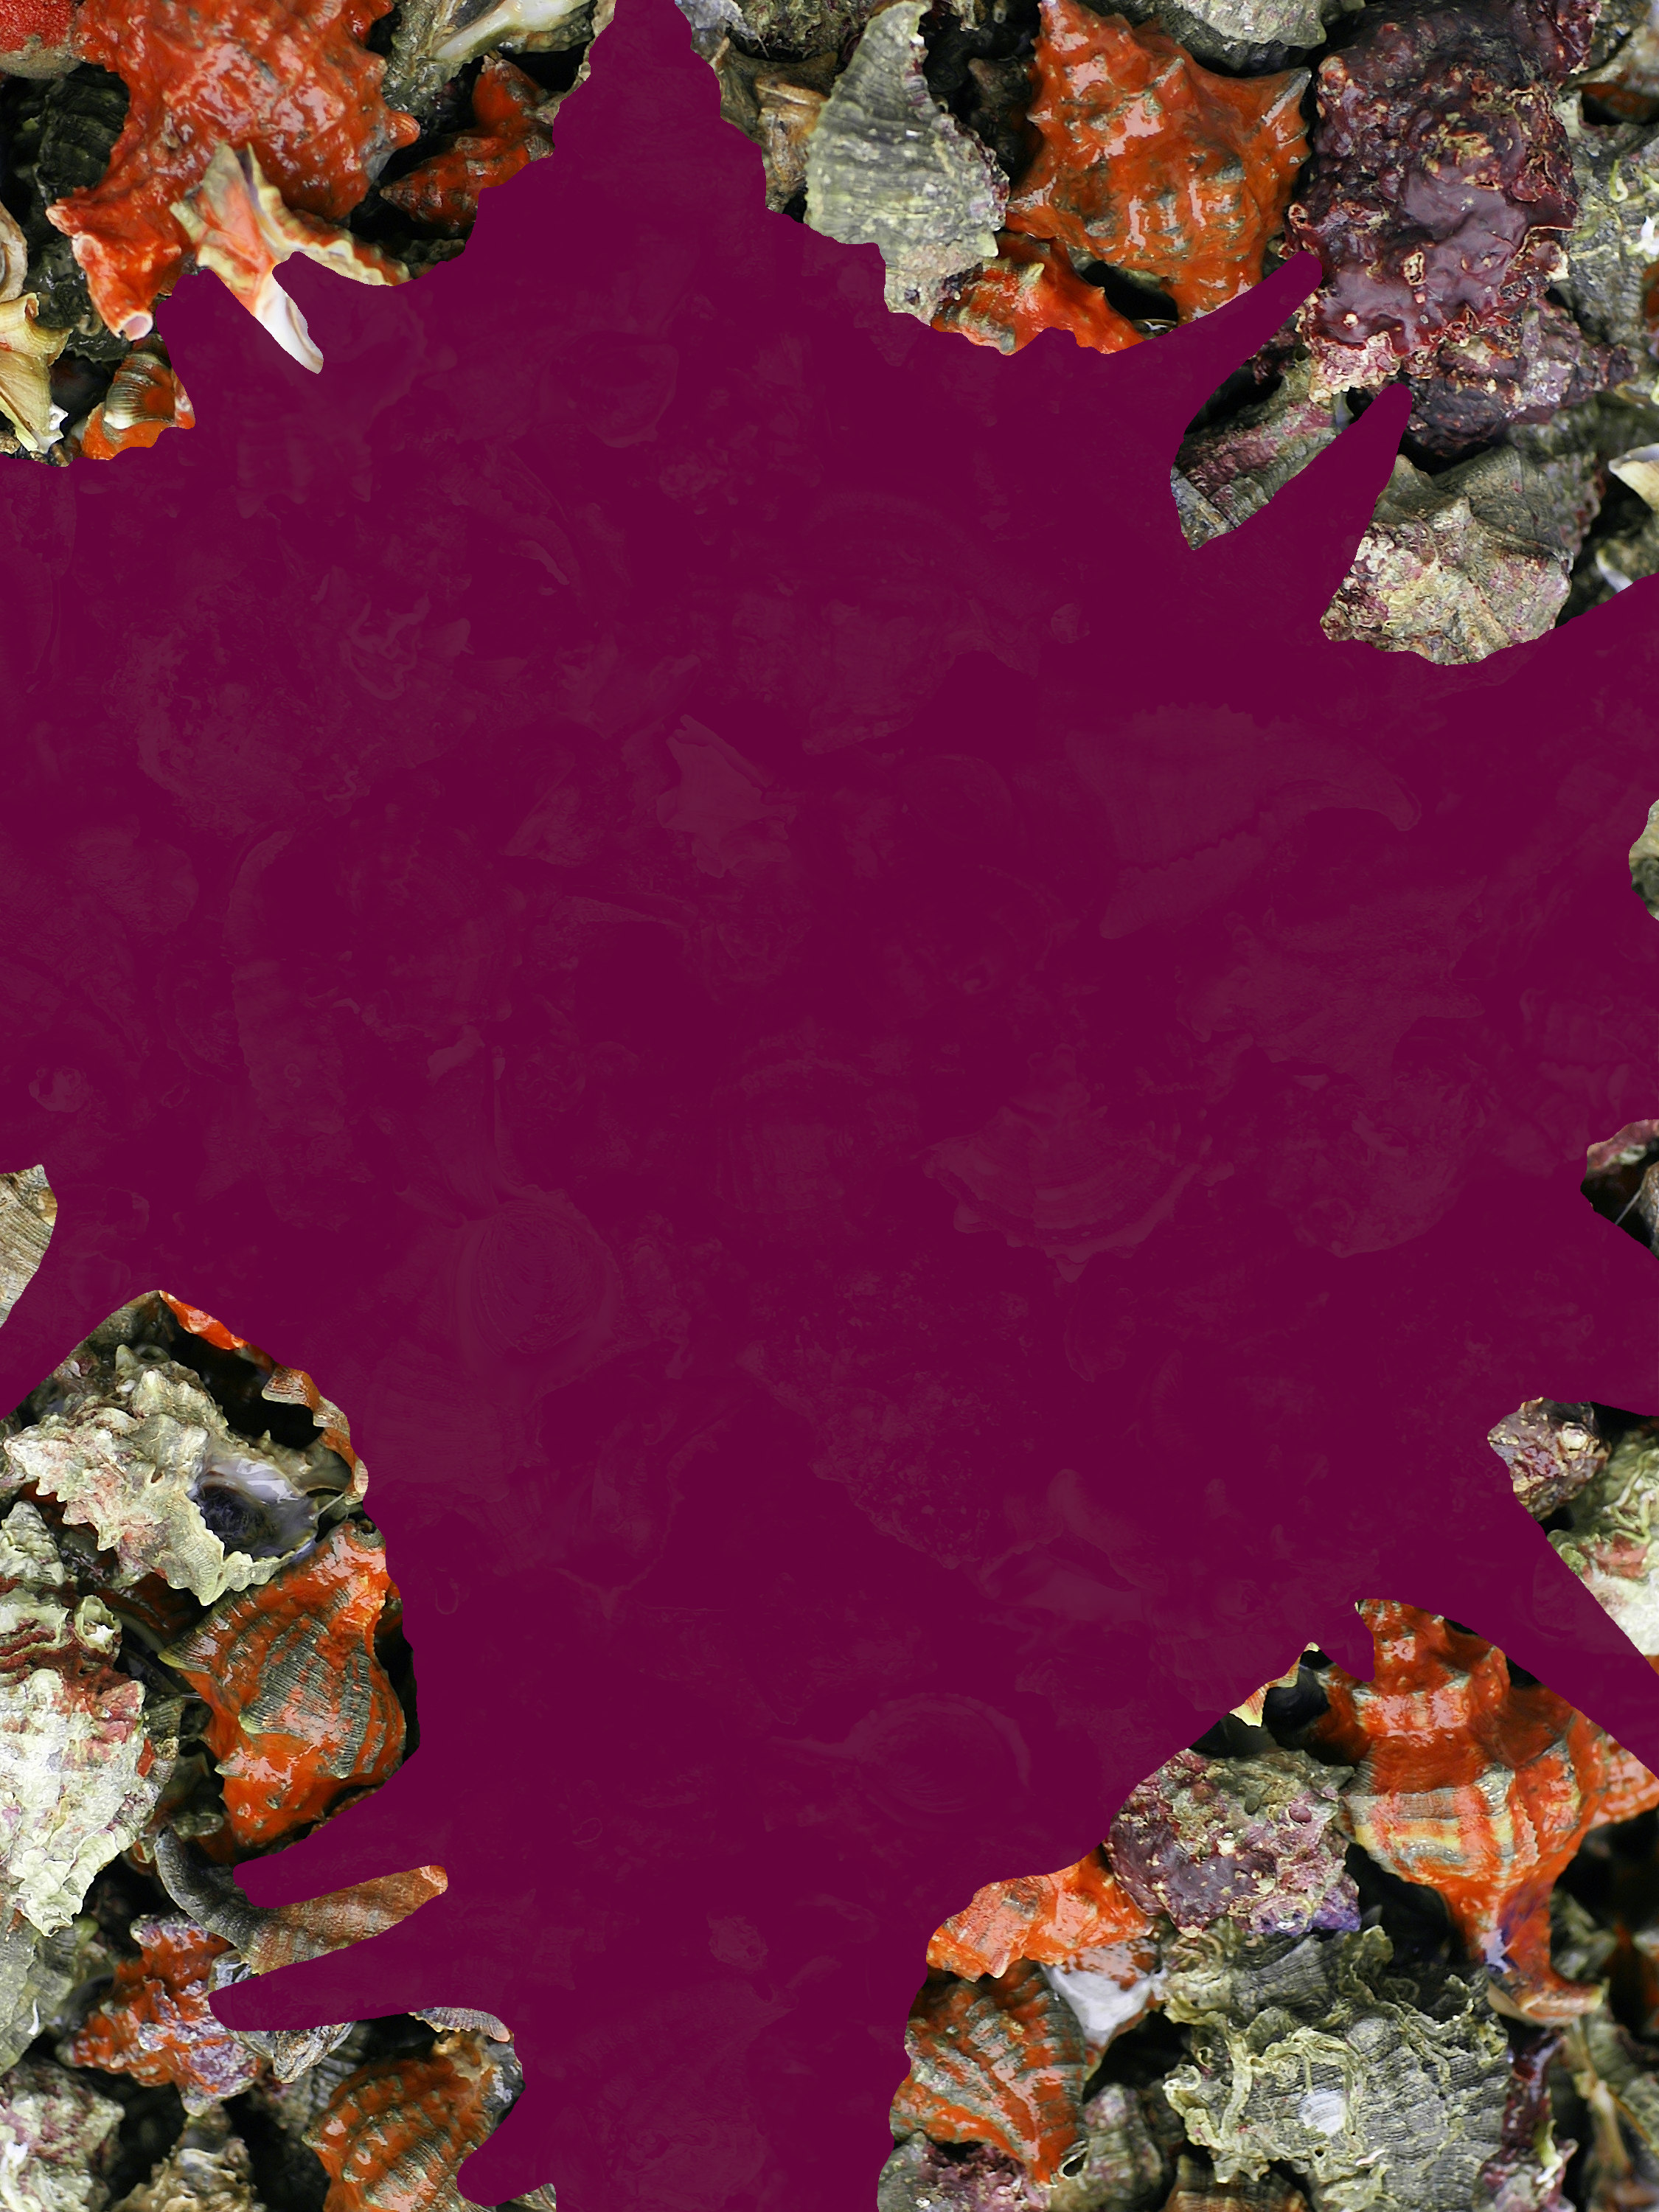
\includegraphics[width=\paperwidth,height=\paperheight]{murexpurple.jpeg}}
\begin{titlepage} % Suppresses headers and footers on the title page
	\centering % Centre everything on the title page
	%\scshape % Use small caps for all text on the title page

	%------------------------------------------------
	%	Title
	%------------------------------------------------
	
	\rule{\textwidth}{1.6pt}\vspace*{-\baselineskip}\vspace*{2pt} % Thick horizontal rule
	\rule{\textwidth}{0.4pt} % Thin horizontal rule
	
	\vspace{0.2\baselineskip} % Whitespace above the title
	
	{\scshape\Huge Opusculum de Purpurâ}
	
	\vspace{0.2\baselineskip} % Whitespace above the title

	\rule{\textwidth}{0.4pt}\vspace*{-\baselineskip}\vspace{3.2pt} % Thin horizontal rule
	\rule{\textwidth}{1.6pt} % Thick horizontal rule
	
	\vspace{0.2\baselineskip} % Whitespace after the title block
	
	%------------------------------------------------
	%	Subtitle
	%------------------------------------------------
	
	{\scshape \Large Fabii Columnæ,\\\large Lyncei, \emph{Nobilis Neapolitani}, \emph{Genere Romani}; }
 
        \vspace{0.1\baselineskip}

        {\scshape \small Romæ primùm, An. 1616. editum,\\et nunc iterùm Luci datum \\\emph{Operâ ac studio} }

        \vspace{0.1\baselineskip}
        
        {\scshape \Large Johann-Danielis Majoris,\\\normalsize Medicinæ D. } % Subtitle or further description
	
	\vspace*{0.2\baselineskip} % Whitespace under the subtitle
	
        {\scshape \normalsize \emph{Cujus novissimè accesserunt} annotationes quædam} % Subtitle or further description

	%------------------------------------------------
	%	Editor(s)
	%------------------------------------------------
        \vspace*{\fill}

	\vspace{0.2\baselineskip}

	{\small\scshape Kiliæ, 1675}
	
	{\small\scshape{Imprimebat Joachim. Reumannus, Academ. Typogr.}}
	
	\vspace{0.1\baselineskip} % Whitespace after the title block

        \scshape Internet Archive Online Edition% Publication year
    
	{\scshape\small Namensnennung Nicht-kommerziell Weitergabe unter gleichen Bedingungen 4.0 International} % Publisher
\end{titlepage}
\setlength{\parskip}{1mm plus1mm minus1mm}
\clearpage
\tableofcontents
\clearpage
\begin{center}
\emph{Reverendissimo ac Serenissimo Principi ac Domino},

Dn. Augusto Friderico,

{\footnotesize Heredi Norwagiæ, Electo Episcopo Lubecensi, Sleswigæ, Holsatiæ, Stormariæ, et Ditmarsiæ Duci, Comiti in Oldenburg et Delmenhorst, etc.}

Principi ac Domino Meo Clementisimo.
\end{center}
\paragraph{}
\emph{Salve, atque iterum humillimè mihi Salve, Serenissime Princeps, quem Regali ortum Sanguine, reducemque, ex Aulâ Regiâ, agitata propitio Mari Balthico ac Ventis Prora, incolumem iterum in has partes Cimbriæ advexit. DEO Ter-O. M. ante omnia ob id debentur Laudes: Hinc osculo devotionis adrepo Augustæ Dextræ Tuæ, Eique, in aliqua gaudii mei ostentationem, venerabundus subjicio editum meâ curâ perelagans Illustris Fabii Columnæ, Nobilis Neapolitani, Gente autem Romani, de Purpurâ Opusculum, quod Romæ antea (An. 1616.) impressum, propriâque Autoris manu, Tabulis æri incisis ornatum, sed difficilè hodie ampliùs reperiundum in Bibliopoliis, ut ab interitu vindicarem, tum et, ut esset præliminaris quasi portiuncula ededi à Me Theatri Naturæ Leopoldini, vel Physicæ Augustæ, Experimentali huic Seculo accommodandæ; transcripsi meâ Manu, ex Bibliothecâ Magni quondam Germaniæ Æsculapii, Sennerti, meoque impensu Figuris in Buxo factis, similiter exornavi; ac Nervum mihi incalescere ausus sum, ut Scriptum id de Regali materiâ, sicut jam antè Ecclesiastico Principi, Jacobo Sannesio, Romanæ Sedis Cardinali, ita nunc Episcopali Tuo Splendori, et Illustrissimis Meritis, dedicarem; cum aliquantò tutius ducam, quoties Clementiæ Tuæ recordor, ab aliquot annis mihi præstitæ, inter publicas Holsatiæ, Wagriæque de Reditu Tuo lætitias, ex alienâ fruge liberalem, quam planè mutum esse. Ad hæc peculiariter me ad Subjectissimum Cultum et Amorem obstrinxit jam pridem Tua Serenitas, dum minùs est dedignata superiori tempore, in Utinensi suâ Aulâ, plusculas horas constanter impendere, non minùs curiosè videndis, quàm clementissimè approbandis Experimentis variis, Anatomico-Opticis ad Explicationem Oculi, inque eo Visionis Inversæ, ad cognitionem item aliarum Partium, et ad Chirurgiam Infusoriam spectantibus, cum Technopægniis quibusdam aliis, humillimâ meâ curâ factis; et oblectationem Animi sui Excelsi ex his etiam minutiis venari.}

\emph{Quàm gratus itaque ac excellens aliàs est Rubor Rosæ præ Floribus aliis; vel Sanguinis Color in Corpore Animali; vel Auroræ in Cœlo, vel Minii in Terrâ, vel Purpuræ denique in Mari; tam grata mihi magis magisque renovabitur Indulgentiæ Tuæ Memoria, si, Serenissime Princeps, Columniana etiam hæc Purpura, in periculo obliviosæ noctis jam aliquo versarivisa, inter Augustos Clementissimæ Tuæ Dextræ amplexus reviviscere quasi, et novâ iterum Luce, pristinoque splendore frui possit. Subjungo Votum, ut DEUS diu feliciterque Serenitatem Tuam servet. Scrib. Kiliæ, d. 3.} 8 \emph{bris. 1674.}
\begin{center}

Reverendiss. T. Serenitati

{\footnotesize ac Valetudini, omni curâ}

{\footnotesize Devotissimus}

{\footnotesize Joh. Daniel Major, Phil. et Med. D.}

{\footnotesize Med. Pract. Prof. Publ. ibidem.}
\end{center}
\clearpage
\begin{center}
\emph{Illustrissimo et Reverendiss. Domino}

Jacobo Sannesio,

{\footnotesize S. R. E. Cardinali,}

{\footnotesize Suâ, omniumque Observatione Dignisimo,}

{\footnotesize Fabius Columna}

{\footnotesize perpetuam Felicitatem precatur.}
\end{center}
\paragraph{}
\emph{Quanti olim et usûs, et precii Purpura fuerit, AMPLISSIME CARDINALIS, vel solus} Plinius \emph{Historiæ suæ Naturalis libro Nono nos docere poterit; cujus hæc concepta sunt Verba:} Nepos Cornelius, qui Divi Augusti Principatu obiit, Me, inquit, Juvene Violacea Purpura vigebat, cujus Libra Denariis centum venibat, nec multò post Rubra Tarentina.

\emph{Rectè sanè. Nam et hodie non solùm magni Romæ æstimatur: sed et in VESTRO AMPLISSIMO SE. NATU PURPURATORUM, utraque Purpura, tàm Violacea, quàm Rubra, sibi locum invenit, Indumentis Vestris serviens. Et Rubra quidem, quam Tyriam olim Tarentinamque appellabant, in quotidiano amictu jucunditatis uti, sic Majestatis profectò plurimum præsefert: in Violaceà verò, quam Conchylium Veteres dicebant, Mœroris et Gravitatis itidem signa elucescunt. Et quid mirum, cùm antiquitùs Romanorum quoque Procerum Imperatorumque Vestes Purpureus Color decoraret: unde et Leges exstant, ne Murileguli (sic Infectores illi denominabantur) purpureo illo Colore, Sacri Muricis nomine indigitato, alias Vestes aut tingerent, aut Imperiales adulterarent.}

\emph{Atque sic quidem Antiqui Conchyliis Purpuris, sive Buccinis, Colorem hunc præstantissimum effingebant: quibus postera Ætas relictis, vel propter Inscitiam, vel majorem impensam, ignoro equidem, Cocco et marino Bryo Vestes tingit purpureas; sicut transalpinam Galliam fecisse}, Plinius \emph{refert:} Herbis, \emph{inquit}, Tyrium atque Conchylium tingit, omnesque alios Colores; nec quærit in profundo Murices.

\emph{Verùm cum Ego studiosè admodùm rimarer, quodnam esset Conchylium hocce, ad Purpuræ Tincturam aptum, illud tandem perquirendo inveni: inventum autem ut Lucem adspiceret, Commentariolo quodam meo enixè elaboravi. TU enim, CARDINALIS AMPLISSIME, unicus occurristi, tùm quia Sacrâ Purpurâ vestiris, tùm quia in fulgentissimo illo Purpuratorum Consessu magni momenti negocia summâ cum Laude, omniumque Admiratione sæpenumero tractas; tum etiam quando à gravioribus semotus aliquantulum Curis animum refocillare intendis, Naturalibus Studiis adeò delectaris, ut instructissimum, nunc Hortum tâm Exoticis, quàm Nostratibus plantis habeas; ex quo cum Purpureum illum elegantissimum, atque rarissimum Hyacinthum nactus fuerim, quem Tuâ Humanitate fretus, quod Tu Solus illo Romæ potireris, SANNESIUM nuncupavi; non abs re erit, si et hic cum Cochleâ meâ Purpureâ ad Te confugiat, quam vel sola Umbra Purpuræ Tuæ Cardinalitiæ fovere et illustrare poteris.}

\emph{Quod ubi à TUA benignitate impetravero, neque Zoilorum mordacem dentem, neque Invidorum sinistram Mentem pertimescam. Quodsi verò etiam gratum hoc meum studium intellexero, gratiorem ac festiviorem alteram, ac Rubram illam Purpuram, quam indagare non desino, quamprimùm sub eodem Tuo Amplissimo Nomine in studiosorum gratiam proferre elaborabo. Interim TE DEUS OPT. MAX. diutissimè incolumem præstet, altioribus TE Honoribus reservans. Vale.}

\clearpage
\section*{Idem Autor Ad Lectorem Ostracoptam}
\paragraph{}
\emph{Testaceorum Tractatio multiplici varietate perjucunda, et vel ipsa Purpura nobilis paucos quidem cùm ex Antiquioribus, tùm ex Recentioribus Physicos detinuit. Ex omnibus tamen, qui de illis verba fecerint, Neminem ipsa Testis inhabitantia Animalia considerasse, variasque eorum effigies tradidisse, mirum sanè videri potest. Ut enim animadvertere incipimus, minimè parvi facienda est Animalis ipsius Imago et natura, ex cujus differentiâ etiam Testæ differentiam provenire est necesse. Observavimus diversum in Cochleâ, ac in Purpurâ Animal, variaque variis in Testis, nec etiam similia esse, quæ in Cochleæ modò formatis Testis, licet solâ magnitudine, vel Colore tantùm inter se eædem Testæ differant, ut in Ianthinâ Cochleâ, et aliis. Commune quidem habent Turbinata omnia, quod Limbo sint prædita quodammodo simili, quo gradiuntur, sive repunt; cervice verò et aliis non solùm à Terrestribus Cochleis differunt, sed inter se etiam Colore variare, manifestum est.}

\emph{Exponere igitur hîc voluimus Purpuram, rarioribus nonnullis Testaceis adjunctis, Testas simul, ipsaque Animalia, in Physicam Contemplationem adducentes, unde illorum differentia innotescere possit. In his interim eam inspice, et perpulcrâ fruere varietate: postmodum enim, DEO dante, in aliorum Testaceorum Observationibus, quæ exhibituri sumus, plenius quid videre licebit. Vale.}
\clearpage
\section{Caput 1. --- \emph{De Purpurâ Testaceo, Purpuram fundente, et Ejus Animali}}
\paragraph{}
§. 1. Purpuræ vox sive Nomen, ab Antiquioribus non tàm generis loco prolata, quàm Speciei ; quin Animal etiam Testaceum genere distinctum, ex quo purpureus ille Color eximebatur, eundemque; Colorem extractum, pallore variantem, complectens; Muricis etiam Conchyliique denominatio, Rerum atque Vocum confusionem apud Recentiores peperisse videtur. Verùm id Latinorum causâ potiùs, quàm Græcorum Lectione contigisse, patebit.

§. 2. Ut autem differentia Vocum atque Rerum innotescat, Confusio etiam distinguatur, Veterum Auctorum aliquot Loca priùs examinanda, et præponenda esse, operæ precium visum fuit.

§. 3. Purpura igitur Color, et Purpura Testaceum Animal, quod sub nomine Conchylii et Muricis ab antiquis acceptæ sint, apparebit: eaque nomina quando propriè vel impropriè, aut in genere vel specie illi comprehenderint, priùs distinguere conabimur.

§. 4. Conchylium, tanquam summum genus Concharum et Testaceorum, à \emph{Plinio}\footnote{\emph{lib. 9. cap. 36.}} usurpatum censemus, de Purpurâ loquente, cum ait: \emph{Lingua Purpuræ digitali longitudine, quâ pascitur perforando reliqua Conchylia}. Et de Lunæ potestate verba faciens\footnote{\emph{lib. 2. cap. 99.}} ait, \emph{ideò cum incremento ejus augeri Conchylia}. Quod \emph{Horatius}\footnote{\emph{lib. 2. Sat. 4.}} Metro expressit, cum ait:
\begin{quotation}
\hspace*{12mm}\emph{Lubrica nascentes implent Conchylia Lunæ.}

Et alibi: --- --- --- \emph{simul assis}

\hspace*{12mm}\emph{Miscueris elixa, simul Conchylia Turdis.}
\end{quotation}
\paragraph{}
\emph{Plinius}\footnote{\emph{lib. 9. cap. 29.}} de Polypi naturâ: \emph{Vescuntur Conchyliorum carnes, quorum Conchas complexu crinium frangunt}. Idem\footnote{\emph{lib. 9. cap. 10.}} de Testudinibus loquens: \emph{In Mari Conchyliis vivunt, tantâ oris duritie, ut Lapides comminuant}. Et alibi\footnote{\emph{lib. 9. cap. 17.}} de Mullis inquit: \emph{Laudatissimi Conchylium sapiunt}. Et alibi,\footnote{\emph{lib. 6. cap. 21.}} de Indiæ Insulis: \emph{Bibaga Ostreis} et \emph{Conchyliis referta}. Quanquam et hæc inferiora loca pro Turbinatis tantùm accipienda si quis esse dixerit, medium genus constituere viderentur.

§. 5. Nos verò pro inferiori Genere Turbinatorum, sive Concharum, Purpuram fundentium, ab eodem \emph{Plinio}\footnote{\emph{lib. 8. cap. 48.}} Conchylium acceptum putamus, cum inquit, de Lanarum generibus et Tincturâ disserens: \emph{De reliquarum infectu suis locis dicemus, in Conchyliis Marinis, et Herbarum naturâ}. Apud \emph{Lucretium}\footnote{\emph{lib. 6.}} de Rerum Naturâ:
\begin{quotation}
\emph{Purpureusque color Conchyli jungitur unâ,}

\emph{Corpore cum Lanâ.} --- --- ---
\end{quotation}
\paragraph{}
Et \emph{Catulius} de Nuptiis Pelei et Tetidos:
\begin{quotation}
\emph{Tincta tegit roseo Conchylis Purpura fuco.}
\end{quotation}
\paragraph{}
§. 6. Sic etiam \emph{Vitruvius}\footnote{\emph{lib. 7. cap. 13.}} antiquior \emph{Plinio}, Conchas, ex quibus Ostrum præstantissimum omnium purpureorum Colorum arte conficiebatur, appellavit, cum inquit: \emph{Id autem excipitur ex Conchylio marino, quo Purpura inficitur}, etc. Additque modum præparationis. Et in fine Nominis rationem afferens, inquit: \emph{Et quod ex Concharum marinarum Testis eximitur, ideò Ostrum est vocitatum}. Apud Poêtas etiam Ostrum Color est Purpureus; ut apud \emph{Juvenalem}\footnote{\emph{Satyr. 2.}}:
\begin{quotation}
\emph{Et Princeps Tyrio vestem prætexuit Ostro.}
\end{quotation}
\paragraph{}
Eundem Colorem \emph{Virgilius}\footnote{\emph{lib. 2. Georg. v. 506.}} Sarranum dixit:
\begin{quotation}
\emph{Et gemmâ bibat, et Sarrano dormiat Ostro.}
\end{quotation}
\paragraph{}
§. 7. Sed \emph{Vitruvius}, tanquam Latinus, omisit verum Ostri Etymon, quod non est Latinâ derivatione factum, sed Græcâ. Testas quidem sive Conchas marinas Generis appellatione Græci dicunt Ὄστρεα et ὄστρεια, ex quibus Ostrum Latini purpureum colorem, et Ostracium ex Ostreâ dicunt. Græcis verò ex ὄστεον, quod est Ος, quia Ossium sit duritie Marina Concha, Etymon sumpsisse putat \emph{Eustathius}, sicuti Latinos à Testarum duritie, Testas. \emph{Athenæus}\footnote{\emph{lib. 3. cap. 12.}} tanquam generalissimum acceptum refert, cum ait: \emph{Solenistræ dicebantur, qui hujusmodi Ostrea colligebant}, ut inferiùs narrat; scilicet à Solenistrum capturâ.

§. 8. Conchylium prætereà Infecturæ genus propriè dici, et à \emph{Plinio} sic etiam usurpatum, satis est manifestum, ut nos existimamus: de Infecturâ siquidem Coloris Amethystini et Cocci loquens\footnote{\emph{lib. 9. cap. 41.}} ait: \emph{Et cum confecére Conchylia, transire meliùs in Tyrium putant}. Amethystinus quidem Color fiebat, eodem Autore, permixtis Pelagio et Buccino simul; aitque\footnote{\emph{lib. 9. cap. 38.}}: \emph{Summa medicaminum in Libras Vellerum Buccini 200. Pelagii 111. ita fit Amethystinus Color eximius ille}. Et alibi\footnote{\emph{lib. 9. cap. 36.}} ait: \emph{Concharum ad Purpuras et Conchylia eadem quidem est Materia, sed distat Temperamento. Duo sunt genera: etc.} Temperamenti differentiam \emph{Idem} docuisse videtur inferiùs,\footnote{\emph{lib. 9. cap. 39.}} cum ait: \emph{In Conchyliatâ Veste cætera eadem sine Buccino, præterque jus temperatur Aqua pro indiviso humani potûs excremento, dimidia, et medicamina adduntur: sic giganitur laudatus ille pallor, saturitate fraudatâ, tantòque dilucidior, quantò magis vellera esuriunt}.

§. 9. Conchylium etiam pro Colore intellexisse putamus suprà, de Purpuræ differentiâ; Testaceo scilicet Animali, ad Tincturam apto, ibi\footnote{\emph{lib. 9. cap. 36.}}: \emph{Calculosæ appellantur à Calculo maris, mirè apto Conchyliis}. Et superiùs: \emph{Sed unde Conchylii precia, quis, virus grave in fuco, color austerus in glauco, et irascenti similis Mari?} Et anteà\footnote{\emph{lib. 9. cap. 34.}} dixerat: \emph{Sed quota est porsio hæc, reputantibus Purpuras, Conchylia, Margaritas? Parum scilicet fuerat, in gulas condi Maria, nisi Manibus, Auribus, Capite, totoque Corpore à Fœminis juxta Virisque gestarentur? Quid Mari cum Vestibus? Quid Undis Fluctibusque cum Vellere?} etc. Et de Carthagine loquens alibi\footnote{\emph{lib. 5. cap. 19.}}: \emph{Nunc omnis ejus Nobilitas Conchylio atque Purpurâ constat}. Et alibi,\footnote{\emph{lib. 22. cap. 2.}} de Coloribus ex Herbis loquens: \emph{Transalpina Gallia herbis Tyrium atque Conchylium tingit, omnesque alios colores, nec quærit in profundo Murices}.

§. 10. Quod autem non sit aliqua Conchæ, sive Turbispecies, ad Purpuram inficiendam apta, quæ proprio nomine Conchylium specialiter, diversumque à Purpurâ et Buccino dicatur; jam satis ex supra-citatis Locis constare censemus. Veluti et hoc manifestum est, quod Conchylium nomen sit genericum Testatorum, scilicet Purpurarum, aut proprium Coloris illius purpurei dilutioris, Conchilium appellati, ut ex Capite trigesimo septimo, ac etiam præcedenti patet, in quo \emph{Plinius} clarè docuit, duo tantùm esse Genera Testaceorum, ad Purpuras et Conchylia Colores utilia, Buccinum scilicet et Purpuram, illorum notas afferens; atque eandem esse materiam. At Purpureum à Conchylii Colore, Temperamento tantùm differre: et quod ex Purpurâ solùm, absque Buccino, conficiatur: nec non Pelagiam Purpuram ad hunc colorem optimum conficiendum præferri, quæ calculosa dicebatur: nam Teniense levius atque dilutius erat. Prætereà pro quovis genere Colorum nulla alia materia recensetur à \emph{Plinio}, nisi Purpuræ et Buccini Concharum ex Marinis; nec unquam Conchylii Animalis, sive Testacei, suâ specie distincti notas vel historiam, apud aliquem Antiquorum hucusque descriptam reperimus.

§. 11. Conchylii verò proprius Color, qui cœruleus erat, dilutior, vel plenior, ab eodem \emph{Plinio} describitur simul cum aliis purpureis, colore saturatiore variantibus, cum de Vestium æmulatione cum Floribus historiam recitat, ibi\footnote{\emph{lib. 21. cap. 8.}}: \emph{In quibus unguento vicisse Naturam gaudens luxuria, Vestibus quoque provocavit eos flores, qui Colore commendantur, hos animadverto, Tres esse Principales: Unum in Cocco, qui in Rosis micat. Gratius nihil traditur adspectu, et in Purpuras Tyrias, Dibafasque, ac Laconicas: Alium in Amethysto, qui in Violâ: et ipse in Purpureum, quem Ianthinum appellavimus; Genera enim tractamus, in species multas sese spargentia: Tertius est, qui propriè Conchylii intelligitur multis modis: Unus in Heliotropio, et in aliquo ex his saturatior; alius in Malvâ, ad Purpuram inclinans; alius in Violâ Serotinâ, Conchyliorum vegetissima}.

§. 12. Ex quâ Descriptione Purpureum Colorem esse dicimus, qui magis ad rubedinem tendit, saturo satis Colore, ut Rosæ purpureæ; quem alibi\footnote{\emph{lib. 9. cap. 36.}} nigricantis Rosæ colore sublucentem dixit: alium dilutiorem, ut Violæ marinæ præcocis, quæ ἴον dicitur à Græcis. Altera verò Species Purpuræ illa videtur, quæ ex rubro magis ad cœruleum tendit dilutum, et dicitur propriè Conchylium, ut Heliotropii color vel purpureæ Malvæ; aut magis obscurum, ut Violæ, Serotinæ, quod est, Violæ purpureæ montanæ; de quo \emph{Virgilius}\footnote{\emph{lib. 4. Georg.}}:
\begin{quotation}
--- \emph{Violæ sublucet Purpura nigræ;}
\end{quotation}
\paragraph{}
qui alibi à \emph{Plinio} Austerus Color in Glauco, et irascenti similis Mari dicitur.

§. 13. Colorem hunc Conchylii sine Buccino fieri, tradit idem \emph{Plinius}, eâ ratione, quia Buccinum ad Rubedinem Rosæ, aut Cocco similem, ferè tendit: Purpura verò magis Violaceam emittit Saniem. Ideò leguntur verba illa in \emph{Plinio}: \emph{Rubens color nigricante deterior}: Deinde Pelagio alligari Buccinum, ut ruborem inducat, eâ ratione, quia nimiæ ejus nigritiæ dat Austeritatem illam, nitoremque, qui quæritur, Cocci, ut Sanguinis concreti speciem referat. Color iste Tyrius dicebatur; qui, ut melior effet; priùs Conchylia conficiebantur Pelagio satiatis Velleribus immatura, viridique Cortina non satis cocta, ne nimis evaderet nigricans Conchylium; deinde in Buccini Cortinam permutabatur, ut Ruborem superacciperet, atque ita permixtis viribus utriusque alter altero excitaretur Colore, aut adstringeretur, ut \emph{Idem} refert.

§. 14. Conchylium postremò dictum fuisse Colorem hunc, eâ ratione videri potest, ut sicut Ostrum ab Ostraceis derivatum esse existimatur, sic Conchylium à Conchis vel Conchulis marinis; quod Etymon \emph{Isidorus}\footnote{\emph{lib. 19. Orig. c. 28.}} habet. Et apud Græcos Κογχύλιον etiam pro omni Testaceorum genere, maximè vesco, apud \emph{Pollucem}\footnote{\emph{lib. 6. c. 15.}} dictum invenitur. Sed clariùs apud \emph{Athenæum}\footnote{\emph{lib. 3.}} ex \emph{Epicharmo}, ibi: ἀγε δέ παντόδαπα Κογχύλια, Λεπάδασ etc. \emph{affer omnigena Conchylia, Lepades, etc.} Et inferiùs ex \emph{Diocle}: Κράτιστα Φύσιν ῥῖναι των κογχυλίων πρὸς διαχώρησιν καὶ ὄρησιν, μυάς, ὄστρεα, κτένας, etc. \emph{Ex Conchyliis excellere ait alvo movendo, etc lotio ciendo, Mytulos, Ostrea, Pectines, etc.} Et inferiùs: \emph{Conchyliorum firmissimas Conchas, Purpuras et Buccinum}.

§. 15. Ex his denique rejicienda est eorum opinio, qui \emph{Dioscoridis} Testimonio uti volunt, ex Onychis historiâ decerpto; ubi, \emph{Crematum}, inquit, \emph{Conchylium idem efficit, quod Purpura et Buccinum}. Et sic esse ab illis animal sive Testaceum distinctum. Sed nos à Purpurâ et Buccino distinctum Conchylium hoc esse \emph{Dioscoridis} putamus, non quia specie differat, cum sit genus Concharum sive Turbinatorum; sed quia sit \emph{genus Palustre}, non marinum; sit que \emph{Aromaticum}, ut \emph{Idem}\footnote{\emph{lib. 6. de Dorycnio.}} refert, depascentibus illis Conchyliis Nardum herbam: quod Purpuram et Buccinum haut facere, quisquam refert.

§. 16. Nec minùs quàm alii hoc loco \emph{Dioscoridem} Conchylium pro genere Concharum sive Turbinatorum usurpasse censemus, ut ex Ipsius historiâ liquet, et alibi etiam, cum inquit: καὶ πάντα τὰ Κογχύλια ὠμὰ καὶ ὄπτα ἐθιόμενα, καὶ κάραβοι: \emph{Et omnia Conchylia, cruda, quàm tosta comesa} etc.

§. 17. Adde, Lacustres Conchas, sive Turbines, ad Tincturam aptas, nemo Antiquorum prodidit. Quare differre à marinis Infectoriis patet, sicut generis esse nomen. Non mirum igitur, si \emph{Onychem} eandem à \emph{Plinio} Ostracium dictam invenimus; Græco forsan more, ex Verbo \emph{Ostracea}, quod universa Testacea complectitur, ἀπὸ τοῦ ὀστρακοῦ deductum: sicut \emph{Ostrum} dici Purpureum colorem, à Testis Marinis latinè, ex \emph{Vitruvio} jam retulimus. Easdem Vires crematis Operculis palustris Conchylii \emph{Dioscorides} reliquis marinis Purpuris tribuit.

§. 18. Sic etiam malè intellectus \emph{Plinii} Sensus in Textu adducto ab iisdem dici potest, ibi\footnote{\emph{lib. 2. cap. 83.}}: \emph{Et per se Conchylio infecta Lana magnopere prodest}; Aurium scilicet malis; ut etiam apud \emph{Galenum}: κατὰ τρόπους τἦς πορφύρας, sive Κογχυλίου. Et apud \emph{Dioscoridem}, τὸν δὲ αὐτὸν τρόπον, καὶ κροκύδες καίοντας θαλασσίας πορφύρας, \emph{Eodem}, scilicet, \emph{modo uruntur Lanæ, marinâ Purpurâ infectæ}, sive \emph{Lanæ flocci}. Illud κροκίδες idem cum Lanâ Conchylio infectâ \emph{Plinii}.

§. 19. Nec etiam Conchylium à \emph{Plinio} Buccini loco acceptum putamus; ut alii; sed potiùs pro ipsâ Purpurâ, ex quâ tingitur; cum Purpura sine Buccino non rubescat, et ad cœruleum tendat, ut supra diximus de Pelagiis, Calculosis dictis ab eodem \emph{Plinio}\footnote{\emph{lib. 9. cap. 37.}} qui varias Purpurarum species recitat ibi, à loco nomine desumto. Quare de Conchylio jam satis dictum censemus.

§. 20. Sed non minor in Muricis nomine Observatio facienda est, ut quid sit propriè, quomodo sit à \emph{Plinio} aliisque acceptum, et quid differat à Purpurà, vel Buccino, innotescat. Murex nomen pro communi genere Testatorum omnium, à \emph{Plinio}\footnote{\emph{lib. 9. cap. 35.}} usurpatum, ex \emph{Mutiani} verbis liquet, de Remorâ loquens, ibi: \emph{Mutianus Muricem esse latiorem purpurâ, neque aspero, neque rotundo ore; neque in angulos prodeunte rostro, sed simplice conchâ, utroque latere se colligente}. Et alibi\footnote{\emph{lib. 9. cap. 33.}} pro Turbinatorum genere: \emph{Firmiores jam Testâ Murices, et Concharum genera}. Et pro Turbinatis ad Infecturam idoneis, ibi\footnote{\emph{lib. 2. cap. 2.}}: \emph{nec quærit in Profundo Murices}. Et alibi\footnote{\emph{lib. 32. cap. 7.}} dixit: \emph{Muricum vel Conchyliorum Testæ cinis}. etc. Quo loco Murex pro Purpurâ, vel Murex pro Turbinatis, et Conchylium pro universis Conchis acceptum videri potest. Et paulò inferiùs: \emph{Muricum genera sunt, quæ vocant Græci Colycia, vel Corythia}: nos Corycia legeremus, à verbo κορύκια. Quod autem Muricem \emph{Plinius}\footnote{\emph{lib. 9. cap. 37.}} pro Buccino dixerit, satis manifestè apparet, cum de Purpuris loquutus est: \emph{Latent, sicut Murices}. Qui locus ex \emph{Aristotele}\footnote{\emph{lib. 5. d. Nat. An. c. 51.}} transscriptus, habet pro Verbo \emph{Muricis}, Κήρυκες, ibi: τὰ μὲν γὰρ ὀστρακόδερμα τάντα φωλεῖ, ὁι ὀντὰ τέ ἐν τῇ θαλάττῃ πορφύραι, καὶ κήρυκες. Ut etiam inferiùs habetur: \emph{Mutuoque attritu Lentorem cujusdam Ceræ salivant, simili modo, ac Murices}. \emph{Aristoteles} habet, κηριάζουσι γὰρ καὶ ὁι κήρικες: et idem \emph{Plinius}\footnote{\emph{lib. 9. cap. 51.}} de Ortu Testaceorum habet: \emph{Quæ durioris Testæ sunt, ut Murices, Purpuræ, Salivario lentore}, etc. Et inferiùs: \emph{Purpuræ et Murices, ejus demque generis, Vere pariunt}.

§. 21. Apud Poëtas pro qualibet Acuminatâ Re acceptum reperimus Muricis nomen. \emph{Virgilius}:
\begin{quotation}
--- --- \emph{et acuto in Murice Remi}

\emph{Obnixi crepuére}. --- ---
\end{quotation}
\paragraph{}
Inde Muricatum nomen \emph{Plinius}\footnote{\emph{lib. 23. cap. 13.}} tribuit Sylvestrium Carduorum cacuminibus, cum dixit: \emph{Utrique Folia pauca spinosa, muricatis cacuminibus}. Quare impropriè Buccino Muricis nomen impositum videtur, cum propter aculeatos sive muricatos orbes, et extuberantes, quos habet Purpurarum genus, qui non sunt in Buccino, ut idem \emph{Plinius} ait, potiùs Purpuræ convenire sit dicendum; etiamque Muricis Epitheta omnia ab Auctoribus tributa, Purpuris convenire pateat, sicuti Purpura Tyria apud Poëtas; ut apud \emph{Ovidium}:
\begin{quotation}
\hspace*{15mm}\emph{Nec quæ de Tyrio Murice Lana rubet.}

Et \emph{Horatius}: \emph{Muricibus Tyriis iteratæ vellera Lanæ}.

Et alibi: \emph{Te bis Afro Murice tinctæ vestiunt Lanæ}.
\end{quotation}
\paragraph{}
§. 22. Tyrius color Purpureus à \emph{Plinio} Dibapha Purpura dictus est, quia bis tingebatur, et Pelagio primum Vellus mergebatur; quo nomine Purpura intelligitur, alio nomine Pelagia, ut diximus ex eodem \emph{Plinio}\footnote{\emph{lib. 9. cap. 37. 38.}} unde Tyrius Murex, est Purpura in Tyro tincta, ex Tyriis Muricibus, scilicet Purpuris. Sed et Murex Tyrius pro colore ipso acceptus fuisse, patet; ut etiam apud \emph{Virgilium}:
\begin{quotation}
--- --- \emph{Tyrioque ardebat Murice Lana.}
\end{quotation}
\paragraph{}
§. 23. \emph{Nomenclator Latinus} in Verbo Murex, Muricem à Græcis Conchylium dici putat, esseque Purpuræ speciem, Mensis expetitam. Ad id \emph{Martialem} citat, qui ait:
\begin{quotation}
\emph{Sanguine de nostro tinctas Ingrate lacernas}

\emph{Induis: et non est hoc satis; Esca sumus.}
\end{quotation}
\paragraph{}
Et \emph{Isidorus}\footnote{\emph{lib. 2. origin. cap. 6.}} refert: \emph{Murex Cochlea est Maris, dicta ab acumine et asperitate, quæ alio nomine Conchylium nominatur, propter quod circumcisa ferro, lacrymas coloris purpurei emittat, ex quibus Purpura tingitur, et inde Ostrum appellatum; quod appellatum, quod hæc Tinctura ex Testæ humore elicitur.}

§. 24. His igitur jam satis apertè ostensum fuisse arbitramur, Conchylium et Muricem esse Purpuræ Synonyma, quorum alterum à Conchis nomen, alterum ab Aculeis, qui alio nomine Murices dicuntur, sumsisse apparet: Purpuræ verò appellationem non solùm pro ipso Testaceo Animali accipi, sed etiam pro ipsa Tincturâ, et Colore; ut à \emph{Plinio},\footnote{\emph{lib. 9. cap. 35. initio.}} ibi: \emph{Sed quota hæc portio est, reputantibus Purpuras, Conchylia, et Margaritas?} Et alibi\footnote{\emph{ibid. in sine.}}: \emph{Conchylia et Purpuras omnis ora atterit}. Et\footnote{\emph{lib. 5. cap. 19.}} de Carthagine: \emph{Nunc omnis ejus Nobilitas Conchylio atque Purpurâ constat}. Et alibi,\footnote{\emph{lib. 35. cap. 6.}} de Purpureo colore pingendo verba faciens: \emph{Si Purpuram facere malunt, cœruleum sublinunt, mox Purpurissum ex Ovo inducunt}. Purpurissum verò, \emph{eodem autore}, fit ex Cretâ Argentariâ et Purpuræ Sanie, quod idem cum Ostro \emph{Vitruvii} esse videtur. Et alibi\footnote{\emph{lib. 9. cap. 36.}} manifestiùs: \emph{Concharum ad Purpuras et Conchylia eadem est materia, sed distat Temperamento}; ut suprà retulimus.

§. 25. Quid autem distet Purpura à Conchylio, nunc videndum. Nam etiam objicitur, \emph{Plinium} distinxisse Purpuram à Conchylio, cum inquit: \emph{Sed quota hæc portio est, reputantibus Purpuras, Conchylia, et Margaritas?} Et alibi: \emph{Conchylia et Purpuras omnis ora atterit}: et similia aliis locis. Quibus responsum jam esset ex supra memoratis observationibus; sed distinctiùs, ut omnia sint clara, addimus: Purpuram his locis à Conchylio esse distinctam, non Materiâ, quæ eadem est, (ut idem \emph{Plinius} retulit, cum dixit: \emph{Concharum ad Purpuras et Conchylia eadem est materia},) sed Colore. Nam, ut diximus, Purpura rubescit; Conchylium simile Violæ Purpureæ. Adde; Purpureo colori admixtum est Buccinum, quo carere asseritur Conchylium. Sed aliis locis à Conchylio distinguitur, tanquam Species à Genere; ut, cum idem \emph{Plinius} dixit: \emph{Lingua Purpuræ Logitudine digitali, quâ pascitur perforando reliqua Conchylia}: Et similibus, ibi, \emph{Conchylia} genus est non modò Turbinatorum, sed etiam Concharum omnium.

§. 26. Hâc denique Distinctione facilior remanet Purpuræ Animalis investigatio, à nemine traditi; sed nec forsan à quopiam Recentiorum visi, quamvis illius Historia satis ab \emph{Aristotele}\footnote{\emph{lib. 4. de N. Animal. c. 4. et lib. 5. c. 15.}} et \emph{Plinio}\footnote{\emph{lib. 9. cap. 36. et inde.}} descripta inveniatur: quam hîc inserere et repetere, multum molestumque esset. Illas tantùm notas recitabimus, quas in testaceo à Nobis proposito, observare licuit.

\begin{figure}[H]
\centering
\includegraphics[width=0.7\textwidth,keepaspectratio]{figs/001-goldenrod.png}
\caption{\emph{Murex trunculus.}}
\end{figure}
\paragraph{}
§. 27. Testa hæc parva est, Regiæ Nucis, adhuc carnoso regmine obducta, magnitudine, (quanquam ejusdem generis inanes Testas quadruplo majores habeamus, atque maximas asperiores) à vulgari Purpurâ \emph{Rondelitii}, quæ Neapoli Sconciglio appellatur, in his differens; Cortice quippe rugosiore, colore fusco, aut cinericeo, veluti Limo obducto, quandoque flavicante, et Fasciis distincta oblique purpurascentibus, Turbinis effigie oblongiore, ac etiam angustiore, eò quod non sit ita ventricosa: Aculeis illis, sive Muricibus longis, caret; verùm illorum vice brevibus et crassioribus horret Tuberculis, quo etiam modo et reliquæ Testæ supradictæ \emph{Rondelitii} Purpuræ non rarò inveniuntur. Non enim omnes illius generis Testæ longioribus Clavis horridæ observantur; sed brevibus admodùm Tuberculis, ut in Nostrâ propositâ.

§. 28. Differt etiam, quia bevi admodùm tubulo, vel Canali, oris pars superior definiatur, ut in Buccino, sed circa columellæ partem aspero, et auriculato vel umbilicato, à tribus vel quatuor prominentiis, quæ anteà Tubuli sive Canales, ex quâ Lingua ad usum proferebatur, fuére. Ab his dependent tuberosæ, atque parùm muricatæ Striæ, Testam per longum exasperantes, ut in extremâ oris margine, quâ Testæ os definitur, observatur: quibus signis illius Annos numerari posse censemus; quamvis Orbes \emph{Aristoteles}, et illum sequutus \emph{Plinius},\footnote{\emph{lib. 9. cap. 36.}} velint esse, cum dixit: \emph{Patet per Orbes, quibus totidem, quot annos habent}, etc. Non enim ex \emph{Orbibus}, quibus claviculatim contorquentur Testæ omnes, Anni earum observari debent; cùm Nos totidem Orbes, et quandoque plures, habere parvas et exiguas ejusdem generis Testas, quos maximas habere, observavimus in plerisque Turbinatorum generibus, si Orbis nomine quamlibet orbiculatam ventricosam partem, claviculatim intortam Testarum, esse dicas, ut Græcè legitur, καὶ καθ ᾽ ἕκαστον ἐνιαυτὸν φαρενά ἐστι ἡ ἄυξησις τοῖς διαστήμασι, τοῖς ἐν τῷ ὀστράκῳ τῆς ἕλικος. Et Latinè: \emph{Et in singulos Annos manifestum est Incrementum Distinctionibus illis, in Testaceo Volutarum}.

§. 29. Nos autem, quot habent Distinctiones in Volutis, quæ ab antiquioribus Oris, sive Canalis ad Linguæ usum Extuberantiis ortum ducunt per longum Volutarum, tot Annos habere, certiorem notam esse putamus. In \emph{Rondeletii} Purpurâ clavatâ quamlibet muricatam [Oram] anni illius Incrementum apertiùs ostendere dicimus. In Buccino verò Striato, ac etiam in Turbine Magno \emph{Ejusdem}, quem nos \emph{Plinii} Buccinum censemus, et in vulgari Buccino, manifestius apparet augmentum Testæ, ob lævitatem, et laxiorem, minùsque frequentem limbosam extuberantiam, quæ dimidium ferè singularum Volutarum orbem intercipere observatur.

§. 30. Hujus limbosæ majoris Extuberantiæ causam esse puramus, quia cum statuto tempore quotannis lateant Conchæ, Scopulis Oris margine adhærente, vis illa, Testæ incrementum addens, compressu adhærentiæ Saxo, non potest marginem oris Testæ produceve in orbem; quare crassescere circa extremum oris oportet. Manifestum esse apparet, quia non paucas habuimus Testas villosas omnes, præter recentem illam additionem ex Anni præteriti distinctione, quæ lævis et nitida erat; novumque incrementum esse, nemo ambigit. Atque ex hâc observatione non tantùm Annos septem Purpuras vivere, sed bis septem et plures, esse censendum: Buccinas verò, ob celeriorem auctionem, et laxiores distinctiones, pauciores.

§. 31. Nec obstat \emph{Aristotelis} et \emph{Plinii} auctoritas; cum Testæ omnes, ut diximus, parvæ atque maximæ, totidem habeant claviculatos Orbes, magnitudine illorum annosæ ab infantibus differentes, nec habitu aut proportione variantes. Imò in exiguis quandoque plures Orbium anfractus observavimus; quos deinde atteri ob tenuitatem, aliis supercrescentibus, censemus, ob Animalis volutationem, et Testæ imbecillitatem. At mediocris magnitudinis Testæ non minores Orbes habent maximis: quod si esset, longioris Turbinis essent majores parvis; quod contrà observatur, cùm omnes eundem Orbium numerum, et suam Symmetriam retineant.

§. 32. Causa esse potest, quia Testæ, quæ brevi et obtuso turbine sunt, et Effigie ventricosæ, oris marginem producendo, non gradatim in claviculæ speciem, per inferiorem orbem adscendunt; sed per eundem orbem pluries circumaguntur, descendendo potiùs quàm adscendendo, ut ventriosiores efficiantur, non longiores. Testæ verò, quæ magis oblongo sunt turbine, aliæ bis eundem orbem ambiunt, aliæ semel tantùm; ut sunt Turbines illi tenues digitali crassitie, qui detectos habent Orbes, atque in Persico Turbine, à Nobis aliàs exhibito, et aliis Turbinibus verioribus apparet. Qui Conchas Persicas Cochleam \emph{Rondeletii} maximam rugosam, Muricem Coraloidem \emph{Ejusdem}, et similes observavit, illarum Oris marginem imam, circa Orbem levem inveniet, atque Orbem magis operientem, ita ut Annis potiùs obtusiore Turbine annosior Testa, minùsque conspicuo inveniatur. Quare fallax est Orbium numerus ad Observationem Annorum.

§. 33. Sed ad Testam redeamus propositam. Intùs lævis est, Vitri modo splendens, colore obsoletè purpureo, vel cœruleo, aut flavicante, obliquè percurrentibus purpuro-nigris Maculis ex Oris margine in internâ ventriosâ parte. Operculum habet rugosum, tenue, fuscum, animalis capiti annexum et innatum, incrementum accipiens cum ipso Animali: nota est, rugosa superficies orbiculatim. Animal continet, effigie Cochleæ terrestris, carne flavicante, densis Maculis, ex cœruleo purpurantibus depicta, aliis exiguis luteis immixtis, præfertim in cervice. Corniculis verò à Terrestri Cochleâ variat: hujus quidem in acutum desinunt, et Oculi non in summo, ut in Terrestribus, sed supra medium Corniculorum observantur, ubi cornicula veluti resecta, per longum tenuiora efficiuntur. Oculis verò aliquando tueri Corniculis supra illos incurvatis, ut in Picturâ notatur, observavimus; ac etiam partem illam, supra Oculum, Corniculorum contrahere, ut nonnisi reliquum appareat, in Oculos desinens, crassius. At quando intueri putatur recta, tota exserta et firma Cornicula, extensaque habet.

§. 34. Differt etiam, quia Linguam ex Canali exserit, parum extra Canalem, Cochleis deficientem, colore purpureo, et ab illâ Aquam exspuere vidimus, fistulæ modo, contrahentem, branchiarum vicem explentem. Cum graditur, Limbo utitur extenso, ut Cochlea, Corpus deinde contrahens, iterumque Limbum producens, quem latum habet. Testam aliquando gaudet circumagere, illam in totum extollens, corpore in basis modum ad hoc elato. Colore tantùm obscuriore differt ab aliis vulgaribus aculeatis Purpuris \emph{Rondeletii}, dictis etiam \emph{Sconcigli Spinosi} vulgò; sicut et hæc etiam \emph{Sconciglio} appellatur, sed aliis distinctiùs vulgò \emph{Carosa} nomine dicitur, quasi spinis detonsa et carens, quam copiosè Neapoli propè Urbem in arenosis Piscatores venantur, Pulmonum frustulis, junceis Cratibus superimpositis allicientes, ut \emph{Aristoteles} olfacere censuerit.

§. 35. Hanc Littoralem potiùs, in Arenosis degentem, quamvis in profundo Mari, diceremus Purpuram, purpurocœruleum colorem fundentem: sed quare non omnes Purpuram fundant ejusdem generis, et eodem tempore captæ inter quamplurimas, quæ tot anno capiuntur, et semper aliquæ colorem habeant, hucusque ignorare fatemur.

§. 36. Venales habentur in foro quotidie; Cibis quidem expetuntur, elixæ ac tostæ, vel aliis modis. Capiuntur etiam propè Misenum Promontorium in Puteolano Mari, loco, nunc vulgò \emph{Mare Mortuum} appellato, ubi Maris æstus non recipitur, Portusque censetur olim ab Agrippâ et Augusto constructus. Hujus tantùm Testæ effigies ab aliis Recentioribus vario nomine imposito conspicitur depicta; à nemine verò hucusque interno Animali observato, nedum purpuream Saniem fundente. \emph{Plinius} Puteolanas Purpuras laudat: an de his intellexerit, aliorum sit judicium. Capiuntur etiam toto Maritimo tractu Australi, in Sinu Formiano olim dicto, nunc Molæ oppidi, ubi primùm in Mensâ tostas esitantes Purpuram fundere, et digitos, et linteos inficere observavimus.

§. 37. Harum usum, sicuti Buccinorum, non tantùm propter inscitiam ac magnam impensam ac molestiam neglectum putamus; sed ob maximam Fuci copiam, quem vulgus \emph{Roccella} denominant, quo nunc Infectores pulcherrimam Purpuram conficiunt, Sericia inficientes variis colorum gradibus, minore labore ac impensâ, et maximo lucro: tantùmque nobis hodie cùm Esca sint, non possunt \emph{Martialis} exprobrationem evitare, cum inquit:
\begin{quotation}
\emph{Sanguine de nostro tinctas, Ingrate, lacernas}

\emph{Induis; et non est hoc satis: Esca sumus.}
\end{quotation}
\paragraph{}
§. 38. Tarenti hucusque accepimus, Officinarum vestigia Purpurariorum conspici, atque etiam ex Testarum fragmentis acervos esse, quæ olim forsan, ut \emph{Plinius} refert, Augusti tempore fuere, Nepotis Cornelii testimonio, ibi\footnote{\emph{lib. 9. cap. 29.}}: \emph{Me}, inquit, \emph{juvene Violacea Purpura vigebat, cujus libra denariis centum veniebat, nec multò post rubra Tarentina}.

§. 39. Rubens Color nigricante deterior, à \emph{Plinio} dicitur; nisi Color sit nigricans adspectu Sanguinis concreti, qui non sine utriusque, Purpuræ et Buccini, mixturâ fieri poterat, quâ vel Amethysti, vel Tyrii, juxtà medicaminis quantitatem, Color fiebat, ut idem \emph{Plinius}\footnote{\emph{lib. 9. cap. 38. et inde.}} retulit.

\section{Caput 2. --- \emph{Cochleæ Iänthinæ cum Animali, exactior Icon et Historia}}
\paragraph{}
Depinximus atque descripsimus hanc, à Nobis aliàs obiter observatam Cochleam minùs rectè. Nunc autem Anno 1609. in oppido, dicto \emph{Torre della Nuntiata}, in Vesuvii Montis radice, ad Maris oram, inter Pompejanum et Stabii Ruinas, Majo Mense, flantibus Occidentalibus, maximoque Maris impetu illic æstuantibus undis, abjectas inter alia Cochleas multas, ex his adhuc viventes colligi curavimus: Maris Aquâ repleto quodam vase, Conchisque injectis, ut vivere possent, illarum Animal observavimus prodiens.

§. 2. Abomnibus Cochlearum Terrestrium et Maritimarum Animalibus reliquis, quas hucusque vidimus, hujus Animal valdè differt. Huic Penis arrecti facies est, glandem habens, in cujus extremo Fabam exprimit, rimam pro ore in medio, fœmininum ferè Sexum referens, rubescente magis internâ parte, cum reliquum Animal ex obsoletâ cœruleâ Purpurâ candicet: circà medium utrimque Appendices habet binas, quarum altera exterior major; earumque acies magis saturo colore purpurascunt.

\begin{figure}[H]
\centering
\includegraphics[width=0.7\textwidth,keepaspectratio]{figs/002-goldenrod.png}

\end{figure}
\paragraph{}
§. 3. Ima pars Animalis propè testam rugosa est, et denique limbosa, ut in congeneribus; non tàm oblonga, nec acuta, sed rotundior; sub quâ copiosam, extuberantem satis, atque veluti cartilagineam Spumam vitream fundebant omnes, non secùs, ac aquâ diluto sapone multo, et concussâ, atque paleæ vel alterius rei exiguâ fistulâ intinctâ, et inflatâ, paulatim evenit, ut puerorum mos est Neapoli; quæ Sphærulæ veluti vitreæ inflantur, et denique à fistulâ dimittuntur ex fenestris. Jocum non jucundum!

§. 4. Copiosum spontè evomunt Conchæ istæ succum Purpureum Violaceum, ut seipsas inficiant et colligentium manus: et paxillo, vel acu sauciatâ Animalis cervice, tres aut quatuor guttæ ex testâ decidunt, et quidquid tangunt, inficiunt, purpureo cœruleo colore admodùm hilari, ut nihil suprà commendari possit; charta vel album aliud Lineum infectum, quandoque variat maculis, colore ad rubrum inclinantibus: adeòque infectura hæret, ut vix lotione ex mi queat; undè et ipsa Testa infecta reperitur, quæ, ut diximus aliàs, tenuis est, circa imas Volutas candicans, tribus tantùm Volutis constructa, Limbo circà umbilicum elato admodum, quod nec in aliis Cochleis observatur, et ab illis differre hâc etiam notâ conspicitur.

\section{Caput 3. --- \emph{Turbo Exoticus Umbilicatus}}
\begin{figure}[H]
\centering
\includegraphics[width=0.55\textwidth,keepaspectratio]{figs/003-goldenrod.png}

\end{figure}
\paragraph{}
§. 1. Hunc Romæ apud quendam industrium hominem cum aliis non negligendis testis vidimus, atque raritate allecti, iconem delineavimus, notasque addidimus. Differt ab aliis Recentiorum, et à me descriptis, quod obtusus sit cacumine, circa medium tenuior; deindè æneæ nolæ effigie in latitudinem se diffundens, atque, quod præcipuum huic est, in medio Umbilicatus.

§. 2. Crassa est Testa, gravis, cortex superior rugosus, candicans, ad pallidum vergens; maculis obliquis roseo colore variegatus tam circa Umbilicum, quàm in reliquis Volutis; derasus, vel cortice extimo mundatus, argenteo Margaritarum nitore quodammodo splendet, non admodum, ut in parvis nostratibus, nitido.

§. 3. Quinque Voluminibus definitur: inter quæ veluti limbus apparet. Similis quodammodò Turbo hic videtur pyramidali Trocho \emph{Aldrovandi}; sed illius nulla exstat delineatio, nec Umbilicus apparet; triunciali Diametro quoque versu, ut æquilaterum retusis angulis trigonum repræsentare videatur.

\section{Caput 4. --- \emph{Buccinum parvum nostras, cum Animali}}
\begin{figure}[H]
\centering
\includegraphics[width=0.6\textwidth,keepaspectratio]{figs/004-goldenrod.png}

\end{figure}
\paragraph{}
§. 1. Buccinum hoc frequentissimum in nostris scopulis littoralibus Neapoli, et in Foro Piscatorio; nam esculentum est, atque cibo gratum, facilisque digestionis. Hujus Animal magnum est respectu Testæ; Caro ex flavo albicat; Corpus variegatum obscuris micis purpureis, et infernè parum ad cœruleum tendens; Limbo, ut Cochleæ, graditur lato, in extremâ posteriore parte bisulco, veluti insectum, caudato. Cervix crassa est, lata, in cujus lateribus Cornicula, ut in Purpurâ diximus, in medio veluti resecta; in quibus oculi eodem illo modo insunt, atque natura: Linguam habet longam admodùm, canaliculatam, ex quâ Aquam haustam exspuit: et cum graditur, elatam gerit, et incurvam ex adverso. Convolvitur confestim quoquo versu, et supinè cum impetu quodam, inter alia congenera manens in catino reposita, et vivens, ignoramus an præ timore contactûs aliorum.

§. 2. Testa levis est, parva, et obeso admodùm superiore orbe, pollicis ad summum magnitudine, flavicans: sed circà Volutarum imum caftaneis notis diftincta; reliquum verò Testæ variegatum, undosis candicantibus parum lineis. Centri pars cælata conspicitur, ut sunt Turbinuli illi Striati oblongi; quare observandum est, an minimæ aliâ sint effigie?

§. 3. Operculum animal habet, ut congenerum: et mortuo, vel evanido animali aliquá de causá, vacuam teftam Cancellus hofpitatur, ut etiam in variis teftis obfervatur.

§. 4. Natatilis Tefta eftcum ipfo animali, ac etiamcum Cancello in aquâ imposita; et Cancelli pes major est sinister. Amplo est ore testa, atque parum in extrema striato. Si quis Neritem hanc esse diceret, nihil nisi magnitudo refragari posset; responderet magis, quàm Cochlearum tot species non turbinatæ, ab aliis propositæ.

\section{Caput 5. --- \emph{Buccinum Exoticum parvum}}
\paragraph{}
§. 1. Tuberculis nigro-flaventibus, et Lineis elatis candida Testa exornatur; quæ cassa est et marmoreâ effigie, candidaque.

\begin{figure}[H]
\centering
\includegraphics[width=0.4\textwidth,keepaspectratio]{figs/005-goldenrod.png}

\end{figure}
\paragraph{}
§. 2. Figura parum abest à nostratibus parvis Buccicinis; nec aliud referre ex inani Testâ exterâ postumus.

\section{Caput 6. --- \emph{Lepas Exotica variegata; et Lepas nova, Myrti Morbus}}
\begin{figure}[H]
\centering
\includegraphics[width=0.7\textwidth,keepaspectratio]{figs/006-goldenrod.png}

\end{figure}
\paragraph{}
§. 1. Magnitudine nostrates grandiores æquat Exotica; et elegans Lepas hæc ab aliis memorata, magis cava, rotundiore ambitu, nec in angulos desinens, colore ad extremam testæ partem flavente, veluti fasciata, maculis fuscis binis per interstitia exornata, interiùs candicante Alabastritidis lapidis modo; in Umbilico verò iterum flavo et splendido colore, animalis umbram fere describente. Exteriùs verò obliquè rugosa parum, colore ex pallido candicante, Maculis radiatim nigro-flaventibus. In supernâ parte flavescit ex russo; Apexque candicat. Dono accepimus à N. V. ac Doctissimo \emph{Francisco Peregrino}, Romæ, cum aliis etiam Rarioribus, Buccino supra-dicto, ut Cochleâ Marmoreâ, aliisque.

\begin{figure}[H]
\centering
\includegraphics[width=0.4\textwidth,keepaspectratio]{figs/007-goldenrod.png}

\end{figure}
\paragraph{}
§. 2. Sed quia hujus Lepadis occasione in mentem venit aliud Lepadis genus, non descriptum, terrestre, quod Morbus est, aut Scabies, sive Impetigo Arborum et fruticum; idemque animal est ex morbo Myrti genitum, testudinatum: Hoc loco iconem et observationem addere non ingratum studiosis fore existimavimus.

§. 3. Romæ, Anno 1610. in domestico Viridario domûs \emph{Joan. Baptistæ Raimundi}, Viri doctissimi, et Arabicæ Linguæ, et aliarum periti, supra templum Sancti Andreæ \emph{delle Fratte} appellatum, in quâ degebat, ex Myrti ramis imis adhuc viventes ferè testudinatas Lepades plurimas hærentes collegimus, quarum Iconem ejusdem magnitudinis expressimus, effigie testudinis terrestris, illiusque more, tabellis angulosis constructas, colore cinereo ad Purpuram inclinante, infernâ parte, quâ hærebant caudici, cavas, quarum aliquot adhuc servamus, præter illas, dono Amicis communicatas; nec aliud ex eis notare potuimus.

§. 4. Impetiginis, Scabiei, et Morbi in Fico et aliis, ortum et causam \emph{Theophrastus} de Causis Plantarum lib. 5. et de Plantis lib. 4. tradidit: quem Curiosus Lector videre poterit.

\section{Caput 7. --- \emph{Turbo Terrestris non-descriptus}}
\paragraph{}
§. 1. Rarior hic, et præter morem à Naturâ elaboratus, atque à nemine observatus: cujus Orbes non in sinistram partem convolvuntur, ut in omnibus Testaceis marinis ac terrestribus; sed contrario modo ex sinistrâ in dexteram Orbes in amplum os, juxta orbis proportionem, desinunt; incisuram in imo habens, Buccinorum modo, octo vel novem orbibus definitur, in imo flavicantibus, reliquis cinereis ex flavo, et in summo magis candicante novissimo.

\begin{figure}[H]
\centering
\includegraphics[width=0.4\textwidth,keepaspectratio]{figs/008-goldenrod.png}

\end{figure}
\paragraph{}
§. 2. Stamine conjuncti acu videntur orbes, candidis junctis sive Lineis inter orbes micantibus, quibus depinguntur; et oculis gratiores redduntur, ob punctorum distinctionem.

§. 3. Animal intus, Cochlearum modo, exiguum, ideò neglectum, continet, quamvis Cochlearum usum præstare posset. Testa levis est. Oritur non modò in saxis montanis, et rupibus; sed etiam hortorum, ac etiam domorum parietibus aëri expositis.

\section{Caput 8. --- \emph{Turbo alter Minor}}
\paragraph{}
Est et alter, simili modo ex sinistrâ parte in dexteram convolutus, non adeò frequens, qui nitidâ testâ est, et adeò splendidâ, ut arte expolita censeatur, flavicante ex pallido cinereo, quatuor tantùm orbibus composita, oblongiore et angustiore Ore, quia sublimiùs volutæ eriguntur, et ideò oblongiore testâ est proportione, quamvis paucioribus orbibus sit constructa; iisdem locis oritur, ejusdem magnitudinis, ut icon est, tàm superior, quàm Cochlea describenda.

\begin{figure}[H]
\centering
\includegraphics[width=0.4\textwidth,keepaspectratio]{figs/009-goldenrod.png}

\end{figure}
\paragraph{}
\section{Caput 9. --- \emph{Cochlea Terrestris Turbinata, et striata}}
\paragraph{}
§. 1. Quia in modum Turbinis producit Volutas, Turbinatam Cochleam appellare libuit. Quinque constat Anfractibus: et quia distinctiùs Orbes percurrit in longum, more Turbinum producitur testa, Umbilicum ferè relinquens in centro, et eodem orbium ordine striantur orbes perquam densè, ut elegantissima videatur. Os rotundum habet, quemadmodum orbis desinit; geritque Operculum crassum et cohleatum, ut in marinis observatur. Colore ex pallido flavicant magis, minusvè.

\begin{figure}[H]
\centering
\includegraphics[width=0.3\textwidth,keepaspectratio]{figs/010-goldenrod.png}

\end{figure}
\paragraph{}
§. 2. Terrestres has Cochleas, ut ab aliis diversas, et rariore effigie, relictis aliis multis, huc intrudere, ad excitandum studiosorum animos, et addere visum fuit, qui Montes tantùm habent propinquos, Mare verò longo intervallo disjunctum, ut pulcriora quærant.

\section{Caput 10. --- \emph{Cochlea Marina Exotica Marmorea}}
\paragraph{}
§. 1. Variat hæc à maritimis nostratibus crassitie testæ, atque hiatu, qui non rotundus, nec à columellâ, ut in aliis, definitur, sed parte mediâ testæ, rectâ ferè Lineâ, et planâ, obliquè veluti recisa testa conspicitur: et in anteriore, et rotundâ parte cochleæ parum infrà extremum observantur denticuli plures elati; ac etiam ex adverso in medio lineæ veluti Concharum cardines; quare Operculo quodam crasso fortè tegi posse suspicamur, alio quàm in nostratibus modo.

§. 2. Differt etiam, quia unicâ tantùm Volutâ sive circuitione definitur, illâque vix conspicuâ. Maculis in cute nigris, magnis, inordinatis insignitur, et per obliquum rugis etiam vix apparentibus circà os exasperatur.

\begin{figure}[H]
\centering
\includegraphics[width=0.7\textwidth,keepaspectratio]{figs/011-goldenrod.png}

\end{figure}
\paragraph{}
§. 3. Huic similem \emph{Aldrovandus} pro \emph{Nerite} suo de Testaceis volumine, tertio et quarto Loco depinxit, colore variantem: quantùm verò à Nerite Antiquorum distet, jam aliàs diximus, tàm brevem crassamque testam natare minimè posse; nec illum observasse censemus.

§. 4. Variant magnitudine, testæ crassitie, nam alias vidimus nigras foris, intùs candidas, tenuioris testæ, quæ clathrata Lineis erat per rectum et obliquum: alteram candidam intùs, crassâ testâ et majore, foris colore cinereo, maculis parvis albis, rugis obliquè profundioribus, ut quodammodo aspera sit tangenti.

\section{Caput 11. --- \emph{Concha πολυλεπτογίγγλυμος}}
\paragraph{}
§. 1. Pluribus hæc testa notis ab aliis Conchis differt, propriamque habet notam, innumeram seriem exiguorum cardinum, rectâ per obliquum lineâ, et admodùm longâ, Testæ connexum, efficientium; quod hactenus in aliis minimè observavimus.

§. 2. De hâc etiam \emph{Plinium}\footnote{\emph{lib. 9. cap. 33.}} sensisse, dici posset, Concharum varietates enumerantem, cum ad differentiam earum, quæ brevi nodo ligantur, ut sunt vulgares, ait, (\emph{Toto latere Connexis}) quod in hâc rectè conspicitur; quamvis de Solene etiam intelligatur.

\begin{figure}[H]
\centering
\includegraphics[width=0.7\textwidth,keepaspectratio]{figs/012-goldenrod.png}

\end{figure}
\paragraph{}
§. 3. Differt Cervice ad latum obliquè dependente: quod quamvis aliis testis etiam sit commune, quia hujus longiùs à connexu abest, planâ remanente inter cervicem et cardines testâ veluti recisâ, et complanatâ, Lineis multis undosis sculptâ; non parum ab aliis evariat: crassa insuper est respectu molis testa, externè admodum densè striata, ac etiam obliquis densioribus rugis exasperata, ut imbricata etiam dici possit. Internâ parte circâ os tantùm brevibus striis connectitur dentium vice; reliquâ cavâ, levi.

§. 4. Ex hujusmodi, Conchæ in Montanis obrutæ, atque temporis diuturnitate corruptæ, terrâque illâ in saxeam naturam versâ, lapides illi, Cordis figuram æmulantes, construuntur, cavam Conchæ partem replentes, quos vulgò Bucardia vocant: quorum plures apud nos varietates, juxtà Concharum et locorum differentias, effigie, materiâque provenientes videre licet; quamplurimas apud \emph{Imperati} Muséum amplissimum.

\section{Caput 12. --- \emph{Concha rarior Anomia, Vertice rostrato}}
\paragraph{}
§. 1. Anomias Conchas illas esse dicimus, quarum altera pars cohærens aliquo modo, ab alterâ, Effigie aut magnitudine, aut utroque modo differat. Ἀνόμιος siquidem contrarium est Verbi ὅμοιος, quod est, \emph{Similis, Par, Æqualis}; scilicet \emph{Dissimilis, Impar, Inæqualis}. Ideò inter cæteras notas à \emph{Plinio}\footnote{\emph{Loco antè-cit.}} memoratas, quibus Concharum varietates distinguit, plurimas, cum Inæqualitatis Notam non invenerimus, Anomias Conchas appellare libuit; vel \emph{Plinii} more illas, \emph{Vertice Rostrato} dicere; quarum etiam Differentiæ sunt plures.

§. 2. Nunc de hâc in Civitate Andriæ repertâ, verba faciemus: in quo Loco si quis curiosior perquirere vellet illas etiam Rariores, non paucas inveniet adhuc incognitas et invisas: Naturamque in his eftormandis multùm lusisse animadvertet.

§. 3. Hujus igitur Effigies lævis, depressa, parùm oblonga, ab aliis Conchis in hoc præcipuè differens, quod altera Conchæ pars oblongior est, collum, cervicemque totam, quæ oblongior est, et rotundior, atque acutior, prominetque, suprà cervicem alterius diffundit, ut infrà illius collum altera cervix connectatur. Concha parva est, candida, tenuis, obliquè parum additamentis rugosa, sed non ob id aspera, sed levis.

\begin{figure}[H]
\centering
\includegraphics[width=0.55\textwidth,keepaspectratio]{figs/013-goldenrod.png}

\end{figure}
\paragraph{}
§. 4. Repletam invenimus candidâ \emph{tophaceâ Concretione}, quâ totus ille clivosus locus, sive collis, est editus, qui non magis terrenâ concretione tophaceâ, quàm variarum concharum fragmentis, et integis etiam innumeris, est compactus, hanc et alias in vallecula illâ, sive fossâ quâdam, parum subtùs Ecclesiam D. Mariæ de Andriâ, extra urbem milliari sitâ, excepimus: illic enim, ob gratias à Sanctissimâ DEI Genitrice acceptas referendas, fuimus, sicuti et alii magnâ cum frequentiâ vota solventes, concurrunt quotidie. Ecclesia quidem illa magnis donis et Miraculorum Signis ornatur; nec non sumtuosâ Structurâ, ipsa Ecclesia et Monasterium.

\begin{figure}[H]
\centering
\includegraphics[width=0.55\textwidth,keepaspectratio]{figs/014-goldenrod.png}

\end{figure}
\paragraph{}
§. 5. Hujus similem apud doctissimum \emph{Imperatum} nostrum in suo Muséo, rerum omnium Naturæ satis copioso Thesauro, observavimus; quæ margine erat parum undosa, et longiore Conchæ parte canalem vix conspicuum in dorso, altero verò medio, contrario modo extuberante: omnesque peculiari notâ sunt præditæ, quod cervice prominente rostratâ, pertusâ, oriuntur, quâ turbinatorum more Aquam haurire et exspuere, sylvestris Lepadis, aut Auris marinæ modo, possunt. Icon magnitudinem æquat. Huic \emph{similem} majorem multò, \emph{Lapideam}, depinximus in \emph{Prima parte}, nomine \emph{Conchæ gibbosæ}.

\section{Caput 13. --- \emph{Altera Neptunia major 3. Imbricata}}
\paragraph{}
§. 1. Duplò majorem alteram Neptuni reperimus Albanen. diœcesis etiam undosa, margine in \emph{Tophaceis} sive sabulosis illis \emph{Concretionibus}, in quibus Castelli sive Arcis fossa est, et maxima variarum Testarum congeries conspicitur: nec unam repieries integram; sed omnes inter se congestas et implicatas, ut non Naturâ, sed maris impulsu fractas, et ejectas cum Sabulone, et molem illam tophaceam construxisse testarum fragmentis repletam, sit censendum: quare Mare aliquando variis in regionibus excrevisse et æstuasse satis constat, locaque immutata.

§. 2. Mirum quidem est hujusmodi testas recentes, et vivas hodiè non reperiri, quamobrem è longâ Maris alluvione profectas, et advectas censemus potiùs, quàm Naturam desiisse, similes parere. Tres pollices longa, duos lata est testa, habetque in medio veluti alteram concham super-elatam imbricis modo, ut in aliis observatur, præsertim Pectunculis.

\section{Caput 14. --- \emph{Concha Anomia 4. margine Undosa}}
\paragraph{}
Differt hæc à superiore congenere colore ad pallidum inclinante, quæ etiam repleta erat Concretione candidâ terreâ, et quod margine sit undosâ in spiras contortâ, M. literam repræsentante, dorsumque habeat elatum, non cavum; alterâ parte triplici canali distinguatur. Sed omnes cervicem habent perforatam. Ex \emph{Imperati} nostri Muséô habuimus inter alias.

\section{Caput 15. --- \emph{Concha altera Anomia, striata, τρίλοβος, rario 1}}
\paragraph{}
§. 1. Ex eodem genere et hæc videtur, major Concha et crassior; cujus obesa Valva minor est, atque tribus simul junctis Testis, mediâ magis extuberante, constructa videtur, et senis striis, totidemque strigibus in singulis Lobis, quibus margines denticulatæ fiunt, insecta; præterquàm pars interjecta inter Lobos, quæ rectâ lineâ marginem definit. Alterâ parte, quâ valvæ in caput prominet, medium habet Lobum depressiorem, et oblongiorem, reliquis à latere brevioribus, et elatis, eodemque modo striatis; quâ parte tota Concha expansis alis aviculam incurvam repræsentare videtur. Conchæ cortex, castaneo colore fuit, ut ex fragmento, quod in cervice adhærebat, observavimus.

\begin{figure}[H]
\centering
\includegraphics[width=0.7\textwidth,keepaspectratio]{figs/015-goldenrod.png}

\end{figure}
\paragraph{}
§. 2. Lapideam quidem naturam interior pars, cujus effigiem damus, adepta erat, colore ob vetustatem flavicante; intus verò, candicante. Et hæc ex ditissimo naturæ promptuario \emph{Imperati}.

§. 3. Harum et parvas, Avellanæ nucis magnitudine, binas habemus, quarum altera paucis, altera verò pluribus, et tenuibus striis est dissecta, reliquis eandem effigiem retinentibus: orbiculatæ sunt, et metallicâ substantiâ concretæ.

§. 4. Hæ omnes Anomiæ brevi Nodo ligantur, ob Cervicis angustiam: et forsitan à \emph{Plinio}\footnote{\emph{lib. 9. cap. 33.}} sub illâ differentiâ, his verbis expressâ, (\emph{brevi Nodo ligatis}) quæ multis Concharum generibus etiam convenit, comprehensæ, ut suo loco dicemus.

§. 5. Aliam exiguam admodùm, lapideam, idem \emph{Imperatus} communicavit, quæ veluti gemma nitida est, cervice cœruleâ, reliquis obscurioribus, et lateribus flavicans.

§. 6. Differunt ab aliis supradictis, quod cervix foramine caret; et ideò quamvis Testa sit affinis, animal non idem naturâ erit, cum hiare oporteat, ut aquam haurire, et exspuere possit, non habens testam in cervice perforatam, ut quatuor superiores.

\section{Caput 16. --- \emph{Concha Fasciata, Gemmeâ Conretione repleta}}
\paragraph{}
§. 1. Morosi videntur Nobis quidam, qui has et similes Concretiones negant, ex Testaceorum internâ cavâ parte sibi effigiem parare, atque Naturam contendunt, propriis initiis Animantibus aut Vegetantibus, Lapideas hasce aut consimiles perficere Conchas et Buccinas, Cochleasque, atque innumera alia.

\begin{figure}[H]
\centering
\includegraphics[width=0.6\textwidth,keepaspectratio]{figs/016-goldenrod.png}

\end{figure}
\paragraph{}
§. 2. Non negamus, quin multa alia sint, propriâ formâ sic concreta; sed nullam illa habent cum cæteris rebus naturalibus, quæ vixerint, communitatem, nec aliquid simile rectè, aut perfectè referunt, ut sunt, quæ locum corruptæ rei replent.

\begin{figure}[H]
\centering
\includegraphics[width=0.4\textwidth,keepaspectratio]{figs/017-goldenrod.png}

\end{figure}
\paragraph{}
§. 3. Inter alia et hæc testimonium perhibebit veritatis, rarissima Conchæ concretio, quæ non externam, sed internam tantùm partem refert, Lineis obliquè ductis gradatim, ut in Testæ internâ parte fuerant, et exiguas Cervices, Lieamque Cardinum et marginis. Tota terreâ crustâ, et veluti sordida, colore ochræ foris est; intùs verò prope marginem, ab alterâ ex Valvis, quæ forsan perforata, aut fracta fuit, origo stillati et ingressi humoris apparet, in Crystallini lapidis Speciem, Electri, aut Chrysolithi colore, atque in plures angulosas connexas pyramides concreti. Quod si humor ille vegetam habuisset naturam, et extremam partem splendidam, et propriâ effigie insignitam efformasset; non sordidam, ac alienam Conchæ induisset, ut manifestè apparet.

§. 4. Nos hujusmodi Concharum internas repletiones ex variis lapidum, et tophorum generibus concretis, ac etiam Concharum variis generibus, Cochlearum, Turbinum, aliarumque rerum quamplures habemus; ex quibus refellitur istorum opinio, cùm maximè, quia in multis adhuc Testa viget cum silice interno; tùm etiam, quia fragmenta Testarum plerumque reperiuntur, et in integris interna concretio non omnem vacuum implevit, sed inanem medium locum reliquit, se in angulosas gemmas contrahens per circumferentiam.

§. 5. Hujus etiam copiam fecit ditissimus ille naturalium rerum promus noster \emph{Imperatus}, apud quem varias gemmeas concretiones et varii lapidum generis Testas, Cochleas, Buccinas, Concham margaritiferam, Nautili speciem; pedem, et ungulam, Partesque plurium Animalium immutatas in lapideam naturam videre poteris.

\section{Caput 17. --- \emph{Concha Exotica, margine in Mucronem emissa}}
\paragraph{}
§. 1. Peculiare huic rariori, quod præter Strias, aliis Conchis communes, quæ huic læves et latiores duplò ferè sunt stigibus; striæ ipsæ iterum ab angusto, et elato limbo, itùs fistuloso, supra illarum dorsum decurrente in alias tenues novenas strias efformantur, et loco strigium esse videntur: et Conchæ margo extrema Rostrata efficitur singulis novenis striis, quæ internâ parte cavæ apparent.

\begin{figure}[H]
\centering
\includegraphics[width=0.7\textwidth,keepaspectratio]{figs/018-goldenrod.png}

\end{figure}
\paragraph{}
§. 2. Conchæ Cervix magna est, et crassa, ut clausa Testa se tangat cum alterius valvæ cervice, mediumque locum occupat conchæ, quæ circà illas in latus ampla fit obliquè, ut diametrum æquet, habeatque ternas connexiones pyxidatas; quarum minima, quæ proximior majori limbo, sive rostro est, media major, tertia longior: In imâ omnium strige, rugosa obliquè Lineis apparet concha.

§. 3. Hanc \emph{Plinium} novisse, vel similem, censeri potest, et descripsisse sub illâ notâ, \emph{margine in mucronem emissa}; quamvis hæc in plures desinat mucrones, totaque margo mucronata; quare Concha μαχαιροραβδωτη, appellari potest. Quatuor uncias diametrum æquat. Concha tota candida, non nimis crassâ est Testâ, quam Romæ habuimus; et similem \emph{Imperatus} habet.

\section{Caput 18. --- \emph{Concha Natatilis Νηριτώδης minima, Persicæ dictæ Recentiorum congener; et Varietates aliæ Exoticæ}}
\paragraph{}
§. 1. Sitnè Concha hæc, vel potiùs Cochleæ natura, sive suâ specie ita exigua, vel potiùs infans adhuc et tenella, dubitamus. At quod à Persicis differat, asserere possumus. Concha est, unguis majoris digiti magnitudine, unguis tenuitate, sed fragilior, colore ex pullo candicans, amplo admodum hiatu, ut infrà se turbinem colligat. Caret illo Lunato sinu, circa columellæ summum, quo Lingva exseri possit, ut in congeneribus.

\begin{figure}[H]
\centering
\includegraphics[width=0.7\textwidth,keepaspectratio]{figs/019-goldenrod.png}

\end{figure}
\paragraph{}
§. 2. Animal intus habet magnum: sed quia non recens, sed exsiccatum in Ipsâ Concha vidimus, non aliud, quàm quod triplici veluti Loliginis ossiculo munitum esse observavimus; quorum aliquod Operculum, et carni annexum esse, non dubitamus.

§. 3. Omnes quidem Testas, quæ convolvuntur turbine, Operculum habere observatum est, nec nisi dimoto illo saxis adhærescunt, ut jam \emph{Aristoteles} docuit, præter Aurem marinam illam, quam nos Veneris aurem diximus; cui quamvis sit Conchæ vertex muricatìm sive turbinatìm intortus, et cochleatus in conchas; deest tamen Operculum, quia non animal habet, turbinatorum generi simile, sed Lepadum, quibus natura illud ademit, saxum pro illo, cui adhærere prorutelâ possint, tribuendum; et pro tubulo, ad linguæ usum, Foramina, quæ plura habet.

§. 4. Hanc \emph{Imperatus} noster nobis dono dedit; nec non et alios congeneres exoticas communicavit; de quibus, quia locus est, agemus, notas tantùm varietatis addentes, cum ex illarum picturâ satis Testæ differentia colligi possit.

\begin{figure}[H]
\centering
\includegraphics[width=0.7\textwidth,keepaspectratio]{figs/020-goldenrod.png}

\end{figure}
\paragraph{}
§. 5. Prima et major, longa est semipedem, et unciam, lata palmū, colore ex cinereo flavicans, intus pallida, nitida, circa columellam externè rugosa, aspera, et magis flavicans, turbine infrà basim posito, ut vetustate minùs semper promineat, et includatur. Natat in Aquâ, ut congeneres, additoque pondere circa interiora, lata magis pars altera opposita, velificare videtur; ventoque impelli potest. Altera magis rugosa, foris colore ex fulvo ad castaneum vergente, intus candicat; sed Zonis distinguitur flavis et cinereis, turbine prominente, ex canali, distinguente Volutas duas, quibus testa contorquetur. Natat, ut superior: minor verò duplò, sed crassiore Testâ. Lunatæ sunt in extremo columellæ, ad Linguæ usum.

\begin{figure}[H]
\centering
\includegraphics[width=0.7\textwidth,keepaspectratio]{figs/021-goldenrod.png}

\end{figure}
\paragraph{}
\section{Caput 19. --- \emph{Concha Exotica Vertice muricatim intorto}}
\paragraph{}
§. 1. Describuntur à \emph{Plinio} Concharum genera, in quibus magna ludentis Naturæ varietas observatur, et nos quotidiè in admirationem adducimur, varias intra manus nostras ex variis locis habentes, ut qui omnium Icones, et Descriptiones tradere vellet, maximum admodum Volumen impleret, extra aliàs ab aliis descriptas.

§. 2. Hanc mutilam, unâ tantùm valvâ imâ, dono accepimus Romæ à \emph{Fabricio Christiano}, reconditarum rerum Viro curioso, ac Argentariæ officinæ domino, inter alia plura, et perpulchra Testacea. Hujus similes nostro mari haud conspicuas se præbent: quare Exoticam Concham, sicuti alias, esse non dubitamus: ac à \emph{Plinio} forsitan illis verbis comprehensa, (\emph{Vertice muricatìm intorto, vel ad Buccinam recurvis},) cervice quidem retorquetur, ac si non Concha, sed Cochlea fieri deberet.

\begin{figure}[H]
\centering
\includegraphics[width=0.7\textwidth,keepaspectratio]{figs/022-goldenrod.png}

\end{figure}
\paragraph{}
§. 3. Nec aliud dicere possumus de eâ, nisi quod crassâ sit Testâ, et albicante, ac etiam ob vetustatem exesâ; in cujus superficie rubri Coralii corniculatum cespitem, latâ ac tenui radice, veluti si cera liquefacta rubra superinducta esset, Testæ superficiei, natura excitavit; vel si Coralii materies initiò molle quid, ac muscosum viscidum initium habuisset, ut opinamur.

\section{Caput 20. --- \emph{Concha utroque Latere se colligens, Exotica}}
\paragraph{}
Parva est, unciam longa: angusta Testa, lævis; obliquè circa medium extuberans, ac si anulo cincta esset: rimam pro ore habet lævem. Crassa Testa est, candida, diaphana, splendens: et cum sit exotica, nihil aliud referre possumus, nisi varietatem, quâ naturæ solertiam admirandam proponimus. Animal exiguum: nec profundè contineri in ipsâ Testâ, dijudicamus ex \emph{Imperati Muséo}.

\begin{figure}[H]
\centering
\includegraphics[width=0.4\textwidth,keepaspectratio]{figs/023-goldenrod.png}

\end{figure}
\begin{center}
Finis.
\end{center}
\begin{figure}[H]
\centering
\includegraphics[width=0.5\textwidth,keepaspectratio]{figs/024-goldenrod.png}

\end{figure}
\clearpage
\section{Annotationes ad Columnam de Purpura}

\subsection{Annotatio 1}
\begin{center}
Ad Titulum: \emph{De Fabii Columnæ, Lyncei, Personâ ac Scriptis: deque Academiâ Romanâ Lynceorum, ac hujus Fundatore, curiosissimo Principe, Federico Cæsio}.
\end{center}
\paragraph{}
§. 1. \emph{Familiæ} COLUMNARUM, in Italiæ ac Orbis Urbe Româ, maximè-illustri, splendorem non parvum addidit \emph{Fabius Columna, Lynceus, Nobilis Neapolitanus, genere Romanus}, qui circa initia præsentis seculi floruit, et Scripta quædam eximii commatis edidit, cum Iconibus plusculis, propriâ suâ manu æri incisis. Suntque hæc:

1. \emph{Phytobasanus}, sive Plantarum aliquot, quoad vires et faciem, Historia verior, ab aliis non animadversa, quàm quæ apud Theophrastum, Dioscoridem, Plinium , Galenum, aut alios habetur. Accessit Piscium aliquot, Plantarumque novarum Historia: Edita Neapoli, An. 1592.

2. \emph{Ecphrasis} Minùs cognitarum rariorumque suo Cœlo orientium Stirpium; quâ non paucæ à Theophrasto, Dioscoride, Plinio, Galeno, et Antiquioribus aliis descriptæ, præter illas, de quibus in Phytobasano descriptæ, præter illas, de quibus in Phytobasano actum est, declarantur. Nec non de Aquatilibus, aliisque Animalibus libellus. Edita istorum una pars Romæ, Ann. 1606. altera ibidem, Ann. 1616.

3. \emph{Tractatus de Purpurâ}, ab Animali Testaceo fusâ; deque hoc ipso Animali, et Testaceis quibusdam Rarioribus aliis: cum Dissertatione, instar Appendicis, additâ, de Glossopetris.  Romæ itidem editus, Ann. 1616. Quem Libellum perelegantem , cum rarissimè ampliùs, et non nisi in Bibliothecis Germaniæ perquam-paucis exstare deprehenderim; jam à plusculis Annis de Verbo ad Verbum transscripsi, ex Bibliothecâ privatâ magni illius Germaniæ Medici, \emph{Dn. D. Dan. Sennerti}, penes Filium ejus, \emph{Dn. D. Michaëlem Sennertum, in Acad. Wittebergensi, Medicinæ Prof. Celeberrimum}, superstite; Capita quævis in Paragraphos distinxi; Figuras Æri ab Autore incisas, meis sumtibus in Belgio, Buxi Ligno exsculpi curavi, ut quævis tantò commodiùs ipsi Textui, Locoque competenti posset inseri; et cum Indice Rerum et Verborum sufficiente, Annotatiunculam hanc et sequentes addidi: quas boni consultum, nec totum id institutum meum, Illustrem hanc Purpuram à Nocte oblivionis vindicandi, improbatum iri à Lectore benevolo, certissimè confido.

Et 4. \emph{Annotationes Additionesque in Opus Universum Historiæ Medicæ Mexicanæ}, vel Novæ Hispaniæ, à \emph{Nardo Antonio Reccho} editæ in Folio, Romæ Ann. 1651. et \emph{Cardinali Francisco Barberino} dedicatæ.

§. 2. Ex cujusmodi Scriptis, aut plusculis fortè reliquis, sicut peculiaris quædam \emph{Nobilissimi Autoris} Polymathia, et curiosa prorsus, constansque in observandis Naturæ deliciiis, ad Rem Botanicam præsertim, et Zoologiam Marinam spectantibus, industria effulget, salvâ Autoritate splendoris Sui Gentilitii: ita præstaret, in Superlativo, quàm Positivo, scripsisse de eo \emph{Marcum Aurelium Severinam}, itidem Neapolitanum, parte 4. Zootomiæ Democrit. pag. 350. dum ait: \emph{Fabius Columna, Naturæ indagator nobilis}: Rectius pleniusque \emph{Johannes Faber} (ipse etiam Academicus Lynceus) judicium de eo fert, his verbis (Histor. Mexican. pag. 550.) \emph{Dn. Fabius Columna, Lynceus, sedulus maximè rerum naturalium scrutator; qui non modò in Juris Scientiâ multum pollet: sed in Mathesi (Opticâ præcipuè) ac Plantarum Animaliumque Cognitione Neapoli nunc ab omnibus, ceu Oraculum consulitur}: ex quibus patet simul, quo Loco vixerit.

§. 3. Veruntamen et Romæ aliquando, aut iteratò eundem \emph{Columnam} egisse, colligo ex Ipsiusmet verbis, dum libr. de Purp. cap. 17. §. 3. scribit de Conchâ quadam Exoticâ: \emph{Crassâ est Testâ, quam Romæ habuimus}.

§. 4. \emph{Lynceus} verò dicitur, à Lynce, Symbolo Academiæ vel Sodalitii Literarii Lynceorum, cujus Membrum Illlustre ac Socius exstitit, instituti ac sustentati Romæ, non sine magnis Impensis, ab \emph{Illustrissimo ac Excellentissimo Federico Cæsio, Montis Cœlii Marchione, S. Angeli, S. Poli, et Aquasparthæ Duce}, omnium scientiarum genere ornatissimo, et literatorum Mecænate summo: qui verô inter surgentes tam Regii instituti glorias, Ann. Chr. 1630. Ætatis suæ quadragesimo saltèm quinto, mortuus est; hóc acerbiùs lugendus, quò funestiùs tota isthæc Academia visa est, cum \emph{Cæsio} suo Autore, iterum cecidisse.

§. 5. Interim Scopus \emph{Laudatissimi Principis} fuit hic, ut non minùs Collegæ, Lyncis instar, argutos in Mysteria Naturæ ferrent Oculos, addito, ut par est, Studio Mathematico (vid. Hist. Mexic. p. 532.) quàm Principes alii, ad promovendos hos aut similes Conatus, invitarentur; et deposito omni præjudicio, per Experimenta fide dignissima, longè latèque prospiceretur Emolumento Rei literariæ publico.

§. 6. Ideoque non Viros modò Celebriores in istam Collegii Societatem facilè pellexit; in quorum numero mienent Experientissimus \emph{Johann-Baptista Porta, Ingeniosissimus Galilæus à Galilæis} (proh quanta Cœli physico-mathematici sidera!) \emph{Casianus à Puteo, Claùdius Achillinus, Franciscus Stellutus, Johannes Faber, Bambergensis, Simpliciarius Pontificius}, qui scripsit Expositiones Animalium Novæ Hispaniæ, ad \emph{Recchi} Historiam Mexicanam; et noster ille \emph{Fabius Columna}.

§. 7. Sed magnificis imprimis ejusdem \emph{Principis Cæsii} sumtibus, et Prodigalitati penè dixerim, debetur, quòd amplissimum istud \emph{Recchi} Opus, post quadraginta Annorum moras, (vid. histor. Mexican. pag. 789.) quibus sub prælo latuit, tandem ab Academicis, Anno 1651. in publicam lucem est productum. Imò Societates similes integras foris etiam constituere, in omnibus Mundi partibus tandem, et speciatim in Africâ et Americâ, Sagacissimus Princeps constituit; sed res eventu vix fuit secundata. Interim curiosum \emph{Ipse} à scriptione calamum non abstinuit, quo minùs Volumen quoddam \emph{de Plantis Imperfectis} scriberet, ut ex Histor. Mex. p. 874. colligo. Nec non \emph{Tabulas Phytosophicas}, seu Viridarium omni Plantarum genere, et selectâ prorsus doctrinâ refertum; quod ànemine anteà visum, et delitescens quasi in Tenebris, \emph{Franciscus Stellutus, Lynceus}, publicæ tandem Luci impertiit, exstans in Historiâ Mexicanâ, à paginâ ejus 905. usque ad 950. postquam nempe \emph{Principi isti} nihil fuit antiquius cariusque, quàm à severioribus Studiis, negociorumque Curis, (Hist. Mex. p. 903.) suas in Hortis delicìas habere. Et ex contextu Tabulæ illius passim patet, quamplura alia scripta \emph{Principem} amplissimâ suâ Mente esse meditatum: qualia sunt, \emph{Volumen Taumatombriæ}, sive de Meteoris insolentioribus (Hist. Mex. p. 903.) \emph{Cœlispicium, seu de Stellis}; (ibid.) \emph{Mathesis Physica}, sive de Prodigiis artificiosis ex Geometriâ, Mathesi, Technicis: (Hist. Mex. p. 951.) \emph{Theatrum Plantarum} (ibid.) \emph{Encyclopædia} (ibid.) et plura alia: ut, si \emph{Hunc} non dedecuit literaria ista Sedulitas, qui inter Proavos et Majores connumeravit Imperatores, Reges, Pontifices, Principes, Patriarchas, Archiepiscopos, Episcopos, Præsules, Fortissimos Exercituum Duces; neque aliorum Principum Gloriæ similis Curiositas officere ullo modo possit.

\subsection{Annotatio 2}
\begin{center}
Ad Capitis 1. §. 3. \emph{De Nomine Purpuræ, aliquibus Ambiguitatibus involuto, et plusculis aliis, circa id spectandis}.
\end{center}
\paragraph{}
§. 1. Sollicitum se non sine causâ præstat \emph{Autor} in resolvendis Ambiguitatibus, quæ Vocem Purpuræ circumstant: nam multis ait Confusionem, et causam errandi peperisse. Quod periculum proin ut imposterum declinet, convenienter satis hîc admonet, \emph{Purpuræ Appellationem} sumi nunc \emph{propriè}, nunc \emph{impropriè}; nunc \emph{in genere}, nunc \emph{in specie}.

§. 2. Sed hæc aliquantò clariora, ut puto, ex Tabulâ hâc nostrâ fient. Nimirùm, ut ordinatiùs agamus, \emph{Purpuræ Vox} sumitur vel

\emph{Propriè}; partim

\emph{in genere}, pro Animali Testaceo Marino Turbinato qualicunque [vel Cochleâ marinâ, vulgò Conchylio] Sanguinem aut Succum saturatò rubrum vel cœrulescentem reddente, Tincturæ aptum:

\emph{in specie}, pro muricatâ, (h. e. aculeatâ) illâ marinâ Cochleâ; Tincturæ preciosissimæ vestimentalis ergò olim quæsitâ, adhibitâque; cujus Icon ex Autore in Capitis hujus l. §. 26. affertur.

Atque iterum dupliciter:

\emph{vel pro Toto isto Animali}, Testâ suâ aculeatâ vestito, gerenteque suo Faucibus preciosum illum Cruorem, quo Lanæ et Serica, aut inde paratæ Regum et Senatorum Vestes imbuebantur: Cujusmodi in specie dictam \emph{Purpuram} Autor, tùm hîc, tùm inferiùs (§. 24.) ait, nunc \emph{Muricem}, nunc \emph{Conchylium} fuisse appellatum. \emph{Muricem} quidem per Tropum, Partis pro Toto; Murices enim propriè sunt Cuspides vel Eminentiæ aculeatæ duræ, quibus Testacea multa, ac inter illa Purpuræ, forinsecus armantur: \emph{Conchylium} verò κατ ᾽ ἐξοχὴν, quod Purpura videlicet sit Concharum aut Testaceorum quasi omnium Regina. Quibus Nominibus (h. e. Muricis et Conchylii) iterum tamen subsunt Ambiguitates aliquæ, ab ipsomet \emph{Columnâ} perspicuè sat discussæ, in præsentis cap. 1. §. 8, 9, 10, 14 et 20.

\emph{vel pro Succo præsertim aut Sanguine Animalculi jam-dicti}, Tincturæ Regalis promocondo.

§. 3. \emph{Impropriè} ac tralatitiè, multifariàm: videlicet

1. \emph{pro Veste ipsamet Regiâ aut Senatoriâ}, Purpureo humore Tinctâ.

2. \emph{Imô pro Magistratu} Romano, aut postmodùm quovis alio, Vestes istiusmodi tinctas gerente, aut etiam non gerente:

3. \emph{Pro Colore saturatò rubro aut purpurascente aliarum rum Rerum}; quales e. gr. sunt hæ:

1. \emph{Testaceum Bivalve}, à Clar. \emph{Oleario}, in Descriptione Cameræ Gottorpiensis Tab. 29. fig. 3. delineatum, et pag. 61. pro verâ Purpurâ habitum; sed minùs rectè, etiamsi Testula illa, quam ibi describit, Purpureo Colore micet. Verba ita sonant: \emph{Es ist auch eine rechte Purpur-Muschel, dann Sie inwendig überall hoch-purpur-farbe: von aussen gegen dem Centro ist die helffte Purpur in weiss vermischet}. Quin potiùs, quod salvâ Celeberrimi Viri existimatione, et quondam Amici benemeritissimi, in contrarium ingenuè monere liceat; \emph{1.} Simile non est idem: Tinctura, quo Testa ista naturaliter imbuta exstitit, Purpuræ similis fuit, et multa alia Conchyliorum genera, tam hoc, quàm aliis Coloribus, superbâ varietate et elegantiâ ornantur; proptereà tamen ea, quæ Purpuræ Animalis, aut aliarum rerum Fulgorem æmulantur, non ipsamet statim Purpuræ sunt. \emph{2.} Oppidò multæ Testaceæ Purpurarum, propriè dictarum, domunculæ, vel Conchæ duræ, in quibus Cochlearum more se recondunt, Purpureum Colorem nullum, ex Succo tingente contraxerunt, quia opus non est, aut inter distinctiva Purpuræ Signa ab aliis Testaceis, non reponitur, ut quemadmodùm intùs gaudent Latice, ad tingendum apto, ita eodem etiam viventes jam, Testam suam imbuant, et sint ostentabundæ pictrices suæ domûs. \emph{3.} Ac imprimis Purpuræ veræ jam dictæ, cum Speciebus affinibus, toto Genere distant à Purpurâ Olearianâ. Hæc enim, ut ex Icone, æri incis â, licet colligere, ad Testacea Bivalvia, vel duas Testas habentia pertinet; propriè-dictæ Purpuræ verò, cum Cochleis reliquis omnibus, sunt non-nisi Univalves.

§. 5.

2. \emph{Homo Æger, Febre exanthematicâ laborans}, et ab eâ rubrè quasi pictus in Cute. Per quam Febrem Exanthematicam hîc subintelligitur vel

1. \emph{indifferenter qualiscunque} quo-usque, ni fallor, Clarissimus quondam Lubecensium Medicus, \emph{D. Paulus Neucranzius}, in suis de Purpurâ (Morbo) Lucubrationibus, vocem Purpuræ extendit.

2. \emph{sigillatim, de Febris Petechialis specie}, quæ superioribus, in hoc Seculo, Annis epidemia primùm Lipsiæ exstitit, et \emph{Febris Puerperarum} dicta eò, quia solas tum aliquandiu Puerperas invadens, funestam earum stragem edidit, Germanicè ibidem \emph{Frisel} dicta est, â voce Frieren, h. e. frigere, quod cum horrore plerumque invaserit, vel, quod asperam redderet Cutim, qualis à Frigore esse solet in deplumatis Anseribus: vel etiam \emph{Febris Petechialis nova} (eo Tempore) ob stigmata multa, parva, rubra, maculis morsûs pulicum similia, plus minùs in Cute turgescentia cum calore urente; aut \emph{Febris Purpurata Riverio}, Cent. 1, obs. med. 21. vel unico nomine \emph{Purpura}, ob causam modô-dictam; aut cum epitheto, \emph{Febris Purpura Miliaris}, quod singulæ maculæ floridæ in centro insidentem plerumque acquirerent elatam Pustulam ichorosam, adeò, ut dum cutis vel tota, vel præcipuè in Dorso, Collo, Pectore, efflorescentiis istis, et pustulis, granorum Milii æmulis, existeret largè obsita, maximam sui partem Milio vel Ovis Piscium conspersa videretur. Habitaque est febris ista meritò periculosa, tàm per Experientiam multorum Tragicorum eventuum; quàm aliàs quoque, ratione Symptomatum, (Vigiliarum, Sitis immensæ, Delirii) et subitaneæ Retrocessionis: quæ debebatur Sero cuidam subtili Scorbutico, vel Lymphis viscerum volatilibus ebullientibus, mobilibus valdè: quo genere Morbi ipse quondam Hamburgi, sub Typo primùm Tertianæ malignæ Scorbuticæ, hinc planè continuæ Exanthematicæ, laboravi. Nam quamvis Malum id primis post adventum suum in Germaniam Temporibus Puerperas Lipsienses, aut in viciniâ, specialiter quasi tantùm afficere visa esset: deinde tamen longè latèque ad plures alias insuper Germaniæ ditiones, hominumque sexum utrumque, et omnem penè ætatem dimanavit, ita ut Viros æquè ac Fœminas, Juvenes ac Senes, passim invaserit; cujus exempla pluscula, aliqua etiam meæ curæ subjecta, iteratò mihi nota reddita sunt. Imò sicut \emph{Febris} illa \emph{Purpura} interdum Sudaminibus istiusmodi in medio macularum destituitur: imò citra Febrim notabilem quoque ac Maculas, Sudamina aliquibus erumpunt, quæ non convenientiùs, quàm reciprocato super Cutim exasperatam echino vestimentali, ex Setis porcinis facto, tolluntur, et solo Pruritu, maturitatis indice, hominem ad scalpendum vel simile quid, irritant.

§. 6. Unde verò descendat \emph{Purpuræ Vox}, in diversas Opinionum partes abire uniuscujusque arbitrio relinquitur, salvâ Animarum pace, vel totius Romani Imperii: ex quibus mihi hæ videntur celebriores; dum nempe

1. Aliqui dictam putant, \emph{quasi Purum Putum} \<'Ur> \emph{Ur}, vel Ignem, Hebræis dictum:

2. vel \emph{quasi Purum Putum Urens}, postquam \emph{tò Urere} ab hoc \emph{Ur} vel Igne derivatur, Substantiâ omnium subtilissima, summè mobili, lucidâ, (in statu congregato) corporibusque aliis Splendoris gratiam conciliante. Cujusmodi Etymologiæ verò videtur non tutò satis innitendum. Si enim ab \emph{Urendo} nomen haberet, cujus prima Syllaba est longa; in voce \emph{Purpuræ} conveniret mediam Syllabam quoque produci, non corripi: quod puto esse manifestum. Et, unde etiam accessit Literar P?

3. Vel \emph{quasi} Πῦρπῦρ, aut Purum putum Ignem, vel Lucem; ut geminato hoc Ignis, Substantiæ fulgidissimæ, titulo maximè fuleurans splendor Purpuræ notetur. Sed neque hæc Vocis deductio exactè quadrat. Sunt enim, ut notum, Cinnabaris, Minium, Coralia, Rosæ, Scarlatum, multò fulgurantioris Rubedinis, Purpurâ; et appellationem istam sic aliquantò digniùs mererentur. Imò in Purpurâ non tàm Splendor aliquis rutilans, quàm in obscurum potiùs tendens Cœruleum Rubescens, vel Rubrum, Cœrulescens, præcipuè commendatur.

4. Vel \emph{quasi} πόρον φέρειν, \emph{Porum Ferre}, vel Meatum: et Venam Cruoris Purpurei intelligunt. Sed præterquam quod Anatomicis minùs usitatum est, \emph{Pori} appellationem tribuere \emph{Venis} Animalium; dubito etiam, an Syllaba Græcorum, φε, facilè in \emph{Pu} Latinum mutata, in ullis nominibus aliis inveniatur; ut meram potiùs Vocum Allusionem existimem.

5. Vel ex Hebræo \<pArar> \emph{Separavit, dijunxit}, vel \<p*Ara.S> \emph{Rupit, Effregit}; quod Testa Purpuræ Animalis, ad Succum preciosisimum obtinendum, frangenda priùs fuerit: quæ originatio utcunque speciosior videtur, sed incerta; cum multa alia, imò fere innumera, Corpora æquè Fragilia aut Ruptilia sint, quæ exiguam admodùm cum Purpurâ familiaritatem habent: et videtur item Allusio tantùm quædam esse, ad Radicales Hebraicæ Vocis literas \<p|> et \<r>, quàm vera Originatio.

§. 7. Quin potiùs quando habemus Fontem manifestissimum alium, quid ullos obscuriores laboriosè insectemur? Quod enim Πορφύρα Græcis, id ad amussim velut, Latinis \emph{Purpura} dicitur: et Derivata utrobivis perspicuè conspirant: \emph{1.} \emph{Purpuro}, Πορφύρω, h. e. purpureo Colore tingo, vel facio, ut aliquid Purpuræ in modum effulgeat; Vox veteris Poëtæ, quam probat \emph{Gellius}, lib. 18. c. 2. versum hunc adducens:

\emph{Spiritus Eurorii virides cum purpurat Undas}. Inde \emph{2.} \emph{Purpurati} Patres, qui Purpuram gestabant; Reges, Principes, Senatores Romani, aut hodie Cardinales. \emph{3.} \emph{Purpurarii}: qui erant tàm Infectores, quàm Negociatores. Et Infectores præsertim quales homines fuerint, quæque eorum Officinæ ac Fraudes, \emph{Autor} ipse \emph{noster}, in capitis hujus §. 37. et 38. explicat. Diciturque Græcè Πορφυρόπωλις, Purpuræ Venditrix. \emph{4.} \emph{Purpureus}, \emph{a}, \emph{um}, Πορφύρεος, ον, i. e. Ruber, puniceus, florens, ac roseus. Unde Juvenile decus Genarum \emph{Virgilius} 1. \emph{Æn. v. 594.} his verbis describit:
\begin{quotation}
--- --- \emph{Lumenque Juventæ}

\emph{Purpureum, et lætos oculis afflarat honores}.
\end{quotation}
\paragraph{}
§. 8. Et quoniam inter Colores Simpliciores, Rubro rutilante nullus fortior, vel Cœrulescente, ob quandam cœli imaginem, haut facilè ullus amabilior, venerabilior, aut adspectu amœnior est, qui duo sub communi \emph{Purpuræ} nomine continentur; ideóque Poëtæ præsertim, in vocibus latiùs extendendis liberi admodum, \emph{quidvis Pulcrum}, amœnè coloratum, aut splendens, continuò etiam Purpureum vocarunt, ut \emph{Flammam Euripides} (in Troadibus) \emph{Lumen Virgilius, 6.} Æn. \emph{Nivem Pedo}, antiquus quidam sic-dictus, \emph{Mare Euripides} iterum l. d. \emph{Comam} Nisi, \emph{Ovidius, Oculos Flaccus}, ipsosque \emph{Olores} vel Cygnos, \emph{Horatius} lib. 4. od. 1. v. 10. Quod tamen ad \emph{Mare} attinet, de quo sic canit \emph{Virgilius} lib. 4. Georg. v. 372.
\begin{quotation}
\emph{In Mare Purpureum violentior influit Amnis;}
\end{quotation}
\paragraph{}
id citra Tralationem etiam dicere poterat, respectu Imaginis Auroræ, purpureo schemate ex superficie Aquarum ad Oculum reflexæ.

§. 9. \emph{5.} \emph{Purpurina}, Pigmenti genus; de quo distinctiùs paucula, ad præsentis Capitis §. 24. notabo. \emph{6.} \emph{Purpurissa}, \emph{Purpurissum}, (à πορφυρίζω, in purpureum colorem vergo:) simile Pigmenti genus; de quo ibidem. et \emph{7.} \emph{Purpurites}, Πορφυρίτης, lapis, inter Marmora rubra principatum obtinens, columnis, mortariis, ac aliis rebus, violentiæ obnoxiis, parandis aptus: de quo vide \emph{Ol. Wormium} libr. 2. Mus. Sect. 2. cap. 4. pag. 44: sed diversus â \emph{Purpurite} seu Purpurâ lapidescente, argenteis Maculis adspersâ, quam in effigie nobis exhibet Musèum Metallicum \emph{Aldrovandi} lib. 1. cap. 3. pag. 89.

\subsection{Annotatio 3}
\begin{center}
Ad Capitis 1. §. 6. et 7. \emph{De Ostro, ejusque Nomine ac Denominatis}.
\end{center}
\paragraph{}
§. 1. \emph{Ostrum} rectè quidem \emph{Autor noster} hoc Cap. 1. §. 6. vocat \emph{præstantissimum omnium colorum purpureorum}, per Artem priscam Tinctoriam ex Purpurâ, (Animali Testaceo) \emph{factorum}: sed quò minùs quis seducatur Æquivocationibus, notandum, \emph{Vocem Ostri}, non hoc samoso solùm et maximè excellenti significatu capi de eo, quod diximus: sed tùm \emph{pro ipso Succo, nativo adhuc} penitus, nullamque coctionem sui passo, tùm generalissimè, pro quovis, aliarum etiam rerum Colore purpureo ac rubro sumi apud Autores passim, præcipuèq, Poëtas, quibus impunè licet, Voces nullas non longè latèque, ad distantissimos quosque significatus extendere.

§. 2. De \emph{Modo Parandi Ostrum} in peculiari Annotatione inferius, ad §. \emph{Autoris} 23. et 24. præsentis Capitis agetur.

§. 3. Interim ne quid intactum principiò statim, quoad Nomenclaturas Rerum, transsiliat industria mens \emph{Columnæ}; ecce, ad \emph{Etymon Ostri} mox (§. 7.) enucleandum vertit se; et rectè Vocem à Græco Ὀστέον, quod denotat Ος, deducit, cùm in Duritie et Ossa et Testæ Purpurarum non parum conveniant. Ob eandemque causam \emph{Ostrea} quoque dicta putantur, quod Testis durissimis duabus, tanquam Osseis claustris, communita sint, frangendis cum impetu, antequam delicatam carnem contentam vescam, prædari detur: et nunc ab \emph{Ostro}, nunc ab \emph{Ostreâ}, plusculæ voces aliæ; quæ sequuntur.

§. 4. \emph{1.} \emph{Ostrearius Panis}, ab Obsoniis sic dictus \emph{Plinio} lib. 18. cap. 1; quam Nominis rationem Ipse fert; videturque innuere Panem Veterum, cum Ostreis vescerentur. \emph{2.} \emph{Ostreatum Tergum}, h. e. durum, asperum, et velut Ostrearum Testis armatum, \emph{Plautus} habet alicubi; ni fallor, in Pænulo. \emph{3.} \emph{Ostrifer Locus}, qui Ostreum vel Ostream producit: utrumque enim, tam Ostreas, quàm Ostrea, orum, dicimus.

§. 5. \emph{4.} Ὄστρειος, quod Latinè vertendum \emph{Ostreus vel Ostreius}, i. e. purpereus, vel Ostri colorem habens. \emph{5.} \emph{Ostrina Tunica}, \emph{Propertio}, quæ ostri rubescentis Tincturam refert, vel ostro tincta:

§. 6. \emph{6.} Ὄστρακον, Cortex, Testa. \emph{7.} \emph{Ostracium}, Pavimentum, vel Area domûs aut Conclavis, Fragmentis Testularum, naturalium æquè ac imprimis fictilium ex latere cocto, strata, interposito et complanato supernè cum illis cæmento aut calce, inspersis calculis; Germanicè Estrich, quod verò östrich scribendum videtur rectiùs. \emph{8.} Ὀστρακόδερμα, Animalia, loco Cutis, vel Involucri mollis, Putamen durum vel Testam habentia; uno verbo, Testacea. Ὄστρακον enim, Testa, ut modò dictum est, et Δέρμα, Cutis.

§. 7. \emph{9.} \emph{Ostracismus}, Ὀστρακισμὸς. Quo nomine intelligitur celebris illa apud Athenienses quondam, sed iniqua haut rarò, insignium Virorum, tanquam Reipublicæ perniciosorum, aut suspectorum certè, ad Annos 10. aut 15. Relegatio, facta per Ὄστρακα aut Testulas, h. e. Testularum suffragia et Collectionem, quibus nomen eorum adscriptum erat, qui non tam ob flagitia aliqua, (quæ potiùs Exsilium pariebant) quàm quod Facultatibus, Favore populi, abundantiâ Clientium, potentiâque gauderent præ reliquis, videbantur quammaxmè ex Aris ac Focis eliminadi, ne scil: Autoritate nimiùm invalescerent. A Latinis \emph{Exsilium Testulatum} vocari, innult \emph{Aldrovandus} lib. 4. Mus. Metall. c. 7. pag. 596. Et Syracusani tenuerunt similem, Viros sæpe optimos, è Repupl: ejiciendi modum: sed, loco Testæ, Folio Oleagino sunt usi, ut \emph{Vossius} (in Etymologico) memorat. \emph{10.} \emph{Ostracophoria}; quasi \emph{Testilegia} dixeris, aut Sortilegium per Testas: vel Dies ipsa, Ostracismis ferendis destinata.

§. 8. Ac denique \emph{11.} \emph{Ostracites}: quo nomine Corpora varia continentur; Nativa, Factitia, et Ambigui ordinis.

§. 9. \emph{Nativis} annumerantur hæc: \emph{1.} \emph{Ostracites Dioscoridi} vocatus, vel Saxi crustosi species, aut Lapis scaber, et sic superficiem scabram Testæ Ostrearum utcunque æmulans; sed iis multò major; poliendæ aut lævigandæ Cuti utilis \emph{pro Pumice}, ut loqui placet \emph{Plinio} lib. 36. cap. 19; scissilis verò imprimis in Testas veluti, sic, ut superiore ablatâ, in minores alias findi possit, intercedente semper Crustâ; digitisque percussus, tanquam olla, sonum edat: in Montanis circa Bononiam hodie frequens, notante \emph{Aldrovando} (lib. 4. Mus. Metallic. cap. 1. pag. 462.) nec non in Hercyniis, circa Hildesheimium, ponè Antrum à Nanis dictum, ut notat \emph{Diligentissimus D. Frid. Lachmund, Amicus meus}, Oryctograph. Hildesh: Sect. 3. cap. 1. illudque rubrum: cum quo confer \emph{Joh. de Laet} de Gemm. et Lapid. lib. 2. c. 10. Colore autem ferrugineo aut fulvo à se notatum \emph{Cl. Olaus Wormius} (lib. 1. Mus. sect. 2. cap. 12. pag. 79.) memorat. Junioribus Græcis visum est, Λιθόστρεον vocare: sed rectiùs nomen id Ostrearum Testis in Lapidem conversis, attribuitur. Quin Ceramiten præstaret dicere, nam Κέραμος Tegulam denotat. Germanis, \emph{Agricolam} sequutis, Topf-stein, aut multò convenientiùs Scherben-stein. Nam hoc Topf-stein etiam ambiguum est, et tam lapidem hunc, de quo in præsenti paragrapho agitur, quàm Urnas Fossiles, mox dicendas, notat.

§. 10. \emph{2.} \emph{Ætites fissilis}, parum ab Ostracite modò-descripto differens, ob Scabritiem externam similem, fissilitati junctam, quâ plures semper lapides uno contineri videntur, nisi quod Terram, vel aliud quid, in sinu suo gerat, pro Ætitarum more quasi omnium. Cujusmodi \emph{Ostraciten}, proin, \emph{Ætitæ speciem}, ex quatuor constatem Crustis, inclusâ in medio Terrâ luteâ, exhibet \emph{Lachmundus} antè-citatus cap. 2. pag. 32. \emph{Clarissimus Bauschius} verò in pereleganti suo, de Ætite, Opusculo, Ætitem toties-fissilem non habet. Et \emph{3.} \emph{Hæmatitis} speciem aliquam, Ostracitæ Dioscoridis similem, in Rerum Naturâ inveniri, autor est \emph{Aldrovandus}, l. antè c. cap. 7. pag. 594: cum Hæmatitarum plerorumque fibræ alias in longitudinem corporis, tanquam jacula, striatim tendant. Cujusmodi Hæmatitem ex Ostracite fieri à Naturâ, per ustionem, sicut ex Magnete Ars Hæmatitem efficit, similiter Urendo, inculcat nobis \emph{Johannes de Laet} lib. 2. de Gemm. et Lap. cap. 10.

§. 11. Quid quod in ipsismet \emph{Gemmarum} generibus \emph{Ostracitem} aliqui ponant; nominatim \emph{4.} Achatem. Ita enim \emph{Plinus} lib. 37. c. 10. ait: \emph{Ostracias sive Ostracites est Testacea durior: altera Achatæ similis, nisi quod Achates politurâ pinguescit. Duriori tanta inest vis, ut aliæ Gemmæ sculpantur fragmentis ejus}. Ubi nota τὸ \emph{Aliæ}. Itaque Ostracites hic \emph{Plinii}, ipse etiam Gemma, et in specie Achates erit. Imò \emph{5.} \emph{Sapphirascentem Ostraciam} quandam colligas licet ex his verbis modô laudati \emph{Johannis de Laet}, qui l. d. scribit: \emph{Nomine Germanico Lux-Saffier mihi ostensa est gemma saturatissimi Indici colore. Qui ostendebat Gemmarius, magni precii esse dicebat; præduram ita, ut alias Gemmas incideret}.

§. 12. Porrò \emph{6.} \emph{Ostracitem} de \emph{Lithostreis}, h. e. \emph{Ostreis} vel toties, vel quoad Testam aut Carnem in \emph{Lapidem conversis} dici, quemadmodum Rationi maximè consentaneum est, ob certitudinem Observationum: ita Exempla \emph{Virorum Celebrium}, qui talia notarunt, sunt in promtu: quorum quatuor hîc tantùm memorabimus; \emph{Aldrovandum} in Italiâ, Bononiensium Gesnerum aut plusquam-Plinium; \emph{Borellum} in Galliâ; \emph{Wormium} accuratissimum, et \emph{Stenonem} ingeniosissimum in Daniâ. \emph{Aldrovandus} ait lib. 1. Mus. Metall. cap. 2. pag. 53: \emph{Vidimus genus Ostrei petrificati, cum Armaturâ Coloris aurei}. Ejusque iconem dat pag. 55. subtitulo: \emph{Ostracites Chrysoplites}. Et lib. 4. cap. 1. pag. 463. depictam exhibet Testam Ostreorum, in Lapidem mutatam, Coraliorum rudimentis exornatam; ac ideò \emph{Ostracitem Coralioidéum} nuncupat. Ac libri ejusdem capite 7. pag. 594. \emph{Petrificati Ostrei} mentio injicitur, cum Armaturâ durâ lapideâ, cinerei coloris. \emph{Borellus}, se in Galliâ Ostrea magna lapidea et vidisse, et collegisse testatur Cent. 3. Obs. Med. 38. \emph{Olaus} autem \emph{Wormius} Ostreas in Lapidem Chalcanthinum in Angliâ conversas, nigras, odore Sulfureo, inque humido Aëre facilè resolubiles, nomine \emph{Ostracitæ}, Muséo suo intulit, lib. 1. sect. 2. cap. 13. pag. 87, hæc addens: \emph{Sunt verò et aliorum Ostreorum Testæ aliquot, in lapides duros, cœruleos, et cinereos mutatorum exempla, quæ Siliceam præferunt duritiem, nec, ut priores, in humido liquescunt, sed, ut alii lapides, perennant}. Ac subjungit Ostreæ carnem in lapidem subrotundum, flavum, diaphanum conversam Novissimèque \emph{Steno}, in Prodromo Dissertationis suæ de Solido intra Solidum, ordine succincto agens de Testaceis Petrefactis illis primùm, quæ in littoribus Maris, deinde iis, quæ è Montibus eruuntur, pag. 59. meminit, Ostreorum Testas Se observasse, miræ magnitudinis, lapideas, cavernosas: ut opus hoc pacto minimè sit, in tantâ Testimoniorum, adeò illustrium, luce, ampliùs à contradictionibus aliorum mihi metuere, si initio statim paragraphi hujus dixissem, \emph{Lithostrea} passim dari: qualia utique mihi etiam Venetiis, intra ædes Nobilium, notata sunt. Actumque à me de \emph{Petrefactione Corporum} aliquantò fusiùs est An. 1664. in dissertatione Epistolicâ, de Cancris et Serpentibus Petrefactis tum editâ; quorsum benevolos Lectoris oculos remitto. Hæc de \emph{Naturalibus}.

§. 13. \emph{Factitiis} autem Rebus etiam aliquibus \emph{7.} \emph{Ostracitæ} vocabulum dari, exemplo \emph{Cadmiæ} et \emph{8.} \emph{Ollarum Fossilium} porrò liquet: quas tamen Nativis etiam rebus vulgò annumerant; et, certo respectu, non prorsus malè. Unde illas inter \emph{Ambigui Ordinis Res}, dictas superiùs (§. 8.) tantisper referre liceat: et, quod de \emph{Cadmiâ} hîc notemus, breviter est hoc: Ejus, in Re Medicamentariâ, præcipuè haberi differentias has, præeunte Clarissimo Viro, \emph{Johann. Schrödero}, lib. 3. Pharm. cap. 19. â figurâ externâ petitas, ut alia dicatur Botrytes, quæ Uvæ speciem referat; alia Calamites, quæ Calamum; alia Placites, quæ Crustas; alia demum \emph{Cadmia Ostracites}, quæ Testas.

§. 14. Supersunt itaque \emph{Ollæ vel Urnæ Fossiles}, quas etiam \emph{Ostracitas}, Germanicè Topf-stein vocari, jam anteà est dictum: utut paulò convenientiùs (clariùs certè) Erd töpfe dicantur, vel etiam Erd-Schalen, Erd- oder Berg-krüge, Berg-Töpfe, etc. (à loco Inventionis) vocari possint. Atque illas cur nec simpliciter pro \emph{Nativis}, nec simpliciter pro \emph{Factitiis}, sed \emph{Rebus Ambigui aut Dubii Ordinis} habendas ducam, Rationem claram esse existimo; quod nimirum non omnes ejusdem sint Generis, sed ad duas has summas Classes redigendæ.

§. 15. \emph{Aliæ} ex Argillâ, vel Terrâ tractabili quavis aliâ, Aquis subactâ, \emph{à Figulo sunt factæ}, et, ad durabilitatem ipsis conciliandam, Ignibus coctæ, prout Lapides murarii, vel Lateres, Tegulas, Urnas, Ollas, Urceos, et Vasa Fictilia alia uri, moris est: cum alteris, de quibus jamjam etiam dicetur, confundendæ neutiquam.

§. 16. \emph{Aliæ} enim é contrario insuper ex Glebâ quidem etiam, sed siccâ penitus, nec unquam subjectâ Figuli manibus, paratæ: quam nimirum Natura ipsa subtùs in Molem aut Terram rubram, ope Subterraneorum Ignium, priùs coxerat, ut \emph{Torno dein subjici}, inque Ollas, Urceos, ac Pateras per industriam humanam formari possent, suffragante \emph{Johanne de Laet}, qui lib. 2. Gemm. et Lapidibus, cap. 10. ex \emph{Gesnero}, hæc profert: \emph{Plurii}, inquiens, \emph{Pagus est Rhætorum egregius, ultra Alpes proximè Clavennam oppidum, Lacui Lario (quem Comensem hodie vocant) vicinum, in monte proximo effossi lapides quidam pulli coloris et molliusculi, ad lebetës et varia vasa tornantur: et inde in diversas Italiæ, vicinasque Regiones exportantur. Jo. Augustinus Pantheus Chemista, hunc Lapidem Lebetum vocat, et ni fallor, alio nomine Petram Columbinam, nescio quam ob causam. In Siphno (inquit Plinius lib. 36. c. 22.) Lapis est, qui cavatur, tornaturque in vasa, coquendis cibis utilia, vel ad esculentorum usus: quod et in Comensi Italiæ lapide accidere scimus}, etc. \emph{Talia} item \emph{sunt apud Chattos Saxa}, (pergit Autor) \emph{in fusco cinericea, in quorum formas quodvis metallum liquidum funditur. Hoc genus in Siphno, et in Italia circa Comum excavatur, tornaturque in vasa coquendis cibis utilia, quæ circumdantur circulis ferreis, etc.} Ex quibus abundè patet, \emph{Tornatiles Urnas} has, cum \emph{Fictilibus} istis, de quibus in præcedenti Paragrapho, non esse confundendas.

§. 17. Atque easdem \emph{Fictiles}, quæ aliàs κατ ᾽ ἐξοχὴν \emph{Fossiles} vocantur, \emph{Funerales aut Cinerales} placet dicere, ab usu præcipuo, quo priscis Ethnicis habebantur: nimirum, ut Cinere ac Ossibus Mortuorum suorum repletas, tectasque lapide, vel aliâ re, telluri committerent; majores, mediocres, parvas; spe forsan aliquâ (per Traditiones obscurè acceptâ,) futuræ Resurrectionis: cujusmodi spes Ægyptios imprimis, cadavera Mortuorum non comburentes, sed balsamo, cedriâ, bitumine, aut aliis rebus condientes, ad conservanda eadem quamdiu à Corruptione, traxisse, non vana opinio est.

§. 18. \emph{Fabricius}, citante \emph{Albino} (Weissnisch: Berg-Chronic: Tit 23. pag. 177. 178.) persuasione Vulgi potiùs, quàm propriâ opinione actus, \emph{Ollas} illas \emph{à Pygmæis in Terrâ relictas} refert, qui quondam in Antris Thuringiæ, et vicinarū regionum, habitaverint: unde Zwerg-Töpfe ibi quoque appellentur. Imò vivere etiamnum in subterraneis passim, Pygmæorum Gentem, et plura istiusmodi Vascula fingere. Quam fabulam autoribus suis defendendam, firmiterque credendam, lubens mittimus.

§. 19. Hoc verò â ratione minùs alienum est, quod sibi persuadet \emph{Boëthius} (lib. 2. d. Lap. et Gemm. c. 212.) \emph{Molles esse in Terrâ} (intellige, Friabiliores,) \emph{exemtas} in aere \emph{lapidescere}. Ista Friabilitas, et fatiscentia facilis, ab Humiditate Nitroso-Salsâ Terræ in aliquibus regionibus, longiusculi Temporis tractu, supervenire ipsis potest: quâ exhaustâ, vi radiorum solarium aut atmosphæræ aliàs siccioris, ad siccitatem pristinam redeant, et utcunque magis resistant tactui. Unde in Lusatiâ quoque hunc modum effossionis earum tenere \emph{Albinus} ait Incolas, ut reperto, per exploratorium instrumentum, Urnæ indicio, inventas easdem non statim eruant, sed circumfossas linquant in Terrâ aliquandiu subsistere, ut sensim siccescendo, cum minore ruptionis periculo dein eximi ac asservari possint.

§. 20. Reperiri enim sub Terrâ interdum, tàm in \emph{Lusatiâ} modò-dictâ, ubi gewachsene Töpfe à vulgo appellentur, quàm vicinâ eidem \emph{Misniâ, Saxoniâ, Thuringiâ, Hassiâ}, et \emph{ad Rhenum}, Fictilia Veterum, tàm Funeralia, quàm Oeconomicis etiam usibus destinata, coloris ac figuræ variæ, ex eodem \emph{Autore} discimus. Inque \emph{Hercyniæ Tractibus} præsertim hodie id non esse admodùm insolens, tum privatim per literas edoctus sum, ab accuratissimo Fossilium, ejus Regionis, scrutatore, \emph{D. Frid. Lachmundo}, Hildesheimensium, Sympolitarum suorum, Medico; tum puplico scripto idem confirmat \emph{Becherus}, Patinæ fossilis Hildesheimensis, nigræ, aureaque armaturâ radiantis, mentionem faciens lib. 1. Phys. subterr. sect. 6. cap. 3. num. 30: ne silentio prorsus transgrediar vel \emph{Holsatiam} porrò, in cujus Insulâ quadam, Sylt, antiquioribus Frisiis habitatâ, sub Præfecturâ Tunderensi, ex Collibus, plurimas Ollas Fictiles nigras erutas, ossibus cineribusque plenas, \emph{Clar. Danckwerthus} (Topograph. Hols. part. 2. cap. 5. p. 89. a.) memorat: vel \emph{Silesiam} meam, tam in Montanis, Bohemiam respicientibus, non longe à Boberâ fluv. [ad quem Germaniæ Cygnus, \emph{Opitius} natus est;] quàm in citeriore ejus parte, propè Oderam vel Viadrum fluvium; uti jam dicetur.

§. 21. Monstrat enim inclytæ Silesiæ Metropolis, \emph{Vratislavia}, Patria mea charissima, in publicâ, quæ ibidem habetur, Bibliothecâ Templi Mariæ-Magdalenæi, in Scrinio conveniente repositas \emph{Ollas Fictiles 16.} effossas Ann. 1614. d. 15. April: in Pago \emph{Ransern}, qui milliari uno ab Urbe dissidet, sub ditione \emph{Illustris Senatus} ibi, ad Viadri ripam, in purissimâ Arenâ, dum Aggeri reparando cura intenderetur; in quibus majores nostri Mortuorum suorum Cineres condidère: majusculas, mediocres, parvas; duras affatim; et aliquas earum lineis insculptis ornatas, alias rudius elaboratas; ansatas item aliquas ab uno vel utroque latere; alias sine ansis; scabras quodammodo, nec lithargyro obductas. Omnes verò orificii vel aperturæ strictioris, Ventrisque amplioris. Ex quibus mediocres tres elegi, et in defectu Artificis, dum charta hæc jamjam prælo esset subiicienda, rudi scalpello in Ligno sculptas, delineare conatus sum in addito hîc Schemate, intimando altitudinem earum et diametros, quâ parte maximè ventriosæ sunt.

\emph{Prima} nimirum, Signo \astrosun notata, Amplitudinem habet, cujus diameter Unciarum 4 1/2: Altitudinem verò 3 1/2 Unc. circiter.
\begin{figure}[H]
\centering
\includegraphics[width=0.7\textwidth,keepaspectratio]{figs/026-goldenrod.png}
\end{figure}
\paragraph{}

\emph{Secunda}, Signo \leftmoon notata, amplitudine (diametraliter) æquat Uncias 3. Altitudine Uncias 2 1/2.

Et \emph{Tertia}, sub Signo \EightStarTaper æquat Amplitudine Uncias quasi 6. Altitudine Unc. 2 1/2.

§. 22. In \emph{Italia} Sepulcrales Romanorum Urnæ proprio nomine \emph{Ossuaria} sunt dicta, ac \emph{Cineraria}; Græcè Ὀστοθῆκαι, vel ὀστοδοχεῖα. Eaque non Fictilia solùm, sed ex Marmore quoque, imò Argento, ac Auro facta esse, convenienter \emph{Kirchmannus} nos admonet lib. 3. de Funerib. Romanorum, cap. 8. et quoad molem parva, minutaque Vascula exstitisse, quodammodo ex \emph{Propertii} lib. 4. eleg. ult. addiscimus, qui ait:
\begin{quotation}
\emph{Non minùs immites habui Cornelia Parcas,}

\emph{Et sum, quod digitis quinque levatur, onus:}
\end{quotation}
\paragraph{}
quorsum etiam alludit elegantissimus Poëta Christianus, \emph{Prudentius}, his verbis, hymn. 10. Cathem. vers. 145.
\begin{quotation}
\emph{Non si cariosa vetustas}

\emph{Dissolverit ossa favillis,}

\emph{Fueritque cinusculus arens,}

\emph{Minimi mensura pugilli.}
\end{quotation}
\paragraph{}
\subsection{Annotatio 4}
\begin{center}
Ad Capitis 1. §. 8. 9. 10. 11. 12. et seq. \emph{De Vocis Conchylii significatu multiplici, et acceptionibus perplexis}.
\end{center}
\paragraph{}
§. 1. Missis iis, quæ circa Purpuræ ac Ostri Vocabula, notanda vîdebantur, volebam modò ad Res ipsas, ubi opus, digredi. At identidem in primo, quod dicitur, limine detineor; et circa \emph{Conchylii} appellationem obscuritates quasdam quoque invenio. In quibus tollendis, ut par est, \emph{Autor} quoque diligentiam quandam adhibuit; sed foret optandum, ut in verbis perspicuus magis, inque ipso contextu ordinatiùs disponendo, felicior fuisset.

§. 2. Quapropter defectui etiam huic medelam paraturus, hac Methodo procedo, quâ omnis tandem evanescet Obscuritas. Notandum nimirum, alias Æquivocationes in voce \emph{Conchylii}, alias in voce \emph{Conchæ}, illius primitivo, haberi; et iterum alias utrique communes esse; quod levi additâ diligentiâ, ex sequentibus potest elici.

§. 3. Ad vocem \emph{Conchæ} enim quod attinet, tres ea potissimùm Significatus habet; dum accipitur vel

1. \emph{pro Testaceo Animali quovis}, sive sit Univalve, sive Bivalve; in quibus, tanquam summis duobus Testaceorum Generibus, Autores consistunt communiter: sive Trivalve, aut Plurivalve, quæ addenda existimo. Elegans, quoad Genersalissimum Vocis Sensum, interim notari meretur locus \emph{Plauti}, in Rudente, (2. 2. 5:)

\emph{Salvete Fures maritimi, Conchitœ, atque Hamitæ,}  
\emph{Famelica Hominum natio; quid agitis? ut peritis?}

nisi forsan \emph{Conchitæ} hîc, specialissimè pro Purpurilegis aut Muricilegis capiendi sint. In genere verò, dum \emph{Concha Testaceis omnibus attribuitur}, tribuitur ea Vox porrò vel

Totis istiusmodi Aquatilibus, Ostracodermis: Duriori potiùs parti eorum, Testæ, in oppositione ad Carnem, in eâ contentam.

2. \emph{pro Turbinatis}, ut \emph{Autor} noster docet hoc Capite de Purp. §. 10. 15: quæ Turbinata interdum pro Summo Genere Testaceorum Univalvium habentur.

Sed iterum haud aptè. Habentur enim etiam \emph{Univalvia} alterius ordinis, quæ propriè-sic-dictorum more, ex orificio aut Limbo aperturæ patentioris, in Ventrem Volutæ alicujus notabilem, indeque spiraliter in umbilicale Extremum non revolvuntur, ut Conchæ Veneris dictæ, Aures Marinæ, Dentalia, Lepades.

Et ob hanc revolutæ in spiram ventriositatis similitudinē pro in aliquæ aliæ Res, Translatione non ineptâ, \emph{Conchæ} titulum posteà acceperunt; e. g. \emph{Portiunculæ Ossis petrosi, ad Aurem internam} spectans; de quâ \emph{Riolanus} lib. 4. Enchir. An. cap. 4. et lib. 6. c. 12. imprimis verò statim lib. 1. c. 1. videatur: vel in Hydraulico opere, et artificialibus \emph{Fontibus Hortorum, Pelves æneæ aut marmoreæ} magnæ, Aquam ex Tubulis occultis lætè recipentes: vel in Triclinio, \emph{Pateræ argenteæ, Vitreævè grandes}, in Salutipotationis usum et abusum. Vel in Officinis Chirurgicis \emph{Pelves}, quæ inter tondendum Barbam adhibentur. Ut de \emph{Pictorum Conchuliis} tam nativis, (collectis in littore) marinis, aut fluviatilibus, quàm figulinis, stanneis, vitreis, non multa addam; imprimis quod pereruditè ac pleniùs de his tractat \emph{Celeberr. Joh. Schefferus} in suâ Graphice, §. 58. pag. 184.

3. \emph{pro Turbinatis saltem Palustribus}, non marinis; ut colligere est ex \emph{Column}. de Purp. h. l. §. 15. 16.

4. \emph{aut ex marinis, pro Buccino majore, vel Cochleâ marinâ magnâ}, in latitudinem, vel ventrem ampli orificii retortâ, et adhibitâ loco Tubæ â Tyrrhenis, ante inventionem Tubæ, ut \emph{Schrevelius} annotat ad illud \emph{Ovidii} lib. 1. Metam. Fab. de Tritone, Neptuni buccinatore vel tubicine:
\begin{quotation}
--- --- \emph{humeros innato Murice tectum}

\emph{Cœruleum Tritona vocat, Conchaque sonanti}

\emph{Inspirare jubet.} --- --- et versum hunc
\end{quotation}
\paragraph{}
\emph{Virgilii} ex 6. Æn. adducit:
\begin{quotation}
\emph{Sed tum fortè cavâ dum personat æquora Conchâ.}  
\end{quotation}
\paragraph{}
9. \emph{Conchylium} dein, (Græcè Κογχύλιον) similiter viâ Significatûs non constanter unius apud Autores, sed triplicis aut quadruplicis incedit. Dici enim illud legimus

1. \emph{pro Testaceo Animali quovis}, suffragante \emph{Columnâ}, in hujus cap. §. 10. 25. sicut Conchæ vox, in antè-dictis, generalissimè Ostracodermis vel Testaceis omnibus, attributa est.

2. \emph{præcipuè autem vesco}, ut patet ex \emph{Columnâ} ibidem, §. 14.

3. \emph{pro genere Infecturæ, aut Colorè}, eximii illius Succi vel Sanguinis Purpuræ, qui in Catinis solebat confici, suffragante iterum \emph{Columnâ} l. d. §. 8. 9. 10. 12. 10. 25.

4. \emph{Et quidem Colore Cœrulescente Purpureo}, exinde resultante; vid. \emph{Col.} de Purp. c. 1. §. 11. 12. unde Conchyliata Vestis, pro Colore isto purpureo infectâ dicitur.

\subsection{Annotatio 5}
\begin{center}
Ad Capitis 1. §. 11. 12. 13. \emph{De Essentialibcon Purpuræ Differentiis}.
\end{center}
\paragraph{}
§. 1. Sed jam directè ad ipsas Res. \emph{Purpurei Coloris Differentias} quasdam \emph{Columna}, Cap. 1. §. 11. 12. et 13. (quibus adde §. 39.) proponit, et laudem eâtenus meretur: an verò ordine tali id agat, ut Lector Memoriâ satietur, iterum penè dubito; et quivis, cui placet, privatim periculum facere de se Ipse potest. Equidem Sensum ex verbis fideliter primò extraham, hinc luculentiorem utcunque tractandi ordinem monstrabo.

§. 2. Sensus \emph{Autoris}, in dictis Paragraphis 11. et sequentibus expressus, est hic:

Conchylii, vel Purpuræ Cœruleæ Colorem fuisse dilutiorem, vel pleniorem; \emph{§. 11.}

Purpurea Colore saturatiore variasse? \emph{ibidem.}

Purpureum Colorem \emph{Plinio} esse, qui ex Cœruleo magis ad Rubedinem tendat, saturato satis Colore, ut Rosæ purpureæ, quem alibi nigricantis Rosæ Colore sublucentem dixerit; \emph{§. 12.}

Alium Eidem dilutiorem esse, ut Violæ præcocis marinæ? \emph{ibidem.}

Alteram speciem Purpuræ, \emph{Plinio} iterum videri, quæ ex Rubro magis ad Cœruleum tendat dilutum, dicique propriè Conchylium, ut Helitotropii, vel Malvæ purpureæ? aut tendat ad Cæruleum magis obscurum, ut Violæ purpureæ montanæ; \emph{ibidem.}

Huncque colorem \emph{Illi} dici Austerum in glauco, et irascenti similem Mari; vel \emph{Virgilio} Purpuram, nigræ Violæ sublucentem; \emph{ibidem.}

Colorem Conchylii, (h. e. Purpuram cœruleam) sine Buccino fieri; \emph{§. 13.}

Buccinum enim ad Rubedinem Rosæ, aut Cocco similem, ferè tendere, juxta Plinium: Purpuram verò emittere magis Violaceam Saniem; \emph{ibidem.}

Nitorem Cocci quæri, ut (Purpura ad rubedinem ducenda) Sanguinis concreti speciem referat; \emph{ibid.}

Istumque Colorem Tyrium dictum esse; \emph{ibid.}

Conchylium in coquendo evadere non debuisse nigricantem nimis: ideoque in Buccini Cortinam permutatam esse, ut ruborem superacciperet; \emph{ibidem.}

Et Rubeum Colorem nigricante deteriorem, \emph{Plinio} dici, nisi sit adspectu Concreti Sanguinis; \emph{§. 39.}

§. 3. Ex quibus, eo Ordine lectis, quo juxta ductum \emph{Columnæ nostri} hîc adducta sunt, admodùm dubito, an æquè distinctam \emph{Purpuræ Veteris Differentiarum} cognitionem tàm commodè statim, aut primâ fronte, eruere quis possit, atque efficere in jam-sequentibus conabor, exorsurus à primo Ovo, quod dicitur, seu summâ \emph{Colorum distributione}.

§. 4. \emph{Colores} Rerum nimirum distinguere soleo in

\emph{Ineffabiles}, (h. e. qui distinctam sui cognitionem respuunt, et cernuntur magis, quàm discernuntur; e. g. in principio Vertiginis ac Lipothymiæ.) \emph{ac Effabiles}, (h. e. qui peculiari nomine aliquo indigitari possunt ac solent de Rebus, in quibus primò inventi fuerunt aut excellunt.) Suntque vel

§. 5. \emph{Simplices}, principales, aut fundamentales: et hi vel

\emph{Extremi}, (ut vulgò etiam subdividuntur) duo

\emph{Albus}; (accuratè aliàs loquendo non tàm Color, quam lucularum purissimarum congeries, ex specularibus superficiebus confusi Diaphani, ad oculum reflexa.)

\emph{Et Niger} (Apparentia potius, ex aberratione Radiorum Luminosorum, procul ab Oculo, contingens.)

\emph{Intermedii} tres: quorum

§. 6. \emph{Unus, Exquisitè medius}, omniumque fortissimus, \emph{Ruber}. Isque adeò fortis ac efficax, ut irritandis majoricum etiam Bestiis sit aptus, juxta Locum \emph{Scripturæ, 1. Maccab. 6. v. 34.} et \emph{Justiniani}, lib. 4. Instit Jr. tit. 1. §. 11.

\emph{duo reliqui Laterales}, Rubro proximi,

\emph{Flavus}, aut Citrinus, mediocriter validus, sed Rubro imbecillior:

\emph{Et Cœruleus}, aut Sapphirinus, mediocriter imbecillis, sed Nigro validior, ortus ex Radiis luminosis sparsis, debiliùs ad Oculum refractis.

§. 7. \emph{Compositi} aut \emph{mixti}, ex æqualiter utcunque combinatis videlicet Simplicibus oriundi; iisque vel

\emph{duobus præcipuè}, ad vitandam Confusionem;

\emph{tribus aut pluribus}; imò Simplicibus et Compositis; vel planè Compositis et Compositis, ut \emph{Decompositi}, sed distinctum Oculorum judicium tantò longius eludentes, exin resultent.

§. 8. Cujusmodi vel ex Simplicibus plusculis \emph{Compositi}, h. e. \emph{Valde-Compositi}, vel etiam planè \emph{Decompositi Colores}, ad nullas ampliùs subdivisiones nos adigent, conspicui e. g. in Collis Anatum, Caudis Pavonum, striatis Herbarum quarundam Foliis, Soli ac Visui obliquè obversis, Plumbo recens-suso, et calente adhuc, Pelliculâ Exstinctionis Calcis vivæ, Bullis Saponariis, in aërem projectis, Texturâ Sericeâ multicoloris fili, et misturâ confusionéve Pigmentorum indifferenter multiplicium, aut Rebus aliis: nam emergit talium rerum inexplicabilis varietas, pro diversâ, et infinities penè mutabili commixtionis lege; ac tandem tamen cogimur à Decompositis ad Composita, et ab his ad simpliciores combinandi rationes, in animo retrogredi, usque dum ipsos fundamentales Colores, anteà dictos, in quibus judicium Visûs determinatò acquiescat, iterum contingamus, Aut, si tres saltem Simplices intermedii, h. e. Flavus, Ruber, Cœruleusque jungantur, luridus, lividusvè, cadaverosus, aut aliàs oculis ingratus Color inde enascitur, ob maximè perturbatas Radiorum Refractiones.

§. 9. Ad \emph{Compositos} itaque \emph{Colores}, qui proximè resultant ex combinatione \emph{Duorum Simplicium}, quod attinet; eorum celebrantur præcipué Tres: Aureus, Viridis, ac Purpureus. Plures tamen alii, quantumlibet minùs flammei aut floridi, propterea non sunt negandi, utpote verè existentes in Mundo, et sua etiam habentes Phænomena, à Colorum Simplicium phænomenis vel specificè, vel gradualiter distincta, ut distinctiùs, evidentiùsque ex subjectâ Tabulâ hâc liquet. Quâ videlicet ex

\emph{Albo}

\emph{Et Flavo} fieri conspicitur \emph{Flavescens}; vel Flavum Albo vicinum:

\emph{Et Rubro}, Color \emph{Carneus}, vel Incarnatus:

\emph{Et Cœruleo}, Cineraseens:

\emph{Et Nigro}, Cinereus.

\emph{Flavo}

\emph{Et Rubro, Aureus}, Fulvus, Croceus.

\emph{Et Cœruleo, Viridis}, gratissimus omnium, teste \emph{Syracide}, c. 41. v. 22. Cujus rei ratio in moderamine accurato Refractionum sita est, quam dat Flavus, inter Album lucidissimum, Rubrumque fortissimum intermedius; et Cœruleus, inter Rubrum istum impetuosum, ac Nigrum planè inermem, intermedius. \emph{Illustris Cartesius} ad commendandam \emph{Viriditatis gratiam} Simili utitur, à Pane, quem nemo facilè fastidit, et Octavâ in Musicis, quæ universaliter item delectet, petito; \emph{libr. de Homine, §. 20}:

\emph{Et Nigro, Fuscus}; aliis etiam Leoninus.

\emph{Rubro}

\emph{Et Cœruleo}, PURPUREUS: cujus Differentias, ne Tabulam hanc fusiùs extendamus, proponemus in mox sequente Paragrapho.

\emph{Et Nigro, Subruber} vel Brunus.

\emph{Cœruleo} vel Cyaneo, \emph{et Nigro, Subcœruleus}, vel Nigro propè, propiùs, aut proximè accedens.

§. 10. Cujusmodi Differentias \emph{Kircherus} etiam (\emph{libr. Mund. Subt. Sect. 1. cap. 5. pag. 14.}) strictim tetigit, easque tali circiter Schemate, à me aliquantulùm distinctius hîc, pleniùsque exhibito, adumbrat; et Dispositionem istam sine dubio ex Opticâ \emph{Fr. Aguilonii} (lib. 1. propos. 39. pag. 40.) desumsit, ut conferre Autorem utrumque volentibus, patebit.

\begin{figure}[H]
\centering
\includegraphics[width=0.65\textwidth,keepaspectratio]{figs/027-goldenrod.png}
\caption{Figura --- \emph{a.}: Incarnatus. \emph{b.}: Viridis. \emph{c.}: Subruber, brunus. \emph{d.}: Cinerascens. \emph{e.}: Fuscus. \emph{f.}: Cinereus.}
\end{figure}
\paragraph{}
§. 11. Interim tempus est, ut directè nunc, stratâque Ordinis viâ meliore paulùm, aut commodiore, quàm quæ apud \emph{Columnam}, cœterà \emph{doctissimum}, habetur, ad declarandas \emph{Purpuræ Differentias} pergamus. Quæ mihi videntur duplices:

\emph{Essentialis una}, quâ \emph{Purpura} (Veterum præsertim) habita est vel

1. \emph{Rubra, in Cœruleum tendens}, h. e. aliquantò plus hahens Rubri, quàm Cyanei: quam \emph{Petr. Joh. Faber} (lîb. 4. Panchym. sect. 5. cap. 14. pag. 502. b.) putat \emph{ortum habere ex purissimo sulfure rubeo, quod eluceat in principiis seminalibus horum Piscium, et, ut Sanguis in Animalibus} (Sanguineis Terrestribus putà) \emph{rubeat}.

§. 12. Quæ et \emph{Tyria} vocata, teste \emph{Columnâ} in Epistolâ Dedicat: et \emph{Sarrana}, et \emph{Phœnicea} aut \emph{Punicea}, et \emph{Tarentina}, et \emph{Hyacinthina}.

Ac \emph{Tyria} quidem dupliciter,

\emph{vel à Tyro, Nymphâ, Amasiâ Herculis}, qui illius Amore, Purpuræ Usum primus introduxerit, si \emph{Polluci} credimus, quem \emph{Polyd. Vergilius}, lib. 3. de R. Invent. c. 6. citat his verbis: \emph{Tyrii ferunt, captum Amore Herculem cujusdam Nymphæ indigenæ, cui nomen Tyros. Quam sequebatur canis: qui irreptantem scopulis Purpuram conspicatus, peresâ carunculâ, sua sibi Labra cruore puniceo infecit. Cum igitur ad puellam adisset Hercules, delectata illa inusitatâ Tincturâ, affirmavit, sibi cum illo posthac nihil fore rei, nisi ad Se Vestem afferret, etiam Canis illius Labris splendidiorem. Quocirca Hercules, inventâ Animante, collectoque Sanguine, munus Puellæ detulit primus, ut Syrii dictitant, Puniceæ Infecturæ Autor}:

Vel à \emph{Tyro Urbe}, ac Tyriis, ejus Incolis: quòd hi Capturâ et Usu excellentium Purpurarum olim essent celebres, et Infectores optimi. Sanè, per \emph{Tyriam Purpuram}, maximè intellectam fuisse \emph{Rubram}, nimisquam clarè patet ex his \emph{Claudiani}, (d Nuptiis Honor 1, v. 114.)
\begin{quotation}
\emph{Amplexu careat Purpura Regio;}

\emph{Et Vestes Tyrio Sanguine fulgidas,}

\emph{Alter Virgineus nobilitet Cruor.}
\end{quotation}
\paragraph{}
Et \emph{Tyriam vestem}, tanquam ex Purpureis optimam, notanter poni à Poëtis passim invenias. Ex quibus memoriæ subeunt \emph{Virgilius} 1. Æn. v. 340. cum \emph{Martiali} lib. 4. epigr. 28. et lib. 6. epigr. 11. Idemque, quem modò citavi, \emph{Virgilius} 3. Georg. v. 17. \emph{Ostrum}, (h. e. Purpureum colorem, Arte ex suô Testaceo excoctum) \emph{Tyrium}, tanquam nobilissimum celebrat, ibi:
\begin{quotation}
\emph{Illi Victor ego, et Tyrio conspectus in Ostro,}

\emph{Centum quadrijugos agitabo ad flumina currus.}
\end{quotation}
\paragraph{}
Vel \emph{Sarrana} etiam dictaest Rubra \emph{Tyriorum Purpura}. \emph{Sar} enim Phœniciœ olim Urbs, quæ posteà Tyrus: ac inde \emph{Sarranum Ostrum}, i. e. Tyrium, vel præstantissimum. \emph{Virgil.} 2. Georg. vers. 506:
\begin{quotation}
\emph{Ut gemmâ bibat, et Sarrano dormiat Ostro.}
\end{quotation}
\paragraph{}
Id quod \emph{Sandysius}, Anglus, aptè declarat, lib. 3. Itinerarii, (German. edit, pag. 466:) agens incidenter ibi de Panni, preciosâ hodienum Tincturâ imbuti genere, \emph{Scharlach}, his verbis: \emph{Welcher Nahme scheinet von Ihr, (Urbe Tyro) herkommen Zu sein. Dann Tyrus wird Sar genennet, weil Sie auf einem Felsen, davon Syria den Nahmen hat, lieget; etc. massen dann die Arabier Scan für San, und Scar für Sar aussprechen}.

\emph{Phœnicea item, aut Punica}, à φοινίσσω, cruento, vel φοίνιξ, quod ἐρυθρὸν vel rubrum denotat: unde \emph{Phœnices}, populi, vel Rubicundi, dicti, quod apud Ipsos Tinctura Purpuræ vel inventa olim, vel certè celebris fuerit; alio nomine \emph{Pœni} aut \emph{Puni}: quos eosdem cum Phœnicibus esse, ex \emph{Salmasio} docet \emph{Ant. Thysius}, notis ad \emph{Sallust}. Bell. Jugurth. p. 242: et \emph{Malum Punicum} dicitur, quod Grana ipsissimum ex Rubro purpurascunt, aut, ut \emph{Ovidius} aptè canit lib. 4. de Pont. eleg. 15. v. 8.
\begin{quotation}
\emph{Punica sub lento cortice Grana rubent.}
\end{quotation}
\paragraph{}
Vel \emph{Hyacinthina} etiam; postquam \emph{Hyacinthi} haut semel Poëtis vocantur \emph{Purpurei}. Et in specie non tàm Cœruleos illos Flores, Hyacinthi Orientalis nomine hodie cognitos, quàm \emph{Lilia Rubra}, tanquam Sanguine tincta Hyacinthi Pueri, subintelligenda suadet \emph{Balduinus} (de Calceo Vet. Cap. 35. p. 335. 336.) \emph{Ovidii} versiculos (ex lib. 10. Met. Fab. 5.) adducens:
\begin{quotation}
\emph{Ecce Cruor, qui fusus humi signaverat herbas,}

\emph{Desinit esse Cruor, Tyrioque nitentior Ostro}

\emph{Flos oritur, formamque capit, quam Lilia; si non}

\emph{Purpureus Color his, argenteus esset in illis.}
\end{quotation}
\paragraph{}
Aut denique \emph{Tarentina}; ut in \emph{Columnæ nostri} ad Cardinalem Sannesium Dedicatione, Purpuræ suæ, videre est.

2. \emph{Violacea aut Cœrulea, in Rubrum tendens}, h. e. aliquantò plus Cœrulei habens, quàm Rubri: quam Mœroris et Gravitatis testem, Veteres \emph{Conchylium} dicebant, momente \emph{Columna}. L. jam d. et ipsius Contextûs cap. 1. §. 11. 12. addens in mox-sequente §. 13. sine Buccino fuisse factam, quia Buccinum fecit, Purpuram ad Rubedinem tendere.

\emph{Accidentalis altera}, in specie \emph{Gradualis}; quâ videlicet Purpura tàm Rubra, quàm Cœrulea diversas Ruboris sui aut Cyanei Intensiones aut Remissiones habet: quod fusiùs aliquantùm jamjam declarabitur.

\subsection{Annotatio 6}
\begin{center}
Ad Capitis ejusdem Loca eadem: \emph{De Gradualibus Purpuræ Differentiis: et Cocco}.
\end{center}
\paragraph{}
§. 1. \emph{Essentiales} Purpuræ \emph{Differentias} sequuntur \emph{Accidentales}, sub quorum Genere \emph{Graduales} stant. Perque eas intelligo Diversitatem eam, quâ Purpuræ juxta distinctos \emph{Excessuum aut Defectuum Gradus Rubedinis suæ ac Cœrulescentiæ}, in tot discrimina, et veluti species novas, ultrò citròque à Se abeunt, quot alterutrius sunt Atomi Coloris, vel Corpuscula, in mixturis conspicua quidem, sed non determinabilia (quoad numerum) ullâ humanâ solertiâ, sed soli DEo cognita; et imitanda tam difficulter omnia, imò pleraque saltem, in Pigmentorū synthesi, quàm desperati res plena laboris foret, aut communiter est, exhibere exactè graduales Colorum omnium Differentias, quæ vulgò tantùm in Capillitiis Hominum occurrunt; in multiplici Foliorum Virore; aut Tuliparum, vel aliorum Florum, mirabiliter-discrepante Rubedine.

§. 2. Et potiùs \emph{Differentiæ eæ}, quas fortè datur distinguere, habent se, ut \emph{Claves, Toni, aut Semitonia in Musicis}: quorum quidem, vulgò notorum, videtur unus alterum immediatè consequi; sed certè in ipsâ Naturâ Soni, ejusque Exaltationibus ac Depressionibus, multò plures occurrunt Discrepantiæ, judicium Auris eludentes, quia consistunt in strictissimis quibusdam Minutiis, non secus, atque in \emph{Ulnâ} vel \emph{Lineali}, pedem Geometricum, vel 12. Uncias longô, non animadvertimus, an in unâ vel alterâ Unciâ inter metiendum alias res, excessus aut defectus admittantur Punctulorum duorum, trium, aut quatuor. Si verò anomaliæ illæ nimiæ sint; evidenter quoque cadunt sub visum, et differentiam notabilem pariunt, peculiari nomine, fracti vel integri Unciarum Numeri, mox mox exprimendam.

§. 3. Itaque in \emph{distantioribus Purpuræ Differentiis} est necessariò acquiescendum, tanquam Variationes plùs perceptibiles in Organo Visûs subministrantibus: neque si judex earum aliquis abeò callidus, exercitatusque sit, (quale quid de Mercatoribus putatûr) ut triginta, quinquaginta, imò vel centum Purpuras, sciret quambene discernere; veruntamen juraret, singularum Paribus alternatim sumtis, non posse identidem novas species intercedere; et harum quibusvis combinationibus iterum alias; ad Millenatios usque ac ampliùs.

§. 4. Quin, ut ea, quæ et cerni communiter à nobis possunt, et discerni, hîc maximè sectemur; \emph{Purpura} tam Rubra, quàm Cœrulea, juxta \emph{perceptibiles} Colorum \emph{Gradus}, ejusque Intensiones ac Remissiones, rectissimè distinguitur

\emph{in genere}, in

Saturatam, de quâ h. l. §. 5.

Et Dilutam: de quâ §. 6.

ac \emph{in specie} dein, in

\emph{Rubram}; Eamque vel

Saturatam; de quâ §. 7. Et quidem dupliciter:

excelsè; de quâ §. 8. et seqq.

Et profundè: de quâ §. 17.

Et Dilutam: de quâ §. 18.

Et Violaceam aut Cœruleam: eamque pariter in

Saturatam; de quâ §. 19.

excelsè, de quâ §. 20.

profundè: de quâ §. 21.

Et Dilutam: de quâ §. ult.

Ad hujusmodi Differendi modos ac species, discimina quævis reducuntur, Memoriæque sine negocio imprimuntur.

§. 5. \emph{Purpura Saturata} videlicet, (\emph{Saturans rectiùs}) \emph{in genere} est, quæ Atomos sui generis quàmcompactissimè locatas habet, citra intercursum foveolarum multarum, aut coloris præsertim tertii generis. Ita primus, quod sciam, ego describo: et laudo eos, qui aliàs, cum \emph{Columnâ} c. 1. §. 11. \emph{pleniorem}, aut firmiorem; vel \emph{floridum}, h. e. (ibidem ex Plinio) \emph{Flores, qui Colore commendantur, provocantem}, vocant.

§. 6. \emph{Purpura Diluta} é contrario est, quæ in materiâ laxiùs dispositâ est, vel ob interventum tenuioris cujusdam Rei, præsertim Aquosæ, fortitudinem suam, Visum movendi amisit, prout Cibus aquosus Nutrimentum etiam præstat minùs stabile, ad saturitatem ducens, aut firmum.

§. 7. Ac in specie de in \emph{Purpuram Rubram Saturantem} vel pleni Fulgoris, distinguo in Rubram excelsè; et Rubram profundè.

§. 8. \emph{Rubra excelsè} est, quæ adeò multum habet Rubedinis, ut quò longiùs longiùsque à Cyaneo videtur recedere, eò propiùs propiùsque accedat intensæ Rubedini, et tantum non Minium aut Cinnabarim æmuletur. Cujus generis Purpura (sub dispari tamen Intensionum ratione) effulgebat olim, aut etiamnum effulget, e. g. in \emph{Rosâ purpureâ, Cocco, Sanguine, Laccâ}; et olim imprimis in celebratâ tantopere \emph{Purpurâ Dibaphâ}.

§. 9. \emph{Rosæ Purpureæ} exemplum ipse inculcat \emph{Columna}, c. 1. §. 12. eâque adspectu nil esse gratius, paulò antè (§. 11.) ex \emph{Plinio} dixerat; qualem imprimis \emph{Milesiam}, (\emph{Plinio} eidem dictan) celebrat \emph{Sachsius}, (Gammorol. lib. 1. cap. 16. pag. 370.) quam Damascenam \emph{Lobelius}, intensè rubentem \emph{Camerarius}, et Domesticam Puniceam \emph{Matthiolus}, citante \emph{C. Bauhino} (Pinac. Theatr. Bot. lib. 12. pag. 481. a sub Rosæ Rubræ titulo) appellat.

§. 10. Et \emph{Coccum} dein \emph{Autor noster} (§. 11. 13.) cum eâdem comparat. Quo Nomine tres præcipuè Res intelliguntur: \emph{1.} \emph{Frutex} ipse, dictus \emph{Ilex Coccifera}, vel Ilex Aculeata Cocciglandifera \emph{C. Bauhini}, (lib. 11. Pinac. pag. 425.) aut Coccus Baphica \emph{Dioscor}. Frutex surculosus, in multis Hispaniæ locis, inque Galliâ, propè Monspelium, nascens, foliis oblongis, in ambitu, (instar Aquifolii) aculeatis, baccis rotundis, rubris, ad tingendum sumtis: quam plantam omnium convenientissimè \emph{Bellonius} (lib. 1. Obs. c. 17.) describit. \emph{2.} \emph{Baccæ præsertim}, famosissimi ejus Fruticis, vel \emph{Grana}, Lentis magnitudine, aut Pisi minoris, colore Sanguineo rubentia, sed albo pulvere adspersa, ut habetur in Epitome \emph{Matthioli}, (p. 774.); in quorum medullâ generantur rubri \emph{Vermiculi}, (unde Gallis Vermeillon) ex quibus, antequam avolare possint, captis, fit Tinctura: maturi enim redditi, vesiculā, in quâ continentur, rumpunt, et avolant, notante \emph{Ursino} Vol. 1. Anal. Sacr. l. 3. c. 29. p. 204. Aliquibus \emph{Baccæ} simpliciter; vel \emph{Granum Infectorium} (Italis Grana da Tingere:) ab usu, Sericum aut Sericeas Laneasque vestes Succo sanguineo animaculorum istorum, aut Succo Granorum imbuendi; Germanicè Scharlach-Beer: Græcè Κόκκος: unde \emph{Coccinea Purpura}, i. e. rubra: \emph{Coccina Vestis}, quæ Cocci, vel Vermiculorum ejus, Succo tincta est. Quam Vocem reperio in Sacris, \emph{Matth. 27. v. 28.} περιέθηκαν ἀιτῷ χλαμύδα κοκκίνην, \emph{circumdederunt Ei chlamydem coccinam}: vel \emph{Coccinum}, substantivè, \emph{Apocal. 17. v. 4.} Καὶ ἡ γυνή ἡ περιβεβλημένη, i. e. \emph{Et mulier erat circumdata Purpurâ et Coccinno}: cùm quo loco confer mox mox cap. 18. v. 12.

§. 11. Sed istud nostrum \emph{Coccus aut Coccum} (perinde enim id legitur) minimè confundendum est \emph{sive cum Cocos aut Coccos de Maldivâ}, sic dicto apud \emph{Garziam ab Horto} lib. 1. Hist. Arom. c. 26. Palmæ Indicæ scil. genere, fructus angulosos subrotundos, extrinsecùs villosos, parandæ variæ supellectilt idoneos, intùs cortice perquam-duro, et in vasa ac pocula tornabili constantes, ferente: quo nomine tamen alios, ovales, ab his diversos fructus, depingit \emph{Chabræus} de Stirpib. p. 29. convenientes cum Nuce Medicâ, de quâ \emph{Augerius Clutius} perscripsit: \emph{sive cum Coccis Orientalibus}, vel Granis Orientis, Cocco Maldivensi multùm minoribus, Cocculis de Levante (vel Cocculis Elephanticis, corruptè) aut Cocculis Officinarum dictis, noxiæque virrtutis; quorum Planta vel Arbor, judicio Ejusdem \emph{Chabræi} (d. l. p. 26.) incognita, virtusque cæteroquin egregia sit, ad Pisces infatuandos; (vide Append. \emph{Ejusdem} p. 597. 598.)

§. 12. \emph{Nec Confundendum cum Cocconileâ, vel Coggygriâ}, quæ pro Cotino \emph{Plinii}, vel Cotyno coriariâ, habetur, tingendis (ratione Radicum et Ligni, non verò Baccæ ullius) pannis apta: \emph{sive cum Ficûs Indicæ Granis, Cocchenille, vel Cochinillia} vocatis, apud \emph{Bauhinum}, (Pinac. Botan. pag. 458. b.) quæ nihil aliud sint, quam Vermiculi, Foliis adhærescentes, et tenui pelliculâ obducti, in Indiâ (occidentali), et nati simili ratione, atque \emph{Bellonius} ante-laudatus refert, (in fine dicti capitis) aliud insuper genus inveniri, cujus neque Veteres, neque Recentiores meminerint, \emph{Excrementum in Myrtis nascens}, unico Animali vivo, Vesiculâ incluso, præditum: \emph{sive cum Cocco Radicum}, seu Granis rubentibus, quæ Pimpinellæ radici adnascantur, et Serica roseo colore tingant, \emph{Chermesin}, vocato, suffragante Epitomatore \emph{Matthioli}, dum (p. 773.) sub Cocci Infectorii Imagine hanc Censuram addit: Non recté, inquiens, sentiunt, qui Coccum Infectorium, et Chermesinum idem faciunt: \emph{sive demum cum Coccognidio} vel Granis maturis rubris Laureolæ, primo statim Vere, Flore purpureo, suaviter fragrante, superbientis.

§. 13. \emph{3.} \emph{Cocci nomen} abstractè obtinuit \emph{ipse Color} tam Cocco proprius, aut Vestibus eodem tinctis; quàm Rebus quibusvis aliis, competens, modò insigni utcunque aliquâ, ad Coccum plus minùs \emph{Rubedine}, accedens; ut imprimis in \emph{Charmesin, vel Chermesino} videmus, quem utique â Cocco distinctum quid esse, modò diximus. Nihilominùs ipsemet Coccus etiam \emph{Carmesini} nomen interdum accipit; et coincidere cum \emph{Kermes} vel \emph{Chermes Arabum} putatur adeò, ut decantatissimam etiam hodie, toto Terrarum Orbe \emph{Confectionem} Cordialem Monspeliensium, de isto potiùs, quàm Cocci nomine, Nomen suum ac famam obtinuisse, et \emph{Alkermes} vocari, constet; rubore suo micantem à Cocco, cujus Succo imbutus Pannus, peculiariter \emph{Scarlatum} dicitur, Coloribus reliquis, imò Colorum Colori et velut Luci, (Albedini) ambitiosè quasi imperans, juxta illud \emph{Horatii} lib. 2. Sat. 6.
\begin{quotation}
--- --- \emph{Rubro ubi Cocco}

\emph{Tincta super Lectos canderet Vestis eburnos.}
\end{quotation}
\paragraph{}
Atque Cocci istum fulgorem à \emph{Poëtâ} pro Purpuræ specie habitum fuisse, interjecto mox uno aut altero versiculo, ibidem ex connexâ Voculâ \emph{Ergo}, constat:
\begin{quotation}
\emph{Ergò ubi Purpureâ porrectum in Veste locavit, etc.}
\end{quotation}
\paragraph{}
§. 14. Porrò \emph{Sanguinem}, ad exprimendam \emph{Purpuræ Rubræ, saturatò celsèque micantis} naturam, superùs (§. 8.) Exempli loco adduximus. Cujus asserti fidem ut operosè quæramus, ob quotidianam tot Sanguinum, ex Homine ac Brutis effluentium copiam, ex morâ concessâ dein magis magisque cœrulescentem, haut videtur opus. Imó \emph{Purpureum} jam olim \emph{Sanguinem} notanter \emph{Homerus} vocavit alicubi, in excogitandis ad naturam rei Epithetisaptis, felix. Quem Latinorū posteà Phrasis; \emph{Purpuream vomit ille Animam}; et similes, sunt sequutæ. Quare ex Recentiorum Scriptis hoc unicum saltem addam, quod insigniter facit ad Rem. Ita enim seribit \emph{diligentissimus ac politissimus Autor, Erasmus Francisci}: (part. 1. Ost- und West-Ind. Lust-Gartens, p. 390.) \emph{In dem Königreich Sina hat es eine art Affen, so man Singsing nennet; aus deren Blut man eine köstliche Purpur-Farbe zurichtet. Wenn man dieselbigen wil fangen, setzt man einige Geschirr mit Wein in den Wald, welchen sie treflich gern sauffen, und sich gantz und gar darinn bezechen:. hernach, wenn sie alle voll, kan man ihrer ohne sonderbare Müh fähig werden}.

§. 15. Nec \emph{Laccæ}, sive Nativæ adhuc, sive ad formam Pigmenti redactæ, est hîc obliviscendum. Quæ quidem vulgò videtur ad \emph{Colores exellenter-Rubros} spectare: eandem tamen etiam, non sine mixturâ Cyanei, tàm floridè \emph{Erubescere}, pictoribus præsertim constat, qui temerè utique agerent, si Aureum Colorem ex Flavo et Rubro misturi, Laccam Auripigmento adderent; quia Cœruleum (in Laccâ) clam subrepit, et desiderati Phænomeni gratiam evidentissimé evertit. Quæ fusiùs his verbis declarantur ab \emph{Aguilonio} (merentur enim adscribi) dum lib. 1. Optic. Propos. 39. pag. 41. sic ait: \emph{Plurimùm interest, an Lacca, an Cerussa} (quæ itidem, sed simpliciter, Rubet) \emph{in Aurei Purpureivè Compositionem adsumatur. Sandaraca namque} (h. e. Auripigmentum, quod flavum est) \emph{Cerussæ tostæ indita, aureum jucundum gignit; non item verò commixta Laccæ, quod hæc Cœrulei portionem habeat, quæ juncta nativo Rubori, Flavæque Sandaracæ, trium Simplicium Miscellam producit, austeram ac invenustam. Rursus Laccæ rubedo, quæ Cœrulei quadantenus est particeps, adjuncto quidem Indico} (quod Cœruleum est) \emph{in vividum Purpureum commutatur: Sandaracæ verò intrita, ob trium Simplicium congressionem, livescit, et prorsus austera evadit}.

§. 16. Imprimis verò maximam apud Priscos, \emph{Rubei Excellentis aut Excelsi Fulgoris} gloriam, preciumque præ aliis, nacta est \emph{Purpura Tyria Dibapha}, h. e. bis-tincta, ut ex \emph{Columnâ}, in præsentis Capitis §. 22. discimus: descendente voce à Græco δις, i. e. \emph{bis}, et βάπτω, \emph{tingo}. Unde etiam βαπτίζω, \emph{intingo, vel mergeo}; eratque Baptismus olim Lavacrum immersionis utique, nec verticalis tantum irrorationis aut irrigationis. \emph{Dibapho} autem Magistratus Romanus, tanquam preciosiore Purpuræ genere, in Prætextâ utebatur: et facetè \emph{Cicero} alicubi: \emph{Curtius}, inquit, \emph{noster} δίβαφον \emph{cogitat: sed eum Infector moratur}. Cujus Purpuræ Titulum Græcum, Romani quidam Poëtæ, tanquam eodem genio acti, sic circumscribunt; \emph{Horatius} nempe, lib. 2. Od. 16:
\begin{quotation}
--- --- \emph{Te bis Afro}

\emph{Murice tinctæ}

\emph{Vestiunt Lanæ.} --- ---
\end{quotation}
\paragraph{}
\emph{Seneca}, in Hercule Oetæo, vers. 663:
\begin{quotation}
\emph{Nec Sidonio mollis aheno}

\emph{Repetita bibit Lana rubores;}
\end{quotation}
\paragraph{}
Et \emph{Claudianus}, lib. 2. de Laud. Stiliconis, vers. 333:
\begin{quotation}
--- \emph{tincta simul repetito Murice fila}

\emph{Contulimus pensis.} --- ---
\end{quotation}
\paragraph{}
Intercessisse tamen his etiam Pannis diversos gradus Tincturæ suæ, aut \emph{Purpurei excellentis Ruboris}, vero persimile, imò necessarium est: quis enim vel cœruli, vel rubri congredientes in Tincturam nunc hujus, nunc alterius Texturæ, Atomos omnes ultro citròque numerabit?

§. 17. Quin his missis, ad \emph{Purpuram Rubram}, non excelsè amplius, sed \emph{profundè saturatam}, memor superiùs. (§. 4.) dictorum, ut me convertam breviter, et hanc etiam Exemplo uno ac altero declarem; dico paucis, ipsummet \emph{Autorem nostrum}, facere (cap. 1. §. 13. et 39.) \emph{Concreti Sanguinis} mentionem. Et penè profundioris aut obscurioris, (cum misturâ cœrulei,) Rubedinis, solent esse \emph{Caryophylli} quidam hortenses fl. pleno. Omnium \emph{profundissimam} verò \emph{Purpuram Rubeam}, sed saturanter tamen Visum afficientē, existimo esse eam, quæ ex \emph{Bitumine} resplendet, nigredini penè proximam, si standum à partibus \emph{Dioscoridis}, qui, citante Ipsum \emph{Aldrovando} (lib. 3. Mus. Metall. cap. 14. pag. 379.) inter Notas genuini Bituminis, primam refert hanc, si Purpuræ modo splendeat.

§. 18. Saturatæ huic Rubedini purpureæ opposita dein fuit \emph{Dilutior}: qualem forté in \emph{Tulipis} quibusdam, ex Rubro cœrulescentibus, ante plenam sui eruptionem, vel etiam dum sensim exolescunt, et Folia Floris habent decidua, quis quærat.

§. 19. \emph{Alterum Genus Purpuræ, h. e. Violaceæ}, similiter in Saturatam et Dilutam distinguebamus. Et \emph{Saturatam} porrò statuimus, Excelsè aut Profundè talem.

§. 20. \emph{Excelsë aut summè talis}, vel maximè florida, censetur ab \emph{Autore} (Cap. 1. de Purpurâ, §. 11.) ex \emph{Plinio}, conspici in Violâ Serotinâ, \emph{Conchyliorum}, ut ibi scribitur, \emph{vegetissimâ}.

§. 21. \emph{Profundior aut Obscurior}, dicitur Nigricans, vel (\emph{Plinio} eidem) \emph{Color Austerus in Glauco, et irascenti similis Mari}, citante \emph{Columnâ}, (l. d. §. 12.) Exemplumque ibi infertur \emph{Violæ} purpureæ Montanæ, quam \emph{Virgilius} proin Nigram dixerit: et nos non insulsè addi hîc posse \emph{Malvam} hortensem atro-purpuream, censemus.

§. 22. \emph{Violacea Dilutior} demum notatur ab \emph{Autore nostro}, conspicua esse in \emph{Heliotropio} (§. 11.) et \emph{Amethysto}, quem Ianthinum, (h. e. Violaceum, κατ ᾽ ἐξοχὴν quasi) vocaverit \emph{Plinius} sæpe-laudatus: quo ipso de Gradualibus Purpurarum Differentiis jam sit dictum satis.

\subsection{Annotatio 7}
\begin{center}
Ad Capitis 1. §. 20. 21. 22. 23. et 24. \emph{De Murice}.
\end{center}
\paragraph{}
§. 1. \emph{Muricis} porrò iterata apud \emph{Autorem nostrum} mentio fit, in diversis Capitis hujus locis, diversoque Sensu. Quapropter in his etiam aliquis ordo quærendus est; qūem breviter et convenientissimè existimo esse talem:

§. 2. Accipitur nimirum vox ea \emph{1.} propriè et famosissimè \emph{pro Aculeis et Eminentiis}, quemadmodum Rerum quarumlibet, e. g. \emph{Scopulorum} Maris, apud \emph{Virgilium}, aut \emph{Cacuminum}, ad \emph{Carduos} Sylvestres pertinentium, apud \emph{Plinium} citante utrumque Autorem \emph{Columnâ}, hoc Cap. §. 21: ita \emph{Testaceorum}, aculeis longis aut brevioribus, crassis, tenuioribusvè constantium; et præsertim \emph{Purpuræ}, (ibid. §. 24.) tanquam Animalis Testacei, Muricibus, in ambitu armati et velut Munimentum undique, ad Leges \emph{Fortificatoriæ}, muniti. Ita enim bellè satis loquitur \emph{Ludovicus Moscardus}, Nobilis Veronensis, (in Descriptione Italicâ proprii sui Muséi, lib. 3. c. 53.) hanc in Rem: \emph{é fortificata di moltiplicate Punte, come chiodi, con bellissimo ordine disposte}.

§. 3. \emph{2.} Tralatitiè magis, et ampliatione quâdam, \emph{pro Purpurâ totâ}, vel Animali Testaceo, aculeato, ex quo Purpurea Vestium Tinctura olim parata est; suffragante \emph{Columnâ}, cap. 1. §. 3. 20. 21. et 22. \emph{Plinii, Ovidii}, ac \emph{Horatii} autoritate utens; quorum Verba ipsa nolo retrahere huc. Aut \emph{3.} in specie \emph{pro Purpurâ, Mensis illatâ}, Conchyliumque Græcè dictâ: \emph{Column.} l. d. §. 23.

§. 4. Vel \emph{4.} pro \emph{Colore Purpureo, Pannisvè}, eodem tinctis. Ita enim \emph{Autor} noster l. d. §. 22. \emph{Tyrius Murex}, inquit, \emph{id est, Purpura, in Tyro tincta, ex Tyriis Muricibus; scilicet Purpuris}. Et confestim addit: \emph{Sed et Murex Tyrius pro Colore ipso acceptus fuisse, patet apud Virgilium.} etc. Et \emph{Sacrum Muricem} simili sensu acceptum, offendas in Corpore Juris Civilis, (\emph{Leg. 3. Cod. de Vestibus Holoberis, Lib. 11.}) his verbis: \emph{Vellera adulterino Colore fucata, in speciem Sacri Muricis, intingere non sinimus}.

§. 5. Et quoniam Purpura (Animal) est Turbinatorum tam Aculeatorum, quàm Aculeo carentium, imò in genere, Testaceorum facilè omnium Regina; adhuc laxiùs diducta est \emph{Muricis} significatio, et per illum notantur \emph{5.} \emph{Turbinata quævis, Aculeis prædita}; quorum Piscatores antiquitùs dicebantur \emph{Murileguli} (\emph{Rubricâ de Murilegulis, lib. 11. Cod.}) rectiùs sine dubio \emph{Muricilegi}, vel \emph{Muricileguli} vocandi. Protrahebant enim ex Mari non Mures, sed Murices, h. e. Testacea Turbinata, aculeis prædita.

(\emph{Columnæ} Verba de Murice Aurito maximo Marmoreo.)

§. 6. Quorum Species sunt perquam multæ; sed inter illas notatu digniores, \emph{Purpura}, ob quam totus hic \emph{Columnæ} Tractatus primariò conscriptus est; et \emph{Murex Auritus Maximus Marmoreus Exoticus}, quem alio in loco, \emph{in Observationibus videlicet Aquatil. et Terrestrium, cap. 31.} describit, verbis sequentibus; quæ huc infero, tùm ob affinitatem materiæ, tum ob raritatem Scripti. Itaque isthæc sic sonant: \emph{Interno Colore, lævore, duritie, et pondere marmoreo cum sit Testaceum hoc, hujusmodi variis cognominibus denominare placuit. Muricis nomen tribuimus, non quod planè Muricem esse asseramus; sed quòd ex eo genere esse videatur, ob Tuberculos novem circumdispositos, per Orbem medium, quanquam non aculeatos. Turbine ita brevi definitur, ut ab excedente Oris marginis appendice, sive Limbo, Aurem effigiante, occultetur, unde Auriti cognomen. Exteriùs obliquè Striatus leniter, ad oris limbum usque, qui contrario modo rugosus est; juxta illius circumferentiam Rostri vice testa recurvatur, et deficit, foramen relinquens ad Linguæ usum. Oris hiatus ab aliis omnibus differt, quod non rotundus, et lævigatoriæ Conchæ modo, ferè oblongus, angustus; sed lævis, et parallelis Lineis definitur; et in imo appendice magna, lata, plana, sicuti et tota Oris margo veluti depressa. Neapoli ab Amico, Fontium constructore, dono habuimus, quindecim abhinc annis. Sesquipedalis est longitudinis testa, oris rima pollices decem, duos lata}.

§. 7. Vel \emph{6.} ex \emph{Turbinatis aculeatis ea præcipuè, quæ Tincture apta}. Ita enim iterum in præsenti \emph{Autoris} cap. 1. de Purp. §. 20. legimus, citantis \emph{Plinium} pro Se. Et \emph{7.} indifferenter \emph{pro Turbinatorum Genere}, eundem \emph{Plinium} posuisse, ibidem ait: quæ Turbinata, constituunt aut complectuntur plerasque species Testaceorum Univalvium; sed non omnes; uti jam supra alicubi etiam, ni fallor, monuimus. Imò \emph{8.} universaliter \emph{pro communi genere Testaceorum omnium}; quæ magna profectò Vocis ampliatio est, ut major penè vix esse possit.

§. 8. Quo prætextu denique, in defensionem sui, indubiè \emph{Plinius}, si viveret, sit usurus, quod \emph{Muricem} \emph{9.} peculiariter quoque \emph{pro Buccino} dixerit, ut ex \emph{Columnâ l. d.} constat. Quod Buccinum, stans sub Genere Turbinatorum, sub se Buccina quidem aculeata hoc ipso complectitur; et eatenus cum iis Muricis Vox quadrare posset: sed ausim dicere, Buccina glabra é contrario, aut Striata quantumvis etiam, vel rugosa, non-aculeata tamen, aliquantò Aculeatis plura esse, aut certè vix pauciora. Itaque quàm benè his etiam (Non-Aculeatis) Nomen istud attribuatur, non video. Ipseque \emph{Columna} toties cæteroquin totiesque \emph{Plinii} Autoritate usus, \emph{Improprietatis} eundem, in hoc negocio, arguit, (§. 21.) \emph{quia in Buccino} (sunt Ipsiusmet Verba) \emph{non sunt aculeati et extuberantes Orbes}.

\subsection{Annotatio 8}
\begin{center}
Ad Capitis 1. §. 24. \emph{De Purpurisso et Purpurinâ}.
\end{center}
\paragraph{}
§. 1. Superiùs (Annotat. 2. §. 9.) dictum est, per \emph{Purpurissum et Purpurinam}, notari quoddam Pigmenti genùs; et de eo clariùs paulùm, inferiùs (h. e. in hoc ipso loco) agendum esse, imprimis quod \emph{Autor noster} d. Purp. c. 1. §. 24. ad id occasionem nobis suppeditet, quando ex \emph{Plinio} hæc verba affert: \emph{Si Purpuram facere malunt, Cœruleum sublinunt; mox Purpurissum ex Ovo inducunt}. Ex quibus hæc tria imprimis licet colligere; Purpurissum, Pigmenti genus fuisse: et quidem Rubeti: inductumque ex Ovo fuisse. Dumque ex ejusdem \emph{Plinii} lib. 35. c. 6. addit insuper hoc; \emph{Purpurissum fieri} (aut factum suo tempore fuisse) \emph{ex Cretâ argentariâ, ac Sanie Purpuræ, quod idem cum Ostro Vitruvii} esse videatur: sigillatim tàm hæc, quàm modò dicta reliqua, breviter explicaturi sumus.

§. 2. \emph{Pigmentis} itaque \emph{1.} annumeratum \emph{Purpurissum} fuisse, constat tum ex jam-adducto loco \emph{Plinii}, tùm ex initio Capitis ejusdem, ubi illud Autor recenset cum \emph{Pigmentis Floridis}, et convenienter hâc Annotatiunculâ \emph{Dalechampii} illustratur: \emph{Ut Indicum}, inquientis, \emph{Spuma est, innatans cortinis, in quibus Glastum coquitur pannis tingendis; sic Purpurissum Spuma est, collecta effervescente Purpurâ, cum ex eâ Tinctura conficitur. Loco Purpurissi Pictores nunc utuntur Laccâ, mixtâ cum Cœruleo}. Dicique Mixturam hanc Polluci ἀνδρίκελος, Germanicè Leib-Farbe, Doctissimus \emph{Sachsius} suggerit, lib. 1. Gammarol. cap. 16. pag. 370.

§. 3. Et quidem \emph{2.} \emph{Pigmentis Rubris}. Id enim videtur exinde colligi, quod \emph{Plinius} dicebat, \emph{Cœruleum} fuisse \emph{sublitum}, si Purpura facienda esset, et mox \emph{Purpurissum ex Ovo superinductum}. Nam eo ipso, quo Purpurissum Cœruleo fuit superlitum, ut Purpureus ex his duobus Color prodiret, existimo esse evidens, Purpurissum nil aliud, quàm \emph{Rubram Tincturam} aliquam fuisse, qui Purpureus color, per naturam suam, ex Rubro et Cœruleo compositus est, ut ex iis præsertim, quæ superiùs in Annotatione 5. et 6. adducta sunt, liquescit.

§. 4. Constituitque hoc pacto, præter usum, quem in Pictoriâ præstitit, in \emph{Cosmeticâ Virginum} tertiam \emph{Fuci} speciem: nempe \emph{Rubri}, ad genas tingendas; postquam aliæ easdem, ut expallescere potiùs faciant, \emph{Albo} (cerussâ videlicet, aut similibus) utuntur: et ad Supercilia \emph{Nigro} colore tingenda, olim præcipuè Stibium adhibitum est; de quo pluscula non injucundè hic pertractari possent. Sed non migrandum est extra Oleas.

§. 5. Quin de \emph{Purpurisso} potiùs porrò \emph{3.} quid opinandum ex verbis, quod illud \emph{ex Ovo inductum supra Cœruleum}, ex \emph{Plinio} discimus? Equidem, nisi sequenti Conjecturæ locus, nescio aliter locum hunc vel capere ipse, vel Lectori benevolo explicare. Notum videlicet, ex Arte Pictoriâ, est, \emph{Colores siccos madidos reddi}, et per hoc tractabiles, pro Scopo Picturæ, tribus præcipuè adminiculis fieri: vel \emph{1.} \emph{Aquâ}, quæ aut simplex penitus est, aut Sapone dissoluto imbuta, aut Felle bubulo; aut, loco Aquæ, \emph{Aquâ Rosarum, Spititu Vini, Aceto, Lixivio}; vel \emph{2.} \emph{Oleo}; vel \emph{3.} \emph{Glutine} aliquo, cujus certæ Species, præeunte \emph{Clariss. Scheffero}, in Graphicâ suâ, vel Arte Pingendi, (§. 56. p. m. 181.) factæ nimirum ex Boum Cornibus, Ungulisque; vel Membranis animalium puris; vel ex Auribus et Genitalibus Taurorum; vel, pro picturis, in chartâ, delicatioribus exhibendis, ex Gummi Arabico aut Tragacantha. Cujusmodi Gummatum Solutio, quemadmodum quò spissior facta, eò magis visciditatem transparentem \emph{Albuminis Ovi} æmulatur: ita factum puto, ut Veteres ipsomet \emph{Albumine Ovi} ad temperandos Colores usi fuerint. Ista certè est mea qualiscunque in \emph{Plinii} locum Conjectura.

§. 6. Quâ posità ulteriùs \emph{4.} sequitur, ut quomodo \emph{Purpurissum} cum \emph{Cretâ Argentariâ}, cujus \emph{Idem Plinius} mentionem injecit, (l. superiùs d.) quadret, perpendamus. \emph{Ex Creta Argentariâ} enim, et \emph{Purpuræ Sanie factum esse}, dixerat. Ita verò se res habet: Dum Purpura in aheno coqueretur, Cretæ istius partes immittebantur eò, ut inebriarentur. Et inebriabatur Creta hoc pacto; imò \emph{celeriùs, quàm ipsæ Lanæ}, ut notat \emph{Philander} ad \emph{Vitruv.} lib. 7. cap. 14.

§. 7. Hæc \emph{Creta Argentaria} apud \emph{Plinium} (lib. 17. cap. 8.) habetur pro altero Cretæ genere. \emph{Wormius}, nostro ævo clarissimus, lib. 1. Mus. Sect. 1. cap. 3. pag. 5. pro specie quadam Margæ habet. Ejusque usus Fabris Argentariis est, ad Vasa argentea polienda; sicut Tripolis, (vel Terra Tripolitana) poliendis ex Auro vel Orichalco Vasis adhibetur.

§. 8. Demùm \emph{5.} illud genus Pigmenti \emph{cum Ostro Vitruvii convenire}, superiùs dictum est: sed locus expressè non habetur unus aliquis; quin Sensus rei est per Consequentiam saltem eliciendus, aut ex collatione terminalium \emph{capitis 13.} cum initialibus \emph{cap. 14. libri 7.} apud \emph{Vitruvium}. Capite 13. enim ait, é Conchyliis (h. e. Purpuris) Ferramento scissis, \emph{Purpuream Saniem profluentem}, in Mortariis terendo comparari, et \emph{Ostrum} appellari: sed Cretæ ibi nullam mentionem adjicit. Et cap. 14. ait, fieri etiam purpureos Colores, \emph{infectâ Cretâ, Rubiæ radice}, h. e. succo purpureo, qui ex radice Rubiæ elicitur. Ideòque si Purpurei Colores ETIAM fiunt, injectâ in Rubiæ Succum Cretâ; facti utique etiam fuerint tantò magis, injectâ eádem in Purpuram fervescentem, ut \emph{Ostrum Vitruvio dictum} exin prodierit.

§. 9. Quod Ostrum jam, sive \emph{Purpurissum}, an \emph{Purpurissa}, vel \emph{Purpurina} dicendum sit, Grammaticis bella non movebo; nec puto, his terminis notari diversa admodùm. Abusivè tamen \emph{Purpurinæ} præsertim Vocabulum video, ad \emph{Pigmentum} minimè purpurascens, et ad \emph{Hoplitas} (Lapidum species) transferri.

§. 10. \emph{1.} Quâ ratione enim sive \emph{Alexius}, sive \emph{Cardanus} (apud \emph{Libavium} lib. 2. Alchem. c. 35. p. 91.) \emph{Colorem Aureum vel flavum}, Picturis Scripturæque aptum, utpote in quo parum, imò nihil Cœrulei, Purpurinam tamen indigitet, non video; nisi id fieri sit dicendum per magnam Metonymiæ licentiam, quæ Oratoribus quidem linquenda; feriò scribentibus non item.

§. 11. Verba \emph{Alexii}, qui (intendendæ \emph{Flavedinis} ergò) Crocum etiam commiscet, non transscribam. Hunc verò ex \emph{Cardano} Processum affert \emph{Libavius}, dicens: \emph{Plumbo albo foliato, selibræ pondere, misce tantundem Hydrargyri. Postea Salis Ammonii et Sulfuris quartas singulas. Fiat Massa: quam destilla Vase vitreo. In imo est Purpurina, aurei coloris}. Quid manifestius, per Purpurinam, in genere, Pigmentum qualecunque intelligi. Additque Epicrisin suam, in parenthesi, \emph{Libavius}: (\emph{Phlegma educendum est: et, si non respondeat Colore, refunde id, macera, et iterum abstrahe}.) Liquorem verò, in quo materia macerari debeat, non addens, Lixivium fortè vel urinam, ex præmisso à se \emph{Alexii} Processu, intelligit. Eundemque \emph{Cardani} Processum \emph{Aldrovandus} etiam (lib. 1. Mus. Metall. cap. 8. pag. 185.) exhibet, et usum illius docet: \emph{Hanc} (Purpurinam) inquiens, \emph{non solùm Pictores, sed etiam Sculptores adhibent, dum Statuas ex Gypso formatas, Metallicas fingunt. Nam colore viridi tinctæ, et Purpurinâ inspersæ, ex Metallo conflatæ esse videntur}. Et hunc Fulgorem Metallicum vocari \emph{Bronzinum}, idem \emph{Aldrovandus} Lib. d. cap. 10. pag. 205. admonet, dum scribit: \emph{Purpurina, Coloris species, ex Stanno, Sulfure, et Argento vivo conficitur, quâ Opifices Colorem, quem Bronzium vocant, Statuis conciliant}. Sed omnium maximè ipsa \emph{Cardani} verba, quæ exstant lib. 5. de Subtil. pag. 307. in medium producamus: \emph{Purpurina Coloris est fulvi, Aurumque imitatur, si optima fuerit: hoc solo differt, quod non resistit injuriis cœli, nec diuturna admodum est. Constat autem ex plumbi albi, argentique vivi, paribus portionibus: salis rursus Ammoniaci et Sulphuris paribus iterum inter se portionibus, sed quæ sint priorum sextantes, aut quadrantes. Sal et Sulphur subtiliter teruntur, plumbum album et Argentum vivum miscentur: nam plumbum in tenuissima folia redactum esse oportet: miscentur omnia in vitreo vase; destillatoque: et quod in imo remanserit, Purpurina vocatur}.

§. 12. Ac \emph{abusivè} dein \emph{2.} etiam \emph{Purpurinæ} nomen gerunt \emph{Hoplitæ}, vel \emph{lapides, Armaturâ} (h. e. Crustâ) metallicâ forinsecùs \emph{muniti}, Auri, Æris, Orichalci, aut Ferri speciem ferente, ob sublimata in Subterraneis Metallorum Ramenta, compacta in superficie quorundam lapidum: quo censu præcipuè stant Testacea varii generis petrefacta; Lyncurii, Lapis Scissilis, Cornu Ammonis, et alia. Ita enim idem, quem antè laudavi, \emph{Aldrovandus}, lib. 4 Mus. Met. cap. 15. pag. 626: \emph{Lapis}, inquit, \emph{quidam, nomine Armaturæ fuit nobis communicatus, quem vulgus Purpurinam cognominat, cum neque Colorem purpureum, neque Amethystinum præ se ferat: sed potiùs Colorem Orichalci imitatur. Suâ naturâ friabilis est, ejusque pulvis chartis et aliis rebus adeò adhæret, ut immobilis esse videatur. Quapropter ratione hujus Coloris Chrysolithum arenarium quis appellare posset. Usus illius non est, ut quidquam inauret; sed ut Aurum suo Colore, vel potiùs Orichalcum simulet}.

\subsection{Annotatio 9}
\begin{center}
Ad Capitis 1. §. 27. \emph{De Testâ ac Muricibus Purpuræ: et Operculo ejusdem}.
\end{center}
\paragraph{}
§. 1. Ad distinctiorem magis magisque cognitionem \emph{Purpuræ} delabimur, sequendo \emph{Autorem nostrum, Columnam}; qui Capitis præsentis paragrapho 27. nonnulla de Animalis istius \emph{Testâ}, hujusque \emph{Muricibus} consideranda exhibet, et ansam hoc ipso dat, illam quasi in \emph{Partes} dissecandi: quas more, ab Anatomicis transsumto, in Continentes duras, et Contentas molliores fluidioresque distinguimus. Etsi enim non tanta in Partibus Testaceorum, quanta Terrestrium, ac Natatilium etiam quorundam, majore apparatu præditorum, occurrat diversitas: habent tamen structuram et numerum organorum, sibi competentibus functionibus convenientem.

§. 2. Atque sic \emph{Continentium} titulo stant hæc duo; Primarium unum, \emph{Testa}; secundarium, nec perenne, alterum, \emph{Operculum}.

§. 3. De \emph{Magnitudine Testæ} sic loquitur \emph{Columna, §. 27: Testa parva, Regiæ Nucis, carnoso adhuc tegmine obductæ, magnitudine: quanquam et quadruplo majores habeamus, et maximas asperiores}. Perque \emph{Nuces Regias, vel basilicas, Juglandes} intelligit, quas ideò Regias vocari \emph{Otho Brunfelsius} Autor est, (\emph{Tom.} 3. \emph{Herbarii}) quod eam Reges ex Perside, Provinciis aliis intulerint plantandam. Utque magnitudine, crassitieque, sic consequenter etiam \emph{Pondere}, Purpurarum Testas variare, in proclivi est.

§. 4. \emph{Figuram Ventriosam}, Turbinatis plerisque communem, ipse quoque, ut ex contextu patet, \emph{Columna} Purpuræ suæ tribuit: et Nominis istius quæ sit ratio, quæ Testacea \emph{Ventriosa} sint, quæ minùs; quæ propria maximè \emph{Purpurarū} in \emph{Ostracologiâ} sedes, et quâ Methodo tota doctrina jam dicta disponenda accuratius tandem mihi videatur, post deprehensos manifestissimos, maximorum etiam Zoologorum, defectus ac lapsus, non tàm ex ruditatc ullâ, quàm animi confusione quadam, inter ineffabiles penè Testaceorum Varietates, ortos; age, ociosi cujusdam laboris fructum Lectori tribuam, et quæ meâ de distribuendis ritè Testaceis sit mens, post tot eorum, toties totiesque mutatas ac permutatas, atque iterum correctas, iterumque renovatas Testaceorum, ad judicium Visûs Tactusque restrictorum, Coordinationes, ingenuè proponam, in \emph{Tabulâ} Universali \emph{Ostracologicâ}; per meras Dichotomias, (manifestò positas, aut facilè eliciendas) incedens â Generibus duobus summis, ad subdivisionum subdivisiones continuas, sine interruptû doctrinæ liquidò sibi cohærentes. Quam \emph{Tabulam Ostracologicæ totius Doctrinæ} unicam; apparenter saltem, et chartæ angustioris ergò in plures distinctam, sed reverâ ac indissolubiliter ad se mutuò spectantes, tanquam membra totidem ejusdem Corporis, \emph{Benevolus Lector} in fine Opusculi hujus inveniet, multò uberiùs proponendas in peculiari Volumine, sive à me, sive ab aliis scribendo. In quo duo hæc, ad emendationem confusimtraditæ à tot seculis doctrinæ, hæc duo simul, ni fallor, curæ habenda utiliter venient: \emph{primùm}, ut Specierum quarumcunque exempla, sub titularibus etiam Synonymorum classibus incedant eo modo, atque \emph{Bauhinus} in Pinace suo scripsit de Stirpibus: \emph{deinde}, ut ordine retrogrado à singularibus ad specialia, atque ab his ad generaliora magis magisque, velut per gradus adscendendo, consilium ineatur, formandi \emph{Regulas aliquas universales characteristicas}, quarum ductu, sine ulteriore Vivæ vocis, aut Scriptorum usu, aliquis, collatâ cum Regulis, solâ Testacei alicujus figurâ, sponte judicare valeat, an Turbo aliquid sit, vel Nautilus, vel Nerite, vel Cochlea, vel Ostrea, vel Pecten. Glaciem ac Ovum cum Columbo fregi. Nunc gloriosè feliciterque alii provehi poterunt cum velsne etiam laude mei.

§. 5. Ad \emph{Superficiem} interim Purpurarum quod attînet, præterquam quod Volutarum ambitus unis ac alteris Rugis, à Vertice vel Acumine stricto rectà deorsum tendentibus, et Striis, compactim obliquèque latis, \emph{extrinsecus} exasperantur; brevibus insuper et crassis omnes horrent Tuberculis, imo acutis haut paucæ, utcunque elatioribus, firmisque \emph{Muricibus}, ex Rugarum limbo surgentibus, præcipuè majores: \emph{Internè} verò glabra politaque omnia, ut Animal sine offendiculo, ultròcitròque sub Testâ feratur. Quæ clariùs sic proponit \emph{Columna}, §. 33: \emph{Intus lævis est, Vitri modo splendens, colore obsoletè purpureo, vel cœruleo, aut flavicante, obliquè percurreutibus purpuro-nigris maculis, ex Oris margine, in internâ ventriosæ parte}.

§. 6. \emph{Color} foris nunc candicans, nunc flavicans, aut cinerascens. Aliquæ etiam lineis Maculisque longis, latis, et veluti fasciatis, purpurascentibus variegatæ, (si præsertim Soli obversæ conspiciantur) et pictæ veluti, eæque elegantissimæ, videntur. \emph{Beslerus} in Gazophylacio suo unam nigro flavoque Colore distinctam habet. Interiùs Colore nunc violaceo, nunc albicante, nunc rubro, aut albo, in purpureum vergente, splendent.

§. 7. Sed de \emph{Colore isto exteriore} notandum, ad ordinandas sive Purpurarum, sive Testaceorum aliorum quorumvis differentias, quæ à Colore desumuntur, non ruditer aut confidenter nimis primo statim intuitu, de specie aliquâ superficiei externæ judicandum esse; cum sæpe Color ille, qui Conchylio alicui attribuitur, eidem sit minimè proprius, et potiùs ad Crustam Limi marini circumductam pertineatquæ vel rasione, vel maceratione, vel irrigatione, vel immersione in liquoribus acidis, cuivis Testarum (crassiorum, tenuiorumvè) speciei convenientibus, vel blandâ cautâque Aquarum fortium adspersione, et edulcoratione iterum, artificiosè tollitur, ut genuinus tum demum et glaber ac nitens, atque à Corticis anteà impacti colore perquamdiversus Color, pulcerrimè se ostentet.

§. 8. \emph{Durities} exquisita, promore Testaceorum omnium, præsertim crassiorum: quorum Testas proin Ostrea, ab ὀστεῳ vel Osse, (\emph{quia Ossium sit duritie Marina Concha}) dici jam superiùs Columna (d. Purp. c. 1. §. 7.) dixerat; \emph{sicut à Testarum duritie, Testas}. Imò una ex Purpurarum majorum Testis mihi est, cinerea, firmisque muricibus armata, olim empta Venetiis, consistentiæ adeò solidæ, ut ego, (et omnes alii primo statim intuitu) ambigam, an ad Testas Marinas ampliùs, vel Lapides potiùs sit referenda?

§. 9. Ac porrô ne quid intactum linquamus, quæ ullo modo ad descriptionem \emph{Purpurarum}, quàm fieri potest, plenissimam faciant; ecce \emph{Testæ} earum hucusque descriptæ, tanquam Partis alterutrius summariæ, cum mole reliquâ molliore, totam Purpuram constituentis, seorsim nunc etiam \emph{portiones} minores, ipsam constituentes, producamus, quarum aliquas (et quidem plerasque,) spontè vel ultro conspici, \emph{Volutas} nempe, earumque \emph{Apicem} extremum, \emph{Murices}, Muricumque \emph{Trachélum, Tubercula, Rugas, Limbum, Rostrum}, aut \emph{Tubulum}; aliquas non sine labore aliquo, ingeniovè humano erui, ut \emph{Testulas, Fila}; notare convenit.

§. 10. \emph{Volutæ} vox accipitur nunc \emph{in modum Totius} Testæ, turbinatim in Spiram actæ, ad differentiam Univalvium, Conchâ simpliciter-arcuatâ, et in se haud-æquè reduplicatâ, incedentium; nunc \emph{in modum Partis}, vel Revolutionum Spiræ particularium, cujus ductus videlicet, quoties in Orbem redeunt, toties iidem, tanquam distincti annuli aut circuli essent, (ad notandam saltem Sitûs earum differentiam) numerantur, etiamsi (sicut Intestina quoque in Animalibus aliis) sint partes continuæ unius ejusdemque, Ductûs, et sede tantum \emph{Revolutionum, ut} dixi, discrepent. Quo posteriore sensu Vocem \emph{Volutæ} inpræsens accipio, ad Spiram Testæ in Purpuris notandam, quæ scilicet non semel aut bis, sed vel quater, quinquies, et ampliùs, reduplicetur. Vocantur \emph{Volutæ}, à Revolvendo; Græcè \emph{Helices}, vel \emph{Spiræ}, quales vulgò in terrestribus Cochleis, tum et inter Artis opera, in Prælis et Torcularibus conspiciuntur, inque Testaceorum genere, universalem \emph{Turbinatorum} characterem suppeditant, illaque ab injuriis externis protegunt. \emph{Volumina} item, \emph{Turbines}, aut \emph{Circuitus}. Cujusmodi \emph{Volutarum} aliæ planiores sunt, aliæ elatiores: aliæ angulares supernè, aliæ rotundiores, et instar Funiculi, reflexæ. In Purpuris planiores utique potiùs videntur, quàm turgidæ.

§. 11. Per \emph{Apicem} verò \emph{Volutæ} intelligitur Turbinatæ Spiræ Extremitas, in stricturâ Testæ illâ, quæ Orificio ejus directè opponitur, conspicua, intercedente, intra Testam, Columellâ, tanquam Axe, vel Columnâ aut Scapo, à quo, tanquam gradus in Scalâ cochlide, tota Testæ circumgyratio firmatur.

§. 12. \emph{Muricum} appellationem ab Æquivocationibus suis jam suprà (\emph{Annot. 7.}) liberavimus. Hîcque intelliguntur per illos eadem, quæ ibidem (§. 2.) sunt dicta: appositi nempe hinc inde, in externâ Testæ facie, acuminati oblongi Processus, utplurimùm verò non tam integri aut valdè longi, quam Conicè magis se habentes, breves, triangulares, et quædam quasi segmenta conorum, in sectionis latere crispata pereleganter, præsertim in Purpuris majoribus.

§. 13. Nec non de \emph{Serie illorum aut Coordinationibus} præterea hoc notandum; quod Situs eorum non tam transversim, per latitudinem Testæ, sequatur ductum spiralem Turbinis, aut supremum Spiræ ambitum exasperet; quàm juxta longitudinem ejusdem, à summo apice, ad imum, vel limbos Orificii, emergat, et partem ejus alterutram muniat.

§. 14. Et quemadmodum modo-dictæ acutæ, in Purpurarum Testis, externæ Prominentiæ, totæ vocantur Murices: ita, quod in Muricibus istis summè acutum et extremum est, videtur peculiarem quoque sortitum esse titulum, ut \emph{Trachalus}, vel \emph{Trachelus}, ex Græco, Τράχηλος, vocetur: nam Τραχύς, \emph{asperum} vel \emph{scabrum} denotat; unde Τραχύτης \emph{Asperitas}, Villosæ Pannorum rudiorum eminentiæ, et alia: Τράχωμα, interior \emph{Palpebrarum Scabrities}; et hoc ipsum \emph{Trachélus}; quod ob asperitatem, de quâ nomen accepit, pluribus scabris et asperis rebus aliis itidem tribuitur: nempe \emph{Collo Animalium}, spinosis Vertebrarum Processibus firmato; vel \emph{Parti Mali Nautici} aut Veli Navalis, cum superior dicatur Carchesium, inferior Pterna, ut ex Asclepiade nos docet \emph{Schefferus}, lib. 2. de Milit. Nav. cap. 5. pag. 144. vel \emph{Parti Catapultæ}, suffragante \emph{Bernardino Baldo}, d. Verborum Vitruv. Signif. Indeque in Botanicam traducta Vox \emph{Trachelii}, vel Cervicariæ, quòd in Cervicis vel Colli (Τράχηλος dicti) affectibus hæc herba opem ferat.

§. 15. \emph{Rugæ}, in convexo Purpuræ, à summo ejus, ad Rostratas Orificii angustias tendentes, eæque non superficiales aut humiles, sed conspicuæ satis, et prominulæ, densiusque compactæ, quàm pro more reliquorum Rugosorum Turbinum, ab \emph{Autore} non paucæ, in effigie monstrantur. Perque eas non insulsè Ætas illarum æstimabilis est, quoniam oriuntur cumprimis ex eo, quod Purpuræ, dum Testâ suâ quotannis rursus egrediuntur, novas uberioresque partes Salivalis Lentoris, Limbo vel Orificio Domicilii sui agglutinant; unde inæqualitas aliqua, formâ Rugæ, in longitudinalibus Volutæ portionibus emergit, ut aliquantò inferiùs iterum dicetur.

§. 16. \emph{Limbus} verò \emph{vel Orificiū} Purpuræ, est Testæ Ejus ampla et concava illa ora, quâ Venter illius antrorsum terminatur; et intra quam Purpuræ vegetior Moles reliqua, h. e. Carnea, magnam sui partem, ultrò citròque fertur: rotunda fere, nisi quod in Rostrum utcunque productum constringatur; in uno etiam suo latere Muricibus armata, ut jam antè (§. 13.) innuimus.

§. 17. Id \emph{Rostrum} (à rodendo dictum) in aliquibus Purpuris, præsertim grandioribus, est longum satis, et rectum, tubuli modo semiaperti relicti, vel tenui etiā ac durâ laminâ superinductâ tecti, spinisque in uno limbo exasperatum, vel iisdem etiam carens, ac nudum: in aliis contrà, ut in præsenti \emph{Columnianâ}, brevius, et duplicis potiùs productionis repandæ mediocris, quàm simplicis, rectâ emissi, canalis conditionem ferens: quales productiones repandas breviores quoque in Purpuris multis Venetis observavi. \emph{Columna}, de suâ, ita ait, cap. 1. §. 28. \emph{Brevi admodùm Tubulo vel Canali, Oris pars superior definitur, ut in Buccino}.

\begin{figure}[H]
\centering
\includegraphics[width=0.7\textwidth,keepaspectratio]{figs/001-goldenrod.png}
\end{figure}
\paragraph{}
§. 18. \emph{De Testulis} verò et \emph{Filis} Testaceorum, (atque sic \emph{Purpuræ}) ante acutissimum \emph{Nic. Stenonem}, (\emph{in Prodromo Dissert. de Solido intra Solid:}) nemo quicquam, quod norim, scripsit. Et per ea quid intelligatur, quæque de iis sint dicti \emph{Autoris} Observationes selectiores ac Hypotheses, directè hîc quidem monendum esset: Sed novum istud elegantis Doctrinæ Specimen peculiarem Titulum meretur; et ad finem properat præsens Annotatio. Quapropter hac absolutâ, additisque tantisper, quæ hîc loci de \emph{Purpuræ Operculo Usuque} restant dicenda adhuc, sequentis Annotationis vicem \emph{Stenoniana} illa in medium distinctim prolaturus sum; poteritque ea, qui vult, pro lubitu, Purpuræ Testis applicare.

§. 19. \emph{Operculum Purpuræ} his verbis describit ipse \emph{Columna}, cap. præsentis §. 33: \emph{Operculum habet rugosum, tenue, fuscum, animalis capiti annexum et innatum, incrementum accipiens cum ipso Animali. Nota est: Rugosa superficies orbiculatim}. Est videlicet id commune Turbinatis universim omnibus, ut quemadmodùm Cochleæ Terrestres edules per Hyemem in Testâ suâ quietum latent, occlusæ anteriùs etiam Crustâ durà, ex Salivali illorum Lentore, et Sordibus Terræ natâ, ductâque transversim per Orificium Testæ, ab omni Limbi latere, vel paulò intimiùs sub eo: sic Testacea Turbinata reliqua, et inter illa, Purpuræ, sub \emph{Operculo} aliquo, ab \emph{Autore} modò descripto, per Hyemem lateant, constante Fibris viscoso-terrestri-pinguibus, spiraliter concretis, et planioribus, in superficie aversâ vel interiore, Carnem respiciente, exteriùs verò quodammodo protuberante, ut præcipuè in \emph{Umbilicis Marinis} videmus, qui vulgò pro Lapillis, Hæmorrhagiæ narium sistendæ aptis, habentur: sed nihil aliud sunt, quám Testacei alicujus exotici, in Orificium ovale patentis, \emph{Opercula}: ab usu, claudentis Ostioli, sic dicta, Græcè Καλύμματα, vel Ἐπικαλύμματα \emph{Aristoteli} ab Ἐπικαλύπτω, Operio. Et in specie \emph{Operculum Purpuræ}, videtur ratione figuræ concavæ, \emph{Cavum} dici. Communiter verò imprimis Operculum sive Purpuræ, sive Testacei Exotici cujusvis alterius pro \emph{Blattâ Byzantinâ}, Officinis dictâ, habetur; quæ Græcè Βλάττος Βυζαντος, non aliâ causâ dici putatur à \emph{Leonh. Fuchsio} (lib. 1. de Comp. Med. c. 15. pag. 72.) quàm quod Purpura Indica Βλάττιον vocetur Græcis Recentioribus; unde à Latinis etiam \emph{Blattius Color} pro Purpureo positus, reperiatur. Et quoniam \emph{Blatta} isthæc, (rectiùs forsan \emph{Blattus} dicenda) dum uritur, ingrati Odoris esse, Castoreumque redolere scribitur, et ratione nidoris ejus externè ad suffitus, Hystericis Comitialibusque excitandis utiles, à \emph{Schrödero} (lib. 5. Pharm.) laudatur; \emph{Unguis Odoratus} verò, Officinis dictus, suavem odorem spiret; ex eo \emph{Fuchsius}, (l. d.) et postmodùm \emph{Jonstonus} (de Aquatil. tit. de Purp.) colligunt, Blattam cum Ungue haud esse confundendam. Quod genus Operculi, \emph{Græcê} ὄνυξ vocatur, quia Carnosæ parti anteriori Testacei Animalis adhæret, ut Ungues nostris digitis \emph{Odoratus} autem, quod în Texturæ suæ diverticulis aliquid alat pinguidi, prunis injecti, Fumum olidum fundentis, et accedentis utcunque ad Nardi halitum. In Indiæ enim Nardiferis Lacubus Conchylia, Nardo pasci, ibique inventa, et cremata dein, Nardum spirare, ex \emph{Dioscoride} creditur: quod verò \emph{Purpuram et Buccinum haut facere, Columna} noster (de Purp. c. 1. §. 15.) refert, et sic \emph{Ipse} etiam, \emph{Blattium Byzantinum}, cum \emph{Ungue Odorato}, confundendum non esse, tacitè quasi innuit. Germanicè vocari videtur Nagel-Schneck: sed paulò convenientiùs fortè der Deck-Nagel von der Purpur-Schneck dicetur.

§. 20. Restat hîc, ut \emph{de Usu Testæ Purpurarum} non minùs Physico, quàm Medico, paucissima addamus. Quorum \emph{posterior} consistit in hoc, quod Dentibus abstergendis, humiditate superfluâ Partium absorbendâ, et præsertim Ulceribus malignis, sine rosione siccandis, adhibetur, usta et præparata. Circa \emph{priorem} verò, vel Physicum, Dubium oriri possit; an videlicet factæ Purpurarum Testæ ideò sint, ad cavendum, \emph{ne Caro contenta diffluat}. Sed Caro earum adeò tenera, lubrica, et, medullæ instar, dissipabilis non est, ut periculum id ex eâ sit timendum. Et quis Urticarum Marinarum Carnosæ Texturæ multò teneriori, imò tremulæ (ad modum Gelatinæ) Testas circumposuit, quæ tamen non diffluunt, nisi vulneratæ? Aut fortè \emph{servandi caloris ergò}? ut video \emph{Jonstonum} (de Testaceis, tit. 1. pag. 36. b.) in genere de Testis opinari; unde eas \emph{Furnulum} quasi vocat, quo Calor ex-Sanguium leviusculus conservetur. Id quod Veritati puto multò potiùs esse consentaneum: neque usus hic, alterum Testæ usum, æquè notabilem, excludit; defendere nempe Animal ab injuriis externis.

\subsection{Annotatio 10}
\begin{center}
Ad ejusdem Capitis 1. §. 27. et 28. \emph{De Striis, Testulis, ac Fibris, ad Testam Purpuræ pertinentibus}.
\end{center}
\paragraph{}
§. 1. In Præcedentis Annotationis \emph{§. 9.} et seq. \emph{Striarum} non minùs, quàm reliquarum Testæ Partium, mentionem injicere volui: sed toties totiesque, ut fieri solet, à scriptione turbatum, hæc curæ pars me præteriit iterum: satiùsque ob id duxi, à notabili istâ differentiâ exordiri hîc, quàm omni prorsus Silentio eam præterire.

§. 2. \emph{In genere} itaque \emph{Striæ in Testis} vocantur virgatæ in earum convexo Eminentiæ, et portiunculæ exstantes, angustæ quidem aut strictæ, sed tantò longiores; quibus Testa aliqua tùm à Testis aliis, glabris, tùm inter asperas etiam vel minùs glabras, à tuberosis aut verrucosis, rugosis, ac muricatis, aculeatisvè distinguitur.

§. 3. \emph{In specie}, ratione Dimensionum suarum ac Figuræ, dispescere eas soleo, in breves et longas; in integras, et abruptas; in strictas, (vel lineolis tenerrimis similes) et latiores; in \emph{eminentes}, et compressiores, (humilioresve); in glabras (vel læves) et asperiores: vel ratione Qualitatis, in unicolores, ac diversicolores: vel ratione Numeri, in simplices (vel uniformes,) et mixtas, sibique reticulatim implexas.

§. 4. Ex quibus ad \emph{Exochas}, vel \emph{Eminentiores} istas quod attinet, ulteriùs illas divido in solidas, (vel nihil Cavi inter convexum proprium, et Testæ totius Concavum, habentes) et fistulosas, vel longo ductu excavatas: quibus imprimis τοῦ Ράβδου (\emph{Rhabdi}) nomen convenit, h. e. Virgæ, Lineæ, aut Striæ maximè eminentis. Unde ῥαβδωτός, virgatus; prout \emph{Autor} noster (d. Purp. cap. 17. §. 3.) \emph{Concham} suam Exoticam mucronatam eò, quod \emph{Striis Eminentibus}, in mucrones exeuntibus, armatur, perquamaptè μαχαιροραβδώτην vocari posse ait.

§. 5. Et denique ratione Ordinis aut Sitûs, easdem in \emph{Rectas} distribuo, juxta longitudinem Testæ, quæ ab apice ejus ad orificium supputatur, procedentes; \emph{Tranversas}, vel ductum Spiræ sequentes, ut Helices tot constituendæ extrinsecus videantur aut sint, quot Striæ: et \emph{Obliquas}, ac velut diagonales.

§. 6. Ex cujusmodi dictis Stiarum Differentiis \emph{Columna} (cap. 1. §. 28.) in describendâ \emph{Purpuræ Testâ}, duas præsertim conjungit, et conspirante ipsâ passim experientiâ, ita de iis ait: \emph{Ab his} (Prominentiis Canaliculatis) \emph{dependent tuberosæ atque parum muricatæ Striæ, Testam per longum exasperantes}.

§. 7. Deinde, in Annotationis prægressæ §. 18. non tam oblitus sum, \emph{Stenonianam de Testulis ac Filis Testarum} (ex Ejus Prodromo Dissertationis de Solido intra Solidum) doctrinam, Contemplatu dignissimam, in gratiam Purpuræ, apponere ibi; quàm consultò ac specialiter negocium id huc transscripsi, ne scilicet interjectu ejus, tanquam rei, obiter quasi incidentis, interrumperetur Contextus Rerum ibi propositus, ullivè Lectorum ansa ad nauseam tantò exstantior daretur.

§. 8. Hæc itaque sunt Incomparabilis \emph{Stenonis} verba: \emph{Inter Solida, Solido naturaliter inclusa, nullum nec frequentius occurrit, nec magis dubium est, quàm Testæ Conchyliorum. Quocirca aliquantò fusiùs de illis disseram, considerando primò Testas è Mari desumtas; inde illas, quæ é Montibus eruuntur}.

§. 9. \emph{Omnis generis Testæ, quæ Animal sibi quondam inclusum habuére, Sensibus nostris sequentia exhibent: 1. Ipsas Testas integras resolvi in Testulas; Testulas verò resolvi in Fila: eaque Fila ad duo genera reduci, Colore, Substantiâ, et loco à se invicem differentia. 2. In Testulis Superficiem superiorem inferioremque nil esse, nisi Filorum Extrema; superficiem verò Limbi esse Latera eorundem Filorum, in Limbo Testulæ sitorum. 3. in ipsâ Testâ Superficiem interiorem esse eandem cum Superficie interiore intimæ seu maximæ Testulæ: Superficiem verò exteriorem compositam esse ex superficie exteriori minimæ testulæ, et superficie omnium limborum, intermediarum Testularum.}

§. 10. \emph{Circa Modum, quo Testæ in Animalibus producuntur, sequentia evidenter demonstrari poterunt: 1. Materiam Filorum Sudori Animalium in eo similem esse, quad sit humor per superficiem exteriorem Animals excretus; 2. Filorum figuram duobus modis produci posse; vel in ipsis Animalis Poris, per quos excernuntur; vel, dum crescentis Animalis superficies major facta, superficie, jam pridem concretæ testulæ; ab eadem recedit, adeoque glutinosum humorem intra utramque superficiem contentum, partim in Fila ducit (id quod humoribus viscosis familiare est) partim novi humoris excretione adauget, quod nulla alia materia intra dictas duas superficies penetrare possit. 3. Diversitatem Filorum dependere à Pororum diversitate, quibus Animalis superficies perforata est; et à diversitate materiæ, quæ per eosdem poros excernitur. Habent enim id generis Animaliæ geminam substantiam in superficie, quarum altera durior est, mollior altera; utraque fibrosæ; cujus accuratior indago non parum lucis affert Ossium examini: 4. Testulas omnes, si extimam, seu minimam exceperis, productas esse inter testam exteriorem, et ipsum Animalis corpus: adeoque non à se ipsis, sed à loco figuras accepisse: quo fit, ut motus Animalis, et materiæ quantitas, aliquam in figurâ varietatem sæpius in Ostreis producat. De extimâ testulâ dubitari poterit, an superficiem exteriorem ambiens Fluidum tetigerit, an vero membranâ quâdam tecta fuerit; crediderim tamen, ultimam opinionem solam locum habere; 1. quod omnium reliquarum Testularum Fila, quo tempore concreverunt, à fluido ambiente intacta fuerint. 2. Quod in Chamis hirsutis videamus, membranæ vel corio simile quid testas extrinsecus vestire. Sed de re tantumnon insensibili quæstio est: et dici poterit, intra Ovum jam tum induruisse primæ Testulæ Fila, quandoquidem experientiâ constet, Ostrea, et alia Testacea, ex Ovis, non ex putredine nasci.}

§. 11. \emph{Ex dictis facilè explicatur 1. Omnis illa Varietas Colorum, et Aculeorum, quæ in testis, tum nostratibus, tum peregrinis, admirationem multorum meretur; cum aliunde non procedat, quàm ex limbo Animalis, testâ inclusi. Etenim hic limbus, dum ex parvulo sensim crescit, et dilatatur, in singulis Testularum oris, sui imaginem relinquit; quandoquidem dictæ oræ vel crescant ex humore, qui ex limbo Animals exsudat; vel sint ipsi limbi Animalis, qui ut in Canibus Marinis dentes, de novo forsitan succrescunt im prioris limbi locum, et eorundem Dentium instar, versùs exteriora sensim evolvuntur.}

§. 12. \emph{2. Margaritarum productio; tum earum, quæ testis adhærentes, figurâ non usque adeò rotundâ sunt, tum earum, quæ obstructis in superficie Animalis Pororum ostiis, intra ipsos Poros figuram rotundam adipiscuntur: namque inter margaritarum cortices, et concharum margaritiferarum testulas id discriminis duntaxat interest, quod testarum Fila in eodem quasi plano sita sunt, Margaritarum verò cortices fila habeant disposita per eandem superficiem Sphæricam.}

§. 13. \emph{Elegans hujus rei exemplum inter alias Margaritas à me diffractas una præbuit, quæ exteriùs candida, interiùs corpus nigrum includebat, simile grano Piperis, et quâ colorem, et quâ magnitudinem; in quo Filorum, alterâ extremitate centrum respicientium, situs evidentissimus erat, ordinesque, seu sphæræ eorundem Filorum dignosci poterant.}

§. 14. \emph{Eadem occasione vidi, 1. Margaritas variis tuberibus inæquales, nil aliud esse, quâm varias parvulas margaritas, iisdem communibus crustis inclusas. 2. Margaritas flavescentes multas, non solùm in superficie extimâ sphæræ, sed in omnibus sphæris interioribus, flavo colore tinctas esse; ut adeòque dubitare ampliùs non liceat, esse colorem illum adscribendum mutatis humoribus Animalis: et Æthiopem lavare, qui illum eluere studet, nisi vel adscititius color fuerit, utpote in collo gestantis eas natus, vel sola extima sphæra flava fuerit, utpote si Animalis humores non fuerint immutati, quo tempore interiores sphæræ formabantur.}

§. 15. \emph{Unde patet illorum error, qui inconsultâ naturâ Margaritarum, imitationem ex ingenio fingunt, cum vix quisquam feliciter illud aggressus fuerit, nisi alter Lucullus Conchis margaritiferis Vivaria repleverit, et vel in ipsis Animalibus modos eas multiplicandi inquisiverit, vel inde didicerit difficultatem, Naturæ labores imitandi. Non negaverim, posse arte confici globulos è variis corticibus compositos, sed eosdem cortices è Filorum sibi mutuò appositorum serie ordinare, unde nativus ille margaritarum splendor dependet, id verò factu difficillimum judicaverim.}

§. 16. \emph{Quæ Testæ Terris obrutæ latent, ad tria genera reducuntur. Primum genus earum est, quæ modo-descriptis adeò similes sunt, ut ovum Ovo: quandoquidem, ac ipsæ Testæ in Testulas resolvantur, et Testulæ in Fila, Filorumque eadem diversitas, et idem situs sit. Has Testas Animalium quondam in Fluido viventium partes exstitisse, etiamsi Testacea marina nunquam visa fuissent, ipsius testæ consideratio demonstrat; et Concharum Bivalvium exemplo patebit.}

§. 17. \emph{Quotempore formatæ sunt Conchæ Bivalves, materia intra conchas contenta 1. habuit Superficiem lævem, et poris innumeris pertusam, duplicemque diversitatem Pororum: 2. Substantiam flexilem, et minùs duram ipsâ testa: 3. ab unâ parte cum ambiente materiâ communicavit, ab alterâ parte nullum cum eâ habuit commercium: 4. Sensim recessit à parte illâ, quâ negatum ipsi fuerat commercium cum materiâ externâ versus illam partem, ubi liberum illi commercium erat cum eadem materiâ: 5. potuit sese per intervalla aperire, pro amplitudine illius anguli, quem Cardines Testarum admittunt: 6. exparvo in magnum crevit: 7. Materiam, unde confectæ Testulæ sunt, per sui substantiam transmisit.}

§. 18. \emph{Materia externa Conchas ambiens 1. si non omninò fluida exstitit, saltem minorem vim resistendi habuit, quàm erat vis dilatandise in materiâ, intra Conchas contentâ. 2. Continuit Substantiam fluidam, aptam conficiendis inde Testularum Filis; quæ omnes Loci tum interni tum externi conditiones, in ipsâ Dissertatione argumentis et figuris demonstratæ, satis evincunt, intra Conchas Animal, extra Conchas Fluidum exstitisse.}

§. 19. \emph{Secundum genus earum Testarum est, quæ modòdescriptis cæterò similes, solo colore, et pondere ab illis differunt; dum quædam leviores justo, aliæ justo graviores deprehenduntur, quod hæ Poros habeant Succo adscititio repletos; illarum Pori leviorum partium expulsione ampliati sint; de quibus nihil ampliùs subjungo, quòd nihil sint, nisi Testæ Animalium, vel petrefacfæ, vel calcinatæ.}

§. 20. \emph{Tertium genus earum est, quæ solâ figurâ similes sunt, modô-descriptis Testis; reliqua in totum ab iis differunt; cum nec Testulæ ibi, nec Fila, multo minùs Filorum diversitas observetur. Harum aliæ Aëreæ sunt; aliæ lapideæ, colore, vel nigro vel flavo; aliæ marmoreæ; aliæ crystallinæ; aliæ alterius materiæ, quarum omnium productionem sequenti modo explico.}

§. 21. \emph{Ubi Testæ substantiam, succorum penetrandi vis dissolverit, iidem succi, vel terrâ hausti, reliquerunt Testarum spatia vacua, (quæ ego testas Aëreas appello) vel novâ accedente materiâ alterati, pro ejusdem materiæ varietate eadem Testarum spatia vel crystallis, vel marmore, vel lapide implevére; unde ortum habet Marmoris illa pulcherrima species, quam Nephiri appellant, quæque aliud nihil est, quàm sedimentum Maris, omnis generis Testis plenum, ubi consumptâ testarum substantiâ, lapidea substantia in locum ejus successit.}

§. 22. \emph{Non patitur instituti mei brevitas, ut afferam omnium illorum descriptionem, quæ in singulis Testarum é Terris erutarum, generibus notatu digna observavi: quocirca, missis aliis, sola sequentia huc referam: 1. Concham margaritiferam in Etruriâ repertam, adhærente ipsi conchæ margaritâ: 2. Pinnæ marinæ majoris partem, ubi consumptâ Bisso, color Bissi remansit in materiâ illa terreâ, quæ concham repleverat.}

§. 23. \emph{3. Ostreorum miræ magnitudinis testæ, in quibus plures cavernæ oblongæ à vermibus exesæ reperiuntur, illis omninò similes, quas in lapide Anconitano, Neapolitano, et Siculo certum genus concharum inhabitat; quæ Lapidum cavitates nisi ab insectis, nidos fabricantibus è luto, formatæ fuerint, (quod vix crediderim, cum ipsa medii Saxi Substantia, ubi nullæ cavitates reperiuntur, eadem sit cum substantiâ cavitatum, quæ omnes circa superficies hærent) à vermibus erunt exesæ, cum et superficies cavitatis illud suadeat, et in multis cavitatibus repertum corpus ex Filamentis crassioribus contextum evincat, quod ipsi cavitati magnitudine, et figurâ respondes.}

§. 24. \emph{Certè nec a Conchis, nec circa Conchas factæ sunt, cum organis ad rodendum destituantur id generis Testacea, nec Testacea, nec Testarum Figuræ ulla cavitas respondeat. Nec mirum est, Mari exposita Saxa, Conchyliorum Ovis à Mari expulsis receptaculum præbere in dictis Cavitatibus, cum earum nullam hactenus viderim manifesto exitu destitutam. Quod si quis dixerit, a Succo lapidescente, circa certa corpora concreto, cavitates illas productas fuisse; quædam cavitates eadem materiâ undique obductæ absque ostio reperiunda fuissent.}

§. 25. \emph{4. Testam interiùs ex parte consumptam, ubi adesæ substantiæ jacturam crusta Marmorea supplevit, variis Balanis tecta; ut adeoque certò concludere liceat, a Mari relictam in Terris testam, secundò in Mari deportatam, iterum novo sedimento obrutam, et à Mari derelictam fuisse: 5. Ova minutissima, et turbines vix nisi oculis Microscopio armatis conspiciendi. 6. Pectines, Turbines et Conchas bivalvas, non crystallo testas, sed tota substantiâ crystallinas. 7. Vermium marinorum Tubulos varios.} Hucusque ex \emph{Stenone}.

\subsection{Annotatio 11}
\begin{center}
Ad Capitis 1. §. 28. 29. et 30. \emph{De Ætate, Nutritione, Motu, et reliquis Actionibus Purpuræ}.
\end{center}
\paragraph{}
§. 1. Potissimum, quod in præsentis Capitis §. 28. 29. et seq. pertractandum sibi proponit \emph{Autor}, est, ut edoceat, an et quatenus ex solâ Testæ inspectione, detur de \emph{Animalculi Ætate} judicare? Sed quia de Ætate et Vitâ talium Corporum vix licet agere, nisi Nutritionis, Augmentationis, Loci Natalis, et similium, aliqua simul injiciatur mentio: age hæc etiam breviter attingamus, addendo de \emph{Actionibus reliquis}, quæ facere ad rem quamproximè videbuntur.

§. 2. Summa primùm dictorum Paragraphorum est; A Summo Testæ, tuberosas quasdam, et aliquatenus muricatas Strias, prodire; indeque signa Annorum peti posse, \emph{§. 28.} Easdem cum Orbibus Volutarum non confundendas esse; \emph{ibidem.} Atque sic, in Purpurâ clavatâ quamlibet muricatam Oram, Anni illius incrementum apertè ostendere, \emph{§. 29.} Et hanc Oram (vel hanc Limbosam extuberantiam) intercipere dimidium ferè Orbem singularum Volutarum, \emph{ibidem.}

§. 3. \emph{Hujusque limbosæ majoris Extuberantiæ causam esse}, quod Purpuræ, quotannis fixæ hærendo Scopulis, \emph{non possint marginem oris Testæ producere in Orbem; sed crassescere circa extremun oris oporteat}, §. 30. Et in minoribus Testis idem contingere; imò plures interdum Orbium anfractus ibi dari, §. 31. Verbo: \emph{Fallacem esse Orbium numerum, ad observationem Annorum}, §. 32.

§. 4. In specie verò \emph{Autor} concludit (§. 30.) Purpuras non tam septem, quàm bis septem, et ampliùs, Annos vivere. Addo: et verisimiliter Nutriri, suaque Incrementa magis magisque, capere, si præcipuè versentur in Loco, Naturæ suæ convenientiore. Unde promissi, paulò antè (§. 1.) dati memores, hæc omnia, et quæ eò pertinent, breviter expendemus.

§. 5. Ad \emph{Nutrimentum Purpurarum} quod attinet, \emph{Plinius} Fœtidis delectari scribit. \emph{Oppianus}, citante \emph{Heresbachio} (Thereutic. pag. 817.) \emph{tradit, capi missis Strombis piscibus, aut Ostreis, in densos calathos, è Vimine aut Junco complexos, quibus Purpura Linguam inserens ad escam, mox intumescentem retrahere nequit, atque sic liguritione irretita prehenditur. Alii, Purpuras capi parvulis rarisque veluti Nassis in alto jactis, escâ inditâ clusilibus et mordacibus Conchis: has semineces, sed redditas Mari, avido hiatu reviviscentes appetunt Purpuræ, porrectisque Linguis infestant. At illæ aculeo exstimulatæ, claudunt sese, comprimuntque mordentia. Ita pendentes aviditate suâ, Purpuræ tolluntur, Aquâ dulci necantur.}

§. 6. \emph{Aqua Marina} utique gratum ipsis confert pabulum, sive ob \emph{Balsamum Universi}, partibus superficialibus Globi Terraquei impressum; sive ex \emph{Corruptelis} Piscium et aliorum \emph{Animalium}, in Mare projectorum, quæ in resolutione sui largè à se diffundunt, vitalis anteà Succi particulas, unà cum elementaribus aut aliis. Et hanc \emph{Aquam Marinam} proin Purpuræ ingerunt, egeruntque non tàm lusûs, quàm suæ commoditatis ergò, ut videlicet parte Alimenti hoc pacto fruantur, et quod superfluum est, tempestivè egerant. Eâque haustâ, opinio aliquorum est, pluribus diebus foveri, et sustentari.

§. 7. Ac ex diversitate et copiâ Alimenti, diversâque Duratione vel Tempore, indoleque Locorum, diversitas \emph{Magnitudinis} quoque pendet. De quâ jam paulò superiùs (Annotatione 9. §. 3.) aliquid dictum est. Cui sequens Caput ex \emph{Columnâ}, sed alio quodam Ejus Tractatu, (\emph{Observation. Aquatilium et Terrestr.} videlicet) desumtum, ob Argumenti cognationem, ad scribamus, hoc titulo:
\begin{center}
\textbf{Cap. 32.} \emph{Purpura Major pelagia, exotica, corniculata.}

\emph{Et, de alterâ Marmoreâ, sive Murice Magno.}
\end{center}
\paragraph{}
\emph{Scabras Aristoteles appellavit Purpuras, præsertim pelagias, et Plinius clavatas, ob aculeos in orbem dispositos, septenos fere: atque ob id forsan Latini Murices illas, et similes conchas, appellasse videntur, quæ ad similitudinem Muricum essent asperæ atque clavatæ. Murex enim Latinis idem quod τρίβολος Græcis, ob similitudinem Tribuli herbæ, fructus aculeati, sic appellata; ad cujus similitudinem ferrei tribuli sive Murices â militibus ad Defensam haberi solent, ut illis sparsis â subitâ hostium eruptione in præsidio tuti sint, ut à Valer. Max. lib. 3. refertur. Omnis etiam acuminata durities aliquando Murex dicitur. Virgil. Æneid. 5.}
\begin{quotation}
--- --- \emph{et acuto murice remi}

\emph{Obnoxi crepuere.} --- ---
\end{quotation}
\paragraph{}
\emph{Plinius sylvestrium Carduorum capita muricata dixit. Utrique folia pauca spinosa, muricatis cacuminibus. Quapropter Murices pro purpurâ accepisse conjectari licet ex his: nam ab Aristotele purpuræ tantùm mentio habetur; et à Latinis Purpura sive purpureus color, Murex dicitur. Martial.}
\begin{quotation}
\emph{Sanguine de nostro tinctas, ingrate lacernas}

\emph{Iduis, et non hoc est satis, esca sumus.}
\end{quotation}
\paragraph{}
\emph{Et Ovidius:}
\begin{quotation}
\emph{Nec quæ de Tyrio Murice lana rubet.}
\end{quotation}
\paragraph{}
\emph{Non nescimus, Plinium Muricer pro Buccinis, i. e. κήρυκες Aristotelis, usurpasse, dum ait: Purpuræ vivunt annis plurimum septenis, latent sicut Murices circa Canis ortum, tricenis diebus, etc. Quæ Aristoteles ita Græcè dixit, τὰ μὲν γὰρ ὀστρακόδερμα παντα φωλεῖ, ὁιον τάτε ἐν τῇ θαλάττῃ πορφύραι, καὶ κήρυκες. Et alibi Purpuram et Buccinum ad tincturæ usum aptas recenset, dum ait: Concharum ad purpuras et Conchylia eadem quidem est materia etc. Buccinum ore rotundo margine tantum incisa, et Purpuram clavatam et rostratam, aculeis in orbem septenis, qui non sunt in Buccino. Et alibi, Muricis nomen, tanquam genus turbinatorum accepisse, dum firmiores testas esse asserit, quàm Pectines. Et alibi muricem appellasse Concham, utroque latere se colligentem, quæ Mutiani Echeneis est. Et alibi: Muricum generis sunt, quæ Græci vocant Colycia, alii Corythia, turbinata æquè, sed minora multo. Nos legeremus κηρυκεῖα, à Verbo κήρυξ, eo magis, quod æquè turbinata, sed minora esse, idem referat, Buccini species parvas forsan intelligens: Carychia reponentes. Et alibi, omnia Maris animalia recensens, Muricem nominat et, Buccinum omisit, Purpuram suo loco referens. Quamobrem suspicari non parum possumus, et forsan asserere, nil aliud muricem esse apud Plinium, quàm Buccini Synonymum; et turbinati genus ad Tincturæ usum, vel Buccini effigie. At retenta Muricum derivatiane ab aculeis, quibus exasperantur, ad differentiam Purpurarum, quæ etiam sunt muricatæ: reliqua testaceorum turbinatorum intelligamus, quæ muricata sint, alio quam Purpuræ modo; ut scilicet triplici ordine Trigono Tribuli modo, quoque versu reposita, elatis sursum aculeis infesta, non in orbem, ut in Purpurâ. Vel non recedentes â Rondeletio, reliqua testacea grandiora tuberculis vel aculeis aliquo modo infesta, nec longo rostro ut Purpura, sed illo carentia. Quam autem Purpuram intelligamus à Plinio descriptam, illam dicimus esse, sed littoralem à Doctissimo Rondeletio depictam; quam Neapolitani Sconciglio appellant, mensis expetitam, et piscatorio foro quotidianam; cujus Species plures observavimus, Magnitudine, colore, atque aculeis variantes. Rariorem hanc Exoticam, Pelagiæ testæ speciem, Romæ habuimus adhuc invisam, quæ littorales nostrates quadruplo superat, decem pollices longa, et quatuor superans diametro, remisso turbine, tribus anfractibus contorto, ventriosa, ore circa columellam aurito, pari limbo elato et lato, oris orbem alterâ parte adimplens, strias per longum orbis divisas, ut vulgaris, habens, in quibus magni admodum et tres pollices æquantes aliqui contorti aculei sunt, eodem numero, contrario modo recurvi, et ideo Corniculatam appellavimus. In summo longo quinque pollices tubulo, desinens, duobus aculeorum ordinibus, obliquè sursum tendentibus, rectorum aspero septeno etiam numero. Colore ex albo pallente, ut Vulgaris; Rugis minimis verò et crispis tota Testa obducta. Habitu verò vulgari adsimilis. Marmoreæ alterius Pelagiæ testæ effigies ab illâ, crassitie, et magnitudine admodum distat, marmorea fere specie: tribus aculeorum magnorum ordinibus, trigonæ, circuli sectione dispositis, quorum Major ordo et crassior in margine oris, alter minor ex opposito, tertius minimus in parte posteriore; non desunt alii intermedii, ut septem numero orbem majorem impleant, ut in Purpura; Differunt aculei crassitie insigni, curitate, ac etiam quia cavi, et rudes appareant. Rostro est recurvo depresso lato admodum, brevi, respectu Purpuræ vulgaris, rugoso, ac illi in claviculæ parte, vetustius hærens rostrum, umbilicum formantem in imo. Oris margo undosâ lineâ terminatur, nec alterâ parte elato limbo aurito, ut in Purpuris aliis observantur: dodrantem æquat longitudime; Romæ habuimus hujus anni initio, cum aliis rarioribus, striis et habitu in reliquis parum differt. Huic congeneres umbilicatas, eodem modo rostratas, sed minores, longis aculeis, verum tuberculis eodem modo dispositis variantes, servamus. His deinde accedunt Purpuræ species aliæ majores, sed tantum aculeorum vice taberosas, intus flavas, oris margine in columella aurito magno et elato: rostro longo et tuberculis circum ornato, ut in Purpuris Rondeletii, striis obliquè densis ac per longum, limbis crispis, oris elatis septenis, tuberculos aculeorum vice parum infra crispa, ore elatiore limbi, dorso proferentibus; Reliquis, cum Purpura sit, non differt, duplo major vulgari}: Hucusque Autor. Cogor fateri, me ipsum haud æquè in hoc dato \emph{Columnæ} capite omnia posse assequi. Sed hoc debetur festinanti calamo transcriptoris, cui olim, ut mihi transcriberet, mandavi, vitiosè notanti aliqua; quod nunc demum observavi, \emph{Autore} ipso, quem conferre voluissem, destitutus.

§. 8. Istam jam Magnitudinum differentiam sicut diversitati et Copiæ Alimentorum, indolique Locorum deberi (non exclusis veruntamen Causis aliis,) initio Paragraphi præcedentis dictum est: ita priusquam de \emph{Augmentatione}, \emph{Nutritionis} asseclâ, discedamus, et transeamus ad \emph{Actiones Purpurarum} reliquas; placet de \emph{Loco Natali} earum quædam inspergere, ne hoc etiam comma negligentiùs transsiliisse videamur.

§. 9. \emph{Locus Natalis Purpurarum} igitur est vel \emph{Communis}, h. e. naturæ ipsarum ubivis conveniens, Aqua Marina, ut ex iis, quæ §. 6. dicta sunt, patescit; indeque ad Littora uberrimè capiuntur, et Limosis gaudent: vel \emph{Proprius}, Maritimi quidam tractus, ad hæc vel illa Orbis habitabilis loca pertinentes; juxta quorum diversitatem, diversos quoque Colores Purpuræ haberi, inculcat \emph{Vitruvius}, (lib. 7. Archit. cap. 13.) dum ait: \emph{Non habet in omnibus locis, quibus nascitur, (Purpura) unius generis Colorem; sed Solis cursu temperatur. Itaque quod legitur Ponto et Galliâ, quod hæ Regiones sunt proximæ ad Septentrionem, est atrum: progredientibus inter Septentrionem et Occidentem, invenitur lividum. Quod autem legitur ad Æquinoctialem, Orientem, et Occidentem, invenitur Violaceo Colore. Quod verò Meridianis Regionibus excipitur, rubrâ procreatur potestate; et ideò hoc rubrum Rhodo etiam Insulâ creatur, cæterisque ejusmodi Regionibus, quæ proximæ sunt Solis cursui.}

§. 10. In specie verò de \emph{Africanis} mentionem injicit \emph{Nierembergius} (de Mirac. Terr. promissæ cap. 93.) illarum Tincturam punicam, aut quasi-Violaceam, emergere. Et \emph{Tyriæ} præsertim (unde Ostrum Sarranum) ab urbe Tyro, vel \emph{Phœniciæ}, â Regione, ubi sita fuit illa Urbs, reputatæ fuerunt omnium optimæ, Fulgorem rubrum exhibentes. De quâ re jam supra, (Annotat. 5. §. 12. et 13.) fusiùs actum est.

§. 11. \emph{Laconicarum} mentionem à \emph{Plinio} fieri, \emph{Columna} noster (cap. 1. §. 11.) annotavit: qui \emph{Ipse} etiam \emph{Tarentinas} (in Dedicatione) celebrans, \emph{Puteolanas} præsertim à Plinio jamdicto laudari ait, et proprium de iisdem judicium fert: (cap. 1. §. 36.) \emph{Capiuntur}, inquiens, \emph{propè Misenum Promontorium, in Puteolano Mari, loco, nunc vulgò Mare Mortuum appellato, ubi Maris æstus non recipitur: Portusque censetur, olim ab Agrippâ et Augusto constructus.} Ubi sequentia subjungit: \emph{Capiuntur etiam toto Maritimo tractu Australi, in Sinu Formiano, olim dicto, nunc Molæ oppidi.} Inque Maris Mediterranei ac Hadriatici locis pluribus capiuntur.

§. 12. Atque sic de \emph{Venetis} demum quid dicam? Quarum mentionem nî factam viderem à \emph{Philandro} (ad \emph{Vitruv.} lib. 7. cap. 13.) Ipse simile de iis testimonium perferre possem. Ita verò scribit: \emph{Venetiis quando agebamus, cum Stellâ Pisce attulit Purpuras aliquot Philippus Strozzius, Florentinus, etc. Ex illis contusis Purpuris excepimus Saniem Violaceam gratissimam.} Pluraque Natalia earundem Loca allegata videas apud \emph{Clar. D. Sachsium}, lib. 1. Grammarol. cap. 16. pag. 374. seq.

§. 13. \emph{Tempus} verò \emph{capiendi} hoc notat \emph{Heresbachius} in eleganti suo Libello, Thereutica inscripto, qui annexus est Libris suis de Re Rusticâ, pag. 816: \emph{Purpuræ capiunter post Canis Ortum, aut ante Vernum tempus: quoniam quando fœtificavére, fluxos habent Succos.} Et \emph{Tempus Generationis} ipsarum censetur Ver præcipuè: quo ut omnia quasi turgent, et multiplicationi sui incumbunt Viventia; ita illæ agminatim congregantur in Mari, ac propagationi sui student.

§. 14. Circa \emph{Generationem} ipsam hæc imprimis notanda veniunt: Materia; Modus; et Effectus, vel multiplicatio Sui per Ova.

§. 15. \emph{Materia}, ex quâ \emph{Purpuræ} generentur, \emph{Rondeletio}, post \emph{Ælianum}, censetur \emph{Materia Putrescens}. Huic ab aliis \emph{Limus, Favago}, aut etiam \emph{Saliva} superadditur. Ex \emph{Limo} enim (nullâ re ampliùs) in genere Ostreoderma quævis nasci, seria, (quod miror) persuasio est \emph{Kircheri}, lib. 12. Mund. Subterr. Sect. 1. cap. 9. pag. 345. b. \emph{Limum}, vel \emph{Favaginem}, quæ é Limo Terræ et materiâ putrescente orta fuerit, \emph{Nieremberius} (lib. 6. Hist. Nat. cap. 17.) inculcat. \emph{Aristoteles} autem hâc ex parte, Veritati accedens paulò propiùs, lib. 5. Hist. Animal. Cap. 15. \emph{Salivam} conjungit cum \emph{Putrilagine}, citante \emph{Moscardo} (lîb. 3. Mus. cap. 53.) his verbis: \emph{Nasce} (La Porpora) \emph{non dalla Congiuntione, ma dal Fango, e da Materia corrotta: nella quale lasciando una Spuma, come Saliva, ivi moltiplica, come scrive Aristotele.} Et ad Salivam \emph{Scaliger} quoque, de Subtil. (Exerc. 4. sect. 17. nî fallor) provocat.

§. 16. Per quam undecunque etiam ex Purpurâ deductam, certè tamen \emph{Principium aliquod Seminale}, animalculis istis \emph{Proprium}, subtilis naturæ, in spumeo vel Salivali corpore tantisper recubans, meritò intelligimus, sicut Semina reliquorum Animalium, (imò Plantarum) h. e. Auræ Genitales summæ puritatis, subtilitatisque, in vehiculo crasso viscidioreque natura recondidit, ne justo citiùs diffluant, et Specierum, per propria Seminia, propagatio fiat irrita.

§. 17. Quod \emph{Principium Genitale} Animalium, et in specie Purpurarum, etiamsi cum \emph{Panspermiâ} Rerum cognationem non levem habeat; imò maximam sui partem ex Sphærâ Universi sit deductum; in \emph{Semine Generali} tamen illarum, ut \emph{Faber} (Panchymic. lib. 4. Sec. 5. cap. 14. pag. 503. a.) appellat, propterea minimè acquiescendum est, quia caret Modificato Situ et ordinatione particularum, quibus ad Purpurillam producendam opus est. Quæ modificatio potis ipsi Purpurarum Corpori divinitùs demandata est; et prout organa earum se habent, juxta talem conditionem eorum etiam Character peculiaris toti Oeconomiæ Spermatis imprimitur. Quale quid \emph{Ideas Operatrices} vocare possemus cum \emph{Marco Marci}, celebri Bohemiæ Medico ac Mathematico, cujus Liber de iis, ex Ingenio sublimi natus, meretur Lectionem. \emph{Petri Johannis Fabri} modò dicti verba veruntamen adducamus: \emph{Fiunt, et progignuntur Semine Generali, et Spiritu Seminali Aqueo: quod pedetentim Calore Solis in locis peculiaribus disponitur, et animatur in Conchas. Non enim Ova pariunt, nec Semen habent particulare, progignantur, sed Vitam suam habent ex Chaos Aquæ, h. e. ex Spiritu illo Generali, qui Aquis incubat, etc.}

§. 18. \emph{Modus generandi} pariter, ob quandam obscuritatem, diversam hominibus conjecturam peperit; nec satis liquet, an ad Purpurarum genesin sufficiat sola \emph{Genitalis Humoris Effusio}: vel opus insuper sit \emph{Transfusione} quadam, et œstro Veneris, inter utrumque Sexum, prægresso.

§. 19. In Simplici \emph{Effusione Salivalis aut Spumei Humoris} videtur \emph{Moscardus}, ex Aristotele, acquiescere, anteà (§. 15.) laudatus. Cum quo consentit \emph{Jonstonus} (d. Aquatilib. Exsanguib. pag. 43. a.) dum ait: \emph{Effluit in Terram id, quod continebant. Atque eo in loco Purpurillæ minutæ oriuntur atque concrescunt.} Imò, si exenplum de Ostreis huc quadrat, nec planè de vetitate Historiæ dubitandum sit, (verbis Præclari \emph{D. Wormii} lib. 3. Mus. cap. 7. pag. 254) \emph{Mirum est, quod refert Petrus Gyllius, Se à Viris non paucis spectatæ fidei accepisse, Byzantinos Ostrea serere; et eorum quasi Lac seminare. Id ipsum enim in Aquam injectum, ad Saxa ima adhærescere, et Ostrea fieri.}

§. 20. Per \emph{Transfusionem} verò intelligo jacturam Liquoris Spermatici, de Purpurâ unâ (Animali) in alteram. Quod utrum \emph{Affrictu} fiat, vel \emph{Inosculatione Cornuum mutuâ}, non liquet. \emph{Affrictu} utique Propagationem fieri, existimat \emph{Freigius}, lib. 33. Quæst. Phys. pag. 1024. scribens: \emph{Verno Tempore mutuo affrictu Lentorem cujusdam Ceræ salivant.} Quorsum refer, quod ipse \emph{Autor} noster (de Purp. cap. 1. §. 20.) profert.

§. 21. \emph{Effecta Generationis Purpurarum} sunt vel proximè, \emph{Ova}; vel ultimò, Individua cultiora ipsa, in quibus Species propagetur, aut \emph{Purpurillæ}.

§. 22. \emph{Ova} quidem \emph{Purpuris} denegari, modò (§. 17.) ex \emph{Fabro} percepimus: sed benigniores simus in admittendâ aut explicandâ Voce Ovi. \emph{Ovum} Doctoribus in Anatome nostris hodie est, quævis Genitura (etiam recentissima) quam Membrana ambit; orta, ut mihi videtur, ex necessitate materiæ, sicut pellicula Pulti obnascitur, quod calor particulas viscidas in vaporem non potuit redigere. Unde Humor genitalis intra Membranulam magis magisque elaboratur, irritato ibi Spiritu Architectonico, à vicinis Caloribus, ut alia occasione dixi. Perindeque est, sive Ova extra Uteros ponantur, sive non; magna sint, aut parva; conspicua, aut inconspicua; et Salivali Spumæ interdum innatantia; cortice duriusculo vestita, aut minùs; rotunda vel Ovalia aliquandiu maneant, aut ob flexibilitatem laxitatemque genitalis suæ Membranulæ, et directionem peculiarem sui Spiritus, statim Spirales quasdam convolutiones exordiantur; cujusmodi \emph{Ovis Spiralibus} Cochlearum aut Limacularum corniculatarum, recentissimisve Eorundem Fœturis, aliquot millies millenis hinc inde conspersa, tanquam nive aut grandine, videre est passim in littore Maris Balthici, Folia Quercûs Marinæ; ut imprimis Eclenfordæ, tribus abhinc Milliaribus, notavi.

§. 23. \emph{Purpurarum} Ova vel Semina itaque aut Spumam earundem prolificam, similiter in Vado Scopulis et Plantis submarinis puto allini: unde superventu Caloris Radiorum Solarium, per angulos acutos ex alveo Maris resultantium, Calefacientiumque ibi hærentia Corpora potiùs, quàm ut indifferenter Frigiditatem insignem locis submarinis debeamus tribuere, cultius cultiùsque efformantur tenella \emph{Purpurillarum Corpora}, et Muricata ipsarum \emph{Species}, lætè conservatur.

§. 24. Quibus hac ratione (citra ullius tamen præjudicium) explicatis; videamus, an et quales \emph{Purpurarum} sint \emph{Actiones} reliquæ, quibus Animalis ipsarum Natura clariùs porrò ab oculos ponatur. Eoque censu habentur hæ duæ: \emph{Sensus}, ac \emph{Motus}.

§. 25. \emph{Sensibus} omnibus non gaudent quidem, cum minor in Testaceis tam his, quàm omnibus aliis, Partium apparatus, Sensuumque numerus plenus ad Vitam iilorum minîmè necessarius sit. \emph{Tactu} tamen et \emph{Gustu} pollere, certum est. Et non auderem quidem, cum \emph{Dn. D. Jonstono} (de Aquatil. Exsanguibus, pag. 43. a.) \emph{Odoratum} insuper ipsis tribuere, quo Purpuræ valeant; et ad Escas proin é longinquo accedant: \emph{Visum} tamen é contrario iisdem non mordicùs denegarim, ob Oculos veluti, in medio cornuum conspicuos, ut ab \emph{Autore} nostro docemur.

§. 26. De \emph{Motu} verò paucula ad Capitis hujus 1. §. 34. dicemus.

\subsection{Annotatio 12}
\begin{center}
Ad Capitis 1. §. 33. et 34. \emph{De Carnosis Purpuræ Partibus, ac reliquis, intra Testam contentis}.
\end{center}
\paragraph{}
§. 1. Duriorem \emph{Purpuræ} Portionem, h. e. Testam, superiùs (Annotat. 9.) ab omni ejus parte ac latere abundè vidimus. Nunc nos ducit \emph{Autor}, ut \emph{Partium} etiam Molliorum, in Testâ \emph{contentarum}, instituamus scrutinium aliquod, postquam nimirum §. 33. mentionem injecit de \emph{Carne} illarum, \emph{Cervice}, \emph{Corniculis}, \emph{Oculis}; nec non §. 34. de \emph{Linguâ}, \emph{Limbo gradiente}, vel \emph{Carne}, extra Testarum, inter rependum, prominulâ. Hinc \emph{Carneam Molem} quasi totam, in genere primò, placet perpendere; inde ad Portiunculas ejusdem, quibus integratur, ordine procedemus.

§. 2. \emph{Carnem Purpuræ} convenienter \emph{Jonstonus} (de Aquatilibus Exsangu.) vocat \emph{Musculum} quendam fortem ac candidum, mediæ Testæ alligatum: nam certè Fibrarum Carnearum Texturâ gaudet firmâ et copiosâ adeô, ut, si citra tales foret, non video, quomodo Corpusculum id, Testam adeò duram, crassam, et tot eminentiis gravem, ferre citra languorem, et sæpiùs supra se à latere ad latus in spiram gyrare posset.

§. 3. \emph{Color flavicans, densis Maculis, ex Cœruleo purpurantibus depicta}, ipsi adscribitur ab \emph{Autore} nostro, (cap. 1. §. 33.) \emph{aliis exiguis luteis immixtis, præsertim in Cervice}. \emph{Odor} autem vix ullus, nisi summùm Marinus. \emph{Sapor} talis, qualis est Turbinatis reliquis; ut Salsum nempe Succum contineat, qui Alvum ducit. Ob \emph{duritiem} tamen et tenacitatem Fibrarum, Ventriculo minùs convenit, concoctuque difficilis est. Ac fuisse Priscis in Cibo, Scriptorum autoritate constat: \emph{Martialis} præsertim; cujus Distichon hoc \emph{Columna} tum Cap. 1. §. 23. tum alibi proinde recitat:
\begin{quotation}
\emph{Sanguine de nostro tinctas, Ingrate, Lacernas}

\emph{Induis: et non est hoc satis; Esca sumus:}
\end{quotation}
\paragraph{}
ac hodienum Mensis inferri ab Italis suis, idem \emph{Columna} l. d. §. 36. 37. memorat.

§. 4. \emph{Temperamentum Frigidum} et humidum vulgò iis tribuitur: sed si balsamicorum aut nerveorum quasi Spirituum copiam, quâ tota Purpuræ Moles carnea vivaciter agitur; si Sanguinis item haut pauci manifestam præsentiam; si vim nutritivam aut medicam etiam contemplemur; \emph{Calidius} potiùs existimandum erit. Potestque de \emph{Viribus medicis} illius, antè-laudatus \emph{Jonstonus} legi.

§. 5. In specie, sic eandem liceat velut dirimere in \emph{Partes}: ut nempe harum pleræque \emph{Solidiusculæ} quidem sint; \emph{Fluidiores} veruntamen etiam aliæ. \emph{Solidiores} porrò divido, in \emph{Carnosas}, et Proprii generis. \emph{Carnosas} nomino, \emph{Limbum} gradientem; in eoque \emph{Fauces vel Os}; \emph{Caput}; in eoque \emph{Cornicula}; et \emph{Cervicem}; cum \emph{Linguâ}. \emph{Proprii}, aut ab his distincti \emph{generis}, videntur esse, \emph{Oculi}; \emph{Ventriculus}; \emph{Mesenterium}, \emph{ac Cor}, cum \emph{Hepate} et \emph{Papavere} (si quæ horum sunt): præcipuè verò quæsita olim tot laboribus, tantoque precio redempta, Purpurei Laticis proma conda, \emph{Vena}. Cujus \emph{Sanguis} demum, cum \emph{Salivâ}, et \emph{Succo}, ad \emph{Partes fluidiores} pertinent. Quæ omnia distinctim jam clariora fient. Tamen breviter.

§. 6. Ad \emph{Limbum gradientem} itaque quod attinet; per eum hîc intelligitur inferior illa, majorque Carnis pars, quæ extra Testam emergens, et per iteratas Expansiones Contractionesque sui immediatè tangit, et lambit superficiem Corporum, per quorum Plana fertur. \emph{Limbumque gradientem vel repentem} placuit dicere, ad distinctionem ejus à Limbo Purpurarum alio, qui se ipsum movendi, vim nullam habet, h. e. Limbo duro Testarum; prout de utroque, et quidem aliquantò pleniùs, infrà in \emph{Lexico Ostracologico}, sub voce \emph{Limbus}, actum est.

§. 7. \emph{Fauces vel Os} in anteriore Limbi jam dicti parte quadam situm, foraminequo rotundo pervium est; quâ parte nempe Purpura Scopulis adhæret, Lapides arrodit, ut \emph{Wormius} loquitur, et in \emph{Stomachum} exugens Liquamen nutritium demittit, quo scopuli sub Mari oblinuntur.

§. 8. \emph{Capitis} Turbinatorum notationem in \emph{Lexico} item abundè declaravimus. Speciatim verò \emph{Purpuræ}, cartilagine umac durum \emph{Wormius} jam-dictus tribuit, lib. 3. Mus. cap. 8. pag. 258.

§. 9. \emph{Cornua vel Cornicula}, parum aut nihil obscuritatis habent; imprimis quod in \emph{Lexico} identidem huic Voci explicandæ satisfactum sit; quò \emph{Lector} benignus remittitur. Limacum modo illa attollit, iisque iter pertentat; et ab illis differt saltem in hoc, quod Oculos non in summo eorum exsertos, sed circa medium infixos habet.

§. 10. Regio capitis illa, quæ proximè post Cornicula est, \emph{Cervix aut Dorsum} Carnis appellatur: quam maculis diversicoloribus variegatam, et exiguis luteis præsertim ornatam, notat in præsenti §. 33. Noster \emph{Autor}.

§. 11. \emph{Linguam Idem} (§. 34.) describit quidem, et notanter ait, illâ Aquam fistulæ modo exspuere, \emph{Se Vidisse}: in Icone tamen non expressit; et concipienda forsitan talis erit, qualem cæteroquin (servatâ proportione Animalculi) exhibet cap 4. in hâc Parvi Buccini Figurâ:

\begin{figure}[H]
\centering
\includegraphics[width=0.6\textwidth,keepaspectratio]{figs/004-goldenrod.png}
\end{figure}
\paragraph{}
In Purpurâ sanè \emph{Longitudo} Linguæ planè Digitalis tribuitur ex \emph{Plinio}, lib. 9. c. 36. dum ait: \emph{Lingua Purpuræ, digitali longitudine, quâ pascitur, perforando reliqua Conchylia.} Unde Proverbium: Purpurâ voracior.

§. 12. Illamque \emph{Rondeletius} firmam torosamque concedit, et Promuscidibus Muscarum, quæ inter cornua sunt, comparat; sed tam duram esse, ut \emph{Testas perforet}, rectè negat; \emph{Rostro id fieri} addens, et quidem \emph{Verisimiliûs}; quæ \emph{Dn. D. Jonstoni} Epicrisis est. Sed, quoad posterius hoc, fallitur uterque.

§. 13. \emph{Rostro} enim id fieri, impossibile est: quia 1. Obtusum maximè illud est: 2. non simplex, sed geminatum ferè: 3. fragilius Testâ perforandâ, Præsertim Ostreæ. 4. Repandum, non rect-acutum. Et 5. quod maximum, ubi est maxima illa externa vis, quæ requireretur, ad Testam adeò gravem, magnam, irregularem, minusque acutam, in actu Terebrationis creditæ, et suspensam ritè tenere in æquilibrio, et circumagere fortiter, et circumagendo simul in Solidum aliud, pressivo modo, agere. Habet etenim Terebra Vim Serræ et Cunei. Cuneus verò vim Mallei et Plani Inclinati; ut \emph{Mechanica} nos docet. Unde Pignore in medium posito, præsumerem vincere, si vel forti et agili manu aliquis, Purpuæ Testam assumeret, et Rostro ejus terebrare tentaret Testam Ostreæ; non succesurum.

§. 14. Quin aliter paulùm \emph{Plinii} verba sunt capienda, explicandaque non de \emph{Terebratione} aliquâ rudi ac violentâ unius Solidi ab altero Solido, (à Purpuræ Rostro; aut Linguâ valdè durâ) sed quod Purpuræ Linguâ suâ, tanquam instrumento oblongo, stricto, et exploratorio, Rimas hiantium Ostrearum, aliorumque Conchyliorum, pervestigent primum, hinc damnosâ sibi Escæ spe, intrò se, in easdem recipiant, et à claudente Conchylio se, detineantur, ut tumefactam ibi, non possint retrahere.

§. 15. Unde Artificium, Purpuras ope Ostrearum capiendi, enatum jam supra (\emph{Annot.} 11. §. 5.) ex \emph{Heresbachio} deteximus; cui suffragatur \emph{Sandysii}, Angli, Relatio, quæ exstat in Ejus Itinerario, Germanicè reddito, (ubi de Tyro agit) pag. 465: \emph{Die Zunge eines Purpur-Fisches ist ungefehr eines Fingers lang, und so spitzig und kurtz, daßer damit eine Austern-Schale auf brechen kan, welches auch die Ursach ist, daß er gefangen worden: denn die Fischer fulleten ihre Reusen damit, die sie in den Grund des Meeres sincken liessen. Wann nun der Purpur-Fisch darzu kam, steckete er seine Zunge darzwischen ein. Wann er nun die Austern heraus ziehen wollen, ward er durch das geschwinde zuschlüssen ihrer Schalen fest gehalten, daß er sie nach sich ziehen, noch so nahe beikommen konte, sie zu öffnen}.

§. 16. \emph{Oculorum} Purpuræ descritiponi, à \emph{Columnâ} ipso, (cap. 1. §. 33.) accuratò propositæ, quæ addam, non habeo, nisi, quod illorum mentionem aliam etiam facit \emph{Severinus} in suâ Zootomiâ (part. 4. pag. 350.) sed, dum dicit ibi, \emph{longo tubulo esse impositos}, tam facilè aliquis posset ex his verbis colligere, Purpuras Oculos suos gestare in summo vel Extremo Cornuum; quàm in Medio eorundem: id quod \emph{Columna} multò diligentiùs ac distinctiùs expressit.

§. 17. \emph{Ventriculum} verò etiam vel \emph{Stomachum}, cujus jam paulò antè (§. 7.) mentionem brevem ingessimus, quique faucibus ferè contiguus est, cum appendicibus depingit (nisi modò in Anatome valentiùs illum expanderit) Idem, quem dixi, \emph{Severinus}: ac \emph{Mesenterium} prætereà illis tribuit, simile Lacertæ vulgaris. Fides sit penes Autorem.

§. 18. Item \emph{Cor}, quod Ervi magnitudine sit, ipsi adscribunt Zoologi aliqui; quod alii contra habent pro \emph{Hepate}, dicuntque viscidulum esse, lentore tenaci præditum; et \emph{Papaver}, Græcè Μήκων, ab \emph{Aristotele} vocari, ad cujus latus Purpureus Mucus appareat. Est Palato gratius Carne, aut reliquis Purpuræ partibus. Scripsitque \emph{Athenæus}, citante \emph{Jonstono}, copiosiùs alere: at magis etiam Scillam sapere. Imò \emph{Wormius} Autor est, si quis copiosiùs eo utatur, Bilem Nauseamque procreare, atrique humoris copiam. etc.

§. 19. De \emph{Venâ} verò agetur inferiùs, in eâ ad \emph{Columnam} Annotatione, ubi de Porphyropœiâ, vel Purpurificio, sermo instituetur. Deque \emph{Sanguine}, Succo, vel Muco Purpureo ibidem tractabitur.

§. 20. De \emph{Salivâ}, quâ Purpuræ madent, sicut Turbinata quælibet alia, quâque superficiem Corporum oblinunt, per quam serpendo feruntur, puto rem esse vulgo notissimam. Per \emph{Succum} verò quatuor possunt intelligi: 1. Humor in Concavo Testæ dinatans, compositus velut ex salivali humiditate, resolutâ ibidem, et Aquæ marinæ haustæ partibus. Unde trahenda huc mihi videntur verba Autorum, qui Purpuras continere Succum Salsum, alvique ductorem, ajunt. 2. Salivalis jam-dicta humiditas. 3. Humiditas interna, balsamica, nutritiva (et quidni Genitalis etiam?) in ipsis Fibris carneis. 4. Cruor vel Mucus purpureus, de quo jam (§. 19.) dixî.

\subsection{Annotatio 13}
\begin{center}
Ad Capitis 1. §. 34. \emph{De Actione iterum Purpuræ potiore aliquâ, vel Motu}.
\end{center}
\paragraph{}
§. 1. Ne longè nimis excresceret \emph{Annotatio 11.} superiùs proposita; à fine ejusdem rejecimus huc, Considerationem Actionis \emph{Purpurarum} maximè nobilis, vel \emph{Motûs}. Qui est vel Totius, vel Partium.

§. 2. \emph{Tota Purpura Movetur} Serpendo paulatim, ut Turbinata reliqua; suo domicilio tamen, vel Testâ, non egreditur, nisi ultra dimidium; nam intùs fixa hæret. In quo opere hæc duo, ut sic dixerim, in Testam beneficia redundant: 1. ut Lîmbi ipsius increscant quotannis, et tota Volutæ concameratio major fiat: 2. ut vi Volutationis istius Carnosæ, Testa transportetur de loco uno ad alterum, per modum Circumactionis. Quam his verbis describit \emph{Columna} Cap. 1. §. 34: \emph{Testam aliquando gaudet circumagere, illam in totum extollens, corpore in basis modum ad hoc elato}.

§. 3. \emph{Modus Volutandi} successivis aut alernantibus Dilatationibus partis carnosæ in Limbos diductos, et Contractionibus \emph{undosis} ejusdem perficitur: ex quo non obscurè arguere licet \emph{Motum} quendam \emph{Succi} innati \emph{Circulatorium}, periodico suo ingressu tubulos aut fibras carneas, turgescere ac iterum detumescere facientem, ita, ut dum superior aut anterior pars tumet, opposita ei fiat flaccida; et contra. Dum Purpuræ intra Testam ac Operculum latent in Hyeme, verisimile est, motus illos humoris balsamici aut plané cessare, aut illud, quod omnium subtilissimum est, subtilissimæ auræ instar, citra magnam Carnis inflationem, partem Carnis unam post alteram, reciprocè perambulare.

§. 4. Sub \emph{Motu Partium}, Agîtationem Corniculorum intelligo, et Ductionem Aquæ. Ex quibus ad \emph{Vibrationem Corniculorum} quod attinet; præter contractiones retractionesque illorum, in Cochleaceo genere quovis conspicuas, vulgòque notas, hoc imprimis peculiare Purpuris \emph{Columna} noster ait esse, quod, ut in §. 33. refert, 1. Oculos non in summo, sed medio insculptos habeant: 2. incurvare cornicula illa, supra sedem oculorum, non rarò, ad specialem horum defensionem soleant. Unde Fibris tàm rectis, quàm circularibus constare, conjectura non planè ociosa in medio relinquitur.

§. 5. Et \emph{Ductionem Aquæ} h. e. sorbitionem ejusdem, redditionemque iterum, vel explosionem congruam, Natura videtur ad Commodiorem Earum Nutritionem excogitasse; minimè verò \emph{augendi ponderis} gratiâ. Cur enim Purpuræ, ut graviores fiant in Aquâ, Aquam sorbeant? Nullum Elementum in propriâ Sede gravitat.

§. 6. Tum et \emph{Vocem emittere Purpuras}, absit, ut imaginemur; tantum abest, ut statuamus seriò. \emph{Fuchsius} quidem (lib. 1. d. Comp. Med. eap. 15. pag. 68.) scribit, Purpuras \emph{interdum, flante Vento per anfractus sibilum emittere, ut Tuba videatur}: sed qualis est Scopulis concavis, Urceo, aut similibus rebus, Vociferandi potentia, dum spiritu fortiùs inflatæ susurrum reddunt aut sibilum; talis etiam concameratis Purpurarum Testis est. Hoc est, nulla propriè et per se; quoniam Folle, Fistulâ aut aliis vociferandi organis destituuntur.

\subsection{Annotatio 14}
\begin{center}
Ad Capitis 1. §. 37. et 38. \emph{De Purpurariis et Porphyropœiâ, vel Purpurificio}.
\end{center}
\paragraph{}
§. 1. Ultimum, quod ad hoc Caput l. \emph{Columnæ} mihi videtur, Notationem aut Commentariolum aliquem mereri; sunt \emph{Infectores, Purpurarii}, et \emph{Porphyropœia}, vel Purpuræ præparandæ antiquum Artificium. Quibus demum peractis, puto, me explicationi \emph{Autoris} quammaximè satisfecisse. Reliqua Tractatûs sui Capita, sicut secundariò magis, quàm ex intentione principali, ab \emph{Ipso} adjecta sunt, ob cognationem materiæ: ita non est, ut in iis explicandis prolixiùs occupemur.

§. 2. \emph{Infectorum} igitur primò mentionem aliquam (§. 37.) ingerit, dum ait: \emph{Ob maximam Fuci Copiam, quem Vulgus Roccella denominant, quo nunc Infectores pulcherrimam Purpuram conficiunt, Sericia inficientes variis Colorum gradibus, minore labore ac impensâ, et maximo lucro, etc.} Ex quibus verbis perspicuè satis colligere est, \emph{Infectores}, \emph{Columnæ} tempore, aut etiam antiquiore ævo, Purpuræ Confectionem cum lucro æmulatos, dignos haut visos, qui \emph{Purpurariorum} gauderent titulo; quin velut Officio, sic nomine, fuisse maximè distinctos.

§. 3. Tum et in \emph{Purpurarii} voce aliqua subesse videtur Æquivocatio, postquam non minùs \emph{Tinctores} vel Præparatores Coloris illius Regii, quo sensu utitur \emph{Autor} noster, §. 38. quàm \emph{Mercatores} aut Negociatores, talem pannum vendentes, hoc titulo gavisi videantur: ac horum sive alterutros, sive utrosque, \emph{secundùm veterem Consuetudinem ab omni munere immunes esse}, Imperator decrevit, (Leg. 7. Cod. de Excusationibus Munerum.)

§. 4. Sed \emph{Porphyropœias} ipsius negocium hîc imprimis cordi curæque habeamus: dictæ à \emph{Purpurâ}, et \emph{Facio}; unde in Inscriptione capitis hujus consultò etiam \emph{Purpurificium} appellavi, vel celebre olim Purpuræ, per Coctionem parandæ, magisterium. In cujus descriptione, ut Ordinem aliquem teneam, placet his partibus totam de negocio eo doctrinam metiri, dicendo breviter 1. de Purpuræ Veteris naturâ ac titulis: 2. Inventione ac itetum deperditione: 3. Præparatione Ostri, notâque optimæ Purpuræ. 4. De Purpuræ demum Dignitate, Usu et Abusu.

§. 5. 1. \emph{Quoad naturam ac titulum}; Ratione Substantiæ, \emph{Succus} convenientissimè dicitur, contentus inter Papaver et Collum, texturâ densâ, colore candidæ Membranæ, quâ ablatâ compressâve, Manum tingi accidit. Ratione Causæ Efficientis, \emph{Sanies}, quasi quæ per modum ac vim Digestivæ in Animalculo Functionis, ad sedem peculiarem Purpuræ, tanquam Sanies in Ulcere, transposita sit. Ratione Materiæ verò \emph{Ostrum}; quo nomine \emph{Vitruvius} utitur: dictumque de Ostro affatim inveniet Lector suprà, Annot. 3. Ratione Qualitatis, \emph{Flos}, uti Aristotelem, Plinium, ac plures alios vocasse deprehendimus: quem Florem, h. e. Succum aut Sanguinem Purpuræ, vivacissimi Coloris, Plinius in mediis Faucibus stagnare docuit. Ratione Efficaciæ, \emph{Virus}, et velut Contagium aut Venenum; quòd quemadmodum Veneni fermentalis fomes ex minimo spacio vim suam longé lateque exserit, ita Purpurei Succi exigua portiuncula magnam ad Vestes tingendas habuerit vim. Quam in rem plura, si placet, vide apud \emph{Barthium} in Adversariis, (pag. 478.) ubi \emph{Virus} pro plusculis rebus, etiam minùs venenatis, adhibitum cognosces.

§. 6. 2. \emph{Quoad Inventionem}; postquam opinio semel invaluit, \emph{Herculem}, aut ejus Amasiam, primò Mortalibus Purpuram monstrasse, ut superiùs (\emph{Annot. 5.} §. 13.) dictum est; postmodùm in viscera Purpuræ frequentiùs fuit itum: traduntque Autores, Succum non in demortuis, sed recentibus esse quærendum, et extorquendum citò ex iis; aliàs vix inveniri.

§. 7. Imò Tincturæ istius parandæ usus planè iterum \emph{interiit}. Cujus rei causam \emph{Cardanus} (d. Subtil. lib. 4. pag. 240.) ignorare Se ait: \emph{Nierembergius} verò (d. Miraculos. Terræ prom. cap. 93.) causam existimat esse hanc, quod Turcæ ac alii Barbari, Syriam, in quâ Purpura reperitur, occuparint. Quasi verò vel Italiam etiam occupassent, Purpurarum captu itidem non ignobilem; vel in ipsâ Syria hodie Fastus et Avaritia non æquè etiamnum, ac in Europâ nostrâ, regnet, Orientalibusque Ingenia deficiant, aliquid, unde ditescere possint, inveniendi, vel aliorum ibi Inventa utilia, altiùs altiùsque evehendi.

§. 8. 3. Ad \emph{Præparationem} verò quod attinet; illam, ni fallor, \emph{præcedebat} hoc, ut scil. 1. \emph{Confringeretur Testa}: 2. vel quomodocunque \emph{Exemptioni Venæ} aut Animalculi totius, opera daretur.

§. 9. \emph{Confractio Testæ}, \emph{Uno ictu} Lapidis fieri debuit, ut gradum Tincturæ desiderabilem Purpura servaret. Secùs; Animal dolorem non diu sustinuisse traditur, quin amisisse Colorem, ut iterum legimus apud \emph{Nierembergium}; eò quòd per dolorem vel Sanguinis meliores partes Purpura evomat, vel Spiritus dissipentur ac distrahantur, (et Latex balsamicus nativo suo lumine vitietur) vel Succus, (velut sideratione quadam) in universum Corpus diffundatur, atque è Venâ evanescat. Unde agili manu, ictuque simplici opus fuerit; et hominum, celeri ac valido impetu succumbentium \emph{Mortem} non aliunde, quàm ex hoc ipso deductâ similitudine, \emph{Purpuream} appellari, Doctissimus \emph{Watsonius} (part. 1. Theatr. Variarum R. tit. 1.) autor est.

§. 10. Et \emph{Modum Exemptionis} sic describit \emph{Vitruvius}, lib. 7. Architect. cap. 13: \emph{Ea Conchylia cum sunt lecta, ferramentis circa scinduntur: è quibus plagis Purpurea Sanies, uti Lacryma, profluens, excussa in Mortariis terendo comparatur; et, quòd ex Concharum, marinarum Testis exitmitur, ideò Ostrum est vocitatum}.

§. 11. \emph{Ipsa Confectio Ostri} dein sic fiebat, præeunte iterum nobis \emph{Nierembergio}: Coquebatur Sanguis cum Venâ, priùs aperta, in Vasis vel Lebetibus plumbeis, (adjectâ tamen Aquâ) modico vapore, et longinquæ \emph{Fornacis} cuniculo, (aut moderato Ignis gradu) Inde splendidus ille, et quasi intermedius inter Rubrum et Nigrum, Color eliciebatur, qui Caryophylli est. Deque \emph{Purpuræ Fornace} jam-dictâ confer \emph{Libavium} Vol. 2. Alchem. part. 1. pag. 161. Nec \emph{Despumatio} lenis ab hoc ipso Porphyropœias molimine est excludenda; præsertim si Calor fortè intensior fuerit.

§. 12. \emph{Præparationi demum successit}, proximè quidem ipsa applicatio Purpuræ ad tingendum, videl. Pannorum, Lanæ, aut Serici in eandem \emph{Immersio}; longiùs verò aut longissimè, \emph{Nota Probitatis}, quæ in duobus quæsita est: 1. ut Maculam non relinqueret; ita enim \emph{Nierembergius}: \emph{In Italiâ}, inquit, \emph{discernunt veram à nothâ, per Oleum, Filo Serici Purpureo affusum. Si enim relinquat Maculam, Notha judicatur; sin minùs, Legitima}. 2. ut diu Durabilis esset, et perennaret. Purpurâ enim infectæ Vestes, si \emph{Barthio} (lib. 22. Adversar. cap. 20. init.) credimus, nequaquam elui poterant. Quorsum trahit Locum \emph{Esaiæ} cap. 1: Καὶ ἐαν ἁι ἀμαρτίαι ὑμῶν, ὡς φοινικῶν ὡς χιόνα λευκανῶ: quasi illud alioqui factu sit impossibile.

§. 13. 4. de \emph{Purpuræ} tandem \emph{Dignitate}, \emph{Usu}, et \emph{Abusu} annecti possent multa: Sed tempus aliquando est, in Negocio circa Caput 1. \emph{Columnæ}, Vela verborum contrahere, et residuam hanc partem doctrinæ evolvere parciore manu.

§. 14. \emph{Dignitas Purpuræ} antiquo ævo omnium maxima semper exstitit, et \emph{Precium} Margaritis æquale, utex \emph{Plinio} discimus: ex quo etiam hoc Elogium inculcat \emph{Columna}, initio statim Dedicationis Purpuræ suæ ad \emph{Cardinalem Sannesium}, dum ait: \emph{Quanti olim et Usûs et Precii Purpura fuerit, Amplissime Cardinalis, vel solus Plinius Historiæ suæ Naturalis Libro nono nos docere poterit, cujus hæc conceptu sunt Verba: Nepos Cornelius, qui divi Augusti Principatu obiit, Me, inquit, juvene Violacea Purpura vigebat, cujus Libra Denariis centum venibat; nec multò post Rubra Tarentina.} Quam rem aliquantò clariùs exponit \emph{Polyd: Virgilius} de Rer. Invent. lib. 3. cap. 6.

§. 15. De Usu enim Purpuræ apud \emph{Romanos}, modò dictus \emph{Virgilius}, ac in specie, quibus illam ibi gestare licitum aut non licitum fuerit, \emph{Alexander ab Al: et Vinnius} ad Instit. Juris (pag. 144.) nos informant. Intellige, vix nisi Imperatoribus, Regibus, Consulibus, ac Magistratibus, aut aliàs lautioribus; quorum Vestes, et Juvenum nobiliorum Prætextæ, ostentatione aliquâ Purpuræ luxuriabant.

§. 16. Hæc, inquam, non minùs in \emph{Imperatorum} Paludamentis, Togâque \emph{Triumfantium}, ut est apud \emph{Juvenalem}, quàm Calceis utrorumque fulguravit; utut tales etiam gestare Mulieribus in usu fuerit. Deque Purpurâ Militari videri \emph{Meursius} potest, in Mantisâ Libri de Luxu Rom. (pag. 28.) de Coccineis verò Imperatorum Calceis videatur \emph{Nigronus} (de Caligâ Veter. pag. 188. seq.) ac de Calceis eorundem Purpureis, et Cothurnis, simili Fulgore superbientibus, \emph{Balduinus} de Calceo Vet. pag. 94. 151. 184.

§. 17. Nec convenientiorem \emph{Regibus} Habitum, quàm Purpureum, tanquam illorum Personâ dignū, \emph{Virgilius} innuit, de \emph{Didone} partim, partim ac aliàs, de Rege \emph{Latino}, canens. Et imprimis Consulibus ac \emph{Magistratibus summis} familiarem fuisse, \emph{Prudentius} in memoriam revocat; et tropo eleganti jam pridem \emph{Claudianus Ovidiusque}, Purpuram pro Magistratu posuerunt: quale quid supra etiam (Annot. 2. §. 3.) monuimus. Neque apud Romanos solûm Purpura, Regius Habitus habitus est; sed apud alias Gentes etiam: aut Regum Amicis per singularem indulgentiā concessus. Cujus rei Exemplum in \emph{Sacris} habemus \emph{Dan. 5.} v. 29 \emph{1. Maccab.} 10. v. 20. Deque purpurato Rege Persarum, alicubi tractat \emph{Herodotus}.

§. 18. Adhæc apud Romanos \emph{Lecti} quoque Purpurâ instrati, ut ex \emph{Claudiano} et \emph{Martiali} discimus. Imò \emph{Fasciæ Puerperiales} penes Illustres Personas, tinctæ Purpurâ, ut nos docet \emph{Celeb. D. Th. Bartholinus} de Puerper. Vet. pag. 36. Quidque sit aut fuerit, in Purpuris Imperatorum nasci, \emph{Barthius} adiri potest, in Adversariis, pag. 2383.

§. 19. \emph{Libros} item Purpurâ ornatos, apud \emph{Martialem}, ex Ejus Locis aliquot colligere est. Eratque \emph{Encaustum}, Atramenti genus Purpurei vel atri, quo Imperatores utebantur, Privilegiis et Epistolis, vel Decretis subscribendis: quod aliis omnibus, sub pœnâ Rebellionis, erat prohibitum, ut ex \emph{Pancirollo} refert \emph{Nierembergius} sæpe citatus, ex \emph{Nicetâ} unam atque alteram Historiam adducens. Dictæque sunt Literæ, Pigmento tali scriptæ, Literæ Rubricatæ, Literæ Regiæ, Subscriptio Imperatoris, Divina Manus, Sacra Annotatio, etc.

§. 20. Et \emph{Encaustum} ipsum, ab Inurendo: (Κάυω Græcè) unde \emph{Uriculum} dici Latinè, \emph{Watsonius} (Theatr. Var. Rer. part. 1. Tit. 2. pag. 3.) memorat. \emph{Encausticeque} ipsa Ars, quâ pictura antiquitùs inureretur: cujus Materiam quidem, quomodo hæc pararetur, describit \emph{Nierembergius}; Inurendi Modum verò hodie ignorari, \emph{Ludovicus Demontiosius}, in Erudito de Picturâ Commentario (Architecturæ \emph{Vitruvii} annexo) rectè admonet. Fuitque postmodùm \emph{Encausti} vox latiùs extensa, ut hodie Atramentum quoque, et omnem liquorem Scriptorium denotet. Unde Encaustum album, Flavum, Roseum, Nigrum, etc. apud \emph{Nerum} (de Arte Vitrariâ) describi videas.

§. 21. Nec aliud sibi vult vox \emph{Inchiostro} apud Italos, denotans quidem \emph{Atramentum}, quo communiter scribimus; sed corruptim certissimè est ex \emph{Encausti} voculâ enatum. Et de \emph{Chalcographorum Encausto} sic scribit diligentissimus \emph{Sachsius}: (Ampelogr. lib. 2. sect. 9. cap. 1. p. 582:) \emph{Refert Baccius, de Vino lib. 1. c. 21. ex Fæce Vini combustâ fieri Romæ Encausti genus, dum exsiccatas Fæcis placentulas comburunt, donec inflammentur in totum, subinde in Aquam conjicientes, unde albicantem supernè cinerulam abluant; reliquum, exstincti Carbonis instar, contundant, molantque cum Porphyrite Lapide, ac cum oleo nigrum malaxantes, parent Encaustum optimum, ad Tabulas æneas exprimendas}.

§. 22. Sed hæc de Encausto quasi obiter, occasione \emph{Purpuræ in Libris}. Imò \emph{Sacro} etiam \emph{Cultu} quasi affectam Purpuram, licet colligere ex Carmine Veterum; quorum aliqui \emph{Junonem, Venerem} alii, vel ipsam etiam \emph{Proserpinam} Purpurâ indutam (in Versu, in quo quidvis licet, quod libet) concelebrarunt. Vel citra Poëma etiam, \emph{Trabéa} (τραβαῖα) Vestis purpurea dicta est, quæ vel Diis sacrabatur; vel Deorum Vicariis placuit; Regibus nempe, ut antè-dictum. De quâ Voce distinctiùs agitur in Thesauro Latinitatis, \emph{Clar. Viri, Andr. Reyheri.} Deque \emph{Purpurâ} tam \emph{Mortuorum}, quàm Mortuos \emph{Lugentium}, videri potest \emph{Kirchmannus}, de Funeribus Romanorum.

§. 23. Et jàm pro declaratione Expositionevè Capitis l. de Purpurâ Autoris nostri, \emph{Columnæ}, restat ampliùs nil, quàm ut \emph{Abusum} etiam \emph{Purpuræ} aliquem, lineolis duabus tribus intimemus. Quem duplicem facio: \emph{Luxuriosum} unum; \emph{Contumeliosum} alterum.

§. 24. \emph{Luxuriantem in Vestibus Purpuram} omnis Romana nobis abundè suppeditat Historia. Cui alias adde Exemplum illius Divitis apud \emph{Evangelistam Lucam}, et ea, quæ hanc in rem doctè affert \emph{Barthius} in Adversariis, pag. 2521. et pag. 2522.

§. 25. Quantumque ad \emph{Contumeliam}: hâc utique SALVATOREM perspicuè afficiebant Milites, Purpurâ Ipsum induendo, et malitiosè dicendo: SALVE REX JUDÆORUM.

\subsection{Annotatio 15}
\begin{center}
Ad Capitis 12. §. 5. \emph{De Conchâ Gibbosâ lapideâ, et Buccino lapideo Columnæ}.
\end{center}
\paragraph{}
§. 1. In antecedentium Contextu aliquo jam-dictū est à me, quare minimè opus habeam, ritè saltem explicato Primo \emph{Columnæ Nostri} Capite, tanquam primariò et ex professo agente de Purpurâ, in reliquis explicandis, similem operam navare, tanquam secundariò ferè, et occcasionaliter magis ab \emph{Illo} annexis.

§. 2. Quapropter misso Secundo, Tertio, et sequentibus Capitibus, ad \emph{Duodecimum} ut strictim me convertam, occasionem mihi dant Verba Capitis ejus terminalia hæc, postquam nempe de Conchis Anomiis rarioribus, Vertice Rostrato, actum fuerat: \emph{Huic similem, majorem multò, Lapideam, depinximus in Primâ Parte, nomine Conchæ Gibbosæ}. Per hanc Primam Partem verò intelligit \emph{Observationes Aquatilium et Terrestrium Rariorum}, ubi Concham istam Gibbosam Lapideam describit, suâ manu æri incisam; iconemque ejus affert hanc, quam Ligno sculpi dein procuravi:

\begin{figure}[H]
\centering
\includegraphics[width=0.4\textwidth,keepaspectratio]{figs/028-goldenrod.png}
\end{figure}
\paragraph{}
Verba ipsa verò piget, quod simul transscribi non curaverim, vel quod transscripta perdiderim.

§. 3. Interim invenio, ex Earundem \emph{Observationum Capite 22.} Descriptionem \emph{Buccini lapidei} me notasse. Quæ quidem ad Concham istam Gibbosam, utpote Bivalvem, non pertinet; nam \emph{Buccinum} est de Genere Univalvium Testaceorum: quia tamen et ipsum \emph{Lapideum} dicitur, ab eodemque \emph{Autore}, rarò in Bibliopoliis reperiundo, describitur, ex quo olim descripsimus, quicquid ad Ostracologicæ suæ de Purpuris Doctrinæ partes facere visum est: ideòque Lectori non grave erit, hæc \emph{Laudati Viri} verba, Annotationi huic inserta, benignem ferre.

§. 4. Hunc in Modum itaque verba sonant: \emph{Lævis est, oblongaque Testa, orbibus parum inferiores superantibus, ob illorum rotunditatem, numerum, et parvam incumbentiam: non enim inferiores à superioribus nimis occultantur, ut in aliis observatur, quibus non paulatim, sed statim in acutum desinunt, ventriosi cum sint. Differt ab aliis, quod inferior orbium pars incumbens aliis, limbum exprimit planum, inferiorem Orbem coronantem. Octo definitur anfractibus, se in acutum desinens, brevique rostro alterâ parte est. Marinam huic similem testam, sed non eandem habemus, magis ventriosam, eodem modo inferiores orbes limbo coronantem, colore vario; cinereo flavente ac albicante, parum oblongiore Rostro, nec recto. Neapoli frequens in Scopulis: longitudine quatuor pollices æquat.} Hæc \emph{Columna}. Ex Cujus Observationibus pluscula alia porrò conferri poterant. Sed esto tandem hîc
\begin{center}
\textbf{Annotationum}

in Purpuram Columnianam

\emph{\textbf{Finis}}.
\end{center}

\bigskip
\centerline{\EightStarTaper}
\centerline{\EightStarTaper\EightStarTaper}
\bigskip
\begin{center}
\emph{NB. Ad replendum vacuum Spacium:}

Locus LIBAVII, de FORNACE Purpurariorum, cujus superiùs (Annotat. ad Cap. 1. §. 37. et 38.)

mentio facta est, exstans Parte 1. Com. Alchem. lib. 1. cap. 31. pag. 161.

ita se habet:
\end{center}
\paragraph{}
Resistendum hîc nonnihil est, et in officinis Infectorum et eorum, qui colores parant, contemplandum Fornaces cuniculatas, seu in quas per cuniculum agitur calor, aut ignis additur. Plinius lib. 9. cap. 38. scribit: \emph{Venam Purpuræ, addito Sale triduo maceratam, fervere in plumbo, modicoque vapore torreri, affusâ aquâ, et ideo longinquæ fornacis cuniculo}. Quæ ratio hujus fornacis fuerit, inquisivimus etiam in Epistolis, et proposito balneo et sicco calore ansam dedimus ingeniis, et cotem porreximus, cui affricta nonnihil acutæ inventionis ederent. Sed relicti hactenus sumus, cum non libenter sese demittant in Sordidas fornacariæ disciplinæ tenebras, ne quid inquinamenti trahant. Nos sordidati, atratique jam pluribus furnis, non pigebit denuo perreptare Infectoriam, et resorptum os bolum hunc ruminare. Inter omnes fornaces, quarum nobis succurit species, nullam invenimus aptiorem ad istam cuniculatam formam, Acediâ. Revera enim hæc in se accenso ignis calore non fruitur, sed aliis à latere positis ministrat, in quas immittit Spiritum calidum, latere pertuso in cuniculi formam successumque. Tales sanè cuniculos dicimus, cum à latere adiguntur ad aliquid inferendum subducendumve cavi, tanquam ab animali cuniculo, vel gliribus facti. Sed cum longinquæ fornacis cuniculum nominet Plinius, oportet nos non tam brevem constituere, et labra labris proxime jungere, verum collum quoddam interjicere, per quod labens calor ed cortinam plumbeam perveniat debilior. Id dupliciter fieri potest: vel in eodem plano, vel foco inferiore et subterraneâ in cryptâ; sed cortinâ in officinæ pavimento collocatâ.

\bigskip
\centerline{\EightStarTaper}
\centerline{\EightStarTaper\EightStarTaper}
\bigskip
\clearpage
\section{Doctrinæ de Testaceis}
\begin{center}
\normalsize in Ordinem congruum redactæ

\normalsize \emph{Specimen, Tabulis aliquot}

\footnotesize Comprehensum; et non minùs connexum cum editis Annotationibus in Columnam

\normalsize De Purpura,

\footnotesize Quàm cæteroquin inserviturum facilè

\footnotesize Ad Conchylia, et Testacea reliqua, in Conclavibus Principum, ac aliis, Recte Disponenda, cum brevi

\normalsize Dictionario Ostracologico,

\footnotesize De partibus Testaceorum,

\normalsize \emph{Autore J. D. M. Med. D.}
\end{center}
\bigskip
\centerline{\EightStarTaper}
\centerline{\EightStarTaper\EightStarTaper}
\bigskip
\begin{center}
\emph{Lectori Benevolo.}
\end{center}
\paragraph{}
Ad differentias Testaceorum à Summo aliquo Genere, ad omnium ima exempla, vel Singularia, methodicè ducendas sic, ut fundamenta distinctionum citra ullam interruptionem doctrinæ per meras Dichotomias, expressè positas, vel facilè eliciendas, procedant, et non facilè possit monstrari Testaceum aliquod, cui locus et statio sua quasi, jam non sit intra Methodicam istiusmodi Tabulam præstructa; ad Laborem, inquam, hunc nemo Autorum hucusque, quod sciam, efficaciâ ullâ Se composuit; quod veruntamen non tàm Ignorantiæ illorum, Ignaviævè, quàm mirandæ Conchyliorum, quæ pasum occurrunt, Varietati, et in varias, Vitæ magis necessarias, distractis Illorum curis tribuo. Sed, si omnes ita cogitare vellemus, quistandem dissipatæ in mille lacunas Doctrinæ Ostracologicæ ferret auxilium, ad quam exornandam non minùs, quàm prædicanda Magnalia DEI cætera, tenemur? Itaque quò indigestius hucusque in Libris Zoologorum selectis, et tantum non Canonicis, sensi Chaos, et aliquoties Ipse etiam (horis vacantibus) ob suscepti sine successu laboris perplexitatem, indignabundè quodammodo à frustra quæsito ordine digressus sum: eò fervidiùs mihi succrevit desiderium, post sæpe mutatas, atque iterum permutatas privatim Testaceorum meorum Coordinationes, utut plerumque anteà mihi relinquerent in animo alios aliosque scrupulos; tandem eò penetrandi, ut inexplicabilem hucusque visam, Testaceorum Varietatem, tali includerem Tabulæ, qualem (ob paginarum augustiam) in Tabellas plusculas discerptam, nunc sisto hîc: et sisterem certè stipatam subdivisionum subdivisionibus pluribus, nisi (nunc quidem) monstrandi genuinam doctrinæ sedem, circa Testas à Columnâ (lib. d. Purp.) allatas præsertim, potior cura esset.
\clearpage
\subsection{Ostracologiæ in ordinem redactæ Tabula 1}
\begin{center}
[\emph{referenda ad Annotat. 9. §. 4. in Columnæ Librum de Purpurâ.}]
\end{center}
\paragraph{}
Testæ vox, prout Naturalibus Rebus tribuitur, et inde TESTACEA Animalia, (Græcè Ὀστρακόδερμα) dicunter vel

1. Impropriè, de Rebus, spectantibus ad

Viventia: et sunt, e. g.

\emph{Clypeus Testudinis} Marinæ quadrupedis:

\emph{Nidus Avium}, seu Congelamen durum, Concavum, Tragacanthiforme, marinis Indiæ Scopulis impactum, in Offam, delicatulis Procis desideratam, resolubile, Germ. Vogel-Nest.

\emph{Tubuli Vermium}, ex Limo Maris indurato, seorsim aut super Coralia, Ostreas, Conchas, etc. quibus superincrescunt, exstantes.

non-Viventia:

\emph{Testacea Petrefacta}: de quibus vid: \emph{Colum. c. 16. §. 5. Nuclei Lapidei}, Testularum Concavo sub Terris conformes facti; falsòque pro Ipsis Testis petrefactis habiti. Qualis est apud \emph{Col. c. 16. Concha Fasciata, Gemmeâ concretione repleta}: hâc figurâ:

\begin{figure}[H]
\centering
\includegraphics[width=0.5\textwidth,keepaspectratio]{figs/016-goldenrod.png}
\end{figure}
\paragraph{}

\begin{figure}[H]
\centering
\includegraphics[width=0.4\textwidth,keepaspectratio]{figs/017-goldenrod.png}
\end{figure}
\paragraph{}

2. Propriè: vid. TAB. 2.
\clearpage
\subsection{Tabula 2}
\begin{center}
[\emph{Referenda ad finem Tab. prioris.}]
\end{center}
\paragraph{}
Testacea propriè dicta, in Genere Animalium,

Pedestrium, sunt; quotquot in Ovis adhuc, putamine duro cinctis, ante exlusionem sui delitescunt. Fœtus nempe

Avium omnium: (Vespertilionem si exceperis) et Quadrupedū quorundā, e. g. Testudinis, Crocodili.

Natatilium, sunt à Piscibus, Crustatis, et Mollibus distincta, omnium famosissimè dicta, TESTACEA, exstantia vel

Confusim: \emph{Testacea varii generis, in Massam compacta Lapideam} aut Sabulosam:

distinctim, Generis vel

Incerti aut dubii: qualis videtur esse \emph{Concha Exotica, Vertice muricatim} (intellige turbinatim) \emph{intorto, Column. de Purp. cap. 19.} Ex contextu enim \emph{Autoris} præcisè non liquet, Univalvibusnè, an Bivalvibus annumeranda sit?
\begin{figure}[H]
\centering
\includegraphics[width=0.7\textwidth,keepaspectratio]{figs/022-goldenrod.png}
\end{figure}
\paragraph{}

Certi ac determinati: de quo vid. TAB. 3.
\clearpage
\subsection{Tabula 3}
\begin{center}
[\emph{Referenda ad finem Tab. prioris.}]
\end{center}
\paragraph{}
Testacea Certi generis, dividuntur in

Univalvia (Μονόθυρα) Orificii

[Et Plurivalvia, (Πολύθυρα) vid. TAB. 10.]

liberè patentis in

[Strictioris: vid. TAB. 4.]

Longitudinem,

Παραλλήλως, \emph{Penicilli Marini}: nisi potiùs ad Tubulos Vermium, TAB. 1. notatos, pertineant.

Pyramidaliter, \emph{Dentalia}.

Latitudinem

\emph{Lepades} vel \emph{Patellæ}, à patendo dictæ: quæ vel

[Concha Natatilis: vid. Tab. 4.]

veræ, et κατ ᾽ ἐξοχὴν \emph{Lepades} (speciei multiplicis) partim

Mediocres: e. g. \emph{Lepas Exotica variegata Column.} de Purp. c. 6.
\begin{figure}[H]
\centering
\includegraphics[width=0.65\textwidth,keepaspectratio]{figs/006-goldenrod.png}
\end{figure}
\paragraph{}
Parvæ, e. g. \emph{Lepas nova, Myrti Morbus: ibid.}
\begin{figure}[H]
\centering
\includegraphics[width=0.4\textwidth,keepaspectratio]{figs/007-goldenrod.png}
\end{figure}
\paragraph{}
agriæ vel sylvestres: \emph{Aures Marinæ}: Fulgore

\emph{Opalin-argenteo}, foraminibus pertusæ, dictæque \emph{Columnæ, c. 18. §. 3. Aures Veneris}:

\emph{nullo}, et fuscæ potiùs: \emph{Aures Marinæ Bellonii} (lib. 2. Aquat. fin.) nisi potiùs Operculum quodpiam sint.
\clearpage
\subsection{Tabula 4}
\begin{center}
[\emph{Refer ad Terminalia Tabulæ prioris.}]
\end{center}
\paragraph{}
Testacea Univalvia, Orificii

[Vid. TAB. 3.]

Liberè patentis in

Longitudinem

Latitudinem:

\emph{Lepades}

\emph{Concha Natatilis} Νηριτώδης \emph{minima, Persicæ dictæ Recentiorum congener, Column. de Purp. c. 18.}
\begin{figure}[H]
\centering
\includegraphics[width=0.65\textwidth,keepaspectratio]{figs/019-goldenrod.png}
\end{figure}
\paragraph{}
Strictioris: vel

Sine Turbine, aut Testæ reduplicatione manifestâ:

\emph{Conchæ Veneris veræ}: quarum multæ differentiæ.

\emph{iisdē Analoga} quædā, et Turbinatis accedentia vel

planè non: e. g. \emph{Concha utroque latere se colli-exotica, Column. c. 20.}
\begin{figure}[H]
\centering
\includegraphics[width=0.4\textwidth,keepaspectratio]{figs/023-goldenrod.png}
\end{figure}
\paragraph{}
quadantenus, h. e. ductæ intùs Spiræ vestigium foris aliquod prodentia: \emph{Conchæ et Conchulæ quasi Conchæ Veneris}, (plerumque albæ.)

cum Turbine, aut Volutâ spirali manifestâ, \emph{Turbinata}: de quibus vid. TAB. 5.
\clearpage
\subsection{Tabula 5}
\begin{center}
[\emph{Refer ad Tabulæ præcedentis finem.}]
\end{center}
\paragraph{}
Turbinata distribuenda videntur summè, in

Ventre carentia: qualis est præsens \emph{Voluta, utrobivis aperta} (lapidea potiùs) \emph{nullibi aliàs descripta}:

\begin{figure}[H]
\centering
\includegraphics[width=0.5\textwidth,keepaspectratio]{figs/029-goldenrod.png}
\end{figure}
\paragraph{}
Et Ventriosa: quorum aliqua Turbinem suum

absorbent, et in se convolvuntur, e. g. \emph{Nautilus Indicus major}, margaritali vel opalin-argenteo splendore:

manifestant, in Testæ latere

utroque (supernè ac infernè) \emph{Cornicula Lacûs Plœnensis Holsatica},

alterutro saltem (familiarissimè) Ventrem gerentia vel

Orbiculatum ac breviorem

Ovalem circiter, superficie externâ

Inæquali: vid. TAB. 6.

Æquali, vel glabrâ.

Cochleatum, et limbotenus præsertim ampliatum: vid. TAB. 7.

Oblongiorem vel Elongatum: vid. TAB. 8.
\clearpage
\subsection{Tabula 6}
\begin{center}
[\emph{Refer ad terminalia Tabulæ præcedentis.}]
\end{center}
\paragraph{}
Turbinata Ventriosa, Turbinis manifesti in alterutro Testæ latere, Ventris sui Ovalis Superficiem Inæqualem habentia, protuberant vel in

α.

Apices, aut Processuum exstantium stricturas, formâ

\emph{Muricum vel Aculeorum, Muricata,}

Simpliciter talia:

Mixtim talia, h. e. vel

Muricato-Striata:

Muricato-Rugoso-Striata: qualis est præsens \emph{Purpura Column, de Purp. cap. 1.}

\begin{figure}[H]
\centering
\includegraphics[width=0.7\textwidth,keepaspectratio]{figs/001-goldenrod.png}
\end{figure}
\paragraph{}
errucarum vel Tuberculorum: \emph{Verrucosa},

Simpliciter talia:

β.

Mixtim talia: h. e. vel

Verrucoso-Rugoso-Striata.

Verrucoso-Rugosa:

Verrucoso-Striata:

Productiones humiliores, per longum latumque Testæ protensas, formâ

Rugarum: \emph{Rugosa}

Simpliciter:

Mixtim, Rugoso-Striata.

Striarum, rectâ deorsum, rectavè transversim, vel obliquè, el cancellatim, reticulatimvè procedentium; Striata

Simpliciter:

Mixtim; Striato-glabra: aut rectiùs, semistriata, et reliquam partem glabra vocanda: eaque duplicia: vel

Fasciâ spiraliter ambiente cincta:

non-Fasciata.
\clearpage
\subsection{Tabula 7}
\begin{center}
[\emph{Refer ad lin. penult. Tabulæ 5.}]
\end{center}
\paragraph{}
Turbinata Cochleatim, vel limbotenus præsertim ampla et Ventriosa; aut brevius, \emph{Cochleæ} (tam Marinæ, quàm lacustres, et aliæ), sunt vel Turbine.

Compacto, et constipatiore: Volutæ Superficie externâ

Inæquali, et protuberante plusminùs in

Apices

Muricum vel Aculeorum: e. g. \emph{Cochlea Sessilis rubra corniculata, vel 4. processibus repandis, in imo Spiræ ambitu donata.}

Verrucarum, vel Tuberculorum.

Productiones humiliores

Rugarum: \emph{Cochleæ Rugosæ}.

Striarum: e. g. \emph{Cochlea Marina Exotica marmorea Columnæ, de Purp. c. 10.}

\begin{figure}[H]
\centering
\includegraphics[width=0.5\textwidth,keepaspectratio]{figs/011-goldenrod.png}
\end{figure}
\paragraph{}
Æquali vel glabrâ.

Distinctiùs emisso, et velut per Sulcum spiralem profundiùs insculptum à prioribus dignoscendæ: limbo Orificii vel

α.

Communi, et nihil extraordinarii habente: iterumque in Superficie externâ vel

β.

Inæquales, protuberantes partim

γ.

Apicibus, Aculeatis aut Verrucosis:

Productione humiliore,

Rugarum:

Striarum: e. g. \emph{Cochlea Terrestris Turbinata et Striata Column. c. 9.}

\begin{figure}[H]
\centering
\includegraphics[width=0.3\textwidth,keepaspectratio]{figs/010-goldenrod.png}
\end{figure}
\paragraph{}
Æquales et glabræ.

extraordinario, aut minùs in reliquis usitato, Elatiore nimirum, et velut in Pinnas vel Aures amplè laxato: qualis est \emph{Cochlea Iänthina}, apud \emph{Columnam de Purp. cap. 2.} descripta, utpote cujus Testa tenuis, tribus Volutis Constans, Limbo circa Umbilicum effertur admodùm, quod in aliis Cochleis non observatur.

\begin{figure}[H]
\centering
\includegraphics[width=0.7\textwidth,keepaspectratio]{figs/002-goldenrod.png}
\end{figure}
\clearpage
\subsection{Tabula 8}
\begin{center}
[\emph{Refer ad Tab. 5. lineam ultimam.}]
\end{center}
\paragraph{}
Turbinata Ventris Oblongioris vel Elongati, sunt accedentia ad formam vel

α.

Triangularem: eamque vel quasi

Conicam, Apice Turbinis constituto in

Summo, (vel stricto Testæ acumine) e. g. \emph{Turo Exoticus Umbilicatus Column. de Purp. c. 3.}

\begin{figure}[H]
\centering
\includegraphics[width=0.65\textwidth,keepaspectratio]{figs/003-goldenrod.png}
\end{figure}
\paragraph{}
Imo, vel Basi: \emph{Conchæ multæ Persicæ}, pulcrè maculatæ, Volutæ Spirâ totâ in planam plusminùs basin collectâ.

Pyramidalem plusminùs: Ex quibus omnia quidem Apicem clausum Turbinis in summo, Orificiumque apertum in imo, vel Basi habent; sed aliter contrà discrepant, ita, ut Orbes eorum convolvantur vel

β.

More Communi Turbinatorum, in sinistram partem: Eaque tùm

γ.

Muricata:

Verrucosa: quale est \emph{Buccinum Exoticum parvum Columnæ, de Purp. c. 5.}

\begin{figure}[H]
\centering
\includegraphics[width=0.4\textwidth,keepaspectratio]{figs/005-goldenrod.png}
\end{figure}
\paragraph{}
Rugosa.

Striata: quorsum fortè spectabit \emph{Buccinum parvum nostras}, (h. e. Neapolitanum) \emph{Columnæ, c. 4.} dictum.

\begin{figure}[H]
\centering
\includegraphics[width=0.6\textwidth,keepaspectratio]{figs/004-goldenrod.png}
\end{figure}
\paragraph{}
Contrario modo, in

Dextram: e. g.

\emph{Turbines Terrestres duo, non descripti} (anteà) monente \emph{Columnâ de Purpurâ},

\emph{Major, cap. 7.}

\emph{Et Minor: ibidem.}

\begin{figure}[H]
\centering
\includegraphics[width=0.4\textwidth,keepaspectratio]{figs/030-goldenrod.png}
\end{figure}
\paragraph{}
Cylindricam: vid. TAB. 9.
\clearpage
\subsection{Tabula 9}
\begin{center}
[\emph{Referenda ad finem præcedentis.}]
\end{center}
\paragraph{}
Turbinata Cylindrica, Turbine

non prominente multùm, quin compactiore, superficiei externæ

Inæqualis

Rugoso-Striatæ: e. g. \emph{Concha Natatilis} Νηριτώδης \emph{Column. de Purp. c. 18. §. 5.}

\begin{figure}[H]
\centering
\includegraphics[width=0.5\textwidth,keepaspectratio]{figs/020-goldenrod.png}
\end{figure}
\paragraph{}
Striatæ.

Æqualis, vel Glabræ.

distinctiùs emisso: e. g. \emph{Concha Natatilis} Νηριτώδης \emph{altera Column. l. d.}

\begin{figure}[H]
\centering
\includegraphics[width=0.5\textwidth,keepaspectratio]{figs/021-goldenrod.png}
\end{figure}
\clearpage
\subsection{Tabula 10}
\begin{center}
[\emph{Refer ad Tab. 3. et ad Annotat. in Columnæ de Purp. c. 11.}]
\end{center}
\paragraph{}
Testacea Plurivalvia (Πολύθυρα) sunt vel

α.

Bivalvia (ultra quod Genus, cum Univalvium Genere, Autores vulgò non feruntur) Testasque habent vel

β.

Paris Latitudinis, aut ordinariæ Commissuræ; dupliciter; Vel enim incrustantur Testâ

γ.

determinatò, ac constanter in omnibus speciebus,

δ.

utrâque Concavâ: Superficiei externæ vel

ε.

Exasperatæ

ζ.

Muricibus

Simpliciter: \emph{Bivalvia Muricata}.

Mixtim: \emph{Muricato-Striata; qualis est Concha Exotica, margine in Mucronem emissa, Column. de Purp. c. 17.}

\begin{figure}[H]
\centering
\includegraphics[width=0.7\textwidth,keepaspectratio]{figs/018-goldenrod.png}
\end{figure}
\paragraph{}
Verrucis:

Rugis:

Striis: iisque vel

integrè excurrentibus:

rectâ deorsum:

obliquè aut transversim:

reticulatim.

fractis, et Imbricem velut constituentibus vel

Simplicem, e. g. \emph{in Conchâ Striatâ lapideâ imbricatâ Specûs Baumannicæ}; cujus, Saxeo frustulo adhuc immersæ, est hæc figura:

\begin{figure}[H]
\centering
\includegraphics[width=0.5\textwidth,keepaspectratio]{figs/031-goldenrod.png}
\end{figure}
\paragraph{}
duplicem:

triplicem.

quadruplicem: qualis esse videtur \emph{Concha} Πολυλεπτογίγγλυμος \emph{Column de Purp. cap. 11.}

\begin{figure}[H]
\centering
\includegraphics[width=0.5\textwidth,keepaspectratio]{figs/012-goldenrod.png}
\end{figure}
\paragraph{}
ε.

Glabræ.

δ.

concavâ unâ, planâ verò alterâ, \emph{Pectinum Species} quasi omnes.

γ.

indeterminatò ac inconstanter, nunc cavo-cava, nunc cavo-planâ: \emph{Ostreæ}, utpote quarum Testa superior quidem semper, aut in omnibus, Concava est; inferior non item: quin nunc concava plus minùs, nunc planè etiam Plana. Et inter plurimas Ostrearum differentias est hæc, quod aliæ sunt magnitudinis.

Ordinariæ mediocris; \emph{Ostreæ Communes}, (quæ volâ, digitis demtis) tegi possunt:

extraordinariæ,

triplo aut quadruplo majores: Tunderenses (Holsaticæ) quædam: dictæ \emph{Regiæ}.

enormiter magnæ: e. g. \emph{Ostrea Indica, Gottorpium translata}, 8. pedum in ambitu, pondere 467. librarum; de quâ vid. \emph{Olear. Camer. Got torp. Tab. 29. num. 6.}

β.

Imparis Latitudinis, ita, ut majoris unius vertex superemineat minori alteri, illamque quasi in se recipiat, dictæ apud \emph{Columnā Anomiæ}, vel irregulares; \emph{de Purp. cap. 12. 13. 14. 15.} Quarum aliæ sunt Vertice

Imperforato: \emph{Concha Anomia altera Striata} Τρίλοβος \emph{rarior, Column. c. 15.}

γ.

certò talis

major: talis nempe:

\begin{figure}[H]
\centering
\includegraphics[width=0.5\textwidth,keepaspectratio]{figs/015-goldenrod.png}
\end{figure}
\paragraph{}
\emph{minores similes}, Avellanæ nucis magnitudine: \emph{vid. Column. de Purp. cap. 15. §. 3. seq.}

incerti utcunque ordinis, \emph{Concha Lapidea Gibbosa Columnæ, Observ. Aquatil. et Terrestr. pag. 52. et cap. 12. de Purp. §. 5.} Incertum enim, ex effigie, an ad Univalvia, vel Bivalvia, (quod tamen verisimilius) pertineat.

\begin{figure}[H]
\centering
\includegraphics[width=0.4\textwidth,keepaspectratio]{figs/028-goldenrod.png}
\end{figure}
\paragraph{}
β.

Perforato: varia:

Undosa simpliciter: \emph{Concha Anomia 4. margine Undosa} Columnæ de Purp. c. 14.

Undoso-Rugosa: \emph{Concha Anomia altera, vel Neptunia major imbricata, Column. c. 13.}

Rugoso-Striata: \emph{Concha rarior Anomia, vertice rostrato Column. c. 12.}

\begin{figure}[H]
\centering
\includegraphics[width=0.5\textwidth,keepaspectratio]{figs/013-goldenrod.png}
\end{figure}
\paragraph{}
β.

Striata: e. g. \emph{Concha altera Anomia Imperati, Column. de Purp. cap. 12. §. 5.}

\begin{figure}[H]
\centering
\includegraphics[width=0.5\textwidth,keepaspectratio]{figs/014-goldenrod.png}
\end{figure}
\paragraph{}
α.

PLURIVALVIA in specie dicta, h. e. Testis, duplici pluribus instructa: iisque vel

tribus circiter aut quatuor; quò referenda, quæ veniunt nomine \emph{Concharum Anatiferarum}:

\begin{figure}[H]
\centering
\includegraphics[width=0.75\textwidth,keepaspectratio]{figs/032-goldenrod.png}
\end{figure}
\paragraph{}
pluribus sæpe etiam: \emph{Balani aut Glandes}; quarum aliæ

Majores, aliæ Minores:

Nudæ, aliæ Arundini, Tignis, Mytulis, aut rebus aliis innatæ.

\bigskip
\centerline{\EightStarTaper}
\centerline{\EightStarTaper\EightStarTaper}
\bigskip
\clearpage
\section{Dictionarium Ostracologicum}
\begin{center}
\footnotesize Sequitur, Coronidis loco,

Dictionarium Ostracologicum,

\footnotesize Potissimas Animalium

\footnotesize  Testaceorum Partes

\footnotesize Exhibens, ac olim fusiûs edendum.
\end{center}

\bigskip

\subsection{A.}
\paragraph{}
\emph{Aculei}: Prominentes acuti Processus Testarum. \emph{Columna} de Purp. c. 1. §. 21: \emph{Impropriè Buccino Muricis nomen impositum videtur, propter Aculeatos sive Muricatos Orbes et extuberantes, quos habet Purpurarum genus}. Unde patet simul, pro Aculeis etiam dici Murices. \emph{Col.} l. d. §. 24: \emph{Aculeis, qui alio nomine Murices vocantur}. Et §. 27: \emph{Aculeis illis, sive Muricibus longis, caret}. Diversitas illorum unde sit, de eo actum vide superiùs, Annotat. 10. ad Col. d. Purp. §. 11.

\emph{Ambitus}: Determinatio Patentioris Testæ, aut Limbus extremus. \emph{Column.} de Purp. cap. 6. §. 1: \emph{Lepas hæc} (Exotica variegata) \emph{magis cava, rotundiore ambitu, nec in angulos desinens}. Iconemque adducit talem:

\begin{figure}[H]
\centering
\includegraphics[width=0.7\textwidth,keepaspectratio]{figs/006-goldenrod.png}
\end{figure}
\paragraph{}
\emph{Anfractus}: communiter Volutæ Spirales Turbinatorum: rectiùs distinctiones annuæ, formâ arcûs aut semicirculi eminentioris, in Testæ Volutâ hinc inde; ortæ ex Limbis singulis, qui crescenti Animalculo quotannis superadduntur, ut ætas illius non obscurè exin cognosci possit. Dicunturque Anfractus proin, quod juxta longitudinem Testæ hinc inde ex Voluminibus Testæ eminendo, eandem quasi infringant, hoc est, quoad partes, quæ singulis Annis ab Orificio amplo accreverint, distingui faciant. Confer etiam Vocem, \emph{Limbus}. \emph{Columna} de Purp. cap. 1. §. 31: \emph{In exiguis quandoque plures Orbium Anfractus observavimus: quos deinde atteri ob tenuitatem, aliis supercrescentibus, censemus, ob Animalis Volutationem, et Testæ imbecillitatem}. Priori modo tamen \emph{Anfractûs} vocabulum \emph{Autor}, de Purp. cap. 9. §. 1. adhibet, de Cochleâ Terrestri Turbinatâ loquens: \emph{Quinque constat Anfractibus}. Hancque dat imaginem:

\begin{figure}[H]
\centering
\includegraphics[width=0.3\textwidth,keepaspectratio]{figs/010-goldenrod.png}
\end{figure}
\paragraph{}
\emph{Anus}: Meatûs Excretorii orificium vel apertura, per quam excrementum ejicitur.

\emph{Apertura}: Orificium amplum Testæ; præsertim Univalvium.

\emph{Apex}: Terminus Testæ in stricturam prominens, tàm quoad alterum Extremum, Orificio oppositum; potestque dici Acuta vel stricta Testæ Summitas: quàm quoad Latera, Muricibus exasperata, in Turbinatorum præsertim genere; dicunturque Aculei.

\emph{Appendices}: Epiphyses, (quasi dicas, Adnascentiæ) Adnatæ aut prominulæ partes, tam duræ, ad Testam, quàm molles, ad Carnem Animalculi pertinentes. \emph{Column.} de Purp. cap. 2. §. 2: \emph{Appendices habet} (Cochlea Iänthina) \emph{binas, quarum altera exterior major}, etc. Icon relata est sub titulum \emph{Glandis}.

\emph{Armatura}: Crusta tenuis metallica, fulgore Auri, Orichalci, aut Ferri, in convexo Testarum quarundam (lapidearum, ut videntur, conspicua, superinducta ipsis ex congelamine Halituum subterraneorum, resolutæ cujuspiam Rei metallicæ feracium.

\emph{Articulus}: Testæ Bivalvium ea pars, quâ unâ alteri per modum Ginglymi committitur. Confer titulum, \emph{Ginglymus}.

\emph{Aures}: Propriè aliàs organum Audiendi. Sed quia Auris humana, et aliorum Animalium, concavo modo structa, foris protuberat; hinc tropicè in Ostracologiâ Auris dicitur tenuis, brevis, lata, Testarum quarundam Epiphysis: quæ planior est in Pectinibus; concava etiam in aliis.

\subsection{B.}
\paragraph{}
\emph{Brachium}: in Homine quid sit, notum. In Piscium doctrinâ, eorum Pinnæ aliquando Brachia vocantur, ob usûs similitudinem; inque Phytologiâ, Rami majores Arborum, ob quandam similitudinem Figuræ: In Technicis item Brachia Ballistarum, sunt arcuati earum processûs, qui chordâ intensâ adducuntur. Hîc verò Brachia, (aliàs \emph{Cirri}) vocantur Eminentiæ longæ carnosæ, digitorum more divisæ, in acutum tendentes, Nautilo, Polypum æmulanti, proprii; interpositâ ipsis Membranâ, instar Palmipedum.

\emph{Byssum, aut Byssus}: Textura ex Lino vel Serico subtilis aliàs; eademque Purpurea, preciosissimaque olim: in Ostracologicis verò, ob quandam Coloris æmulationem, Lanugo vel Villi, ex commissurâ strictiore Pinnarum (quæ sunt species Testaceorum Bivalvium) progerminantes, quâ parte Terris infixæ hærent. Et videtur esse Musci purpurei species aliqua. Confer Vocem, \emph{Fibræ}.

\subsection{C.}
\paragraph{}
\emph{Cacumen}: Constricta in angustum Testæ Turbinatæ Summitas. \emph{Column.} de Purp. cap. 3. §. 1: \emph{Differt} (Turbo Exoticus) \emph{quod obtusus sit Cacumine, circa medium tenuior; deinde æneæ Nolœ effigie in latitudinem se diffundens}.

\emph{Callus}: Duriuscula portio Carnis Testaceorum.

\emph{Canales, Canaliculi}: Longiusculi, stricti, et concavi Processus Testarum, \emph{Tubuli} aliàs; de quibus suo loco vide.

\emph{Caput}: 1. Anterior pars Carnosæ Cochlearum, Turbinatorumque aliorum Substantiæ, quâ lambendo corpora alia, in eorum superficie se firmant, loco per eandem moventur, et post leves attactus extraneos, nunc retrahunt se intra Testam, nunc iterum se proserunt. 2. Summitas angusta testæ. \emph{Column.} de Purp. cap. 15. §. 1: \emph{Alterâ parte, quâ Valvæ it caput prominet}.

\emph{Cardines}: Concavo-convexæ Bivalvium Portiones, in parte crassiore Concharum suarum, quâ conjunguntur, et mutuò sibi inarticulantur, more Cardinum, in Januâ Ædificii. Conferatur \emph{Ginglymus. Column.} de Purp. cap. 11. §. 1: \emph{Pluribus hæc Testa} (Conchæ Πολυλεπτογιγγλύμου) \emph{notis ab aliis Conchis differt, propriamque habet notam, innumeram Seriem exiguorum Cardinum, rectâ per obliquum lineâ, et admodùm longâ, Testæ connexum, efficientium}.

\emph{Caro}: In genere, omnis mollior Substantia Testacei Animalis, quæ testæ includitur; in specie verò fibroso-fungosa, succi salsuginei, Ventremque solventis plena, distincta à partibus itidem mollibus quidem, sed Venosis aut Nerveis, aut etiam excrementitii quid exhibentibus. Hæc Caro (specialiter sumta) sicut Colore variat; ita \emph{Flavicans et maculata Purpuræ} est, teste \emph{Columnâ} de Purp. cap. 1. §. 33.

\emph{Cervix}: In Homine, Colli pars posterior. In Turbinatis, Dorsum veluti Carnosæ partis, extra Testam prominentis proximè post Cornua. \emph{Column.} de Purp. cap. 4. §. 1: \emph{Cervix} (Buccino parvo) \emph{crassa est, lata; in cujus lateribus cornicula}. Imò in Testâ Bivalvium idem, quod productio ejus longiuscula, circa locum commissuræ vel cardinis. Ita enim \emph{Column.} c. 12. §. 3. de Conchâ rariore Anomiâ: \emph{Collum, Cervicemque totam, quæ longior est, atque acutior, prominetque, supra cervicem alterius diffundit, ut infra illius Collum, altera Cervix connectatur}. Icon ex \emph{Autore} sub Vocem, \emph{Vertex}, inferiùs relata est. \emph{Idem}, in fine Cap. 14. \emph{Omnes} (Conchæ Anomiæ) \emph{cervicem habent perforatam}.

\emph{Circuitio}: vid. \emph{Voluta}.

\emph{Cirri}: In Homine, Capilli inordinatè aut negligenter contorti. In Nautilo, Eminentiæ longæ carnosæ, quibus expansis, Membranaque interpositâ succinctis, inter navigandum sive pro Velo, sive pro Gubernaculo utitur. Confer \emph{Brachia}.

\emph{Clathrum}: Opus cancellatum naturæ, quo Lineæ Testarum reticulatim componuntur. \emph{Column.} de Purp. c. 10. §. 4. \emph{Quæ} (Testa Cochleæ Marinæ Exoticæ) \emph{Clathrata Lineis erat per rectum et obliquum}.

\emph{Clavi}: Muricum, vel Concharum aculeatarum cuspides, longitudine dispares. \emph{Column.} de Purp. cap. 1. §. 27: \emph{Non omnes illius generis Testæ, longioribus Clavis horridæ observantur; sed brevibus admodùm Tuberculis}. Inde \emph{Claviculati Orbes} Eidem (ibid. §. 31.) id est, Aculeis armati.

\emph{Cochlea}: in modum Partis (durioris, à carnibus distinctæ) sumta, est Testa Turbinata, ampli brevisque Ventris, Orificio patentiore, Turbine in seipsum reducto potiùs, quàm longiùs emisso. \emph{Column.} de Purp. cap. 10. §. 1: \emph{In anteriore et rotundâ parte Cochleæ, observantur denticuli plures} (in Cochleâ Marinâ Exoticâ Marmoreâ.)

\emph{Collum}: in Homine Pars, inter Caput ejus, Truncumque sita. Pro quo Capite dum anterior carnosa Testaceorum portio sumitur, reliqua proximè huic succedens, etiamsi et ipsa Ossibus, Tendinibus, Musculis, et Vasis amplæ Cavitatis destituta sit; ob analogiam tamen Connexionis, Collum appellatur. In Testâ item, longiuscula productio Commissuræ. \emph{Column.} de Purp. c. 12. p. 3: \emph{Altera Conchæ} (Anomiæ) \emph{pars oblongior est, Collum super cervicem alterius diffundit}.

\emph{Columella}: tanquam parva Columna; Firmamentum medium, et velut Axis Testæ turbinatæ, circa quem Orbes, vel Spiræ Circuitus convolvuntur, respondens in Architecturâ Scapo longo Scalæ Cochlearis, cui gradus singuli, spirali ordine infixi hærent. \emph{Column.} de purp. cap. 10. §. 1: \emph{Hiatus} (Cochleæ Marinæ Exoticæ Marmoreæ) \emph{non rotundus; nec à Columellâ, ut in aliis, definitur}; et cap. 18. fin: \emph{Lunatæ sunt in extremo Columellæ ad Lingvæ usum}.

\emph{Concha}: in modum Partis sumta, idem quod durior Testacei Animalis Pars; nimirum Testa. \emph{Column.} de Purp. cap. 1. §. 4. ex Plinio: \emph{Vescuntur Conchyliorum carnes, quorum Conchas complexu Crinium frangunt}. Et §. 14. ex Eodem: \emph{Conchyliorum firmissimas Conchas}.

\emph{Cor}: Purpuræ Cor idem cum Hepate aut Papavere ejus esse statuitur, ut ex \emph{Annotat.} 12. §. 18. patet.

\emph{Corniculum}: tanquam parvum Cornu; Processus nempe in Turbinatis, (præsertim de Cochlearum genere) geminus, vel Prominentia carnosa, mollis, teres, antrorsùm sita, retractilis iterum ad levem contactum, dum obvium quidvis facilè, tanquam digitis palpant; Oculoque, ut videtur, supernè aut in medio insignita. \emph{Column.} de Purp. cap. 1. §. 33: \emph{Hujus quidem} (Purpuræ Cornicula) \emph{in acutum desinunt; et Oculi non in summo, ut in Terrestribus} (Cochleis) \emph{sed supra medium Corniculorum observantur, ubi Cornicula veluti resecta, per longum tenuiora efficiuntur}. Et cap. 4. §. 1: \emph{In cujus} (Cervicis, Buccini parvi) \emph{lateribus, Cornicula, ut in Purpurâ diximus, in medio veluti resecta, in quibus Oculi etc.} Vel etiam, nisi planè Processus hos retrahant Purpuræ, occasione datâ sibi cujuspiam offendiculi; spontè interdum eosdem, ob alium finem, leniter incurvant: ad Oculos, in medio sitos, protegendos videlicet. Ita enim \emph{Autor} noster, de Purp. c. 1. §. 33: \emph{Oculos verò aliquando tueri Corniculis, supra illos incurvatis, ut in picturâ notatur, observavimus}.

\begin{figure}[H]
\centering
\includegraphics[width=0.7\textwidth,keepaspectratio]{figs/001-goldenrod.png}
\end{figure}
\paragraph{}
\emph{Cornua}: Cochlearum generi ferè propria, ut modò de Corniculis est dictum. \emph{Doctissimus Schwammerdammius} videtur statuere, Cochleas terrestres minores (quales in Holsatiâ etiam perfrequentes sunt) cornuum istorum commissu, eoire: et lacteum Liquorem ex eorundem cuspidibus sponte exsudare Cochleas Vinearum edules, tempore Veris, observavit aliquando, mihique retulit \emph{Dn. D. Sebaldus Scholtz}, Medicus Vratislaviensis.

\emph{Cortex}: Crusta limosa indurata, Testis externè innata, diversi in diversis Testaceis Coloris; quem genuinum eorum non esse, sed sub eo latere alium, plerumque splendoris opalini, jam supra dixi, (\emph{Annotat.} 9. §. 7.) \emph{Column.} de Purp. c. 1. §. 27: \emph{Cortice rugosiore, colore fusco aut cinericeo, velut Limo obducto}. Et cap. 3. §. 2: \emph{Cortex superior} (Turbinis Exotici) \emph{rugosus, candicans, ad pallidum vergens, maculis variegatus}. etc. Confer, \emph{Crusta}.

\emph{Crinis}: in Homine quid notet, notum. In Historiâ Ostracologicâ verò notantur hac voce cumprimis duo: 1. Fibræ muscosæ et purpurascentes, Ostreis adnatæ, illaque, tanquam Lanugo quæpiam, ambientes. 2. Fibræ nervosæ Polyporum. \emph{Column.} de Purp. c. 1. §. 4. ex Plinio: \emph{Vescuntur Conchyliorum carnes, quorum Conchas complexu Crinium frangunt}.

\emph{Crusta}: duo significat hic loci; 1. \emph{Corticem} paulò-ante-dictum, seu limosas Maris Sordes concretas in Testarum superficie, firmiterque adeò iisdem insidentes, ut non tàm limâ ubivis aufferri possint, quàm mersione in liquoribus acidis et corrosivis, blandovè horum illitu opus sit, siquidem nativus politusque Testæ color, subtus absconditus, effulgere debeat. 2. \emph{Opercula}, Turbinatorum orificiis transversim innata, sub quibus Carnes eorum per hyemem delitescunt. Vide \emph{Operculum}. 3. \emph{Corticem Semilapidem} in Conchâ Lapideâ, \emph{Column.} de Purp. c. 16. §. 3: qui ait: \emph{Tota terreâ Crusta, et veluti sordida, Colore Ochræ foris est}. etc.

\emph{Cuticula}: Quo respectu \emph{Perlis} vel \emph{Margaritis} tribuatur in ipsarum genesi, pulcer et notatu dignus locus est \emph{Anselmi Boetii} lib. 2. de Lapid. et Gemm. cap. 37. (pag. 167. 168:) ubi hæc scribit: \emph{Ex Conchis Margaritas exemi complures, ac deprehendi, in Animalis corpore nasci ex eo Humore, ex quo Testa Conchæ excrescit. Humor enim ille, Testæ adhærens, quia ex terreo viscoso, ac exactè in minima (ab Aqueo Animalis humore) resoluto constat, siccescit paulatim, et induratur, ac certo tantùm tempore, non semper, ab Animali pro Testæ fabricâ eructatur. Hinc sit, Conchas multiplici constare Cute, dum posterior exsiccatur, priusquam nova adjiciatur. Dum humor ille ab Animali morboso eructari et expelli non potest, ac in Corpore hæret, detineturque, si ibidem exsiccetur, rudimentum atque initium sit Margaritæ; quæ adjecto sæpius novo humore, eoque exsiccato, cute subinde novâ augetur, ac in Unionem abit, non secus, quàm in Fellis Vesiculâ, et Urinæ Vesicâ lapides generantur. Quorum materia, quæ per Urinam expellitur, dum in Corpore Vesicæ detinetur, ibidem exsiccatur, et in lapidem abit. Hoc modo Bezoar in Capris Indicis, multis Cuticulis generatur.}

\subsection{D.}
\paragraph{}
\emph{Dentes Denticuli}: 1. Spinosæ Testarum eminentiæ; breves præsertim, et æquali longavè serie, in Ambitu illarum positæ. \emph{Column.} de Purp: cap. 15. §. 1: \emph{Et senis striis, totidemque strigibus in singulis Lobis, quibus margines denticulatæ fiunt, infecta} (Concha Anomia, τρίλοβος dicta.) Icon reducta habetur ad Vocem, \emph{Striges}. 2. Eminentiæ intimiores quædam, acutæ, rugosæ, humiles, ubi scil. Testa aliqua (Turbinata præsertim) ex ampliore Ventre strictior redditur, et in Rostrum acutius angustatur, ut inde quasi Plicæ quædam breves resultent, acutangulæ, quæ \emph{Dentes} similitudine quadam appellantur. Vel breviùs: Crenæ acutiùs prominentes in Aperturis Testarum quarundam; ut videmus in Conchâ Venereâ; nec non in Cochleâ Marinâ Exoticâ Marmoreâ apud \emph{Columnam} de Purp. c. 10. §. 1 dum ait: \emph{In anteriore et rotundâ parte Cochleæ, parum infra extremum, observantur Denticuli plures elati}. Et hanc Iconem addit:

\begin{figure}[H]
\centering
\includegraphics[width=0.4\textwidth,keepaspectratio]{figs/033-goldenrod.png}
\end{figure}
\paragraph{}
\emph{Dorsum}: 1. Pars Testæ maximè eminens in Convexo ejus; tam Univalvium, quàm Bivalvium. 2. Pars superior carnis, ad Caput Purpuræ, ac Turbinatorum aliorum pertinens, inter Cornicula ac Testam.

\subsection{E.}
\paragraph{}
\emph{Echinus, Echini}: Superficies Testæ, Aculeis pluribus exasperata. Vel et Aculei ipsi.

\emph{Excrementum}: Humor crassus, Fœculentus, qui post Alimenti digestionem, ut inutile quid, per Meatum peculiarem ejicitur.

\emph{Excretorius Meatus}: Pars concava intra Carnem, quâ Excrementum egeritur.

\emph{Exochæ}: Striæ Eminentes. Ἐξοχὴ, Eminentia, Acies. Unde vulgatum illud, κατ ᾽ ἐξοχὴν, per excellentiam: inque Architectonicis Pars ædificii quædam, quæ protuberat, Exocha dicitur.

\subsection{F.}
\paragraph{}
\emph{Fasciæ}: Eminentiores, aut etiam depressiores partes Testæ, disparis latitudinis, imò vel Maculæ saltem etiam, obliquo longo ductu illam ambientes vel integrè, vel interruptim. \emph{Column.} de Purp. c. 1. §. 27: \emph{Et Fasciis distincta oblique Purpurascentibus}.

\emph{Fauces}: 1. Ingressus in concavam partem Testæ, vel Orificium ejus, præsertim in Turbinatis, per quod Carnea Animalis Moles se foras proserit. 2. Foramen rotundum Limbi carnei, quo alimentum de Scopulis suctum, in Ventriculum demittitur; de quo vide suprà, \emph{Annotat.} 12. §. 7.

\emph{Fibræ}: Stamina minuta, competentia Testis tum per se, tum per se, accidens magis, quod foris saltem adnascantur. \emph{Per se}; intelliguntur Testarum Stamina radicalia, ex quibus Testulæ, et ex his Testa demùm contexitur, ad mentem \emph{Stenonis}, suprà, (Annotat. 10. §. 7. et seq.) expositam. \emph{Per accidens}; Villi, seu germina muscosa, Crinis aut Lanuginis instar, Ostreis obnascentia; quæ proin optimæ censentur: ut et Venetiis in Chamis plurimis observavi, multas earum, eodem Musco villoso cohærere, tanquam junctim hac ratione nidificassent. Inque Pinnis præcipuè Stamina talismodi progerminant; quæ peculiariter \emph{Byssus} appellantur. Vide etiam supra, sub literâ B.

\emph{Fimbria}: Pars Testaceorum, oblongè-turgidula aut eminens utcunque (sicut Fimbria in Veste) ultra superficiem reliquam seu Testæ, seu Carnis. \emph{Testæ} quidem, e. g. in Conchis Venereis plusculis: \emph{Carnis} verò, e. g. in genere Lepadum, quæ Carnosam emittunt, extra Testæ suæ ambitum, Corporis sui Fimbriam, eamque expandunt, cum Saxis hærent; solutæ verò eandem iterum retrahunt.

\emph{Fistulæ}: Tubuli. Fistulosæ, h. e. eminentes, ac intùs cavæ Striæ, e. g. in Conchâ Exoticâ \emph{Columnæ} de Purp. cap. 17.

\emph{Flos} Purpuræ: vide \emph{Sanguis}.

\emph{Foramina}: Lacunæ, inania spacia; quæ propriè non videntur, quoniam Privationem solam conspicui Corporis in Spacio aliquo, denotant, sicut Tenebræ non videntur, nec Silentium auditur, nec Insipida gustantur. Ad exprimendam tamen Orarum, Marginum, aut Limborum amplitudinem, quibus Lacuna talismodi interefl, Foramen ipsum quoque, vel Vacuitas, consuetudine aut opinione quadam videri existimatur. Et sic Foraminibus pertusæ, magnis, parvis, pluribus, paucis, aut uno, rotundis, angularibus, simplici, aut multiplici serie, vel inordinatè etiam, positis, superficialibus, aut Testam penetrantibus, conspicuæ sunt Testæ multæ: partim \emph{in Vertice}, ut Lepas Sylvestris apud \emph{Column.} de Purp. cap. 12. §. 5. Conchæ Anomiæ Vertice Rostrato, \emph{Ejusdem}, cap. 12: partim in \emph{Strigibus}, vel Striis eminentibus fistulosis, e. g. Conchæ Exoticæ, quam cap. 17. describit: partim \emph{in Cardine}, ut in eâdem apparet: partim in \emph{Ambitu intriore}, ut in Aure Marinà, de quâ hanc in rem vide \emph{Col.} cap. 12. §. 5.

\subsection{G.}
\paragraph{}
\emph{Ginglymus}: (Cardo veluti Januæ,) Modus Conjunctionis duarum Testarum, ut invicem se subintrent. Inque Osteologiam Medicam præcipuè terminus hic transsumtus est. De Conchâ Πολυλεπτογιγγλύμῳ vide \emph{Column.} de Purp. cap. 2.

\emph{Glans}: Extrema pars Carnis, in longum emissæ, instar Penis, rimamque habens in medio, ut videtur in Cochleâ Iänthinâ \emph{Columnæ} de Purp. cap. 2. §. 2. cujus hæc est Icon:

\begin{figure}[H]
\centering
\includegraphics[width=0.7\textwidth,keepaspectratio]{figs/002-goldenrod.png}
\end{figure}
\paragraph{}
\emph{Gomphosis}: à voce Γόμφος, Clavus vel Cuneus. Incuneatio itaque, vel modus Conjunctionis Bivalvium, sicut Dentes Maxillæ humanæ, vel Clavi asseribus aut Parieti infiguntur. \emph{Wormius} lib. 3. Mus. cap. 7. pag. 254. \emph{In Chamâ Peloride, ambæ Conchæ per validam Gomphosin in medio nectuntur.}

\subsection{H.}
\paragraph{}
\emph{Helices}: Circumvolutiones, Spiræ, Vertigines. Confer, \emph{Volutæ}.

\emph{Hepar}: De hepate Purpuræ, vid. \emph{Annotat.} 12. §. 18.

\emph{Hiatus}: Apertura Limborum mutuò sibi occurrenrium, in Bivalvibus. Item Orificium exterius in Cochleis, ac Univalvibus aliis. \emph{Column.} de Purp. cap. 10. §. 1: \emph{Variat hac} (Cochlea Marina Exotica marmorea) \emph{à maritimis nostratibus, crassitie Testæ, atque Hiatu, qui non rotundus, etc.} Et cap. 18. §. 1. de Conchâ Natatili Neritode minimâ: \emph{Colore ex pullo candicans, amplo admodum Hiatu, ut intra se Turbinem colligat.}

\emph{Humor}: i. e. Sanguis Purpuræ. \emph{Column.} de Purp. cap. 1. §. 23. ex Isidoro: \emph{Ex quibus Purpura tingitur, et inde Ostrum appellatum. Quod appellatum, quod hæc Tinctura ex Testæ Humore elicitur.}

\subsection{I.}
\paragraph{}
\emph{Imbrices}: in Architecturâ propriè Tegulæ cavæ Tectorum, sic dictæ, quod Imbrem exceptum, desuper transmittant; vel integræ series coordinatæ Tegularum ejusmodi, aut Tectum ipsum. In Ostracologicis, Striæ eminentes aut Rugæ, in suo decursu fractæ, et conjunctim incedentes hoc pacto per Testæ Obliquum, Imbricem velut constituentes, e. g. in Conchâ Πολυλεπτογιγγλύμῳ \emph{Columnæ} de Purp. c. 11. §. 3: cujus Testacei Concha \emph{Obliquis densioribus Rugis exasperata} (est.) \emph{ut Imbricata etiam dici possit}; cujus Icon hæc habetur:

\begin{figure}[H]
\centering
\includegraphics[width=0.5\textwidth,keepaspectratio]{figs/012-goldenrod.png}
\end{figure}
\paragraph{}
In Conchâ item Neptuniâ majore \emph{Ejusdem}, cap. 13. quam Imbricatam peculiariter nominat: in Pectunculis: et in Conchâ Striatâ lapideâ Specûs Baumannicæ, quam in Tabulâ 10. Ostracologicâ adduximus; hanc nimirum:

\begin{figure}[H]
\centering
\includegraphics[width=0.5\textwidth,keepaspectratio]{figs/031-goldenrod.png}
\end{figure}
\paragraph{}
\emph{Intestinum}: Canalis strictus, mollis, oblongus, pro transitu Excrementi, ex Alimentis residui. \emph{Simplex in Turbinatis continuo ductu fertur àgulâ ac Ventre, in sinu verticoso Testæ. Inde reciprocans, sursum adscendit ad Carnosas partes, et circa Caput terminatur, quâ emittitur Excrementum}: sunt verba \emph{Jonstoni} de Aqualit. Exsangu. Tit. 1. p. 38. b.

\subsection{L.}
\paragraph{}
\emph{Labra}: Oræ extremæ, aut Limbi Testæ. \emph{Worm.} lib. 3. Mus. c. 7. p. 254. de Chamis Piperatis: \emph{Labra non habent crenata, sed lævia; magisque in rotunditatis ambitum circinantur Tellinis.}

\emph{Lac}: Liquor Testaceorum multiplicativus, aut Semen, formâ Spumei Spermatis. \emph{Worm.} ibid.

\emph{Lacryma}: i. e. Sanguis. \emph{Column.} de Purp. c. 1. §. 23. ex Isidoro: \emph{Quod circumcisa ferro Lacrymas coloris purpurei emittat, ex quibus Purpura tingitur.}

\emph{Lanugo}: Fibræ collectæ et crispatæ tenues plurimæ, in aliquâ (convexâ) Testarum parte. Confer, \emph{Villi}.

\emph{Lapillus}: Calculus. Margaritiforme Coagulum durum, foris splendens: \emph{Phile} de Propr. Animal. cap. 88:
\begin{quotation}
\emph{Pinnæ quod humidum effluit de Viscere,}

\emph{Qui fulgur æquet, sit Lapillus lucidus,}

\emph{Sed Unionis induit tandem jubar.}
\end{quotation}
\emph{Lentor}: Viscidus salivalis humor. \emph{Column.} de Purp. c. 1. §. 20. ex Plinio: \emph{Mutuoque attritu Lentorem cujusdam Ceræ salivant simili modo, ac Murices.}

\emph{Limbus}: Quævis Ora, vel Determinatio strictior, ac longiùs protracta Substantiæ Testaceorum tàm duræ, quàm mollioris. Ex quibus quod attinet ad

\emph{Duriorem}, ac verè Testaceam; in \emph{Limbis Testæ} spectatur eorum tùm

α.

\emph{Magnitudo}, quotannis incrementa sumens. Quod intelligendum esse, per Longitudinem Volutæ (à summo apice ductam, ad Orificium) non verò in Latitudinem, vel quoad transversales ductus Volutæ aut Spiræ, et exin mensuram Ætatis quodammodo capi posse, patet ex his verbis \emph{Columnæ} de Purp. cap. 1. §. 29: \emph{Nos autem, quot habent distinctiones in Volutis, quæ ab antiquioribus Oris, sive Canalis ad Linguæ usum Extuberantiis, ortum ducunt per longum Volutarum, tot annos habere, certiorem notam esse putamus.}

\emph{Situs},

β.

\emph{ad Umbilico incipiens}, Animalculoque prorepenti conveniens, juxta verba hæc \emph{Columnæ} (Præfat. ad Lect.) \emph{Commune habent Turbinata omnia, quod Limbo sint prædita quodammodo simili, quo gradiuntur, sive repunt.} Cujusmodi \emph{Limbus} in aliquibus Testaceis est.

\emph{Elatior}, ut in Cochleâ Iänthinâ: de quâ \emph{Column.} de Purp. cap. 2. §. 4: \emph{Limbo circa Umbilicum elato admodùm, quod nec im aliis Cochleis observatur}.

\emph{Depressior}, castigatiorque; in reliquis ferè omnibus.

\emph{Externè ad Superficiem Volutæ spectans}, et quasi Fasciola, illam ambiens. Ita enim \emph{Autor} noster c. 3. §. 3: \emph{Quinque Voluminibus} (Turbo Exoticus) \emph{definitur, inter quæ veluti Limbus apparet}. Iconem confer huc, relatam sub voce \emph{Umbilicus}.

α.

\emph{Molliorem}, vel Substantiæ carnosæ; per eum intelligitur Ambitus anterioris partis Carnis, quam Turbinata inter rependum expandunt vel extendunt, dein contrahunt, atque iterum in Latitudinem producunt. Unde \emph{Column.} de suâ Purpurâ, cap. 1. §. 34: \emph{Corpus protrahens, iterumque Limbum producens, quem latum habet.} Intellige, Antrorsùm. Retrorsum enim moles carnea, quam Turbinata é Testis suis protrahunt, semper aut plerumque strictior est; et quidem obtusa in fine. In aliquibus tamen forsan etiam bisulca, ut in Buccino parvo; De quo sic ait \emph{Columna} de Purp. cap. 4. §. 1. \emph{Limbo, ut Cochleæ, graditur lato, in extremâ posteriore parte bisulco, veluti Insectum, caudato.} Et Figuram hanc adducit:

\begin{figure}[H]
\centering
\includegraphics[width=0.6\textwidth,keepaspectratio]{figs/004-goldenrod.png}
\end{figure}
\paragraph{}
\emph{Lineæ}: 1. i. e. Maculæ strictiores, longæ, aut Inscriptiones virgatæ, (in Testarum convexo præcipuè) longiùs productæ; rectæ, aut undosæ; \emph{Column.} de Purp. cap. 11. §. 3. \emph{Lineis undosis sculpta}; elatæ, aut depressiores;

tam Simplices

ejusdem generis; Candicantes, flavæ, rubræ, etc. diversi generis; variegatæ. \emph{Column.} cap. 4. §. 2: \emph{Reliqum Testæ}, (Buccini parvi) \emph{variegatum, undosis candicantibus parum Lineis.}

quàm mixtæ; \emph{Clathratæ} per rectum et obliquum, ut loquitur \emph{Idem}: cap. 10. §. 4.

2. i. e. Ipsæmet Striæ, utcunque prominulæ, Testamque exasperantes: \emph{Idem} cap. 5. §. 1: (Buccinum Exoticum parvum) \emph{Tuberculis nigro-flaventibus, et Lineis elatis candida Testa exornatur}. Icon est talis:

\begin{figure}[H]
\centering
\includegraphics[width=0.4\textwidth,keepaspectratio]{figs/005-goldenrod.png}
\end{figure}
\paragraph{}
\emph{Lingua}: in Homine, Caro media Faucium, articulandæ vocis, gustûsque obtinendi organum; Geographis, Sinus, vel angustior Maris pars, oblongè inter Continentis flexus concavos angustiores excurrens; Mechanicis, pars Vectis anterior, obtusè aut subrotundè formata. In hâc Ostracologiæ parte autem, portio Carnis longa Stricta, intus concava vel canaliculata, ex sede faucium emergens, Aquæ hauriendæ et reddendæ inserviens, tam in \emph{Purpuris}, quàm \emph{Buccini} specie. De \emph{Purpurâ} enim hæc habet \emph{Autor} noster, cap. 1. §. 4. et 25. ex Plinio: \emph{Lingua Purpuræ, digitali longitudine, quâ pascitur, perforando reliqua Conchylia.} Quæ Perforatio quomodo capienda sit, ne in Regulas Mechanicæ impingamus, perspicuè jam supra (\emph{Annotat. 12. §. 11. seq.}) dictum est. Et de hydraulico potiùs Linguæ usu, vide \emph{Columnam} cap. 1. §. 34. De \emph{Buccino Parvo} autem, cujus Iconem etiam (cap. 4. §. 1.) dat, hîc loci paulò antè allatam, sub Voce \emph{Limbi}, hunc in modum scribit: \emph{Linguam habet, longam admodùm, canaliculatam, ex quâ Aquam haustam exspuit: et cum graditur, elatam gerit, et incurvam ex adverso}. Alia demum etiam est Vocis \emph{Linguæ} acceptio, ut pro Fossili quodam, Insulæ Maltæ ferè proprio, sumatur, quod \emph{Glossopetra}, vel \emph{Petroglossum}, Græcè effertur; et quia \emph{S. Paulus} Serpentem ibi in Ignem projecit, hodièque nulli Serpentes in Insulâ istâ versari perhibentur, quod \emph{Divus Apostolus} facto illo indignabundus maledixerit Serpentibus reliquis omnibus, illosque fulmine Banni procul inde fugaverit; vulgaris opinio, acutos illos, glabros, bilateres lapillos, diversæ magnitudinis, ex Terrâ alba, quæ in Trochiscos formatur, natos, latioreque suâ Basi plerumque eidem infixos, LINGUAS SERPENTUM nominat; utut Viperarum Linguis tam similes sint, quàm Ovum Anseris, Cornubus Venatorum. Lapideas tamen, et alterius naturæ esse, quam osseæ, \emph{Columna noster} negat, in peculiari \emph{de Glossopetris Dissertatione}. Quam, cum Caput ultimū esse voluerit Tractatûs sui de Purpurâ, tanquam Appendicem laudati Opusculi; et verò \emph{Glossopetræ}, sive Petrefactum quid sint, sive saltem Osseum, ad Rictum dentatum Carchariæ Canis spectans, placuit Doctrinam eam, tanquam cum Purpurâ et Testaceis reliquis parum connexam, planè divellere, et sub præsentem, \emph{de Linguâ}, Lexici hujus portiunculam, referre. Sicque suam \emph{Autor} Dissertationem inscribit:
\begin{center}
FABII COLUMNÆ LYNCEI

\emph{De Glossopetris Dissertatio:}
\end{center}
\subsection{\emph{De Glossopetris Dissertatio}}
\paragraph{}
\emph{Quâ ostenditur, Melitenses Linguas Serpentinas, sive Glossopetras dictas, non esse Lapideas, ut quidam asserunt; sed osse
as, et Carchariæ, Lamiæ, sive Canicularum, et similium dentes, Maris æstu olim Terrâ tenui et lutosâ obrutos. Plurima interim de Figuris Lapidum, Ossium Geniturâ, Gigantum Bustis, ac Ossibus, Maris et Terræ Mutationibus, Testis Saxo inclusis, adducuntur ac exponuntur. Lapideorum Fungorum natura declaratur, et nova Species proponitur.}

Hic verò, qui nunc sequitur, est ipse Contextus Opusculi, de verbo ad verbum; cui \emph{Columna} Figuras has præfigit:

\begin{figure}[H]
\centering
\includegraphics[width=0.75\textwidth,keepaspectratio]{figs/034-goldenrod.png}
\end{figure}
\paragraph{}
\emph{Nituntur quidam arcanis Naturæ in medium adductis omni responsione seclusâ, Linguas serpentinas, aut Glossopetras, (sic illas appellant recentiores) quia non solûm locis mari propinquis et insulis, sed etiam longè dissitis copiosè reperiri traduntur, ab ipsâ formatrice Naturâ sic genitas; atque lapideas esse: vel qui dentes esse dicunt, non Carchariæ, Lamiæ, Malthæ, aut ejusdem generis Cetaceorum, sed illis similes spontè sic ortos; quin etiam id tantùm Naturam produxisse eo loci, quod ratione materiei aptum erat ad formam illam recipiendam affirmant. Hôc argumento in dubium revocare videntur, an unquam locis illis mare fuerit, quod probatissimi antiquiores Philosophi, et Historici affirmarunt. Nos quidem dicimus, hujusmodi concretionem non esse lapideam, ex ipso aspectu, effigie rei, et totâ substantiâ: at neminem censemus tam crassâ minervâ natum, qui statim primo intuitu non affirmârit, dentes esse osseos, non lapideos. Sed præter aspectum omnia, quæ ligneam, osseam, et carneam naturam habent, ustione in carbonem priùs abeunt, quàm in calcem, aut cinerem. Ea verò, quæ tophacea, vel saxea sunt naturâ, non in carbonem, sed in calcem abire, nisi liquentur propter vitream, aut metallicam mixtionem. Cùm igitur dentes hi statim assati transeant in carbonem, et tophus adhærens minimè, clarum, erit, osseos esse dentes, non lapideos. Addenda est fibrosa intùs compactio, et porosa, et externus lævor ab internâ materiâ varius, et exacta dentium effigies Lamiarum cum ipsâ radice, quæ omnia osseam naturam declarant. Nullus quidem lapis, aut gemma, quod viderimus, lævi superficie, et figurata naturaliter reperitur, nisi Crystallinæ, et similes concretiones, quæ nitri, aut salis modo sint concreta, quarum effigies angulosæ casuales ex naturâ succi, non ad idem figurandum tendentes, ut sunt hujusmodi dentium figuræ, ad quas exactè perficiendas Næturæ conatus observatur. Nec ut de Crystallinis et nitrosis quibus evenit angulosa superficies in ipsâ humoris contractione, ita dici potest de his dentibus, atque ab initiô eadem magnitudine sic fuisse procreatos, quâ effodiuntur: nam dentibus his incrementum ex radice ipsa, non coagulatione humoris in corpus solidum, sed per foris emissionem, et vegetam naturam accessisse paulatìm videretur dicendum, quemadmodum in Animalium dentibus, cornibus, et unguibus observatur, quæ omnia ab radice, et ex auctivo excrementô magnitudinem assequuntur longo temporis intervallo intercedente. Secùs verò in lapideis, Crystallinis, et nitrosis rebus, quibus in ipsa concretione perficitur magnitudo, et effigies: et hoc dato, quod dentes hi dicantur similes, (non ex Lamiarum maxillis detritis reliquiæ, ut verè sunt) quod expressè negatur. Nec etiam unquam observatuma est, inter subterranea, et fossilia, osseâ specie individuum aliquod naturam abdidisse, quod spontè vigeret, nisi ex cadaveribus, ut sunt dentes hi, ossa alia, Testacea, et similia, quæ casu obruta reperiuntur, immemorabili tempore abscondita, ut quædam cum ambiente terrâ in lapides sint immutata. Falsum omninò est, ossa in terrâ esse genita, ut Plinius ex Theophrastô refert; non enim natura quid frustrà facit, vulgato inter Philosophos Axiomate: Dentes hi frustrà essent, non enim dentium usum habere possunt, nec Testarum fragmenta tegendi, sicuti nec ossa ullum animal fulciendi. Dentes sine maxillâ, Testacea sine Animali, ossa unica (non nisi omnia conjuncta cum ipso animali) in proprio elemento Natura nunquam fecit, quomodo in alieno nunc potuisse, et fecisse est credendum? Ossa enim ex eodem seminali excremento ortum habere simul cum animali ipsa experientia, et Natura docuit, tàm in homine, quam in aliis animalibus sanguine præditis, et ex semine initium habentibus, ac etiam quibusdam aliis; quomodo in Subterraneis terrestribus semen hoc inveniri asseritur? qua experientiâ? Hoc si daretur, et hominem spontè oriri esset observatum, vel alia Animalia, ut bos, Equus, et similia, quod quantum sit dictu abhorrendum, et contrà naturalem observationem satis patet: sicuti, quæ fuerunt à Goropio dicta de ossibus humanâ specie enormibus sub terra inventis, quæ Gigantum fuisse vana hominum ingenia credidisse asserit. Et nos addimus tempore Catharinæ Pellegrinæ nobis Aviæ in Abellino agro, cujus domina fuit, repertum sepulcrum latexitium, in quo maximi hominis cadaver osseum erat, cujus tibiæ quatuor pedum longitudinem æquabant, illorumque unicam diu servasse, veluti rem enormem, ac insignem, quod non semel domesticis, atque exteris asseruit, nobis adhuc pueris et ignaris literarum. Puteoli quoque non pauca Gigantum ossa conspici asserit Scipio Mazzella, addiditque Pomponii Læti carmina de illis, ac etiā multa de Gigantibus ab antiquis dicta in lib. Italica lingua de Puteolorum antiquitate; omittimus quæ alii, et Plinius (l. 7. c. 16.) recitant: sed addere voluimus in Siciliâ frequentissima ossa Gigantum reperiri, velui Incolæ Insulæ fuerint antiqui viri præsertim Panormi, ut testatur doctissimus, et Clarissimus Vir P. Marianus Valguarnera in lib. de Orig. et Antiquit. Panormi impresso anno 1614. in eadem civitate Panormi, in quo doctissimè agit de illorum ætate, et staturâ, sive magnitudine. Sed quid dicendum de enormissimo Gigante a Jo. Boccatio relato in cap. 68. Genealogiæ gentilium Deorum, cujus dentes adhuc in Ecclesiâ D. Annunciatæ Drepani in Sicilia extare ait, et pondere centum unciarum esse, et quod etiam vix credibile mea sententia, tota Gigantis statura ducentorum cubitorum fuisse. Quare 105. ossa, quæ reperiuntur hominis ossibus, vel alterius animalis paria, non spontè, sed olim obruta, et aliquando eadem cum ipsa terrâ ambiente postmodum in saxeam ejus loci, vel aliam naturam ejusmodi conversa. Sed ad dentes redeundo, negatur quod intra saxa, vel tophos hujusmodi dentium materiei aptitudo inveniri queat, locis præsertim aridis tophaceis, cùm talis materia excrementitia, et nutitiva potiùs ex aliquo viventi animali proficisci debeat, quam intra terram quærenda, ut suprà diximus: et sic deficiente materiâ pro ipso animali, cujus dens, vel os, aut testa sit, nec dentem, nec os, nec testam oriri posse est asserendum. Attamen permissa spontanea vegetatione, quærendum est adhuc, an dentes hi ab initiô spontè sic fuerunt geniti, vel intrà tophos paulatìm accessit magnitudo, ut fit in animalium dentibus, quorum æmulantur speciem? Si dicatur sic genitos; instabimus, fuitnè tophus ex quo extracti fuerunt, antè concretus, vel post dentium perfectionem? Si tophus sit ante genitus quæritur, eratnè locus in topho dentis illius effigie, ac magnitudine? an dens ipse sibi locum paravit? et quidem si tophus erat ante concretus, et sine cavitate, non poteratvis vegeta dentis exorientis in topho jam duro, et solido sibi locum per vim facere: et si vis inesset, scindi oportebat tophum. Et si locus erat prius in topho; respondetur non ex vegetâ naturâ dentis ipsius in topho effigiem illius excavatam, sed tophum sua natura et cavitate præcedenti formam denti præbuisse. Si verè dicatur paulatìm vegetasse, et excrevisse, negabitur eadem ratione antedicta, scilicet, quia tophi durities non cessisset virtuti vegetabili, ut reciperet signum dentis, sed potiùs scissuram perpessa fuisset: aut quod potius tophus vegetasset, uterum dentis effigie gestans, in quo humor osseus per poros penetrans, uteri cavitate repleta, per coagulationem; deinde illius effigiem accepisset; ut in lapidibus ex fluore ortum habentibus observatur. Negatur utrosque vegetasse, cùm omnium dentium, quos viderimus, basis, sive radix fracta reperiatur, non uniformi fracturâ; sed varia in omnibus. Quod argumentum non parvi faciendum, declarat non adfuisse vim vegetandi, sicuti in aliis fossilibus figuratis observatum est, quæ nunquam in illorum matrice mutilata reperiuntur: et Natura illa formatrix in his defecisse videretur, cùm semper in reliquis fossilibus genera, et species uniformes, integras nec fractas reddere soleat. Nec intra tophos casu aliquo fractas radices, aut dentes fuisse, si dicatur, est credendum; cùm potiùs esset affirmandum casu obrutos fuisse, et in ipsâ obrutione tunc ex maxillis animalium fractos decidisse, cùm anteà integri in ipsis maxillis fuissent geniti, et deinde juxta casum et allisionem mutilati. Negatur etiam intra tophos potuisse hos dentes, humoris densatione fieri, tam rationibus ante dictis, quàm etiam, quia frustra illos natura fecisset tam eleganti specie serratos, nitidos, acutos, Lamiarum dentibus pares, nec ad usum illorum aptos, cùm aliorum sententia proprium censeatur vegetabile individuum naturæ; quam, ut verius est, pars et instrumentum animalis individui sensitivi, nodum vegetantis ad usum voracitatis explendæ genitum. Ad hoc affirmandum adducimus aliam observationem, quæ à naturâ inaniter esset elaborata, nisi verè dentes, non lapides, et pars animalis demortui fuissent: variam nempè humoris electionem, ut aliam in radice dentis, aliam in dente interno, aliam in superficie dentis fecerit: variam etiam dentium formam, magnitudinem, habitum, et aptitudinem: nam alii dentes ex tophis excepti, quos habemus, magni, et latiores sunt, et trigoni ferè, et alii angustiores, minores, et alii minimi angusti, qui pyramidales, alii recti, alii pronâ parte incurvi, alii supina, alii in sinistram, alii in dexteram inclinati, alii sunt serrati exiguis dentibus, alii magnis serraturis, quod in minoribus triangulis observatur, et interioribus, alii nullis, quod in angustis Pyramidalibus, quæ omnia in Lamiarum dentibus ab Auctoribus observata reperiuntur, à Piscatoribus et Naucleris observantur. Primi ordinis dentes extra os prominent, et in anteriorem partem inclinati proni conspiciuntur: secundi ordinis recti sunt præsertim adlatera oris, ubi trigoni, et latiores: reliqui ordines in interiorem oris partem supini procumbunt. Hæc omnia, qui observârit, quod facilè pluribus conspectis dentibus erit, vera esse, quæ modò retulimus, affirmabit, et postea dentes fuisse cum maxillà genitos, non autem spontè vegetasse intra tophos dicat: quod quisque recentes Lamiæ dentes si ejusdem, aut etiam minoris magnitudinis in maxilla adhuc hærentes comparabit, ipsos eruendo et frangendo, etiam interna eadem esse substantia, materiâ et compactione inveniet: ac si nequeat habere, Imperati nostri Muséum adeat, et integras Lamiarum cum dentibus similibus observabit. Quod a item olim supra montes omnes mare fuerit, aut saltem ab hominibus tunc viventibus occupatos non solùm Sacra Scriptura Christianis id affirmat; sed aliis Aristotele, cœterisque Philosophis, Historicis, aliisque Scriptoribus idem testantibus sufficeret, itemque à Poëtis, et inter cœteros Ovidio, (l. 15. Metamorph.) qui ait:}
\begin{quotation}
Vidi ego, quod fuerat quondam solidissima tellus

Esse fretum; vidi factas ex æquore terras,

Et procul à Pelago Conchæ jacuere marinæ,

Et vetus inventa est in montibus anchora summis.
\end{quotation}
\begin{figure}[H]
\centering
\includegraphics[width=0.75\textwidth,keepaspectratio]{figs/035-goldenrod.png}
\end{figure}
\paragraph{}
\emph{Certum est, Anchoram non potuisse vegetare, nec in montium jugis ad aliquem usum absque mari esse potuisse utilem. Id autem non modò accidisse universalis diluvii tempore, sed aliis seculis, aliis in locis mutatam tellurem, et mare, vicissimque alternasse, non minùs ex historiâ Plinii à c. 85. ad 92. lib. 2. colligi potest, sed ab aliis. Et nos oculati testes sumus in Castro vulgò dicto}, Torre della Nuntiata, \emph{propè Stabii, ruinas quod olim Pompejanum fuisse putatur, egesto terreno solidissimo, quod taxum appellant, quasi naturale terrenum, altitudine pedum quadraginta propè mare, ad usum molendinorum ibi construendorum, inventos in imo juxta aquam ferè, nam arena erat jam reperta, carbones, et lateritia fragmenta, quæ ibi ante congestionem illius terreni dejecta fuisse est credendum, et forsan illa congestio facta fuit Vesuviani incendii tempore, quô Plinius obiit, cum anteà littus esset, nec dispari modo, mons novus Puteoli appellatur, montis specie egestio, ignis vi ex sulphurariâ dicta, loco illo dejecta: quare loca illa mutata non est dubium, possuntque sub illis multa reperiri obruta, quæ minimè vegetare potuissent, in testimonium congestionis desuper factæ longo tempore præterito. Objicitur postremo absurdissimum dictu, non esse credendum tot millia dentium, qui effossi sunt, et effodi possunt variis in locis, ex demortuis Cetaceis esse reliquias, cùm plures videantur numero hi, quàm qui ab origine mundi excidi potuissent ex maxillis universorum Cetaceorum: quasi faciliùs natura in siccis montibus singulos dentes procreare potuisset intra saxa, quàm in mari proprio elemento, et patre, sive matre rerum omnium ducentos simul dentes in maxillis innumerabilium Cetaceorum congenerum; quæ ab initio mundi usque ad diluvii tempus demortua potuissent ab æstu maris, variis in locis juxta animalium iter, dum viverent, et post demortua, juxta etiam ventorum impulsum elisa, et obtrita, limoque obvoluta cum aliis maritimis, et terrestribus rebus congeri, et deinde in sicco relicta propter recessum aquarum, in lapideam naturam aliqua cum ipso limô commutati, juxta loci aptitudinem, et limi, et succi speciem, alio verò loco etiamnum immutata reperiri, eo quod sicciori, et sabuloso sint obruta, ut in tophaceis locis et sabulosis. Apuliæ, Melitæ, et Neptuni, locis à nobis observatis. Id verum esse patet: nam in Melitensi topho simul cum dentibus hisce, sive Linguis dictis Conchæ, et Buccina, et eorum fragmenta testacea, atque etiam illarum repletiones ejusdem materiei tophaceæ observantur ac illarum impressiones; quare qui hæc omnia observârit, nostram sententiam approbare compelletur. Hoc facilè quispiam observare poterit, si ex Melitâ, vel simili loco mediocre tophum habere contenderit, in quo aliquid ex his adhæserit. Nec, ut quidam recentiores contra Philosophiæ præclarissimos scriptores ac Præceptores relictâ veritate, similes dentes, et Concharum varietates spontè intra saxa oriri amplius dicet, nisi mare eodem loco, eo temporis Intervallo constiterit, quousque suam naturam præbuerit monti, ut in eo possit oriri, et incrementum animal cum testâ, vel aliud accipere posit, non alio, quàm si in ipso mari esset genitum modo, sicuti et aquaticæ plantæ locis arte aquosis factis, vel casu solent eo loci etiam, ut in naturalibus palæstribus oriri. Nec ita natum, et enutritum poterit suam superficiem saxo, vel topho imprimere, ut in his, quæ obruta inveniuntur, sicuti nec inprimi unquam, nec enim potest Concha illa in argumentum, et exemplum allata, quæ intra saxorum cavitates, aliarumque rerum, ipsarumque testarum (in spondylorum testis observavimus externa parte, intra quandam cavitatem vix foraminulo apparente) sponte in mari, et rupibus maritimis, in quibus allidit unda oriens, quæ} Cappa longa \emph{dici asseritur à Goropio et aliis, vulgò}, Dattili, \emph{à Piscatoribus, quia Dactylorum effigiem, et glandium, præseferunt; ab aliis} Pholas, \emph{ea ratione dicitur, quia occultè in cavernis oritur, et vivit, tamdiu incrementum capit, quousque intra cavernulam illam commodè hiare possit, alias periret; nec unquam in saxo, quo vixit, et periit, suæ formæ signum, vel striam aliquam, aut lineam reliquisse est observatum, cum nec potuerit, proptereà quod testa crescens extrema parte, qua hiat, tenerior est reliqua in omnibus testaceis, nec posset vim saxo, et non sibi ipsi inferre, ut impressio fieret saxo. Nec etiam in dictis cavernulis dimidia testa, vel pars illius, aut fragmentum tantùm spontè ortum fuit repertum, nec etiam ipsa testa integra, quæ per compressionem saxi, rimam, aut fracturæ signum passa sit: sicuti in montibus, et aliis locis extrà mare reperiuntur ferè omnes, ut vix paucæ integræ possint reperiri. Nos quidem non modò naturalium rerum ignarum, sed insanum putamus, qui frustulum, aut dimidiam testam, vel integram spontè editam eadem magnitudine ab initio, vel alio modo intra saxa sic genitam asseruerit, quæ etiam adeò cohærere saxo reperta sit, ut reperiuntur in saxis, quæ vix eximi possit, et non integra, et exempta impressionem sui relinquat, tanquam cuneum ejusdem. Non enim natura illas etiam cum nostro seculo procreare desusset, si alias procreasset, atque clarum est piscatoribus, nedum naturæ studiosis observatoribus, testas in ipso mari, quibus animal periit, illas, ingredi cancellos pro sua tutela, nec unquam testa illæ cum Cancello, aut sine, incrementum accepisse est observatum, sed contra, quod ob maris volutationem atteruntur: atque demum insanissimum, qui lapides Conchæ figuram integram, vel dimidiam, aut partem aliquam exprimentes illarum, sic vegetasse affirmaverit, cùm omnes illæ figuræ à Cadaveribus vegetantium, et obrutarum rerum originem traxisse non dubitemus. Qui verò non modò, quæ apud nos, sed quæ apud doctissimum nostrum Imperatum in suo Muséo servantur omnis generis testaceorum, aliarum rerum in lapides versa, vel repleta vario genere concretionis lapidea viderit, quin nostram, et antiquorum sententiam probaverit experientia non veremur. Lapides verò, qui spontè oriuntur figurati, nullam habent cum animalibus, vel partibus animalium, communitatem, sed propria figura, nec ita exactè reperiuntur, nec ejusdem generis ita sibi respondent, ut in supradictis rebus ex cadaveribus imaginem recipientibus. Sic etiam qui Fungi marini dicuntur lapidei, quia non ex Fungorum cadaveribus, sed propria vegetatione ortum ducunt, strias habent in superiore parte, non inferna, ut in terrestribus, et pediculo etiam ex leviore parte præditi reperiuntur, ut doctissimus Clusius l. 6. Exot. depinxit, suntque vegetabiles eodem modo, quo Coralii species porosæ à doctiss. Ferdinando Imperato l. 26. c. 3.} Madreporæ \emph{denominatæ. Differunt, quia non ramosi, et statim in latera se expandunt, Clusius in Nilo oriri, qui petiolum habent, asseruit. Nos ex porosâ Coralii specie, et hos pyxid itos ortos proponimus, cujus iconem damus. Horum Dentium, aliarumque rerum intra candidam illam tophaceam Melitensem concretionem repertarum vires, easdem cum ipsâ terrâ Melitensi, quæ vulgò ab Empiricis circumfertur, et S. Pauli appellatur terra, esse asseritur. Caniculæ dentes allegati repentinos pavores tollere Plinius l. 31. c. 10. recitat. Rondeletius refert, dentes ab Aurificibus argento includi, quos Serpentis dentes vocant: hos è collo puerorum suspendunt mulieres, quia dentitionem juvare creduntur, ac etiam puerorum Pavores arcere. Confici etiam Dentifricia: nam etiam ignita duritiem servant; et Pulvis asperitate Dentes dealbat, illos detergendo. Bellonius verò: Lamias enim qui capiunt, ex earum Dentibus ac Maxillis magnum quæstum facere solent, quos ajunt, adversus Venena conferre: quamobrem Auro et Argento includere Vulgus eos solet. FINIS.} Quâ occasione potuissem quidem (et aliquantò forsan utiliùs) datæ \emph{Autoris nostri de Glossopetris Dissertationi}, subjungere de simili Materiâ aliam; scilicet ea, quæ more suo, h. e. pereruditè ac curiosè disserit \emph{Acutissimus hodie ac Celeberrimus Nicolaus Steno}, de \emph{Canis Carchariæ} dissecto \emph{à Se} Capite, Florentiæ quondam, penes Magnum Ducem Hetruriæ, annexa \emph{Specimini Elementorum Myologiæ}, pag. 90. et seq. (edit. Amstelodamens.) ac imprimis pag. 110. usque ad 137. Sed quia Liber iste faciliùs obtineri in Bibliopoliis potest, quàm quidem \emph{Columnæ}: ideoque insuper habito Transscriptionis labore, sufficit, \emph{Lectori Benevolo} digitum eò intendere; redeoque in viam, Brevis nostri \emph{Lexici Ostracologici} complendi.

\begin{figure}[H]
\centering
\includegraphics[width=0.65\textwidth,keepaspectratio]{figs/036-goldenrod.png}
\end{figure}
\paragraph{}
\emph{Lobus}: Auricula Hominis aliàs; vel extremæ angulosæ, et segmentis velut divisæ partes Hepatis aut Pulmonis, ventriculum aut Cor ambientes. Item in Plantis, omnis Folliculus aut siliqua, quibus Natura Semen earum reposuit. \emph{Columnæ} nostro autem, Majores, in angulum excurrentes portiones Testæ, quâ tegitur Concha altera Anomia Striata, Τρίλοβος Eidem (cap. 15.) dicta, quòd velut \emph{ex tribus simul junctis Testis, mediâ magis extuberante, constructa} videatur, hâc effigie:

\begin{figure}[H]
\centering
\includegraphics[width=0.5\textwidth,keepaspectratio]{figs/015-goldenrod.png}
\end{figure}
\paragraph{}
\emph{Lux}: Particulæ, Guttulævè nativi Fluoris Lucidi, copiosiùsque congregati alicubi in Testaceorum quorundam, adhuc viventium, Succo aut Carnibus. Cujusmodi Guttulas, suavi fulgore argenteo-viridi micantes in tenebris, quamsæpe Venetiis vidi in Ostreis, quæ illas, sibi diu relictæ, circa commissuram Testæ foris monstrabant, magnitudine Perlæ exiguæ; agitata verò, aut blandiùs quoque tacta, eandem agiliter retrahebant.

\subsection{M.}
\paragraph{}
\emph{Macula}: Confer, \emph{Nota.} Maculæ, Inscriptiones Coloratæ 1. Testarum, tum foris, tum etiam intùs. \emph{Column.} de Purp. cap. 1. §. 32: \emph{Intus lævis est, etc. obliquè percurrentibus purpuro-nigris Maculis, ex oris magine, in internâ ventriosâ parte.} 2. Ipsius etiam Carnis. \emph{Ibidem} §. 33: \emph{Animal} (Purpura) \emph{Carne flavicante, densis maculis, ex cœruleo purpurantibus depicta, aliis exiguis luteis immixtis, præsertim in Cervice}. Et cap. 10. §. 2. in Cochleâ Marinâ Exoticâ Marmoreâ Maculas \emph{Carnis aut Cutis} nigras, magnas, et inordinatas esse ait.

Ac imprimis in \emph{Maculis Testarum}, aut Corticis, quo Testa obducitur, insignis passim occurrit Varietas. Nam habentur Magnæ, Mediocres, et Parvæ; Rectæ, Curvæ, et Recticurvæ; Æquales, et Inæquales; Latæ et Strictæ; Quadrangulares, Triangulares, Rotundæ, et Irregulariores, rectè, transversim, et in obliquum positæ, e. g.: \emph{Column.} d. Purp. cap. 3. §. 2: (Turbo Exoticus) \emph{Maculis Obliquis, Roseo Colore variegatus tam Circa Umbilicum, quàm in reliquis Volutis}. Inordinatim item, aut parallelè dispositæ; vel etiam raditim tendentes à centro ad Circumferentiam, ut in Lepade Exoticâ variegatâ \emph{Column.} c. 6.

\begin{figure}[H]
\centering
\includegraphics[width=0.7\textwidth,keepaspectratio]{figs/006-goldenrod.png}
\end{figure}
\paragraph{}
Albæ denique, flavæ, rubræ, cœrulescentes, brunæ, aureæ, Virides, lividæ, et atræ; et ex his uno aliquæ ornatæ Colorum genere; vel diverso, et variegatæ. Argentopalinus fulgor verò longè latèque non ex Concavo solum, sed Convexo etiam Testarum multarum lætè emicat, si Cortex saltem ritè priùs dimotus sit.

\emph{Margaritæ}, Uniones: De his perspicuè actum vide in Annotat. 10. §. 12. et seq.

\emph{Margo}: Orificii, aliarumvè Partium Testæ, in aperturam aliquam diductarum, determinatio. \emph{Column.} d. Purp. cap. 1. §. 28: \emph{In extremâ Oris Margine, quâ Testæ Os definitur.} Et §. 30: \emph{Statuto tempore quot annis latent Conchæ, Scopulis Oris Margine adhærente}.

\emph{Meatus}: Pars oblongè concava in Testis, aut Testaceorum carnibus, quam aliquid Fluidius permeat.

\emph{Meatus Excretorius}: vid: Anus.

\emph{Mecon}: (Μήκων) Papaver; unde Μηκώνιον, \emph{Meconium}, Papaverculum; Succus, ex Papavere expressus. Tropicè dein idem, ac 1. Excrementum crassum ac nigricans, quod à recens-natis Infantulis primò excernitur. 2. Lentor tenax, viscidulus, fusci Coloris, in Ventre Purpurarum, aliorumvè Turbinatorum, situs, habitusque cæteroquin pro illarum vel Corde, vel Hepate, uti supra (Annot. 12. §. 18.) monuimus.

\emph{Membrana}, Cirris Nautili interposita: vide sub Voce \emph{Cirri}. Pellicula videlicet tenuis, sed robusta, inter brachia Nautili, Polypum referentis, sita; quâ etiam, aurâ inspirante, velificare scribitur.

\emph{Mesenterium}: Corpus membraneum, in Hominis Ventre, quo Intestina colligantur, Venis, Nervis, Arteriis, ac aliis Vasis, Glandulisque intertextum. Purpuris etiam tale quid tribui, vide in \emph{Annotat.} 12. §. 17.

\emph{Micæ}: Puncta aut Maculæ coloratæ in Testâ aut carne. \emph{Column.} de Purp. cap. 4. §. 1: \emph{Corpus variegatum obscuris Micis purpureis, et infernè parum ad cœruleum tendens}, (in Buccino parvo.)

\emph{Mucro, Mucrones}: Acuti processus Testarum tam univalvium, quàm ex bivalvibus, Conchæ Exoticæ; de quâ sic \emph{Columna}, d. Purp. c. 17. §. 3: \emph{In plures desinit Mucrones, totaque Margo mucronata. Quare Concha Μαχαιροραβδώτη apellari potest}.

\emph{Murices}: de hoc nomine abundè actum vide \emph{Annotat.} 7.

\subsection{N.}
\paragraph{}
\emph{Nervus}: Accipitur in Ostracologiâ, sat propriè quidem, pro Re Tubulatâ, molli, tereti, firmâ, candicante, Spiritibus motoriis irradiatâ, in Mole carneâ viventis Animalis: sed juxta modum Existendi intercedit quædam diversitas. Nam tale quid exstare solet, vel

Solitariè; habetque se, ut funiculus nerveus albicans, ex Anatome hominis aliàs sat notus; immediatum Motûs localis organum.

Sociatim; habetque se, ut breve quoddam Corpus tendinosum aut ligamentosum, circa cardines Bivalvium præsertim conspicuum, album (interdum et coloris alterius) durum, latum, crassum, ac tenax. \emph{Worm.} lib. 3. Mus. c. 7. p. 254. \emph{Cardinibus non junguntur farctis invicem} (Chamæ Piperatæ, Biveroni Italicè) \emph{sed Nervo, ut Ostrea. Item Mytuli, Pectines}, etc. Aptiùsque \emph{Nerveum Vinculum} dicitur.

\emph{Nodus}: videtur idem esse, quod Ginglymus, vel Inarticulatio. \emph{Column.} d. Purp. cap. 11. §. 2: \emph{Ad differentiam earum} (Concharum) \emph{quæ brevi Nodo ligantur}. Idem cap. 15. §. 4. \emph{Hæ omnes Anomiæ brevi Nodo ligantur, ob Cervicis angustiam}.

\emph{Notæ}: Maculæ. \emph{Col.} de Purp. cap. 4. §. 2: \emph{Circa Volutarum imum Castaneis Notis distincta}. Habenturque Muricum species Maculis virgatis, tanquam \emph{Notis Musicalibus inscriptæ}; quales Clar. \emph{Olearius} (Tab. 30. Camer. Gott. ad num. 4. 5. 6. 7. pag. 66.) \emph{Conchas Musicales} nominat; ego verò in Testaceorum meorum Catalogo privatim appello eâ in parte, ubi de \emph{Turbinatis muricatis} agitur, \emph{Conchas in superno spiræ ambitu Muricatas}, Muricum \emph{serie simplici; lividas, Virgulis multis ruffis disruptis, et velut Lineis Musicalibus inscriptas, Marmoreas quibusdam dictas}: aut breviùs; \emph{Murices Marmoreos lineis velut Musicalibus inscriptos; qualem etiam depingit Beslerus in} Gazophylacio, Tab. 23.

\subsection{O.}
\paragraph{}
\emph{Oculus}: Propriè quid sit, vel citra Anatomen notum est: hujusque generis Partibus Testacea aliqua destitui, \emph{Aristoteles}, ni fallor, putavit, 1. Hist. An. c. 9. Sed aliquibus utique emissitii sunt, et in corniculis siti; ast diversimodè. Eorum enim apici, in Limacibus, aut Cochleis terrestribus, circa medium verò in Purpuris siti sunt: \emph{Column.} de Purp. cap. 1. §. 33: \emph{Oculi non in summo, ut in Terrestribus, sed supra medium Corniculorum observantur, ubi Cornicula veluti resecta, per longum tenuiora efficiuntur}. Adde, quæ habet cap. 4. §. 1.

\emph{Onyx}: Operculum Conchylii palustris turbinati Indici, juxta \emph{Dioscoridem}; à lævore Unguis sic dictum. Vid. \emph{Column.} de Purp. cap. 1. §. 15. 17. et confer tit: \emph{Operculum}.

\emph{Operculum}: in genere, Res, quâ aliquid tegitur; in specie verò, durus et planus (interdum utcunque incurvatus) Orbiculus, vel Crustaceum Congelamen (confer etiam Vocem, \emph{Crusta}) ex Salivali viscositate et sordibus Terræ obnatum transversim, Orificio Testarum Univalvium, et occludens hoc pacto Testam, mollioresque Animalculi partes intùs defendens ab hybernis injuriis. \emph{Nota est, Rugosa superficies orbiculatim}, ut ait \emph{Column.} de Purp. cap. 1. §. 33. Præstaret, si pro voce, \emph{Orbiculatim}, posuisset \emph{Spiratim, aut spiraliter-convolutim}. \emph{Onychem} etiam dici, sub Voce præcedaneâ modò diximus. Estque Turbinatis omnibus commune. \emph{Column.} cap. 18. §. 3: \emph{Omnes Testas, quæ convolvuntur turbine, Operculum habere observatum est: nec nisi dimoto illo, Saxis adhærescunt. --- Saxum pro illo, cui adhærere pro tutelâ possint, tribuendum}. Illudque in aliis crassum, in aliis (ut in Cochleis quibusdam minoribus striatis Holsaticis) tenuius esse constat. \emph{Column.} cap. 9. §. 1: \emph{Geritque Operculum} (Cochlea Terrestris Turbinata) \emph{crassum et Cochleatum, ut in marinis observatur}. Et tale proin conjecturam Cochleæ Marinæ Exoticæ marmoreæ tribuit, cap. 10. §. 1.

Cremata olim, in Usum Tincturæ, Opercula videntur. \emph{Column.} de Purp. c. 1. §. 17: \emph{Easdem vires crematis Operculis palustris Conchylii, Dioscorides reliquis marinis Purpuris tribuit.}

\emph{Orbes}: Ventriosæ Testæ Spirales Convolutiones \emph{Column.} de Purp. cap. 7. §. 1: \emph{Octo vel novem Orbibus definitur} (Turbo Terrestris non descriptus.) Ex quibus aliqui Annorum numerum supputant; sed falso, teste \emph{Eodem}, cap. 1. §. 28. ex Aristotele et Plinio: \emph{Quibus} (Orbibus) \emph{totidem, quot Annos habent}: addente: \emph{Non enim ex Orbibus, quibus claviculatim contorquentur Testæ omnes} (intellige, Turbinatæ præsertim) \emph{Anni carum observari debent, etc. Si Orbis nomine quamlibet orbiculatam ventricosam partem, claviculatim intortam Testarum, esse dicas.} Et hujus ipsius negativæ suæ rationem ulteriùs (§. 31. et 32.) deducit.

\begin{figure}[H]
\centering
\includegraphics[width=0.4\textwidth,keepaspectratio]{figs/008-goldenrod.png}
\end{figure}
\paragraph{}
Hoc verò imprimis etiam ut addam, videtur operæ precium: Convolvuntur Orbes Turbinatorum plerorumque in sinistram partem. Contrà, ex sinistrâ in dextram, in Turbine Terrestri non-descripto (ab aliis nempe) et depicto apud \emph{Column.} de Purp. cap. 7. §. 1. ut et in altero minore \emph{Ejusdem}, depicto ibidem, cap. 8. Confer itidem titulum, \emph{Voluta}.

\begin{figure}[H]
\centering
\includegraphics[width=0.4\textwidth,keepaspectratio]{figs/009-goldenrod.png}
\end{figure}
\paragraph{}
\emph{Orbium Anfractus}: vid. sub Lit. A.

\emph{Oræ}: Limbi extremi Aperturarum in Testis, præcipuè in convolutis aut Turbinatis protuberantes, et velut turgentes aliquantò plus, præ Testæ texturâ reliquâ; orti ab Humore Salivali impacto, quo Turbinata per Hyemem se ipsa Scopulis agglutinant, ut Humor iste in Eminentiam aliquam sensim crassescat, quoniam Testa ipsa, Orificium non undique Scopulorum superficiei parallelum habet.

\emph{Orificium}: Cavitas subrotunda, per quam aditus ad interiora est. Confer \emph{Oræ}.

\emph{Os, Oris}: 1. Apertura amplior partis Carnosæ anterioris, quâ Alimentum intrò transmittitur; vel Fauces: quo sensu, de Ore Purpuræ, actum vide in \emph{Annotat.} 12. §. 7. (2.) Idem, quod Ora, vel Ampliatio exterior Testaceorum univalvium, quâ Scopulis adhærent, aspera vel lævis, rotunda vel triangularis. \emph{Column.} de Purp. cap. 1. §. 20. ex Plinio: \emph{Mutianus Muricem esse latiorem Purpurâ, neque aspero, neque rotundo Ore.}

\emph{Ostrum}: Quid sit, et quænam circa hanc vocem consideranda veniant, jam supra prolixè, in \emph{Annotatione} 3. est actum.

\emph{Ova}: propriè quidem non sunt Partes, sed potiùs Fructus, et nova Individua Testaceorum, formâ Ovi se multiplicantium: communiter tamen pro Partibus habentur. Et ideò Vocem hanc nolui Silentio transmittere. Quin de Ovis Testaceorum, in \emph{Annotationis} 10. §. 24. et 25. actum vide: nec non \emph{Annotat.} 11. §. 21. 22. et 23.

\subsection{P.}
\paragraph{}
\emph{Papaver}: Græcè Μήκων: vid. Annotat. 12. §. 18. et confer Vocem \emph{Meconium}.

\emph{Perlæ}: vid. \emph{Margaritæ}.

\emph{Proboscis}: Elefantis propriè proprius: h. e. Prominentia longa, teres, flexilis, ac retractitis, quâ vel alimentum, vel qualescunque alias res attrahunt, aut minimò degustant, et sic vulgò de Muscis etiam dicitur, quarum Proboscides duæ, sunt quædam quasi Linguæ illarum, et processus exploratorii, hinc inde flexiles. Sed istiusmodi Excrescentia etiam Buccinis, Purpuris, et Turbinatis aliis quandoque tribuitur; præsertim Purpuris: ut etiam Escas perforare dicantur illâ.

\emph{Processus}: Protuberantes testarum partes, tàm crassæ in acumen tendentes, quàm planiores ac tenuiores, et velut Apophyses.

\emph{Prominentiæ}: Partes Testarum exstantiores.

\emph{Pulpa}: Caro Testaceorum quorundam planè tenera, e. g. Balanorum.

\emph{Pyramides}: Concretiones Crystallinæ, conicæ, longæ in Conchâ lapideâ. \emph{Column.} de Purp. c. 16. §. 3: \emph{In plures angulosas connexas pyramides concreti}.

\emph{Pyxis}: Concavitas cavernulæ, in crassiore Testarum parte, e. g. \emph{Col.} de Purp. cap. 17. §. 2. de Conchâ Exoticâ mucronatâ, Striis fistulosis donatâ: \emph{Habeatque ternas Connexiones pyxidatas}.

\subsection{R.}
\paragraph{}
\emph{Rhabdus}: (ὀ ῥαβδος) Virga, Linea, Stria: unde ῥαβδωτός, virgatus; et inter Ostrea quædam ῥαβδωτὰ vocantur, quasi dicas Virgata, vel pectinatim divisa, aut Striata: et \emph{Fabius Columna}, Concham suam Exoticam mucronatam, eo quod Striis eminentibus, in mucrones exeuntibus ornatur, μαχαιροραβδώτην appellari posse ait: de Purp. c. 17. §. 3. Confer etiam \emph{Annotat.} 10. §. 4.

\emph{Rima}: 1. in aliquibus Apertura totius Testæ Strictior, e. g. in Conchâ Venereà, et Conchâ utroque latere se colligente \emph{Col.} de Purp. c. 20: \emph{Rimam pro Ore habet lævem}. Icon est hæc:

\begin{figure}[H]
\centering
\includegraphics[width=0.4\textwidth,keepaspectratio]{figs/023-goldenrod.png}
\end{figure}
\paragraph{}
2. In Partibus Carnosis, Foramen oblongum acutangulum, ex commissurâ duorum laterum oblongorum ortum, aut strictus intercedens hiatus. \emph{Col.} de Purp. c. 2. §. 2. \emph{Rimam pro ore} (habet Cochlea Iänthina) \emph{in medio} (Glandis carnosæ prominentis) \emph{fœmininum ferè sexum referens, rubescente magis internâ parte}. Iconem iterum dedimus in hoc ipso Lexico sub titulo \emph{Glandis}.

\emph{Rostrum}: 1. In Univalvibus, Productio Orificii Testæ, plûsminûs longa, recta, et repanda, angulosa, vel rotundior. \emph{Column.} de Purp. cap. 1. §. 20. ex Plinio: \emph{Neque} (Muricem esse) \emph{in angulos prodeunte Rostro, sed simplice Conchâ, utroque latere se colligente}. Rostro tamen aliquo, utut brevi et repando, Purpuræ Testam gaudere, ex Effigie, suis in locis datâ, patet affatim. Ast impossibile esse, ut illo Conchylia alia perforet, postmodùm in \emph{Annotationis} 12. §. 13. ostendimus. 2. In Bivalvibus Rostrum dicitur quoque Eminentia oblonga Testæ alterutrius, quâ alteri, (sociæ suæ) committitur, eique incurvatim superincumbit; e. g. in Conchis Anomiis \emph{Columnæ} de Purp. cap. 12. §. 5: \emph{Omnes peculiari notâ sunt præditæ, quod Cervice prominente Rostratâ pertusâ oriuntur, quâ Turbinatorum more Aquam haurire et exspuere possunt}. Iconemque hanc \emph{Autor} addit:

\begin{figure}[H]
\centering
\includegraphics[width=0.5\textwidth,keepaspectratio]{figs/014-goldenrod.png}
\end{figure}
\paragraph{}
3. Rostra in iisdem Bivalvibus dicuntur prætereà acutæ Cuspides aut Mucrones, quibus Limbus Conchæ Exoticæ exasperatur, descriptus â \emph{Columnâ} de Purp. cap. 17. §. 1.

\emph{Rugæ}: Eminentiæ Testaceorum in oblongum productæ, latiores, et velut Undæ, aut strictiores; profundiores, aut superficiales; obliquè, aut rectà ductæ; densiùs compactæ, aut laxiùs à se distantes; molliores (in Carne quorundam) aut duræ præsertim, in Testis multis conspicuæ, e. g. Chamarum, Pectinum, Cochlearum, Turbinum quorundam, nostræ Purpuræ, ac similium. Ita enim \emph{Column.} c. 10. §. 4. de Cochleâ Marinâ Exoticâ: \emph{Rugis obliquè profundioribus, ut quodammodo aspera sit tangenti.} Et cap. 2. §. 3. de Conchâ Πολυλεπτογίγγλύμῳ: \emph{Obliquis densioribus Rugis exasperata.} Et cap. 12. §. 3. de Conchâ Anomiâ Rariore: \emph{Concha parva est, --- obliquè parum additamentis Rugosa, sed non ob id aspera, sed lævis.} Icon inferiùs relata exstat sub Voce \emph{Vertex}.

\subsection{S.}
\paragraph{}
\emph{Saliva} Purpuræ: vid. \emph{Annotat.} 12. §. 20.

\emph{Sanguis}: Propriè satis de Humore Vitali Testaceorum purpureo, præsertim Purpuræ, dicitur. \emph{Column.} de Purp. cap. 1. §. 23. et 37. ex Martiali:

\emph{Sanguine de nostro tinctas, ingrate, lacernas}  
\emph{Induis.} --- --- Dicitur etiam Purpuræ Flos, Humor, Sanies, Lacryma: et confer Tit: \emph{Ostrum}.

\emph{Sanies}: i. e. Sanguis vel Succus tingens Purpurarum. \emph{Column.} c. 1. §. 36: \emph{A nemine verô hucusque} (conspicitur depicta Purpura) \emph{interno Animali observato; nedum Purpuream Saniem fundente}.

\emph{Semen}, Seminale Principium Purpurarum, et aliorum Testaceorum. Vid. \emph{Annotat.} 11. §. 16. seq.

\emph{Sinus}: Arcuata, et velut lunata Testæ Concavitas. \emph{Col.} de Purp. c. 18. §. 1; de Conchâ Natatili Netritode: \emph{Caret illo Lunato Sinu circa Columellæ summum, quo Lingua exseri possit, ut in Congeneribus.}

\emph{Spiræ}: vid. Volutæ.

\emph{Spondylus}: Ita Carnem Testaceorum Græcis dici, ait \emph{Jonstonus}, de Aquatil. Exsang. pag. 36. b.

\emph{Spuma}: Humor viscidus, in Bullas dilatatus. \emph{Column.} de Purp. c. 2. §. 3: \emph{Copiosum extuberantem satis, atque veluti cartilagineam spumam vitream fundebant omnes} (Cochleæ Iänthinæ) \emph{non secus, ac Aquâ, diluto Sapone multo, et concusâ, atque paleæ vel alterius rei exiguâ fistulâ intinctâ, et inflatâ, paulatim evenit, ut puerorummos est Neapoli, etc.}

\emph{Stomachus}: confer \emph{Ventriculus}.

\emph{Striæ}: Eminentiæ strictæ, sed in longum rectà aut obliquè, (per Convexum Testarum præsertim) ductæ. Confer, \emph{Rhabdus}. Deque illis fusiùs paulò actum in \emph{Annotat.} 10. est. Sunt videlicet magnæ, aut parvæ: eminentes, (dictæ \emph{Exochæ}) aut compressiores. Et Eminentes quidem vel solidæ, vel fistulosæ, in Conchâ Exoticâ. \emph{Column.} de Purp. cap. 17. §. 1. Vel latiores, aut strictiores: Læves, aut Asperæ: \emph{Column.} de Purp. c. 1. §. 28. \emph{Ab his dependent tuberosæ, atque parum muricatæ Striæ, Testam per longum exasperantes}. Juxta longitudinem Testarum dispositæ, ut jam dictum, vel transversim excurrentes, ut in Lepade parvâ, Myrti Morbus dictâ, et depictâ apud \emph{Column.} c. 6. §. 2. hâc figurâ:

\begin{figure}[H]
\centering
\includegraphics[width=0.4\textwidth,keepaspectratio]{figs/007-goldenrod.png}
\end{figure}
\paragraph{}
laxius disposiiæ, aut densiùs, ut in Conchâ Πολυλεπτογίγγλύμῳ \emph{Col.} c. 11. §. 3: \emph{Externè admodùm densè Striata.} (Testa.)

\emph{Striges}: Interstitia forsan depressiora ac plana Striarum eminentium, in Conchâ alterâ Anomiâ Striatâ \emph{Column.} de Purp. c. 15. §. 1: \emph{Senis Striis, totidemque Strigibus in singulis lobis, quibus margines denticulatæ fiunt}. Icon est talis, ibi exstans:

\begin{figure}[H]
\centering
\includegraphics[width=0.5\textwidth,keepaspectratio]{figs/015-goldenrod.png}
\end{figure}
\paragraph{}
Certè non tam Strias duplicatas et fistulosas, quàm ab his distinctum quid esse, patet tum ex adducto loco \emph{Autoris}; tum ex \emph{Ejusdem} etiam hoc, de Conchâ Exoticâ, cap. 17. §. 1: \emph{Huic læves et latiores} (Striæ) \emph{duplo ferè sunt Strigibus}. E contrario \emph{Wormius} lib. 3. Mus. c. 7. p. 253. Striges habet pro Canaliculis, de Conchâ Echinatâ vel Aculeatâ sic scribens: \emph{Notandum, quod aculei sint im Exochis tantùm, non verò in Canaliculis, (quas Striges quoque et Strigiles quidam vocant) siti.}

\emph{Strigiles}: idem quod Canaliculi, juxta \emph{Wormium} jamjam adductum; quod Striæ verò, juxta \emph{Vitruvium}.

\emph{Succus}: Humor Testaceorum, triplicter se habens. Vel enim 1. intelligitur Succus inter concavum Testæ, et Convexum carnis natans, plerorumque Salsus; qui parum aliud, quàm mistura quædam Aquæ marinæ haustæ, cum Succo salivali proprio Carnis, transsudatione eò delato. Vel 2. Succus ipse jam dictus, Carni immersus, dulcis, et albescens utplurimùm, si exprimatur, aut animal vulneretur. Quamvis Coloratum in Cochleâ Iänthinâ observarit \emph{Columna}, sic scribens, de Purp. cap. 2. §. 4: \emph{Et paxillo vel acu sauciatâ Animalis Cervice, tres aut quatuor guttæ ex Testâ decidunt; et quicquid tangunt, inficiunt purpureo cœruleo colore admodùm hilari, ut nihil suprà commendari possit.} Vel 3. Succus Coloratus Carnis Testaceorum quorundam, maximè Purpuræ, in Venâ peculiari collectus; sicut et Cochleæ modò-dictæ Iänthinæ, de quâ proin ibidem: \emph{Copiosum}, inquit, \emph{sponte evomunt Conchæ istæ Succum purpureum Violaceum, ut se ipsas inficiant, et colligentium Manus.} De Succo Purpuræ homonymo, vide \emph{Annotationem} 12. §. 20. ad \emph{Column.} Qui Succus, alias etiam dicitur \emph{Flos}: et sic confer in hoc \emph{Dictionario} superiùs, Titulum \emph{Flos}.

\emph{Sulcus}: Incisura simplex profundior, per medium (e. g. Conchæ cujusdam lapideæ Ferrugineæ) laxâ sui diductione excurrens.

\emph{Sutura}: Inscriptio, aut Linea profundior Testæ, ipsam apparenter magis, quàm verè in partes, aut duas Testas secans. \emph{Wormius} lib. 3. Mus. cap. 7. pag. 254: \emph{Chamæ genus rarum, quod ad Peloridas referendum videtur. --- Oblongam, et intùs lævem testam habet, in duas quasi Partes sectam, junctamque per Lineam simplicem dentatam, instar Suturæ: quæ Sutura tamen exteriore parte non apparet.}

\subsection{T.}
\paragraph{}
\emph{Testa}: Durior pars Testaceorum, vel ὀστρακοδέρμων, per quam, forinsecus ipsis obnatam à Natitilibus teliquis, crustâ, pelle, membranuláve vestitis, distinguuntur: inserviens ipsis tam habitaculi, quàm munimenti loco. Et peculiariter de Purpuræ Testâ, hujusque partibus fusè est actum suprà, \emph{Annotat.} 9. totâ. Cui adde verba \emph{Autoris} hæc, ex Præfatione: \emph{Neminem ipsa Testis inhabitantia Animalia} (Purpuram exhibentia) \emph{considerasse, mirum sanè videri potest.} Et mox: \emph{Exponere híc voluimus Purpuram, Testas simul, ipsaque Animalia in Physicam Contemplationem adducentes.} Et in ipsius Tractatûs Cap. 1. §. 7: \emph{Testæ, Græcè ὄστρεα, ex ὀστέον, quod est Os, quia Ossium sit duritie Marina Concha.} Jam verò de voce Ostri, Ostracei, etc. ex professo actum vide \emph{Annot.} 3. et de Voce Conchylii, \emph{Annotat.} 4.

\emph{Testulæ Testarum}: de his in \emph{Annotatione} 10. §. 7 et seq; pertractatum est.

\emph{Trachàlum}: Græcè Τράχηλον. Muricum vel acutorum processuum in Testis summitates. Deque Voce hâc pluribus actum est in \emph{Annotationis} 9. §. 14.

\emph{Tubera, Tubercula, Tuberositates}: Eminentiæ subrotundæ, breves in Testis, Colliculorum instar, obtuso modo elatæ. \emph{Column.} de Purp. c. 1. §. 27: \emph{Illorum} (Muricum) \emph{vice brevioribus et crassioribus horret tuberculis.} Et cap. 5. §. 1. de Buccino Exotico parvo: \emph{Tuberculis nigro-flaventibus, et Lineis elatis candida Testa exornatur.}

\emph{Tubulus}: Canalis, Productio stricta et corcava Testæ, ab ejus præcipuè orificio emergens. \emph{Column.} de Purp. c. 1. §. 28: Brevi admodùm \emph{Tubulo vel Canali, oris pars superior definitur.} Usus in aliquibus; Concedere Linguæ transitum, ut se proserat forâs. \emph{Column.} ibidem: \emph{Quæ anteâ Tubuli sive Canales, ex quâ Linguæ ad usum proferebatur, fuère.}

\emph{Turbo}: Accipitur hæc vox in modum vel Totius, vel Partis. \emph{Priori modo} denotat Univalvium species, ex Columellâ intùs, tanquam axe, firmatam gerentes Volutam, vel spiram, ex amplo orificio in tenuem apicem, breviùs longiusvè tortam: deque Turbinatorum istiusmodi charactere distinctivo aliquid dictum est in \emph{Annotat.} 4. §. 5. \emph{Posteriori modo} denotat spirales istas Volutæ revolutiones, abstractim à Columellâ suâ interiore spectatas; h. e. illam Testæ Partem, quæ foris præsertim conspicua, ex amplâ sui concameratione ventriositateque paulatim desinit, usque dum in centrum exile terminetur. Confer etiam Tit: \emph{Voluta, Orbis, Spira.}

\subsection{V.}
\paragraph{}
\emph{Valvæ}: Testæ Testaceorum. Specialiter illæ, quarum non una aliqua sufficit, ad Animalculi partes, intùs absconditas, protegendas; sed duæ plerumquæ, aut plures sibi conjunguntur. Unde Testacea ad summum in Univalvia, Bivalvia, et Plurivalvia, superiùs in \emph{Tabulas} distributa sunt. \emph{Column.} de Purp. c. 15. §. 1. de Conchâ Anomiâ Striatâ (quæ bivalvis est) loquens: \emph{Cujus obesa Valva minor est, atquæ tribus simul junctis Testis constructa videtur.} Et cap. 17. §. 2: \emph{Ut clausa testa se tangat cum alterius Valvæ cervice.}

\emph{Vena Purpuræ}: de hâc vide \emph{Annotat.} 12. §. 19.

\emph{Venter}: 1. Pars Carnosæ Testaceorum substantiæ concava, alimentis recipiendis inserviens, circa Meconium vel Papaver sita, in Turbinatis, et utcunque respondens Avium Ingluviei. 2. Testæ pars amplior, concava, et velut formicata, distincta in Turbinatis à Turbine eorum strictiore, vel angustiore Collectione in Spiram.

A Ventre \emph{Ventriosus}, vel \emph{Ventricosus. Column.} de Purp. c. 1. §. 27: \emph{Quod non sit ita ventricosa.} Et §. 32: \emph{Ut ventriosiores efficiantur, non longiores.} Et §. 33: \emph{Maculis, in internâ ventriosâ parte.}

\emph{Ventriculus}, à Ventre jam-dicto parum discrepat: inque Turbinatis Ori continuò jungitur, magnitudine discrepans; in plerisque tamen exiguus. De Ventriculo Purpurarum etiam actum vide \emph{Annotat.} 12. §. 17.

\emph{Verrucæ}: Eminentiæ Orbiculares, breves, obtusæ, aut \emph{Tubercula}, (de quibus etiam in præcedentibus actum, sub Lit. T.) muricibus vel aculeis mediocribus breviora, Testam forinsecùs inæqualem reddentia, e. g. in Purpurâ, apud \emph{Column.} cap. 1. §. 27. ut et in Buccino parvo Exotico, (cap. 5. §. 1.) cujus Iconem, huic Dictionario illatam, vide sub titulo: \emph{Linea}.

\emph{Vertex}: Retorta aliquorsum subrotunda et strictior Testæ pars. In specie verò 1. Cardinis acutior Eminentia in Testis bivalvibus, quâ parte colligantur, aut mutuò sibi committuntur. Unde \emph{Concha Anomia, Vertice Rostrato}, describitur ac depingitur apud \emph{Column.} de Purp. cap. 12. hâc figurâ:

\begin{figure}[H]
\centering
\includegraphics[width=0.5\textwidth,keepaspectratio]{figs/013-goldenrod.png}
\end{figure}
\paragraph{}
2. Processus corniformis anomalus, in Conchâ quàdam Exoticâ \emph{Ejusdem}, cap. 19. §. 2. 3. Iconque ibi habetur talis:

\begin{figure}[H]
\centering
\includegraphics[width=0.65\textwidth,keepaspectratio]{figs/022-goldenrod.png}
\end{figure}
\paragraph{}
\emph{Villi}: Languo muscosa, Testis aliquibus adnascens. \emph{Col.} de Purp. c. 1. §. 30: \emph{Non paucas habuimus Testas, villosas omnes}. Confer Tit. \emph{Fibræ}.

\emph{Vinculum Nerveum}: vide \emph{Nervus}.

\emph{Umbilicus}: 1. Latior Columellæ pars, in Turbinatis, pone quam eorundem Orificium incipit, suâque tortuo sitate spirali, in Testæ intimiora se abdens, et ipsa latior Columellæ basis; quale quid imprimis conspicuum est in Testâ Turbinis Exotici, apud \emph{Columnam}, qui cap. 3. proin Umbilicatum nominat, datâ hâc figurâ:

\begin{figure}[H]
\centering
\includegraphics[width=0.65\textwidth,keepaspectratio]{figs/003-goldenrod.png}
\end{figure}
\paragraph{}
nec non in Cochleâ Terrestri turbinatâ et Striatâ \emph{Ejusdem}, de quâ cap. 9. §. 1. sic scribit: \emph{Umbilicum ferè relinquens in Centro, et eodem Orbium Ordine striantur Orbes, etc.} Figura est talis:

\begin{figure}[H]
\centering
\includegraphics[width=0.3\textwidth,keepaspectratio]{figs/010-goldenrod.png}
\end{figure}
\paragraph{}
2. Centrum, etiam concameratum, vel medium Testæ Lepadum, quoad concavam earum superficiem spectatarum. Vide \emph{Column.} de Purp. cap. 6. §. 1.

\emph{Unda}: Rugarum Testæ structura minùs stricta, aut acutangusa; sed amplior potiùs, et in rotundum oblongè elata; qualis est Concha Anomia rarior \emph{Columnæ} de Purp. c. 12. cujus Icon paulò antè adducta hîc est, sub voce \emph{Vertex}. Item Concha Anomia 4. margine Undosa ab \emph{Ipso} dicta, cap. 14.

\emph{Unio}: vide Tit. \emph{Margarita}.

\emph{Volumina}: idem quod \emph{Volutæ} (de quibus mox) vel Turbinum Curvaturæ, in Spiram redeuntes. \emph{Column.} de Purp. c. 3. §. 3: \emph{Quinque Voluminibus} (Turbo Exoticus) \emph{inter quæ veluti Linbus apparet.}

\emph{Volutæ}: à Volvendo, vel revolutione spirali dictæ, Volumina aliàs, Orbes, Circuitiones, aut Helices Turbinatorum, circa columellam; præcipua, et distinctiva illorum pars, aut character universalis; in aliis simplex, in aliis duplex, triplex, etc. Simplicis enim exemplum \emph{Autor noster}, de Purp. c. 10. §. 2. nobis suppeditat, scribens de Cochleâ marinâ Exoticâ: \emph{Differt etiam, quia unicâ tantùm Volutâ sive Circuitione definitur, illâque vix conspicuâ}. De duplici hæc notat, cap. 18. §. 5. circa Concham quandam Natatilem rariorem: \emph{Volutas duas, quibus Testa contorquetur}. Ac de triplici, c. 2. §. 4: \emph{Volutis tribus tantùm Constructa est Testa Cochleæ Iänthinæ}. Indifferenter verò, ex Numero Volutarū an numerus Annorū sit colligendus, vide \emph{Annot.} 11. §. 2. seq.

\subsection{Z.}
\paragraph{}
\emph{Zona}: cum \emph{Fasciâ} ferè coincidit, de quâ superiùs, sub lit. F. \emph{Column.} de Purp. c. 18. §. 5. de Conchâ Natatili Neritode: \emph{Zonis distinguitur flavis et cinereis}. Iconemque hanc dat:

\begin{figure}[H]
\centering
\includegraphics[width=0.6\textwidth,keepaspectratio]{figs/021-goldenrod.png}
\end{figure}
\begin{center}
Et hic esto

DICTIONARII OSTRACOLOGICI

FINIS.
\end{center}
\begin{figure}[H]
\centering
\includegraphics[width=0.5\textwidth,keepaspectratio]{figs/025-goldenrod.png}
\end{figure}
\clearpage
\end{document}
